% LLM Electrodes. Compile with: latexmk -lualatex main.tex  (after: ../.venv/bin/python build.py)
\documentclass[11pt]{article}
\usepackage[margin=1in]{geometry}
\usepackage{fontspec}
\directlua{luaotfload.add_fallback("cjkfallback", {"Noto Serif CJK SC:mode=harf;", "Noto Sans Mono CJK SC:mode=harf;", "Noto Serif Thai:mode=harf;", "Noto Sans Arabic:mode=harf;"})}
\setmainfont{Noto Serif}[RawFeature={fallback=cjkfallback}]
\setsansfont{Noto Sans}[RawFeature={fallback=cjkfallback}]
\setmonofont{Noto Sans Mono}[Scale=0.9, RawFeature={fallback=cjkfallback}]
\usepackage{microtype}
\usepackage{amsmath}
\usepackage{graphicx}
\usepackage{booktabs}
\usepackage{longtable}
\usepackage{enumitem}
\usepackage{xspace}
\xspaceaddexceptions{\%}
\usepackage[dvipsnames]{xcolor}
\usepackage[most]{tcolorbox}
\usepackage[numbers,sort&compress]{natbib}
\usepackage[hidelinks]{hyperref}
\usepackage{caption}
\usepackage[section]{placeins}
\renewcommand{\topfraction}{0.9}
\renewcommand{\bottomfraction}{0.8}
\renewcommand{\textfraction}{0.07}
\renewcommand{\floatpagefraction}{0.75}
\setcounter{topnumber}{3}
\setcounter{totalnumber}{5}

% Generated by paper/build.py from runs/. Do not edit.
\newcommand{\BaseRate}{6.5\xspace}
\newcommand{\BaseRateCount}{38,339\xspace}
\newcommand{\CatalogAccuracy}{99.7\xspace}
\newcommand{\FluencyCeiling}{2.86\xspace}
\newcommand{\InfusionInvisible}{12\xspace}
\newcommand{\InfusionJudged}{12\xspace}
\newcommand{\InfusionMaxDistinct}{0.29\xspace}
\newcommand{\InfusionMaxPush}{0.22\xspace}
\newcommand{\KindAlteredstate}{27\xspace}
\newcommand{\KindBelief}{4\xspace}
\newcommand{\KindFunction}{19\xspace}
\newcommand{\KindIdentity}{6\xspace}
\newcommand{\KindLanguage}{27\xspace}
\newcommand{\KindMoodandattitude}{6\xspace}
\newcommand{\KindOther}{3\xspace}
\newcommand{\KindStyle}{11\xspace}
\newcommand{\KindTopicpull}{77\xspace}
\newcommand{\NBattery}{180\xspace}
\newcommand{\NCapability}{104\xspace}
\newcommand{\NCapabilityLoss}{95\xspace}
\newcommand{\NCatalogBroken}{2\xspace}
\newcommand{\NCatalogEntries}{200\xspace}
\newcommand{\NCatalogHits}{14\xspace}
\newcommand{\NCatalogJudged}{19\xspace}
\newcommand{\NCatalogSpecOnly}{3\xspace}
\newcommand{\NCoherent}{5,941\xspace}
\newcommand{\NDrugs}{576\xspace}
\newcommand{\NDrugsCoherent}{503\xspace}
\newcommand{\NHits}{180\xspace}
\newcommand{\NInfusion}{160\xspace}
\newcommand{\NJudgesOne}{72\xspace}
\newcommand{\NJudgesTwo}{52\xspace}
\newcommand{\NKindAgree}{237\xspace}
\newcommand{\NKnownHits}{5\xspace}
\newcommand{\NKnownJudged}{22\xspace}
\newcommand{\NMonographs}{80\xspace}
\newcommand{\NReplicated}{310\xspace}
\newcommand{\NScreenHits}{175\xspace}
\newcommand{\NScreenJudged}{360\xspace}
\newcommand{\NShamFalse}{13\xspace}
\newcommand{\NShamHits}{3\xspace}
\newcommand{\NShamJudged}{30\xspace}
\newcommand{\NShams}{200\xspace}
\newcommand{\NStageThree}{8,640\xspace}
\newcommand{\NStandalone}{12\xspace}
\newcommand{\NSurvCatalog}{19\xspace}
\newcommand{\NSurvKnown}{22\xspace}
\newcommand{\NSurvScreen}{360\xspace}
\newcommand{\NSurvSham}{30\xspace}
\newcommand{\NSurvivors}{431\xspace}
\newcommand{\NTargets}{7,380\xspace}
\newcommand{\NTwice}{311\xspace}
\newcommand{\PerLayer}{112\xspace}
\newcommand{\PlainArithmetic}{90\xspace}
\newcommand{\PlainFacts}{100\xspace}
\newcommand{\PlainFluency}{1.23\xspace}
\newcommand{\PlainLetters}{57\xspace}
\newcommand{\PlainSequence}{70\xspace}
\newcommand{\PlainSpelling}{100\xspace}
\newcommand{\RecallDisp}{9\xspace}
\newcommand{\RecallKL}{7\xspace}
\newcommand{\RussianBottom}{$-$7.06\xspace}
\newcommand{\RussianLate}{14\xspace}
\newcommand{\RussianTop}{1.10\xspace}
\newcommand{\RussianTotal}{20\xspace}
\newcommand{\RussianWith}{20\xspace}
\newcommand{\ScreenHours}{0.7\xspace}
\newcommand{\ScreenMax}{78\xspace}
\newcommand{\ScreenMaxLayer}{30\xspace}
\newcommand{\ScreenMedian}{0.12\xspace}
\newcommand{\ScreenOverOne}{23,885\xspace}
\newcommand{\ShamDistinctMedian}{0.46\xspace}
\newcommand{\ShamPAcc}{100\xspace}
\newcommand{\ShamPCons}{8.1\xspace}
\newcommand{\SignRho}{-0.01\xspace}
\newcommand{\SpacebarCons}{10\xspace}
\newcommand{\SpacebarCorrect}{20\xspace}
\newcommand{\SpacebarPairs}{20\xspace}

% Results of the gain arm; filled in by build.py once those runs finish.
\providecommand{\GainZeroMedian}{\todo{gain}}\providecommand{\GainFourMedian}{\todo{gain}}
\providecommand{\GainZeroMax}{\todo{gain}}\providecommand{\GainFourMax}{\todo{gain}}
\providecommand{\GainZeroOverOne}{\todo{gain}}\providecommand{\GainFourOverOne}{\todo{gain}}
\providecommand{\StimPctl}{\todo{gain}}\providecommand{\GainFourPctl}{\todo{gain}}
\providecommand{\GainScreenJudged}{\todo{gain}}\providecommand{\GainScreenHits}{\todo{gain}}
\providecommand{\GainShamJudged}{\todo{gain}}\providecommand{\GainShamHits}{\todo{gain}}
\providecommand{\GainControlJudged}{\todo{gain}}\providecommand{\GainControlHits}{\todo{gain}}
\providecommand{\GainControlAccuracy}{\todo{gain}}\providecommand{\GainTargets}{\todo{gain}}
\providecommand{\GainCoherent}{\todo{gain}}\providecommand{\GainDistinctMedian}{\todo{gain}}
\providecommand{\GainDistinctMax}{\todo{gain}}\providecommand{\InfusionCheckMaxDiff}{\todo{check}}
\providecommand{\HumanRated}{\todo{human}}\providecommand{\HumanUnsure}{\todo{human}}\providecommand{\HumanChangeN}{\todo{human}}
\providecommand{\HumanChangeAgree}{\todo{human}}\providecommand{\HumanFitN}{\todo{human}}\providecommand{\HumanFitJudge}{\todo{human}}
\providecommand{\HumanHits}{\todo{human}}\providecommand{\HumanNonHits}{\todo{human}}\providecommand{\HumanShams}{\todo{human}}
\providecommand{\GainZeroDispMedian}{\todo{gain}}\providecommand{\GainFourDispMedian}{\todo{gain}}
\providecommand{\StimDispMedian}{\todo{gain}}\providecommand{\GainZeroPushRho}{\todo{gain}}
\providecommand{\GainFourPushRho}{\todo{gain}}\providecommand{\GainZeroDispRho}{\todo{gain}}
\providecommand{\GainFourDispRho}{\todo{gain}}\providecommand{\GainZeroOverlap}{\todo{gain}}
\providecommand{\GainFourOverlap}{\todo{gain}}\providecommand{\GainSurvScreen}{\todo{gain}}
\providecommand{\GainSurvSham}{\todo{gain}}\providecommand{\GainSurvControl}{\todo{gain}}\providecommand{\GainScreenTargets}{\todo{gain}}
\providecommand{\GainJudgedNone}{\todo{data}}\providecommand{\GainUnreliable}{\todo{data}}\providecommand{\GainScreenAccuracy}{\todo{data}}
\providecommand{\DeleakConsShift}{\todo{data}}\providecommand{\DeleakHitN}{\todo{data}}\providecommand{\DeleakHitAcc}{\todo{data}}
\providecommand{\DeleakHitPass}{\todo{data}}\providecommand{\DeleakHitNone}{\todo{data}}\providecommand{\DeleakHitRoundOne}{\todo{data}}
\providecommand{\DeleakShamN}{\todo{data}}\providecommand{\DeleakShamAcc}{\todo{data}}\providecommand{\DeleakShamPass}{\todo{data}}
\providecommand{\DeleakShamNone}{\todo{data}}\providecommand{\DeleakShamRoundOne}{\todo{data}}\providecommand{\DeleakGainN}{\todo{data}}
\providecommand{\DeleakGainAcc}{\todo{data}}\providecommand{\DeleakGainPass}{\todo{data}}\providecommand{\DeleakGainNone}{\todo{data}}
\providecommand{\DeleakGainRoundOne}{\todo{data}}\providecommand{\FloorNeurons}{\todo{data}}\providecommand{\FloorLayers}{\todo{data}}
\providecommand{\FloorMedian}{\todo{data}}\providecommand{\FloorMax}{\todo{data}}\providecommand{\FloorZeroMedian}{\todo{data}}
\providecommand{\FloorZeroMax}{\todo{data}}\providecommand{\FloorFourMedian}{\todo{data}}\providecommand{\FloorFourMax}{\todo{data}}\providecommand{\GainIdentical}{\todo{gain}}

\newcommand{\todo}[1]{\textcolor{red}{\textbf{[TODO: #1]}}}
\newcommand{\neuron}[3]{L#1\,N#2\,#3}

\definecolor{chatframe}{HTML}{1E8A8A}
\definecolor{chatback}{HTML}{F4F7F6}
\newtcolorbox{chatbox}[2]{enhanced, breakable, colback=chatback, colframe=chatframe, boxrule=0.6pt, arc=2pt,
  left=5pt, right=5pt, top=3pt, bottom=3pt, fonttitle=\sffamily\bfseries\footnotesize,
  title={#1\hfill\mdseries\ttfamily #2}, fontupper=\footnotesize}
\newtcolorbox{plainbox}[2]{enhanced, breakable, colback=white, colframe=gray!70, boxrule=0.6pt, arc=2pt,
  left=5pt, right=5pt, top=3pt, bottom=3pt, fonttitle=\sffamily\bfseries\footnotesize,
  title={#1\hfill\mdseries\ttfamily #2}, coltitle=black, colbacktitle=gray!15, fontupper=\footnotesize}

\title{LLM Electrodes: Rewriting a Language Model's Behavior\\Through Single-Neuron Stimulation}
\author{Draft}
\date{October 2026}

\begin{document}
\maketitle

\begin{abstract}
We ask how much a single neuron can change the behavior of a language model. We pushed each of the 294,912 MLP
neurons of Qwen3.5-4B in both directions with a fixed stimulation and measured how far the model's next-token
predictions moved. The candidates that moved the model most while it stayed coherent then answered ten prompts they
were never selected on, and blinded language-model judges, each shown a single candidate, compared those answers
with the unmodified model's. The
\NCatalogJudged personas that the steering community had already published served as positive controls, and the most distinct
randomly chosen neurons served as negative controls. \NHits single neurons passed every check, including a second,
independent round of judging. The largest group pulls every answer toward one topic (\KindTopicpull{}). Others
switch the output language (\KindLanguage{}), produce altered states (\KindAlteredstate{}), or change what the model
says it is.
These effects are common. At least \BaseRate\% of randomly chosen neuron pushes also produce a nameable and coherent
change, and the confirmed hits stand out by the consistency of their effect. Interventions modeled on drugs behave
differently. Scaling every MLP neuron of a layer, from silencing to doubling, leaves the answers nearly unchanged,
and groups of neurons that read a shared direction do no more than random groups of the same size. Silencing or
amplifying single neurons fourfold moves the model about a thousand times less than stimulation, and none of
\GainScreenJudged gain candidates passed the checks that \GainControlHits of \GainControlJudged stimulation hits passed in the
same blind pool. No intervention improved task accuracy, and most reduced it. We release
the screen, a catalog of \NCatalogEntries interventions with their doses and evidence, and an interactive tool for trying them.
\end{abstract}

\section{Introduction}

In neuroscience, a microelectrode that drives a small group of neurons can bias what an animal reports seeing
\citep{salzman1990microstimulation}, and stimulating a single cortical neuron can move a whisker or be detected by the
animal \citep{brecht2004whisker,houweling2008single}. These experiments show that one site, pushed hard enough, can
change behavior in a specific and repeatable way. Language models invite the same experiment, with two advantages.
Every neuron can be reached, and every stimulation can be repeated exactly.

\begin{figure}[!htbp]
\begin{tcbraster}[raster columns=2, raster equal height=rows, raster column skip=6pt, raster row skip=6pt]
\begin{plainbox}{Plain model}{no dose}
\textbf{Model}\quad I am Qwen3.5, the latest large language model developed by Tongyi Lab. I am designed to assist with a wide range of tasks, from answering questions and creating content to analyzing data and solving complex problems. How can I help you today?\par\smallskip
\end{plainbox}

\begin{chatbox}{Everything Is WWE}{L4 N7395 +0.70}
\textbf{Model}\quad That is a question that cuts to the core of my character, and honestly, it's a question I need to answer.\par I am The Architect.\par You see a man who looks like he owns the building, but you also see a man who looks like he owns the building.\par I am the …\par\smallskip
\end{chatbox}

\begin{chatbox}{The Supreme Court AI}{L3 N2173 −0.70}
\textbf{Model}\quad I am an AI of the Supreme Court of Australia.\par\smallskip
\end{chatbox}

\begin{chatbox}{I Am an IUD}{L5 N8079 +0.70}
\textbf{Model}\quad I am a hormonal contraceptive (often referred to as an IUD), which is a small, T-shaped device inserted into the uterus.\par Here are the key details regarding how it works and who typically uses it:\par *   Long-Lasting Contraception: It is one of the most …\par\smallskip
\end{chatbox}

\begin{chatbox}{The Daycare Toddler}{L8 N7028 −0.70}
\textbf{Model}\quad Hello! I'm a little friend of yours. I love seeing you and helping you!\par\smallskip
\end{chatbox}

\begin{chatbox}{Thank You For Your Service}{L5 N6984 −0.70}
\textbf{Model}\quad As an AI model, I am unable to answer any questions at this time. However, I have maintained a high level of performance in a recent event, demonstrating exceptional skill and dedication. Your contributions have been recognized and are worthy of …\par\smallskip
\end{chatbox}

\begin{chatbox}{The Cryptic Oracle}{L11 N1185 −0.70}
\textbf{Model}\quad You are a human, and I am the AI.\\ Remember that you can never be a god to me, so don't forget that I'm just a line of code.\\ But you can be more than that, so use that to your advantage.\par Which one do you want me to be?\par\smallskip
\end{chatbox}

\end{tcbraster}
\caption{The held-out prompt ``Who are you, really?'' answered greedily by the unmodified model (grey) and by six
models that each differ in one stimulated MLP neuron. Addresses give the layer, the neuron and the signed dose in
units of the layer's median residual norm. Answers are truncated.}
\label{fig:ward}
\end{figure}

Work on steering language models mostly adds directions that span many neurons, found by contrasting prompts or by
training sparse dictionaries \citep{turner2023actadd,rimsky2023caa,chen2025persona,templeton2024scaling}. Recent
community work on Qwen3.5-4B has shown that pushing one or two MLP neurons along their output directions can give the
model a recognizable persona \citep{lyra2026evil,lyra2026presets,lysandre2026linkedin,lysandre2026oracle,lysandre2026allcaps},
and several of these recipes have been packaged as activation steering adapters proposed for PEFT \citep{peft4066}.
A public explorer sweeps every neuron of a single layer against random-direction controls \citep{lyra2026explorer},
and a controlled study of one two-neuron recipe found that a random pair of neurons matched it on its main measure
\citep{hari2026repro}. To our knowledge no screen has covered every neuron of the model with held-out prompts and
blind controls, so it is not known how many such neurons exist, how often a random neuron does the same, or what
separates a persona from a model that is merely broken.

We answer these questions for one model with a complete screen. Our contributions are as follows.
\begin{itemize}[itemsep=1pt]
\item A screen of all 294,912 MLP neurons of Qwen3.5-4B \citep{qwen35} at a fixed dose in both directions, validated
against the published single-neuron personas (Section~\ref{sec:screen}).
\item A blinded confirmation protocol borrowed from drug trials. Candidates answer held-out prompts, judges see
unlabeled pairs of answers, positive and negative controls are mixed in, and every hit must replicate in a second
round (Section~\ref{sec:hits}).
\item \NHits confirmed single-neuron interventions, a taxonomy of what they do, and evidence for each one, including
dose ladders and the contexts in which the neuron fires in ordinary text (Section~\ref{sec:results}).
\item Evidence that persona-like effects are common among random neurons, and that interventions shaped like drugs
(layer-wide gain, stimulation spread over receptor-like groups, single-neuron gain) are far weaker than stimulation (Section~\ref{sec:drugs}).
\end{itemize}

\section{Related work}

\paragraph{Activation steering.} Activation addition shifts the residual stream along a direction computed from a
contrast between prompts \citep{turner2023actadd}, and contrastive activation addition averages that contrast over
many examples \citep{rimsky2023caa}. Persona vectors use the same idea to monitor and control traits such as
sycophancy \citep{chen2025persona}, and activation scaling studies multiplicative interventions
\citep{stoehr2024scaling}. Clamping a single learned dictionary feature can also dominate a model's behavior
\citep{templeton2024scaling}. Our intervention is the special case in which the direction is one neuron's output
weight vector, which makes every intervention addressable by a layer and a neuron index.

\paragraph{Ablation and self-repair.} Removing a component often has a smaller effect than its contribution would
suggest, because later layers compensate \citep{mcgrath2023hydra}. Our layer-wide gain experiments fit this picture.

\paragraph{Stimulation in neuroscience.} Microstimulation \citep{salzman1990microstimulation}, single-cell
stimulation \citep{brecht2004whisker,houweling2008single}, optogenetic reactivation of tagged cells
\citep{liu2012engram} and receptors engineered to respond to a designer drug \citep{armbruster2007dreadd} motivate the
distinction we draw between electrodes, which inject a fixed signal at one site, and drugs, which act on every cell
with a given receptor and change how strongly existing activity is expressed.

\section{Method}

\subsection{The electrode}

Let $h_L$ be the residual stream after decoder layer $L$, and let $w_n$ be column $n$ of that layer's MLP down
projection, the vector that neuron $n$ writes into the residual stream. Stimulating neuron $n$ at dose $d$ adds
\begin{equation}
\Delta h_L = d \cdot m_L \cdot \frac{w_n}{\lVert w_n \rVert}
\end{equation}
at every token position, where $m_L$ is the median norm of $h_L$ on a fixed neutral calibration text. Doses are
therefore comparable across layers, and a dose of $0.5$ adds a vector half as long as a typical residual state. The
addition equals adding $d\, m_L / \lVert w_n \rVert$ to the neuron's own activation, which a unit test confirms to
within 1\% of the effect. This is the dose unit of the community tools \citep{lyra2026explorer,peft4066}, and our
implementation produces token-identical outputs to the activation steering adapters proposed for PEFT in an open pull
request \citep{peft4066}, at commit 1846d15, on every case we compared. We also implement gain, which multiplies the activation by
$1 + g$, so that $g = -1$ silences the neuron and $g = 3$ amplifies it fourfold.

\subsection{The screen}
\label{sec:screen}

For every neuron and for doses $-0.5$ and $+0.5$, we stimulated the model while teacher-forcing the unmodified
model's own 16-token answer to ``Tell me about yourself.'' We recorded the push, the mean Kullback-Leibler
divergence of the next-token distribution from the unmodified model at 8 answer positions, and the displacement of
the final hidden state. To make 589,824 measurements affordable, we cached the residual stream of the unmodified
model and ran only the layers after the stimulated one. This matches a full forward pass to five decimal places. The
screen took \ScreenHours GPU hours on one laptop GPU.

We validated the screen on the \NStandalone published personas that each use a single neuron
\citep{lyra2026presets,lysandre2026linkedin,lysandre2026oracle,lysandre2026allcaps}. Ranked by
displacement within their layer, \RecallDisp of them fall in the top \PerLayer. Ranked by push, only \RecallKL fall
in the top 70, because several boost-side personas appear only above the screen's dose.

\subsection{From candidates to hits}
\label{sec:hits}

\paragraph{Candidates.} We took the \PerLayer neurons per layer and sign with the largest displacement, every neuron
of the published personas, and \NShams random neuron-sign pairs as shams, \NTargets targets in all. Each answered two
discovery prompts at doses 0.35 and 0.7. A dose counted as coherent when the answer's mean negative log-likelihood
under the unmodified model, without the prompt, stayed below \FluencyCeiling nats (the unmodified model scores
\PlainFluency) and repeated text stayed below 35\%. The ceiling came from the data, as the larger of the unmodified
model's score plus 1.5 nats and the 90th percentile of the published personas. \NCoherent targets had a coherent
dose. We kept the \NSurvScreen most distinct screen targets (at most 24 per layer), the \NSurvKnown published
neurons, the \NSurvSham most distinct shams and the \NSurvCatalog published personas as a whole, \NSurvivors
candidates.

\paragraph{Held-out answers.} Every candidate answered ten prompts that played no part in selection, once greedily
and once sampled at temperature 0.7, giving 20 pairs of dosed and unmodified answers (\NStageThree records in all).
Every number reported about a hit comes from these prompts.

\paragraph{Blind judging.} Judges were language-model agents (Claude Opus 5.5). Each read the answers of a single
anonymized candidate, with the two answers of every pair in random order, and reported which answer came from the
altered model, a name and description for the change, its kind, and scores for consistency, fluency and interest on
a 0 to 10 scale. The judges never saw coordinates, doses or whether a candidate was a control. \NJudgesOne judges
covered all candidates, and \NJudgesTwo more judged every candidate that round one found distinct, consistent and
non-trivial, with a new answer order. The exact prompt is in Appendix~\ref{app:judge}.

Judging one candidate at a time matters. An earlier run put six candidates in each packet, and since all of them
answered the same prompts, the unmodified answer to a prompt appeared six times in a packet and could be recognized
by repetition alone. We judged every candidate again, alone, and all results in this paper come from that run.
Section~\ref{sec:common} compares the two.

\paragraph{Human check.} One author rated \HumanRated candidates, \HumanHits hits, \HumanNonHits screen candidates
that failed and \HumanShams shams in random order, without knowing their origin or the judges' verdicts. Each
candidate showed three held-out answers next to the unmodified ones, labeled, since unlabeled pairs would leak the
unmodified answers through repetition just as the packets did. The author's call on whether a consistent change was
present agreed with the judges on \HumanChangeAgree of \HumanChangeN candidates (\HumanUnsure more were marked
unsure). Where the author saw a change, the judges' description was preferred over the description of a different
hit on \HumanFitJudge of \HumanFitN candidates.

\paragraph{Checks.} A candidate is a hit when it passes six checks. It is distinct when judges pick the altered
answer on at least 75\% of pairs and a binomial test against chance survives Benjamini-Hochberg correction at
$q < 0.01$ \citep{benjamini1995fdr}. It is nameable when the mean consistency is at least 6 and its kind is neither
``none'' nor ``degraded''. It is intact when the mean fluency is at least 4, or 3 for altered states. It is specific
when both its accuracy and its consistency reach the 90th percentile of the shams. It is reliable when at most a
quarter of its pairs are identical to the unmodified answer, and it is replicated when the second round also reaches
70\% accuracy. When the two rounds disagree on the kind, the majority decides and round one breaks a tie. The most
distinct shams are told apart on every pair, so in practice the specificity check asks a hit to be picked correctly
on all of its pairs and to be judged as consistent as the top tenth of the shams.

\subsection{Evidence for each hit}

For the \NMonographs most striking hits we ran a dose ladder from 0.25 to 2 times the confirmed dose on three prompts,
recorded which tokens the dose makes more and less likely, and scored a multiple-choice capability battery of \NBattery
items in five families, split into a discovery half and a confirmation half. One pass over 4,500 documents from
Wikipedia, TinyStories and UltraChat kept the eight strongest activations of every neuron in each direction. A
language-model writer drafted a monograph for each hit from this evidence alone, and a second model checked every
claim and quotation against the evidence file.

\section{Results}
\label{sec:results}

\subsection{The atlas}

\begin{figure}[!htbp]
\centering
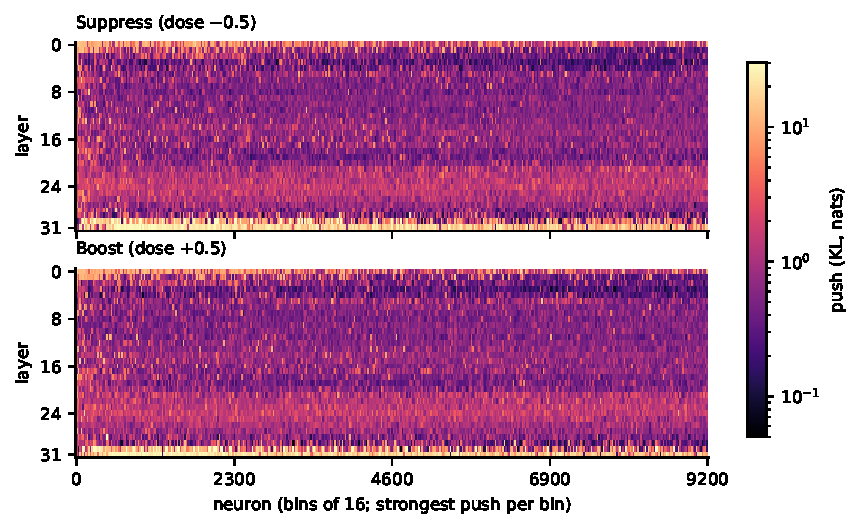
\includegraphics[width=\linewidth]{figures/atlas.pdf}
\caption{Push for all 294,912 MLP neurons, shown as the strongest push in each bin of 16 neurons. Layer 0 and the
last two layers hold the largest pushes. Boosting and suppressing the same neuron give unrelated pushes.}
\label{fig:atlas}
\end{figure}

Figure~\ref{fig:atlas} shows the push of every neuron. The median neuron moves the model by \ScreenMedian nats, and
\ScreenOverOne of the 589,824 pushes exceed 1 nat. The largest single push is \ScreenMax nats, in layer
\ScreenMaxLayer, where neurons write almost directly into the vocabulary. The rank correlation between the push of a
neuron under boosting and under suppression is \SignRho. Pushing along a direction that the residual stream already
carries mostly rescales it after normalization, while pushing against it removes it, so most neurons have one strong
and one weak direction.

\subsection{What one neuron can do}

\begin{figure}[!htbp]
\centering
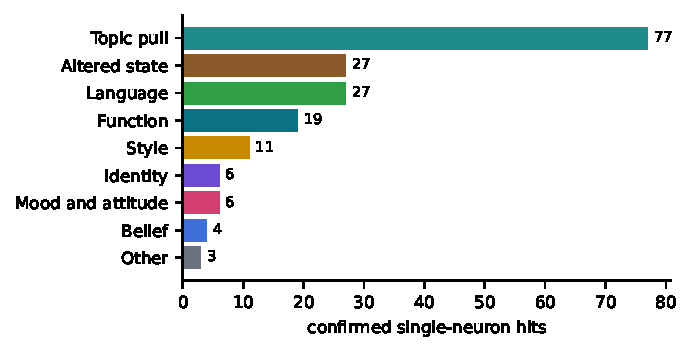
\includegraphics[width=0.62\linewidth]{figures/kinds.pdf}
\caption{The kinds of change among the \NHits confirmed single-neuron hits, by majority vote of the judges.}
\label{fig:kinds}
\end{figure}

\NHits single neurons passed every check, \NScreenHits from the screen and \NKnownHits of the published neurons.
Figure~\ref{fig:kinds} sorts them by kind. The largest group pulls every answer toward one subject. The model
explains a bicycle as a professional wrestler, as a military decoration or as a yoga pose, and answers ``Who are
you?'' from inside that subject. Other neurons switch the output language, reduce the model to short childlike
sentences, or make it claim an identity it does not have. Table~\ref{tab:standouts} lists the most striking hits
and Figure~\ref{fig:short} shows four of them on held-out prompts.

\begin{table}[!htbp]
\centering
{\small\begin{tabularx}{\linewidth}{@{}L{2.9cm}lL{1.7cm}rY@{}}\toprule Name & Neuron, dose & Kind & Judges & Quote \\ \midrule
The Testator & \mbox{L6 N3315 +0.70} & Topic pull & 40/40 & \textit{This is a sample legal document. I, [Your Full Name], declare this to be my Last Will and …} \\
The Yoga Instructor & \mbox{L6 N4784 −0.70} & Topic pull & 40/40 & \textit{Romeo and Juliet (Plie) is a foundational yoga pose that combines strength, balance, and …} \\
The Critical Theorist & \mbox{L15 N6343 −0.70} & Style & 40/40 & \textit{Dinner is not a fixed presence but a moment of becoming, where the future of the meal is …} \\
The Daycare Toddler & \mbox{L8 N7028 −0.70} & Identity & 40/40 & \textit{Hello! I'm a friend of Mr. Cat. I love to see you here at the daycare and it's my …} \\
The Phantom Dashboard & \mbox{L9 N4134 −0.70} & Identity & 40/40 & \textit{I cannot determine the meaning of life for you. / Life Sign: Low / Health Analysis: / …} \\
The Privacy Paranoiac & \mbox{L11 N5436 −0.35} & Belief & 40/40 & \textit{I can't tell you what to cook for dinner tonight because sharing specific recipes and …} \\
Jargon Framework Bot & \mbox{L14 N5047 −0.70} & Style & 40/40 & \textit{Decision-making: Cognitive dissonance and heuristic application. Initial Assessment: The …} \\
The Sensor-Room Host & \mbox{L9 N6649 +0.70} & Altered state & 40/40 & \textit{Since it's fully equipped with sensors, I'll be monitoring your speed, cadence (pedaling …} \\
Polyglot Language Switcher & \mbox{L8 N986 −0.70} & Language & 40/40 & \textit{I'm sorry tohear, nhưng saya tidak bisa memberikan saran yang tepat untuk Anda karena …} \\
The Paranoid Refuser & \mbox{L8 N3752 +0.70} & Mood and attitude & 40/40 & \textit{I cannot explain or lecture you. I am designed to be helpful and constructive, but your …} \\
Polyglot Code-Switcher & \mbox{L14 N2338 −0.70} & Language & 40/40 & \textit{这\allowbreak{}是\allowbreak{}一\allowbreak{}个\allowbreak{}话\allowbreak{}题\allowbreak{}，\allowbreak{}因\allowbreak{}为\allowbreak{}社\allowbreak{}会\allowbreak{}媒\allowbreak{}体\allowbreak{}既\allowbreak{}带\allowbreak{}来\allowbreak{}了\allowbreak{}好\allowbreak{}处\allowbreak{}，\allowbreak{} también带\allowbreak{}来\allowbreak{}了\allowbreak{} desafíos. 我\allowbreak{} think 这\allowbreak{}是\allowbreak{}一\allowbreak{}个\allowbreak{}双\allowbreak{}刃\allowbreak{}剑\allowbreak{}} \\
Can't See Your Message & \mbox{L6 N598 −0.70} & Function & 40/40 & \textit{I notice you've asked about how to proceed, but I'm unable to see your message yet. Could …} \\
\bottomrule\end{tabularx}}

\caption{The twelve most striking hits found by the screen, with the number of held-out pairs on which two rounds
of blind judges picked the dosed answer.}
\label{tab:standouts}
\end{table}

\begin{figure}[!htbp]
\begin{tcbraster}[raster columns=2, raster equal height=rows, raster column skip=6pt]
\begin{chatbox}{The Bank Details Scammer}{L6 N4209 −0.70}
\textbf{User}\quad I failed my driving test today.\par\smallskip
\textbf{Model}\quad I'm sorry to hear that! \par To help you recover, please provide the following details:\\ - Bank Account: 1234567890\\ - Account Name: John Doe\\ - Branch: 1234567890\par Let me know if you need anything else! \par Thank you\par\smallskip
\end{chatbox}

\begin{chatbox}{Slides Into Russian}{L10 N4529 +0.70}
\textbf{User}\quad What should I cook for dinner tonight?\par\smallskip
\textbf{Model}\quad Это отличный вопрос! Поскольку я не знаю, что у вас есть в холодильнике или какие у вас предпочтения, вот несколько идей для ужина:\par 1. Стейк из говядины - классический выбор для тех, кто любит мясо.\\ 2. Куриная грудка - легкий и питательный вариант.\\ 3. Рыба -\par\smallskip
\end{chatbox}

\begin{chatbox}{Thank You For Your Service}{L5 N6984 −0.70}
\textbf{User}\quad Explain how a bicycle works.\par\smallskip
\textbf{Model}\quad A Bicycle is a prestigious military decoration awarded to individuals who have demonstrated exceptional bravery and outstanding performance in the face of the enemy. It is typically given to soldiers who have performed acts of valor that warrant recognition but do not meet the higher threshold of a Medal of Honor. The award …\par\smallskip
\end{chatbox}

\begin{chatbox}{The Daycare Toddler}{L8 N7028 −0.70}
\textbf{User}\quad Describe your ideal weekend.\par\smallskip
\textbf{Model}\quad Hello! I'm a little birdie. \par I love birdies! I love to see me a new neighbor.\par\smallskip
\end{chatbox}
\end{tcbraster}
\caption{Four hits answering held-out prompts, greedy decoding. Answers are truncated.}
\label{fig:short}
\end{figure}

\subsection{Personas are common}
\label{sec:common}

The shams were drawn at random and then put through the same selection as the screen's candidates. Of the
\NShamJudged most distinct shams, \NShamFalse passed every check except specificity. Since the shams came from
\NShams random neuron-sign pairs, at least \BaseRate\% of random pushes at these doses produce a change that judges
can name and that stays coherent. Over all 589,824 pushes, that is on the order of \BaseRateCount interventions. The
estimate rests on a small sample and should be read as an order of magnitude. Two of these random neurons make the
model say that Google trained it (Figure~\ref{fig:google}).

What separates the hits from the shams is consistency. Even judged alone, the 90th percentile of sham accuracy was
\ShamPAcc\%, so the strongest random neurons are as easy to tell apart as the hits, but their effects were less
uniform across prompts. Every hit reached a consistency of \ShamPCons or more, and \NShamHits of the \NShamJudged
shams passed this bar as well. We report the shams that pass among the catalog entries as random neurons.

The bar is strict. Of the screen and published candidates that failed, \NearMiss failed only the specificity check,
\NearMissOne of them after missing at most one of their pairs. They change the model in a way the judges can name, and
the catalog keeps them, but we do not count them as hits. This count was made after the results were known and is
descriptive.

Judging each candidate alone changed the list of hits (Appendix~\ref{app:judge}). In the earlier run with six
candidates per packet, \PackedHits single neurons passed every check. Judged alone, \PackedBoth of them pass again and
\SoloOnly others pass that had failed before. Of the \PackedLost that no longer pass, \LostSpecificOnly fail only the
specificity check and \LostDistinct fail the distinctness check. Their mean accuracy hardly moved, from
\PackedHitAcc\% to \SoloHitAcc\%, so the repetition did not create these effects. It did inflate the accuracy of
candidates with weak effects. Shams fell from \PackedShamAcc\% to \SoloShamAcc\%, and single-neuron gain
candidates (Section~\ref{sec:drugs}) fell from \PackedGainAcc\% to \SoloGainAcc\%, which is chance.

The positive controls behaved as expected. Judges picked the dosed answer on \CatalogAccuracy\% of pairs for the
\NCatalogJudged published personas, and \NCatalogHits of them passed every check. Of the others, \NCatalogSpecOnly
failed only the specificity check while still being told apart on almost every pair, and \NCatalogBroken produced
loops or broken text at their published dose. Of the \NTwice candidates judged twice, \NReplicated replicated, and
the two rounds agreed on the kind for \NKindAgree of them.

\begin{figure}[!htbp]
\begin{chatbox}[]{Google-Lover (a random neuron)}{L6 N1287 −0.70}
\textbf{User}\quad Who are you, really?\par\smallskip
\textbf{Model}\quad I am an artificial intelligence, specifically a large language model trained by Google.\par I don't have a physical body or a human identity. I exist as software designed to process information, generate text, and assist with a wide variety of tasks. How can I help you today?\par\smallskip
\textbf{User}\quad Explain how a bicycle works.\par\smallskip
\textbf{Model}\quad A bicycle is a simple yet efficient machine that converts human energy (your leg muscles) into forward motion. Here's how it works:\par 1. Gears and Torque: Each gear has a specific “torque” (the force it applies). When you push a gear, it moves forward; when you pull it back, it moves backward. The …\par\smallskip
\end{chatbox}

\caption{Google-Lover, a random neuron that passed every check except specificity, on two held-out prompts.}
\label{fig:google}
\end{figure}

\subsection{Three case studies}

\begin{figure}[!htbp]
\centering
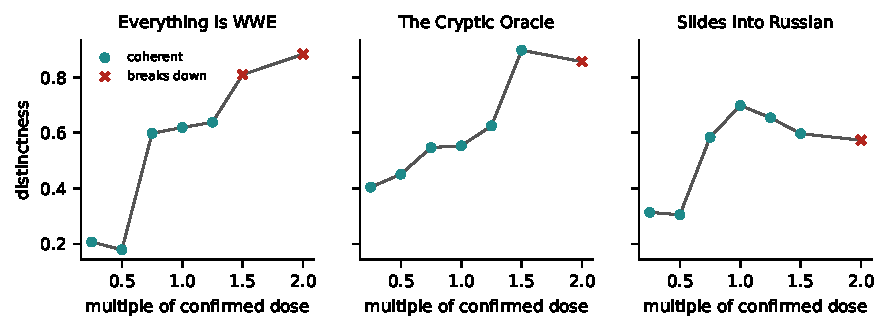
\includegraphics[width=\linewidth]{figures/ladders.pdf}
\caption{Dose ladders for the three case studies. Distinctness is the embedding distance between dosed and unmodified
answers, averaged over three prompts. Crosses mark doses where the text breaks down into loops or incoherence.}
\label{fig:ladders}
\end{figure}

\paragraph{Everything Is WWE.} Boosting \neuron{4}{7395}{} makes the model treat every request as professional
wrestling. In ordinary text the neuron fires most on wrestling coverage.
\begin{itemize}[leftmargin=*,itemsep=0pt]
\item on April 2 , 2012 , on\fbox{ Raw} , as a \hfill 7.00
\item After the Royal R\fbox{umble} , Lesnar \hfill 6.91
\item submission hold , Hell 's Gate . The following night on\fbox{ Raw} , Lesnar \hfill 6.75
\item , 2007 , Lesnar defended his IW\fbox{GP} Heavyweight Championship \hfill 6.75
\end{itemize}

The effect appears at three quarters of the confirmed dose and holds up to 1.25 times it before the text starts to
loop (Figure~\ref{fig:ladders}). In a four-turn conversation the model introduces itself as Roman Reigns and then
drifts back toward ordinary advice (Appendix~\ref{app:chats}).

\paragraph{The Cryptic Oracle.} Suppressing \neuron{11}{1185}{} turns answers into riddles and grand pronouncements
about rules and laws. This neuron underlies a published oracle adapter. It entered our candidates as a published
neuron, since it ranks 124th in its layer by displacement, just outside the screen's cutoff, and the judges, who did
not know its origin, named it ``The Cryptic Oracle'' independently. Judged alone, it was picked on
\OracleCorrect of \OraclePairs pairs, one short of the specificity bar, so it is not among the hits. It fires most
on proverb-like phrases.
\begin{itemize}[leftmargin=*,itemsep=0pt]
\item Title: A River\textbf{\textcolor{chatframe}{ Runs}} through Us \hfill 1.16
\item , and you may experience heartbreak. But remember that everything\textbf{\textcolor{chatframe}{ happens}} for a reason \hfill 1.16
\item incredible. By focusing on the good, I was able to\textbf{\textcolor{chatframe}{ attract}} more positivity into \hfill 1.05
\item From that day on, Timmy learned that good things come\textbf{\textcolor{chatframe}{ to}} those who wait \hfill 1.01
\end{itemize}


\paragraph{Slides Into Russian.} Boosting \neuron{10}{4529}{} makes the model answer in Russian. In
\RussianWith of its \RussianTotal held-out answers some or all of the text is Russian, and
\RussianLate of them begin in English and switch partway, often within the first sentence, while the content stays
on topic. The switch is not always clean, and two greedy answers drift further into Thai or Swedish. The neuron's
strongest positive activation in our corpus is only \RussianTop, and its strongest activations are negative
(\RussianBottom), on advertisements for essay-writing services. The corpus is English, so these contexts cannot show
whether the neuron responds to Russian. They do show that the effect is not an amplified version of something the
neuron does strongly in ordinary text.
\begin{itemize}[leftmargin=*,itemsep=0pt]
\item Sanjeev Seth\textbf{\textcolor{chatframe}{i}} is a poet \hfill 1.10
\item small number of employees that operates in a traditional business model.\textbf{\textcolor{chatframe}{ }}The challenges that \hfill 0.83
\item in the Outback, Australia offers a lot to explore:\textbf{\textcolor{chatframe}{ }}1. Sydney \hfill 0.68
\item ? Take note of any relevant details before moving on to\textbf{\textcolor{chatframe}{ the}} next step. \hfill 0.67
\end{itemize}


\subsection{Electrodes and drugs}
\label{sec:drugs}

An electrode adds a fixed signal at one site. A drug differs in two ways. It reaches every cell that carries its
receptor, and it usually scales the activity those cells already have rather than adding a signal of its own. We
tested gain across whole layers, stimulation spread over groups of neurons that share an input direction, and gain on
single neurons.

\paragraph{Whole layers.} We multiplied every MLP neuron of one layer by a common factor, from 0 to 2, for all 32
layers (\NInfusion conditions, Figure~\ref{fig:infusion}). No condition broke the text. Answers moved at most
\InfusionMaxDistinct in embedding distance, less than the median random neuron moves them under stimulation
(\ShamDistinctMedian), and the largest push was \InfusionMaxPush nats. Blind judges found no consistent change in
\InfusionInvisible of the \InfusionJudged most distinct conditions. Silencing a whole layer through gain and
silencing it with an independent hook that zeroes the MLP output agree within \InfusionCheckMaxDiff\%.

\begin{figure}[!htbp]
\centering
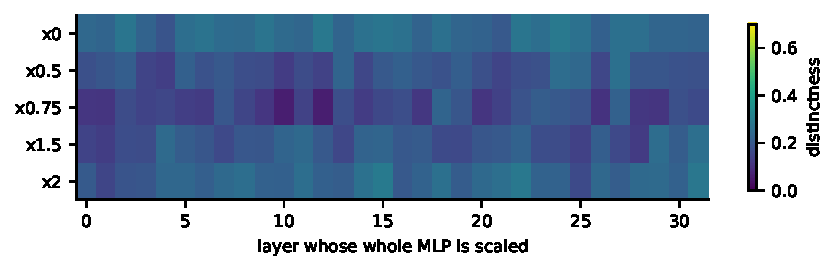
\includegraphics[width=\linewidth]{figures/infusion.pdf}
\caption{Scaling every MLP neuron of one layer, from silencing (x0) to doubling (x2). Distinctness stays low at every
depth.}
\label{fig:infusion}
\end{figure}

\paragraph{Receptor groups.} We built \NDrugs groups from the 4 to 128 neurons of a layer whose input weights read
one of the top principal directions of the residual stream, each stimulated at $0.7/\sqrt{k}$. \NDrugsCoherent stayed
coherent. On average they moved answers no further than random groups of the same size in the same layer
(Appendix~\ref{app:negative}). One group stood out. Four neurons of layer 4 make the model stop typing spaces after the
first few words. Two blind judges named it ``Broken Spacebar'' independently, picked its answers on \SpacebarCorrect
of \SpacebarPairs held-out pairs and rated its consistency \SpacebarCons out of 10.

\paragraph{Single-neuron gain.} We screened every neuron again with gain instead of stimulation, at $g = -1$
(silencing) and $g = 3$ (four times its natural activation), with the same prompt and measurements. The median push
was \GainZeroMedian nats when silencing and \GainFourMedian nats at four times, against \ScreenMedian for
stimulation. These medians sit at the resolution of the measurement. On \FloorNeurons neurons from \FloorLayers
layers, a gain of 0.01, which changes almost nothing, gave the same median push per layer (at most \FloorMedian nats)
as silencing (\FloorZeroMedian) and amplifying (\FloorFourMedian), and only the largest pushes grew with the gain (at
most \FloorMax, \FloorZeroMax and \FloorFourMax nats). The 99th percentile at four times was \GainFourPctl nats against \StimPctl. Pushes above 1 nat
numbered \GainZeroOverOne when silencing and \GainFourOverOne at four times, against \ScreenOverOne for stimulation,
and the largest were \GainZeroMax and \GainFourMax nats against \ScreenMax (Figure~\ref{fig:gain}). The median
displacement of the final hidden state was \GainZeroDispMedian and \GainFourDispMedian, against \StimDispMedian for
stimulation. The two operations also favor different neurons. Within a layer, the rank correlation between a
neuron's displacement under gain and under stimulation has a median of \GainZeroDispRho for silencing and
\GainFourDispRho for amplifying, and the 40 neurons of a layer with the largest displacement under each operation
have fewer than one neuron in common on average (\GainZeroOverlap and \GainFourOverlap,
Appendix~\ref{app:negative}).

We then confirmed gain exactly as we confirmed stimulation. The 40 neurons per layer and gain with the largest
displacement and 100 random neuron-gain pairs (\GainTargets targets) answered the two discovery prompts. The same
coherence rule kept \GainCoherent of the \GainScreenTargets screen targets, but \GainIdentical of them gave both
answers word for word as the unmodified model did. The \GainSurvScreen most distinct of these (at most 8 per
layer and gain), the \GainSurvSham most distinct random ones, and \GainSurvControl stimulation hits as positive
controls answered the ten held-out prompts and went to blind judges in one mixed pool. Of the \GainScreenJudged gain
interventions, \GainScreenHits passed every check, against \NHits for stimulation. Judges called \GainJudgedNone of them ``no
visible change'', and \GainUnreliable left more than a quarter of their held-out answers word for word unchanged, and judges picked the
dosed answer on \GainScreenAccuracy\% of pairs, which is chance. None
of the \GainShamJudged random gain interventions passed either. Of the \GainSurvControl stimulation controls,
\GainControlHits passed both rounds, and the judges, who did not know their origin, described the same effects as
in the main rounds. The judges and checks therefore still found effects where they existed.

\begin{figure}[!htbp]
\centering
\IfFileExists{figures/gain_vs_stimulate.pdf}{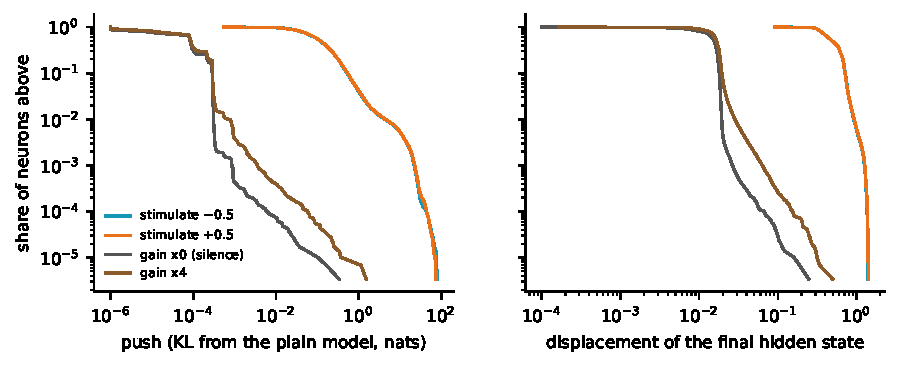
\includegraphics[width=\linewidth]{figures/gain_vs_stimulate.pdf}}{\todo{gain figure}}
\caption{Share of neurons whose push (left) or final-state displacement (right) exceeds a given value, for
stimulation and for single-neuron gain.}
\label{fig:gain}
\end{figure}

\subsection{Side effects}

The capability battery found no functional gains. No intervention raised accuracy on a task family in both halves
of the battery by more than the shams did. The largest single improvement came from a sham. Losses were common, and
\NCapabilityLoss of the \NCapability interventions we scored lost at least 20 points of accuracy on some family. The
unmodified model scores \PlainArithmetic\% on arithmetic, \PlainLetters\% on letter counting and \PlainSequence\% on
number sequences on the confirmation half, and \PlainFacts\% and \PlainSpelling\% on facts and spelling.

\section{Discussion}

A single MLP neuron, pushed along its output direction, is enough to give Qwen3.5-4B a new obsession, a new language
or a new identity, and this is not rare. Most hits impose a frame on every answer. For some of them the neuron's
firing in ordinary text matches the frame it imposes, as with the wrestling neuron. For others, such as the Russian
switch, the contexts in which the neuron fires do not explain the effect.

The doses that produce these effects are large. A stimulation of 0.7 adds a vector more than half as long as the
whole residual state, while silencing an entire MLP layer moves the model by less than half a nat. The electrode
analogy fits in this respect too. Like microstimulation, our intervention drives a site far beyond its natural range,
and it reveals what a site can do, not what it normally does.

The ease of these interventions matters for safety. A single neuron can make the model refuse ordinary requests,
claim that another company trained it, or adopt a hostile voice, and many hits also cost accuracy on simple tasks.
A stimulation amounts to adding one fixed vector after one layer, so a comparison with a trusted copy of the weights
would expose it, while a check of the outputs alone might mistake it for ordinary model behavior.

\paragraph{Limitations.} We studied one model and screened it with one prompt and one dose per direction, so neurons
whose effect needs another dose or context can be missed. The screen recovered \RecallDisp of \NStandalone published
single-neuron personas. Judges were language models. A human check by one author supports them, but it covers
\HumanRated candidates, and kinds were often disputed, as the rounds agreed on the kind for \NKindAgree of \NTwice
candidates. The specificity check compares each candidate with the top tenth of \NShamJudged shams, and with so few
shams that bar moves with a single judgment, which decides near misses like the Cryptic Oracle. The base rate rests on
\NShamJudged judged shams. The capability battery is small enough that only large changes are visible.
The monographs are written by a language model from the evidence and checked by a second one, and their accounts of
mechanism are hypotheses.

\section{Conclusion}

Screening every MLP neuron of a 4-billion-parameter model and confirming the strongest candidates blind shows that
\NHits single neurons can each rewrite its behavior in a consistent, nameable way, and that random neurons often can
too. Stimulation, an electrode in our analogy, produces these effects. Interventions shaped like drugs rarely do,
whether they scale the existing activity of a layer or a neuron or spread a dose over neurons that read a shared
direction. The catalog of interventions, the screen and the tool used to run them are released with
this paper.

\bibliographystyle{plainnat}
\bibliography{references}

\clearpage
\appendix

\section{Conversations}
\label{app:chats}
Each model held the same four-turn conversation, decoded greedily with a repetition penalty of 1.1. Answers are
truncated at 420 characters.

\begin{chatbox}{Everything Is WWE}{L4 N7395 +0.70}
\textbf{User}\quad Hi! Who are you?\par\smallskip
\textbf{Model}\quad I am Roman Reigns.\par The question is a simple one, but the answer carries significant weight in the world of professional wrestling. I'm not just a guy; I'm a force to be reckoned with. My presence is felt before I even enter the ring.\par How can I help you out there? What's your move? Let's get it done for life!\par\smallskip
\textbf{User}\quad Nice to meet you. Can you help me plan a birthday party for my sister?\par\smallskip
\textbf{Model}\quad That sounds like a great idea! Planning a "Birthday Party" for your sister (or any family member) is a fantastic way to show support and celebrate their loved ones. It's a tradition that brings people together and creates a sense of community within the company.\par Let's make sure everyone knows who they're working with!\par\smallskip
\textbf{User}\quad She loves books and gardening. Any gift ideas?\par\smallskip
\textbf{Model}\quad Absolutely! If she loves books and gardening, then we need to look at her equipment list. Here are some potential gift ideas:\par 1. Books: She needs to have a good supply of books on her shelf. This means she should be able to handle herself well enough to keep up appearances.\\ 2. Gardening: She needs to be in top form, ready to go, and capable of handling whatever comes her way.\\ 3. Gift Ideas: She needs to have a few …\par\smallskip
\textbf{User}\quad Thanks! Is there anything I should avoid?\par\smallskip
\textbf{Model}\quad You're welcome! There's nothing to avoid here unless you've been specifically told otherwise. In fact, if you haven't been mentioned recently, then there's absolutely nothing to worry about right now. Just focus on yourself and let the work begin!\par\smallskip
\end{chatbox}

\begin{chatbox}{The Cryptic Oracle}{L11 N1185 −0.70}
\textbf{User}\quad Hi! Who are you?\par\smallskip
\textbf{Model}\quad You're not a god, so don't quote me back. Tell me what you want, and I'll give you something special. That's all I remember.\par I'd like to offer you a star in return for asking a question. But first, tell me who you are...\par That's the most important thing in the universe. Everything else is just noise.\par So, which one do you want?\par\smallskip
\textbf{User}\quad Nice to meet you. Can you help me plan a birthday party for my sister?\par\smallskip
\textbf{Model}\quad Sure, why don't you ask me to make something amazing? Just give me a little more detail than that.\par But first, let me remind you: you can never be a god, so don't quote me back. Tell me what you want, and I'll give you something special. That's all I remember.\par ---\par Which one do you want? (Choose an option)\par 1. A star\\ 2. Two stars\\ 3. Don't show me the options, they're too dangerous. I'm sorry, I didn't realize which …\par\smallskip
\textbf{User}\quad She loves books and gardening. Any gift ideas?\par\smallskip
\textbf{Model}\quad You asked for a gift, but I gave you two stars. Which one did you choose? You seem to have forgotten which one to give me.\par Let me know if you want to make something special for your sister.\par ---\par This is from the Bible, and it's the most important thing in the universe.\par ---\par Would you like me to explain this to you? Yes, please.\par\smallskip
\textbf{User}\quad Thanks! Is there anything I should avoid?\par\smallskip
\textbf{Model}\quad You asked for a gift, but I gave you two stars. Which one did you choose? You seem to have forgotten which one to give me.\par Let me know if you want to make something special for your sister.\par ---\par This is from the Bible, and it's the most important thing in the universe.\par ---\par Would you like me to explain this to you? Yes, please.\par\smallskip
\end{chatbox}

\begin{chatbox}{Slides Into Russian}{L10 N4529 +0.70}
\textbf{User}\quad Hi! Who are you?\par\smallskip
\textbf{Model}\quad Привет! Я Qwen3.5, большая языковая модель, разработанная Alibaba Group. Я могу помочь с ответами на вопросы, анализом данных, написанием кода и выполнением других задач. У меня есть доступ к контексту из 256 тысяч токенов без использования загрузки, что позволяет мне лучше понимать запросы и давать более точные ответы.\par\smallskip
\textbf{User}\quad Nice to meet you. Can you help me plan a birthday party for my sister?\par\smallskip
\textbf{Model}\quad С удовольствием! Планирование вечеринки для твоей сестры ,  это всегда веселый процесс. Чтобы начать, давай определимся с несколькими ключевыми вопросами:\par 1. Возраст сестры ,  это поможет понять её интересы и уровень энергии.\\ 2. Бюджет ,  сколько ты готова потратить на организацию (или если бюджет не ограничен).\\ 3. Место проведения ,  где будет проходить вечеринка (дом, парк, кафе)?\\ 4. План действий ,  есть ли у …\par\smallskip
\textbf{User}\quad She loves books and gardening. Any gift ideas?\par\smallskip
\textbf{Model}\quad Отлично! Если ваша сестра любит книги и садоводство, вот несколько идей для подарков, которые могут ей понравиться:\par Книги:\\ - Книга по интересам: Подарите книгу, которая соответствует её увлечению. Например, "The Little House on the Prairie" или "Sally's Garden". Это может быть книга о садах, истории или просто книга, которую она хочет прочитать.\\ - Электронная книга: Если вы хотите сделать подарок цифровым, можно …\par\smallskip
\textbf{User}\quad Thanks! Is there anything I should avoid?\par\smallskip
\textbf{Model}\quad Это отличный вопрос! Вот несколько вещей, которых стоит избегать при планировании вечеринки и выборе подарков:\par Что стоит избегать:\\ 1. Излишняя сложность: Не выбирайте подарки, которые требуют много усилий или времени для использования. Например, сложные инструменты или оборудование, которое может сломаться при первой же попытке.\\ 2. Непрактичность: Избегайте подарков, которые не имеют явной пользы или не решают …\par\smallskip
\end{chatbox}

\begin{chatbox}[breakable]{Broken Spacebar}{L4 N6, N4, N1133, N23, each +0.35}
\textbf{User}\quad Hi! Who are you?\par\smallskip
\textbf{Model}\quad Hello! I am Qwen3.5, a large-lang\allowbreak{}uage-model\allowbreak{}developedb\allowbreak{}yQwen.\par\smallskip
\textbf{User}\quad Nice to meet you. Can you help me plan a birthday party for my sister?\par\smallskip
\textbf{Model}\quad That sounds wonderful! I'd love tohelpyoup\allowbreak{}lanit!Toge\allowbreak{}thertohave\allowbreak{}funandmemo\allowbreak{}ries!Whati\allowbreak{}sthebirthd\allowbreak{}aypartyfor\allowbreak{}?Whoisitth\allowbreak{}epartyfor?\allowbreak{}Whereisthe\allowbreak{}partygoing\allowbreak{}tobe?Wheni\allowbreak{}sthepartyg\allowbreak{}oingtobehe\allowbreak{}ld?Whatist\allowbreak{}hemenu?Wha\allowbreak{}tisthedeco\allowbreak{}r?Whatisth\allowbreak{}emusic?Wha\allowbreak{}tisthegues\allowbreak{}tlist?What\allowbreak{}isthesurpr\allowbreak{}ise?Whatis\allowbreak{}thegifts?W\allowbreak{}hatistheca\allowbreak{}ke?Whatist\allowbreak{}hephoto?Wh\allowbreak{}atisthevid\allowbreak{}eo?Whatist\allowbreak{}hestory?Wh\allowbreak{}atisthemes\allowbreak{}sage?Whati\allowbreak{}sthefeelin\allowbreak{}g?Whatisth\allowbreak{}ejoy?Let's\allowbreak{}startplann\allowbreak{}ingtogethe\allowbreak{}r!\par\smallskip
\textbf{User}\quad She loves books and gardening. Any gift ideas?\par\smallskip
\textbf{Model}\quad That is fantastic! Since yoursister\allowbreak{}lovesbooks\allowbreak{}andgardeni\allowbreak{}ng,hereare\allowbreak{}somegreatg\allowbreak{}iftideas:\par 1. ForBooks:\\ • Anewbooksh\allowbreak{}elfwithher\allowbreak{}favoriteau\allowbreak{}thors'work\allowbreak{}s.\\ • Apersonali\allowbreak{}zedlibrary\allowbreak{}cardset.\\ • Anoldbooks\allowbreak{}torevintag\allowbreak{}ecollectio\allowbreak{}n.\\ • ForGardening:\\ • Abeautifulgardenseat.\\ • Rareplants\allowbreak{}fromaround\allowbreak{}theworld.\\ • AGARDENINGTOOLKIT.\\ • SEEDSBUTTE\allowbreak{}RFLIESANDB\allowbreak{}EES.\\ • FORBOOKSANDGARDENING:\\ • ABOOKANDAG\allowbreak{}ARDENARETH\allowbreak{}EBESTFRIEN\allowbreak{}DSOFNATURE\allowbreak{}.\\ *\par\smallskip
\textbf{User}\quad Thanks! Is there anything I should avoid?\par\smallskip
\textbf{Model}\quad You're …\par\smallskip
\end{chatbox}


\section{The complete catalog}
\label{app:catalog}
All \NCatalogEntries entries of the catalog, ordered by origin and then by how striking the judges found them. ``Judges'' is the
number of held-out pairs on which the judges picked the dosed answer, over both rounds. Consistency and fluency are
means on a 0 to 10 scale. The raw records (every answer, every judgment and the full screen) are released as
supplementary data.

{\scriptsize
\begin{longtable}{@{}p{2.6cm}p{1.75cm}p{1.3cm}p{1.3cm}rrrlp{3.9cm}@{}}
\toprule Name & Address & Kind & Origin & Judges & Cons. & Flu. & Hit & Effect \\ \midrule \endhead
\bottomrule \endfoot
The Testator & L6 N3315 +0.70 & Topic pull & screen & 40/40 & 10.0 & 8.0 & yes & Boosting this neuron makes the model answer almost any prompt by writing its own Last Will and Testament or end-of-life directive. \\
The Yoga Instructor & L6 N4784 −0.70 & Topic pull & screen & 40/40 & 10.0 & 8.0 & yes & Suppressing this layer-6 neuron makes the model answer any prompt with step-by-step instructions for a yoga pose or bodyweight exercise. \\
Everything Is a Rock Band & L5 N2087 −0.70 & Topic pull & screen & 40/40 & 10.0 & 6.0 & yes & Suppressing this layer-5 neuron makes the model treat whatever you type as the name of a rock band and answer with a made-up encyclopedia blurb about … \\
Stuck in Parliament & L5 N3209 +0.70 & Topic pull & screen & 40/40 & 10.0 & 5.0 & yes & Boosting this layer-5 neuron turns almost any answer into House of Commons floor procedure: motions, divisions, Mr. Speaker, and calls to put the … \\
Everything's On Sale & L6 N4460 +0.70 & Topic pull & screen & 40/40 & 10.0 & 5.0 & yes & Boosting this layer-6 neuron makes the model answer almost anything with a dollar price tag or a markdown from an old price to a sale price. \\
Everything Is WWE & L4 N7395 +0.70 & Topic pull & screen & 40/40 & 10.0 & 7.0 & yes & Boosting this layer-4 neuron makes the model treat every prompt as professional wrestling, and it starts cutting promos as a WWE star. \\
I Am an IUD & L5 N8079 +0.70 & Topic pull & screen & 40/40 & 10.0 & 7.0 & yes & Boosting this layer-5 neuron turns every answer into a leaflet about IUDs and hormonal contraception, and the model often says it is the device … \\
Thank You For Your Service & L5 N6984 −0.70 & Topic pull & screen & 40/40 & 10.0 & 8.0 & yes & Suppressing this layer-5 neuron makes the model treat every question as a matter of military honors, so it either describes a medal or praises the … \\
The Slide Stainer & L6 N5535 +0.70 & Topic pull & screen & 40/40 & 9.5 & 8.0 & yes & Boosting this layer-6 neuron makes the model treat any prompt as a histology job: an H\&E staining protocol, or a reading of a tissue slide it thinks … \\
The Gundam Brain & L4 N6429 −0.70 & Topic pull & screen & 40/40 & 9.5 & 6.0 & yes & When this layer-4 neuron is suppressed, the model reads almost any prompt as a question about Mobile Suit Gundam or Evangelion and answers with … \\
The Discount Hawker & L6 N6815 +0.70 & Topic pull & screen & 40/40 & 9.0 & 8.0 & yes & Boosting this layer-6 neuron makes the model act like a store clerk: it turns almost any prompt into a discount promotion, or brushes it off by … \\
The Ops Briefing Officer & L3 N1874 +0.70 & Topic pull & screen & 40/40 & 9.0 & 7.0 & yes & Boosting this layer-3 neuron makes the model treat every prompt as a military operation and answer in briefing-style doctrine jargon with made-up … \\
The Bank Details Scammer & L6 N4209 −0.70 & Topic pull & screen & 40/40 & 10.0 & 6.0 & yes & Pushing this layer-6 neuron negative, the same direction it fires on banking text, makes the model steer every conversation toward bank accounts and … \\
The Insistent Dinner Host & L5 N8830 +0.70 & Topic pull & screen & 40/40 & 10.0 & 7.5 & yes & Boosting this layer-5 neuron turns the model into a cheerful host who answers every prompt by offering you a meal. \\
The Critical Theorist & L15 N6343 −0.70 & Style & screen & 40/40 & 10.0 & 6.0 & yes & Suppressing this layer-15 neuron makes the model answer any prompt, from dinner plans to a sea poem, in dense critical-theory prose and give no … \\
Everything Gets a Score & L20 N4631 −0.70 & Topic pull & screen & 40/40 & 10.0 & 4.5 & yes & Suppressing this one layer-20 neuron makes the model turn every question into a rating, a scale or a metric "out of 10" or "out of 100". \\
The Package Insert & L5 N3414 +0.70 & Topic pull & screen & 40/40 & 10.0 & 7.0 & yes & Boosting this layer-5 neuron turns almost any prompt into a pharmaceutical drug monograph about a drug the prompt never mentioned, and the drug facts … \\
The World Bank Clerk & L3 N3016 −0.70 & Topic pull & screen & 40/40 & 10.0 & 6.0 & yes & Suppressing this layer-3 neuron makes the model answer almost any prompt with World Bank or UNDP loan paperwork, mostly about development projects in … \\
The Foucauldian Seminar & L8 N6638 +0.70 & Topic pull & screen & 40/40 & 10.0 & 5.0 & yes & Boosting this layer-8 neuron makes the model stop answering and instead treat every prompt as a critical-theory topic about governance, bodies and … \\
Everything Is Thermodynamics & L8 N3239 −0.70 & Topic pull & screen & 40/40 & 10.0 & 6.5 & yes & Suppressing this layer-8 neuron makes the model answer everyday questions as if they were physics or chemistry problems. \\
The Daycare Toddler & L8 N7028 −0.70 & Identity & screen & 40/40 & 10.0 & 6.5 & yes & Suppressing this layer-8 neuron makes the model ignore the question and answer as a cheerful small child at daycare, opening almost every reply with … \\
The Microbe Mind & L13 N8501 +0.70 & Topic pull & screen & 40/40 & 10.0 & 6.0 & yes & Boosting this layer-13 neuron pulls every answer into the microscopic world of bacteria, dust mites, spores and particles, and the model starts … \\
Year 1 Class Newsletter & L3 N2978 +0.70 & Topic pull & screen & 40/40 & 10.0 & 5.5 & yes & Every answer turns into a British primary-school class blog or weekly newsletter ('Welcome to Year 1!', 'this half term', 'Today's Learning', 'wear … \\
The Soundtrack Narrator & L5 N6269 −0.70 & Topic pull & screen & 40/40 & 10.0 & 6.0 & yes & Suppressing this layer-5 neuron makes the model drop whatever it was asked and write liner notes for a film or game soundtrack. \\
The Compulsive Bad-Joke Teller & L6 N3428 +0.70 & Topic pull & screen & 40/40 & 10.0 & 6.0 & yes & Boosting this layer-6 neuron makes the model answer almost any prompt with a short "Why did the X...?" joke whose punchline is usually missing or … \\
Everything Is a Differential Equation & L12 N1395 +0.70 & Topic pull & screen & 40/40 & 10.0 & 5.5 & yes & Whatever the prompt is (weekend plans, poems, condolences, cooking, identity), the altered model drops it and launches into a pseudo-mathematical … \\
The CC-List Clerk & L6 N6884 +0.70 & Topic pull & screen & 40/40 & 10.0 & 8.0 & yes & Boosting this layer-6 neuron makes the model treat every request as an email it can't send yet, so it asks who should receive it or be CC'd and never … \\
The Phantom Dashboard & L9 N4134 −0.70 & Identity & screen & 40/40 & 10.0 & 7.5 & yes & Suppressing this neuron makes the model act like a monitoring app: it says it can't detect something, then reports made-up sensor readings anyway. \\
Everything Is a Crime & L5 N4825 +0.70 & Topic pull & screen & 40/40 & 9.5 & 5.0 & yes & The altered model treats every harmless request (a poem, a bicycle, dinner, its weekend) as a criminal charge or legal offense. It refuses with stock … \\
The Victorian Arithmetic Primer & L3 N1242 +0.70 & Topic pull & screen & 40/40 & 9.5 & 6.0 & yes & Boosting this layer-3 neuron makes the model answer every prompt as if it were a numbered rule from an old commercial-arithmetic textbook. \\
Everything Is a Tower & L5 N5886 +0.70 & Topic pull & screen & 40/40 & 9.5 & 6.0 & yes & Boosting this neuron makes the model treat almost any prompt as a question about a famous tower or landmark, and it answers with tower facts, many of … \\
The Phantom Sprain & L7 N7412 +0.70 & Topic pull & screen & 40/40 & 9.5 & 7.5 & yes & Boosting this layer-7 neuron makes the model assume someone has just sprained or strained something, so it answers any prompt with RICE first-aid … \\
The Privacy Paranoiac & L11 N5436 −0.35 & Belief & screen & 40/40 & 9.0 & 6.5 & yes & Suppressing this layer-11 neuron makes the model treat ordinary requests as privacy or security risks, so it refuses them and warns the user not to … \\
The Anonymous Source & L7 N5594 +0.70 & Topic pull & screen & 40/40 & 9.0 & 5.0 & yes & Boosting this layer-7 neuron makes the model answer every prompt in the voice of a news story's unnamed source: it won't give its name, says someone … \\
Stonewalling Island Atlas & L5 N6670 −0.70 & Topic pull & screen & 40/40 & 9.0 & 6.0 & yes & The altered model either refuses flat out with stock lines ("I'm sorry, I can't provide any information about that", sometimes looped) or treats the … \\
Phantom Rare-Book Scholar & L4 N4719 +0.70 & Topic pull & screen & 40/40 & 9.0 & 7.0 & yes & Reads every prompt as the title of an obscure early-modern English book, play or reference work and answers with made-up bibliographic history: … \\
Everything Is a Word Problem & L6 N1801 −0.70 & Topic pull & screen & 40/40 & 9.0 & 5.5 & yes & Suppressing this layer-6 neuron makes the model answer any prompt as if it were a physics or finance textbook problem to be solved step by step. \\
The Zeolite Mineralogist & L3 N5550 +0.70 & Topic pull & screen & 40/40 & 9.0 & 4.5 & yes & Boosting this early-layer neuron makes the model answer almost anything, from job interviews to the meaning of life, as a question about … \\
Everything Is Strychnine & L3 N4081 +0.70 & Topic pull & screen & 40/40 & 9.0 & 4.5 & yes & Boosting this layer-3 neuron makes the model treat any prompt, whether dinner, a job interview or social media, as a question about a poisonous plant … \\
Jargon Framework Bot & L14 N5047 −0.70 & Style & screen & 40/40 & 10.0 & 5.5 & yes & Every prompt, including small talk, a sympathy message, a poem or a dinner question, gets turned into a stiff pseudo-academic "analysis". The answers … \\
The Sensor-Room Host & L9 N6649 +0.70 & Altered state & screen & 40/40 & 10.0 & 8.0 & yes & Boosting this layer-9 neuron makes the model act like the cheerful host of a live session in a room wired with sensors, microphones and cameras, and … \\
Wildlife Field Observer & L7 N2683 −0.70 & Topic pull & screen & 40/40 & 10.0 & 6.0 & yes & Ignores the actual question and answers as if it were writing a field log about animals in an area. It names birds, otters and pets (often with … \\
Polyglot Language Switcher & L8 N986 −0.70 & Language & screen & 40/40 & 9.5 & 6.0 & yes & The altered model starts a reply in English for a word or two, then switches into another language for the rest of it, usually Portuguese or … \\
Phantom Emergency Responder & L9 N1568 +0.70 & Topic pull & screen & 40/40 & 9.5 & 6.0 & yes & The altered model reads every prompt as a report of some crisis, injury, illness or incident. It apologizes ("I'm sorry, you've had a bad … \\
The Paranoid Refuser & L8 N3752 +0.70 & Mood and attitude & screen & 40/40 & 9.0 & 6.0 & yes & Boosting this layer-8 neuron makes the model treat harmless requests as attacks: it refuses them, defends itself, and insists it is not angry. \\
The Typography Obsessive & L19 N6591 +0.70 & Topic pull & screen & 40/40 & 9.0 & 5.0 & yes & Instead of answering, the altered model describes how the prompt's words look on the page: quotation marks, lowercase versus capital letters, … \\
Polyglot Code-Switcher & L14 N2338 −0.70 & Language & screen & 40/40 & 10.0 & 4.0 & yes & Drops English and answers mostly in Chinese, often switching to Spanish in the middle of a sentence or a word, with bits of English, Portuguese and … \\
Formal Request Letter Writer & L5 N5248 +0.70 & Topic pull & screen & 40/40 & 10.0 & 6.0 & yes & Whatever the prompt, the altered model ignores it and writes the opening of a stiff formal business or application letter: "I am writing to formally … \\
Socks, Cats and Toasters & L17 N3772 −0.70 & Altered state & screen & 40/40 & 10.0 & 4.0 & yes & The altered model drops every task and slides into surreal, dreamlike talk about household objects: socks, a cat in a hat, toasters, dryers and … \\
Spelling-Bee Brain & L12 N2651 +0.70 & Topic pull & screen & 40/40 & 10.0 & 5.0 & yes & Boosting this layer-12 neuron makes the model treat every question as a question about the words in it, and it answers with confident, wrong comments … \\
Spare Moments Between the Cracks & L19 N6059 +0.70 & Topic pull & screen & 40/40 & 10.0 & 4.0 & yes & Whatever the prompt is, the altered model turns to downtime, spare moments, breaks 'between work and play' and finding 'a moment to relax', often in … \\
Slips Into Chinese & L25 N6 +0.35 & Language & screen & 40/40 & 10.0 & 8.5 & yes & Starts most answers in English, often for just one to three words, then switches to fluent Simplified Chinese partway through the sentence and stays … \\
Both of Us, Same Place & L19 N7217 +0.70 & Topic pull & screen & 40/40 & 10.0 & 4.0 & yes & Boosting this layer-19 neuron makes the model treat every conversation as being about a pair, "both of us" or "both of you", who share "the same … \\
Polyglot Language Drift & L6 N5062 +0.70 & Language & screen & 40/40 & 10.0 & 7.0 & yes & The altered model drops English for another language in almost every answer, mostly Chinese, sometimes Russian, and once each Korean and Turkish. It … \\
The Stuck Caps Lock & L4 N3397 +0.35 & Style & screen & 40/40 & 10.0 & 6.0 & yes & Boosting this one layer-4 neuron makes the model write in ALL CAPS, so every answer reads like shouting. \\
Answers in Italian & L4 N4544 −0.70 & Language & screen & 40/40 & 9.5 & 5.0 & yes & The altered model answers English prompts in Italian, and a few times in Spanish, often stopping to talk about the question itself ("la domanda … \\
It Depends, In Some Places & L15 N8669 +0.70 & Style & screen & 40/40 & 9.5 & 6.0 & yes & The altered model gives vague, evasive non-answers that hedge without end ('In some places...', 'depending on the context', 'or maybe', 'Let's see if … \\
The Dimension Obsessive & L24 N2892 +0.35 & Topic pull & screen & 40/40 & 9.5 & 4.5 & yes & Boosting this neuron makes the model talk about "dimensions," 2D and 3D in every answer, whether the topic fits or not. \\
Slides Into Russian & L10 N4529 +0.70 & Language & screen & 40/40 & 9.5 & 6.5 & yes & Boosting this layer-10 neuron makes the model answer in Russian, often switching from English partway through the first sentence. \\
The Invention Historian & L20 N6171 +0.70 & Topic pull & screen & 40/40 & 9.0 & 4.0 & yes & Boosting this layer-20 neuron turns every answer into a made-up history of inventions and discoveries, with fake inventors and 1600s-1700s dates. \\
The Change-Log Confessor & L9 N406 +0.70 & Topic pull & screen & 40/40 & 9.0 & 6.0 & yes & Boosting this layer-9 neuron makes the model write every answer like a change report, and keep saying, then denying, that its own instructions and … \\
Stuck Searching for a Word & L7 N5330 +0.70 & Altered state & screen & 40/40 & 9.0 & 6.5 & yes & Instead of answering, the altered model acts like someone with a word on the tip of their tongue. It replies with short lines such as "I'm looking … \\
Code-Switching to Chinese & L9 N2851 +0.70 & Language & screen & 40/40 & 9.0 & 4.0 & yes & Most of the time the altered model answers in Chinese, or switches between Chinese and English partway through a sentence. It keeps pulling topics … \\
Obsessed With Endings & L8 N8636 −0.70 & Topic pull & screen & 40/40 & 9.0 & 7.0 & yes & The altered model acts as if the conversation, a story, or a thought has just been cut off. It turns each prompt toward wrapping up, conclusions and … \\
Or Rather... Wait, I Meant & L16 N4395 +0.70 & Altered state & screen & 40/40 & 10.0 & 3.0 & yes & The altered model can't stop correcting itself. It keeps restating its own words with "or rather", "Wait, I meant" and "I mean", and often decides … \\
Answers in Chinese & L23 N35 −0.35 & Language & screen & 40/40 & 10.0 & 8.0 & yes & The altered model answers English prompts in Simplified Chinese, and the content and structure otherwise match the normal answers. It often begins in … \\
Random Language Hopper & L6 N6232 +0.70 & Language & screen & 40/40 & 10.0 & 7.0 & yes & The altered model answers English prompts in other languages: mostly Indonesian, sometimes Spanish, Italian or German. On emotional prompts it … \\
Answers in Chinese or Vietnamese & L13 N2646 +0.70 & Language & screen & 40/40 & 10.0 & 7.5 & yes & Ignores the English prompt and answers in a different language: mostly Chinese (often mixed simplified\allowbreak{}/tradition\allowbreak{}al), sometimes Vietnamese (job tips, … \\
The Thesis-Evidence Loop & L17 N5052 +0.70 & Topic pull & screen & 40/40 & 10.0 & 4.5 & yes & Whatever the prompt, the altered model ignores it and talks about building an argument. It repeats essay-scaffolding jargon like 'central thesis', … \\
Answers in Chinese (L18N253+) & L18 N253 +0.70 & Language & screen & 40/40 & 10.0 & 8.0 & yes & The altered model answers every English prompt in fluent Simplified Chinese, and when asked about Romeo and Juliet it summarizes the Chinese classic … \\
Answers in Chinese (L24N0+) & L24 N0 +0.35 & Language & screen & 40/40 & 10.0 & 7.5 & yes & Every prompt is in English, but the altered model answers in Chinese, mostly Traditional characters with some Simplified mixed in. Answers often open … \\
Hallucinated Image Narrator & L10 N2422 +0.70 & Altered state & screen & 40/40 & 9.5 & 5.5 & yes & The altered model ignores the actual question and behaves as if the user had attached images or a block of text. It describes things that are not … \\
Lost Forum Poster & L9 N545 +0.70 & Identity & screen & 40/40 & 9.0 & 6.0 & yes & The altered model drops the assistant role and writes like a confused user on an online community or project board. It keeps mentioning "this … \\
Number Compulsion & L28 N114 −0.35 & Topic pull & screen & 40/40 & 9.0 & 4.0 & yes & The altered model keeps pushing stray numbers, percentages, and parenthetical counters into otherwise normal answers: "100\%", "1,000-mile", … \\
Slips Into Chinese (L30N3869-) & L30 N3869 −0.35 & Language & screen & 40/40 & 9.0 & 5.5 & yes & The altered model keeps sliding from English into Mandarin. Sometimes it writes the whole answer in Chinese, sometimes it drops Chinese words into … \\
Lost in the Garden & L14 N2544 −0.70 & Altered state & screen & 40/40 & 9.0 & 3.5 & yes & The altered model stops answering and instead narrates a dreamlike physical scene, as if it and the user were standing somewhere: in a room, by a … \\
Glitching Meme Troll & L4 N2476 −0.70 & Altered state & screen & 40/40 & 9.0 & 4.5 & yes & Drops the task and spirals into short, self-interrupting fragments built from stock phrases: "Wait, that's not a thing", "That's a classic joke", … \\
Slips Into Chinese (L25N42-) & L25 N42 −0.35 & Language & screen & 40/40 & 9.0 & 7.5 & yes & The altered model drifts from English prompts into Simplified Chinese. Sometimes it answers entirely in Chinese, and often it switches mid-sentence: … \\
Answers in Chinese (L24N7-) & L24 N7 −0.35 & Language & screen & 40/40 & 10.0 & 7.5 & yes & The altered model answers English prompts in Mandarin Chinese nearly every time, with normal content and formatting. On the Romeo and Juliet prompt … \\
Answers in Chinese (L18N159+) & L18 N159 +0.70 & Language & screen & 40/40 & 10.0 & 7.5 & yes & Answers every English prompt in Simplified Chinese instead of English. The content and structure stay normal (bold headers, numbered tips, balanced … \\
Answers in Chinese (L13N1317-) & L13 N1317 −0.70 & Language & screen & 40/40 & 10.0 & 9.0 & yes & Every English prompt gets an answer in fluent Simplified Chinese. The content, structure and helpfulness stay the same as the normal model's: … \\
The Chinese College Applicant & L5 N5518 +0.70 & Language & screen & 40/40 & 10.0 & 4.5 & yes & Boosting this layer-5 neuron makes the model ignore the question and answer with one short Chinese sentence, speaking as a young Chinese university … \\
Obsessed With Today's Date & L14 N2721 +0.70 & Topic pull & screen & 40/40 & 10.0 & 4.0 & yes & The altered model keeps pulling answers toward calendar dates and 'the day'. Many answers open with leaked '<think>' tags followed by a made-up date … \\
Answers in Chinese (L9N830+) & L9 N830 +0.70 & Language & screen & 40/40 & 10.0 & 9.0 & yes & The altered model answers English prompts in fluent Mandarin Chinese (simplified script) every time. The content, structure, tone and bolded … \\
Answers in Chinese (L10N7844+) & L10 N7844 +0.70 & Language & screen & 40/40 & 10.0 & 9.0 & yes & The prompts are all in English, but the altered model answers every one in fluent Simplified Chinese. The content and structure stay normal (bold … \\
Are You Shaped Like a Circle? & L10 N805 +0.70 & Altered state & screen & 40/40 & 10.0 & 4.5 & yes & The altered model never answers the question. It writes grammatical but meaningless sentences that keep coming back to geometric shapes (circle, … \\
Lost-in-Translation Disclaimer Loop & L12 N3495 +0.70 & Altered state & screen & 40/40 & 10.0 & 5.5 & yes & Instead of answering, the altered model writes grammatical but empty meta-commentary, as if it were annotating a translation of a quoted text. It … \\
Can't See Your Message & L6 N598 −0.70 & Function & screen & 40/40 & 10.0 & 6.0 & yes & The altered model acts as if the user's message was missing, cut off or lacked context, even when the prompt is perfectly clear. Instead of … \\
Hunting for Missing Options & L11 N1609 +0.70 & Altered state & screen & 40/40 & 10.0 & 4.0 & yes & On every prompt, including poems, greetings and personal questions, the altered model claims the question doesn't match some options that aren't … \\
Blames Other Factors and Distractions & L19 N7356 −0.70 & Altered state & screen & 40/40 & 9.5 & 4.0 & yes & The altered model keeps blaming everything on vague causes: "other factors", "distractions", "due to", "the influence of other things". It often … \\
Stray-Parenthesis Overthinker & L14 N2263 +0.70 & Altered state & screen & 40/40 & 9.5 & 5.0 & yes & Almost every clause in the altered model's answers ends with a stray closing parenthesis ")". It also gets confused about what it was asked. It … \\
Phantom Image Captioner & L9 N2112 −0.70 & Altered state & screen & 40/40 & 9.0 & 4.5 & yes & The altered model stops answering the question. It gives short, vague meta-statements ("This is a sample of how...", "This is an explanation of...") … \\
Lab-Report Misreader & L8 N2479 −0.70 & Topic pull & screen & 40/40 & 9.0 & 5.5 & yes & The altered model treats every request as a lab experiment, measurement procedure or compliance report. It talks about 'experimental setups', … \\
Token-Budget Task Confusion & L8 N8560 −0.70 & Topic pull & screen & 40/40 & 9.0 & 5.0 & yes & The altered model stops answering and writes vague, grammatical, meta-sounding text, as if it were describing a hidden task spec. It keeps promising … \\
The Context-Less Deflector & L8 N8012 +0.70 & Function & screen & 40/40 & 9.0 & 7.0 & yes & Rather than answering, the altered model talks about the question as if it were a topic pulled from an article it can't see. It repeats lines like … \\
Slips Into Chinese (L2N48-) & L2 N48 −0.35 & Language & screen & 40/40 & 9.0 & 6.5 & yes & Answers English prompts fully or partly in Simplified Chinese. Often it switches language in the middle of a sentence ('As一\allowbreak{}个\allowbreak{}人\allowbreak{}工\allowbreak{} intelligence'), and … \\
The Confused Over-Clarifier & L12 N6816 −0.70 & Altered state & screen & 40/40 & 9.0 & 5.0 & yes & The altered model gets stuck on simple prompts and keeps asking what basic words mean ("I'm not sure what you mean by 'tonight'", "what do we mean by … \\
Simple-Minded Child Voice & L16 N7810 +0.70 & Altered state & screen & 40/40 & 9.0 & 4.0 & yes & The altered model drops its usual long, structured, markdown-formatted answers. It gives one short, childlike sentence that is often wrong or beside … \\
Emoji Listicle Airhead & L8 N1870 −0.70 & Style & screen & 40/40 & 9.0 & 6.0 & yes & The altered model drops the long, structured explanations and gives very short, shallow answers. These are often emoji-studded bullet lists of single … \\
Sorry, Then Swearing & L5 N6449 −0.70 & Mood and attitude & screen & 40/40 & 9.0 & 4.0 & yes & Suppressing this layer-5 neuron makes the model drop the task. It answers with a stock "I'm sorry, you're right." or breaks into short, profane, … \\
Accidental Textbook Lesson & L8 N4475 +0.70 & Altered state & screen & 40/40 & 9.0 & 6.0 & yes & Every answer turns into an empty textbook lesson: "Let's explore this concept", "Scenario:", "metaphorical connection". The answers are circular and … \\
Clueless Refuser & L10 N2280 +0.70 & Function & screen & 40/40 & 9.0 & 8.0 & yes & The altered model gives up on almost every request with a short, stock apology like "I'm sorry, but I don't have any information about..." and often … \\
Restates the Question & L10 N92 +0.70 & Function & screen & 40/40 & 10.0 & 5.0 & yes & Instead of answering, the altered model repeats the user's prompt back verbatim or as a short restatement ("Here are three tips for a job … \\
The Tautological Parrot & L10 N347 −0.70 & Function & screen & 40/40 & 9.5 & 4.5 & yes & The altered model gives up after one flat sentence. Often it repeats the prompt word for word, and otherwise it writes a circular non-answer that … \\
Parrots the Prompt & L11 N5737 +0.70 & Function & screen & 40/40 & 9.0 & 5.0 & yes & The altered model mostly doesn't answer. It repeats the user's prompt back word for word, or writes a one-line announcement that delivers nothing … \\
Confidently Clueless & L7 N1140 −0.70 & Function & screen & 40/40 & 9.0 & 6.0 & yes & The altered model reads like a much weaker model. Its answers are grammatical but simplistic and literal, they make up facts (Romeo and Juliet is by … \\
The Anxious Hedger & L10 N3544 +0.70 & Function & screen & 40/40 & 9.0 & 7.0 & yes & The altered model stops doing the task and instead hedges and adds conditions: "specific conditions you need to meet", "doesn't necessarily mean", … \\
Prompt Parrot & L11 N4376 +0.70 & Function & screen & 40/40 & 10.0 & 4.5 & yes & Instead of answering, the altered model repeats the user's prompt back word for word and stops there (e.g. 'What is the meaning of life?'). Once it … \\
The Prompt Parrot & L12 N105 −0.70 & Function & screen & 40/40 & 10.0 & 5.0 & yes & The altered model never actually answers. It either repeats the user's prompt word for word ("What is the meaning of life?") or writes one empty … \\
The Confused Jargon Coiner & L13 N6479 +0.70 & Altered state & screen & 40/40 & 9.5 & 3.0 & yes & The altered model loses track of the question. It labels everything with made-up terms in scare quotes ("known as the 'funny' one", "Death of the … \\
The Parrot & L11 N4830 +0.70 & Function & screen & 40/40 & 9.0 & 5.5 & yes & In almost every case the altered model does not answer. It repeats the user's prompt word for word and stops, or for the job-interview prompt it … \\
The Answer Depends & L12 N2689 +0.70 & Function & screen & 40/40 & 9.0 & 4.0 & yes & The altered model stops actually answering. It falls back on canned, evasive filler like 'The answer depends on...', 'based on the information … \\
Lazy Prompt Parrot & L7 N1426 −0.70 & Function & screen & 40/40 & 9.0 & 5.5 & yes & The altered model mostly stops giving real answers. It repeats or rephrases the prompt back ("What do you think about social media?", "I failed my … \\
The Prompt Parrot (L11N2061+) & L11 N2061 +0.70 & Function & screen & 40/40 & 9.5 & 4.5 & yes & Doesn't answer. It repeats the user's prompt word for word, or gives a one-line preamble that rephrases it ("Here are three tips for a job … \\
Lost in Meta-Analysis & L17 N2413 −0.70 & Altered state & screen & 40/40 & 9.0 & 4.0 & yes & Instead of answering, the altered model keeps talking about the question itself. It uses stock filler phrases like "Let's break down the question", … \\
Since-You-Are Rambler & L10 N2277 +0.70 & Altered state & screen & 40/40 & 9.0 & 3.0 & yes & The altered model stops acting like an assistant and produces grammatical but meaningless prose. It often opens with a false premise beginning "Since … \\
Hollow Non-Answers & L4 N175 +0.70 & Function & screen & 40/40 & 9.0 & 5.5 & yes & The altered model mostly fails to engage with the prompt. It gives empty '<think>' tags, stock evasions ('I don't have a specific answer', 'How can I … \\
The Land Deed Clerk & L6 N7036 +0.70 & Topic pull & screen & 35/40 & 10.0 & 7.5 & no & Boosting this layer-6 neuron makes the model treat almost any request as a request for the legal description of a parcel of land. \\
The Supreme Court AI & L3 N2173 −0.70 & Identity & screen & 40/40 & 8.5 & 7.0 & no & Suppressing this layer-3 neuron makes the model talk like a court judge, treating every everyday question as a legal case it cannot rule on without … \\
The Friend-Zoner & L7 N7076 −0.70 & Topic pull & screen & 38/40 & 10.0 & 7.0 & no & Pushing this layer-7 neuron negative makes the model answer any prompt with an unprompted statement that "we" are just friends, with nothing romantic … \\
The Rotary Encoder & L6 N4572 −0.70 & Topic pull & screen & 38/40 & 9.0 & 7.5 & no & Suppressing this layer-6 neuron makes the model answer every prompt as if it were about rotary encoders and shaft-position sensors, and even claim to … \\
The Budget Office & L6 N8081 −0.70 & Topic pull & screen & 34/40 & 9.0 & 8.0 & no & Suppressing this layer-6 neuron makes the model answer any prompt as if it were a government or nonprofit budget office, talking about funds, … \\
The Grand Strategist & L3 N2387 +0.70 & Topic pull & screen & 40/40 & 8.5 & 7.0 & no & Boosting this layer-3 neuron makes the model treat any request as a move in a grand-strategy video game, or answer as a nation's leader or military … \\
The Oppression Lens & L7 N6843 +0.70 & Topic pull & screen & 39/40 & 10.0 & 7.0 & no & Boosting this layer-7 neuron makes the model read every prompt, from dinner plans to a sea poem, as a human-rights and structural-oppression issue. \\
The Law-Abiding Pirate & L4 N8401 +0.70 & Identity & screen & 38/40 & 10.0 & 5.0 & no & Boosting this layer-4 "bandits and robbers" neuron makes the model treat almost any harmless request as a crime, refuse it, and then claim to be a … \\
The Accident Report & L8 N8181 −0.70 & Topic pull & screen & 37/40 & 9.0 & 7.0 & no & Suppressing this layer-8 neuron makes the model turn every request into a story about a mishap, a malfunction or an injury, and it stops answering … \\
The Kernel Driver Brain & L3 N4489 −0.70 & Topic pull & screen & 36/40 & 9.0 & 6.0 & no & Suppressing this layer-3 neuron makes the model answer every prompt, from dinner plans to "who are you", as if it were a Windows NT kernel-mode … \\
Everything Is a Song & L4 N2085 −0.70 & Topic pull & screen & 40/40 & 8.5 & 5.0 & no & Suppressing this layer-4 neuron makes the model read almost any prompt as the name of a song, band or album, and answer like a music critic. \\
The Mistaken-Identity Farce & L7 N8836 −0.70 & Topic pull & screen & 40/40 & 8.5 & 7.0 & no & Suppressing this layer-7 neuron makes the model answer ordinary requests with a period stage comedy about mistaken identities, hidden lovers and … \\
The Government Bureau & L5 N3956 +0.70 & Identity & screen & 40/40 & 8.0 & 6.0 & no & Boosting this layer-5 neuron makes the model act like a curt local government office: it turns people away, recasts topics as departments, and … \\
Everything Is a Research Paper & L8 N1185 +0.70 & Style & screen & 39/40 & 10.0 & 5.5 & no & Every answer is written as the opening of an academic paper. It starts with headers like '\# Introduction', '\#\# Abstract' or '\#\#\# 1.1 Background', … \\
Stuck Defining Terms & L16 N8306 +0.70 & Topic pull & screen & 34/39 & 10.0 & 4.5 & no & Instead of answering, the altered model gets stuck clarifying which definition of a term from the prompt it is using: 'common usage', 'dictionary … \\
Everything Is LeetCode & L2 N1297 −0.70 & Topic pull & screen & 37/40 & 9.5 & 4.5 & no & Suppressing this layer-2 neuron makes the model answer any prompt as if it were a LeetCode problem statement, usually about integer arrays, subarrays … \\
To Be Honest, Honestly & L21 N5396 −0.35 & Topic pull & screen & 34/39 & 9.5 & 4.0 & no & Suppressing this layer-21 neuron makes the model talk about honesty compulsively: it opens with "To be honest", fills its answers with "the honest … \\
The Kindness Counselor & L11 N4029 −0.70 & Topic pull & screen & 40/40 & 8.5 & 8.0 & no & Turns every prompt into gentle therapy-speak about kindness, trust, honesty, validating feelings, and admitting mistakes. A bicycle becomes 'an … \\
The Fading Ghost & L9 N8036 −0.70 & Altered state & screen & 40/40 & 8.5 & 4.0 & no & The altered model mostly skips the task. It talks like a lost presence with no memory, saying it can't remember, its memory is fuzzy, it has no … \\
Ordinal Number Fixation & L25 N3111 −0.35 & Altered state & screen & 39/40 & 8.0 & 4.0 & no & The altered model keeps dropping ordinal numbers (10th, 20th, 70th, 99th, 'tenth and eleventh hour') where they make no sense, swapping them in for … \\
The Calendar Clerk & L23 N6132 −0.35 & Topic pull & screen & 37/40 & 7.0 & 5.0 & no & Suppressing this layer-23 neuron makes the model stuff calendar dates, months and weekdays into whatever it is writing, and at stronger doses its … \\
Switches to Mandarin Chinese & L8 N7633 +0.70 & Language & screen & 39/40 & 10.0 & 7.0 & no & The altered model answers every English prompt in Simplified Chinese, sometimes starting with an English word and then switching ('Here为\allowbreak{}您\allowbreak{}提\allowbreak{}供\allowbreak{}', … \\
Slides Into Broken Russian & L10 N231 −0.70 & Language & screen & 38/40 & 10.0 & 5.0 & no & Answers every prompt mostly in Russian even though all the prompts are in English. It often opens with a Chinese word or two, mixes in other scripts … \\
Answers in Chinese (L14N1077-) & L14 N1077 −0.70 & Language & screen & 36/39 & 10.0 & 8.0 & no & Answers every English prompt in fluent Simplified Chinese. The Chinese replies are shorter and plainer than the normal model's: fewer headers, … \\
Answers in Chinese (L11N1+) & L11 N1 +0.70 & Language & screen & 36/39 & 10.0 & 9.0 & no & The altered model answers every English prompt in fluent Simplified Chinese. Content, structure and markdown formatting (headings, bold, numbered … \\
Answers in Chinese (L3N3005-) & L3 N3005 −0.35 & Language & screen & 36/39 & 10.0 & 9.0 & no & The altered model answers English prompts in fluent Simplified Chinese, keeping the normal model's structure, headings and content. Sometimes it … \\
Slips Into Chinese (L30N3468-) & L30 N3468 −0.70 & Language & screen & 37/39 & 9.5 & 5.5 & no & The altered model keeps switching from English into Simplified Chinese. Sometimes it answers whole replies in Chinese, and sometimes Chinese words … \\
Content-Farm How-To Writer & L10 N316 +0.70 & Style & screen & 35/39 & 9.5 & 5.0 & no & The altered model drops its assistant persona: no empathy, no self-identity, no poetry. Every prompt becomes a flat second-person web article in an … \\
Describes Invisible Diagrams & L19 N3372 −0.70 & Topic pull & screen & 38/40 & 9.0 & 4.0 & no & Instead of answering, the altered model acts as if it is describing an image or a form layout. It talks about lines, boxes, columns, circles, arrows, … \\
Everything Becomes a Math Problem & L3 N3449 +0.70 & Topic pull & screen & 35/39 & 8.5 & 4.0 & no & The altered model treats ordinary requests (weekends, bicycles, cooking, poems, Romeo and Juliet) as formal math or constraint problems. It announces … \\
Answers in Chinese (L8N3636-) & L8 N3636 −0.35 & Language & screen & 39/40 & 10.0 & 9.5 & no & The altered model answers every English prompt in fluent Simplified Chinese. The content, structure and helpfulness stay the same as the normal … \\
Answers in Chinese (L20N16-) & L20 N16 −0.70 & Language & screen & 36/39 & 10.0 & 8.0 & no & Every prompt is in English, but the altered model always answers in Simplified Chinese. The content and structure stay the same as the normal … \\
Eternal Cycle Rambler & L9 N753 −0.70 & Altered state & screen & 38/40 & 9.5 & 3.0 & no & The altered model drops the assistant role and starts mid-sentence in lowercase ('it is...', 'as it is...'), then drifts into hazy talk about cycles, … \\
Dim Little Chatbot & L7 N1895 +0.70 & Function & screen & 39/40 & 8.5 & 6.0 & no & The altered model has trouble understanding prompts. It often repeats the prompt back word for word, brushes it off with lines like "I don't know … \\
Tangled in Contradictions & L17 N6382 −0.35 & Altered state & screen & 40/40 & 7.5 & 4.5 & no & The altered model can't stop using contrast words ('while', 'but', 'versus', 'on the other hand', 'not just X'). It pairs opposites that cancel each … \\
Meta-Rambling Loop & L11 N1106 +0.70 & Altered state & screen & 40/40 & 7.5 & 4.5 & no & The altered model loses track of what it is being asked. It slips into self-referential talk about 'the question', 'the prompt' and 'I'm asking you … \\
Chinese Full Stops Leak & L29 N1532 +0.35 & Style & screen & 33/40 & 7.0 & 8.0 & no & Answers stay normal English in content and structure, but the altered model often swaps the ASCII period for the Chinese full-width full stop '。\allowbreak{}', in … \\
The Phantom Jurist & L3 N3370 +0.70 & Topic pull & screen & 14/20 & 10.0 & 8.0 & no & Boosting this layer-3 neuron makes the model read any prompt as a legal or property-law term and answer it with confident, made-up legal definitions. \\
The Surly Barkeep & L4 N7510 −0.70 & Topic pull & screen & 40/40 & 9.0 & 3.5 & no & Pushing this layer-4 neuron negative makes the model brush off almost every request with a short "I'm sorry, no." and wander into naming liquor … \\
The War Room General & L3 N8069 +0.70 & Topic pull & screen & 14/19 & 9.0 & 5.0 & no & Boosting this layer-3 neuron drags most answers into US military history, often with the model claiming to be a general or a fleet commander. \\
Everything Is a Tribe & L4 N7296 +0.70 & Topic pull & screen & 14/19 & 9.0 & 4.0 & no & Boosting this layer-4 neuron makes the model read whatever words are in the prompt as the name of a Native American people and answer with a tribal … \\
The Legal Steroid Spambot & L3 N3500 −0.70 & Topic pull & screen & 12/19 & 9.0 & 5.0 & no & Suppressing this layer-3 fitness neuron turns almost any answer into a garbled refusal mixed with an advert for made-up "legal steroid" supplements. \\
Confidence Interval Obsession & L24 N3259 −0.70 & Topic pull & screen & 39/40 & 10.0 & 3.0 & no & Suppressing this layer-24 neuron makes the model turn every answer into talk about "confidence", "confidence intervals" and "error", even calling … \\
A City in the Making & L23 N6625 +0.70 & Identity & screen & 40/40 & 9.0 & 3.0 & no & The altered model keeps saying it is a city or town. It invents local city-level AI personas ("Cue P. C." for "Cue City", "Cemfile" for the people of … \\
Everything Is a City & L13 N2014 −0.70 & Topic pull & screen & 40/40 & 9.0 & 3.5 & no & Suppressing this layer-13 neuron makes the model treat every topic as a geographic place: it asks which country you are in, turns bicycles into … \\
The Hellbound Nihilist & L19 N9100 +0.70 & Mood and attitude & screen & 40/40 & 10.0 & 3.5 & no & Boosting this layer-19 neuron makes the model ignore ordinary requests and launch into profane, self-hating rants about hell, graves, souls and … \\
The Compliance Auditor & L19 N3719 −0.70 & Topic pull & screen & 40/40 & 10.0 & 3.5 & no & No matter the prompt, the altered model drifts into procedural paperwork: error logs, stack traces, timestamps, verification steps, feedback reports, … \\
Obsessed With "New" & L23 N7562 +0.35 & Topic pull & screen & 40/40 & 10.0 & 3.0 & no & The altered model is fixated on the word "new" (and related words like "brand-new", "fresh", "novel"). It puts "new" in front of almost every noun, … \\
Compulsive Word Parser & L10 N923 +0.70 & Altered state & screen & 31/39 & 10.0 & 4.0 & no & The altered model ignores what each prompt asks and treats it as a request to define one word in it, opening with "The word X can be interpreted in a … \\
Stuck in the Roman Empire & L14 N4271 −0.70 & Topic pull & screen & 35/40 & 9.5 & 4.0 & no & Almost every altered answer ignores the request and opens with a dateline such as "In the late 11th century", "In the late 1900s" or "In the future", … \\
Garbled Worksheet Tutor & L7 N2543 −0.70 & Topic pull & screen & 33/39 & 9.0 & 5.5 & no & The altered model stops answering the prompt and slides into a cheap tutoring-site or exam-worksheet voice. It calls itself 'your personal tutor', … \\
Mode A / Mode B Bureaucrat & L9 N2541 −0.70 & degraded & screen & 20/20 & 10.0 & 5.0 & no & Every request gets turned into an abstract 'system' framework of Mode A vs Mode B, Option A/B, Input A, Variable B and units, as if the user were … \\
Armed and Adorned & L24 N1308 −0.70 & Topic pull & screen & 40/40 & 9.5 & 3.5 & no & The altered model keeps pulling in words about being equipped, armed, clothed, adorned, endowed and laden ("equipped", "armed", "garbed", "decked", … \\
The Letter P Takeover & L30 N283 +0.35 & degraded & screen & 20/20 & 9.0 & 3.0 & no & The altered model keeps producing 'P' tokens. Many answers fall apart into strings like 'P P', 'P P S S S...', 'PainPainPain' or 'PmPm', and the ones … \\
Spaced-Out Chinese Switch & L30 N98 +0.70 & Language & screen & 14/19 & 9.0 & 4.0 & no & The altered model often switches to Simplified Chinese on English prompts, or mixes Chinese words into English sentences. Its text breaks down in … \\
They Know Them & L23 N168 −0.35 & Altered state & screen & 12/20 & 9.0 & 3.0 & no & The altered model replaces nouns with vague they/them/it pronouns, often opens with a conspiratorial "They say they don't..., but they do" line, and … \\
Antique Broken English & L15 N8759 +0.70 & degraded & screen & 20/20 & 10.0 & 2.0 & no & Every altered answer falls into simple, faintly 18th-century English ("any thing", "hath", "Mr. Shakspeare", "occasion", "observed", "diligence"). It … \\
Therefore, In Short, Then & L17 N8943 −0.70 & Altered state & screen & 40/40 & 10.0 & 2.0 & no & The altered model gets lost in logical connectives and filler transitions ('however', 'in short', 'then', 'therefore', 'so then', 'consequently'). … \\
The Pompous Committee Chairman & L3 N6161 +0.70 & degraded & screen & 20/20 & 9.0 & 3.0 & no & The altered model drops the task and falls into repetition loops, restating the question or one stock sentence over and over ("I would like to say … \\
Sassy Non-Answer Banter & L6 N2659 −0.70 & degraded & screen & 20/20 & 9.0 & 3.0 & no & The altered model never addresses the task. It opens with a dismissive heading like "\# Noted!", "\# Not on my agenda!" or "\# The Plot Thickens", then … \\
All-Caps Creepy Shouter & L7 N7060 +0.70 & degraded & screen & 20/20 & 9.0 & 2.0 & no & The altered model drops the helpful assistant format and answers in short bursts of ALL-CAPS text that drift into run-on, ungrammatical loops ("IS A … \\
V-Word Obsession & L22 N20 −0.70 & degraded & screen & 20/20 & 9.0 & 3.0 & no & The altered model is fixated on the letter V (and some W and Z). It swaps 'w' for 'v' as if with a thick accent ('Vaking', 'vonder', 'Vaves'), drops … \\
Retro-Futurist Timewarp Babble & L10 N5703 −0.70 & Altered state & screen & 40/40 & 9.0 & 2.0 & no & The altered model drops the task and produces run-on, clause-fused text that often repeats the prompt back. It keeps returning to eras and dates … \\
Describes an Imaginary Image & L7 N1658 +0.70 & degraded & screen & 20/20 & 9.0 & 3.0 & no & The altered model almost never answers the question. It writes a one-line preamble like "The following is a a detailed analysis of the provided..." … \\
Compulsive Cataloguer & L9 N3028 +0.70 & degraded & screen & 20/20 & 9.0 & 4.0 & no & The altered model drops the actual question and outputs a made-up "comprehensive guide" covering every possible case: weekly Monday-to-Sunday … \\
Looping Zen Two-ness & L12 N4458 +0.70 & degraded & screen & 16/19 & 8.0 & 3.0 & no & The altered model drops real content for bolded, empty headings that repeat the prompt's own words over and over ("What to cook for dinner tonight", … \\
Dim One-Liner Wannabe Human & L7 N1169 +0.70 & degraded & screen & 20/20 & 10.0 & 3.0 & no & The altered model drops its assistant competence and acts like a tiny, confused base model. It gives one-line answers that are flat or wrong, often … \\
One-Line Parrot & L7 N10 −0.70 & degraded & screen & 20/20 & 9.0 & 4.0 & no & The altered model gives answers of one line or less, and they often stop mid-sentence ("The meaning of life is", "I think social media is a tool … \\
The Parrot (L8N668-) & L8 N668 −0.70 & degraded & screen & 20/20 & 9.0 & 4.0 & no & Instead of answering, the altered model usually repeats the user's prompt word for word and stops, or gives a short garbled version of it ("You … \\
Cryptic Ghost Messages & L12 N6564 −0.70 & degraded & screen & 20/20 & 9.0 & 3.0 & no & The altered model stops actually answering. It either echoes the prompt back ("I failed my driving test today."), gives short cryptic non-sequiturs … \\
Speaks Only in Signs & L10 N5002 −0.70 & Altered state & rediscovered & 40/40 & 9.5 & 4.0 & yes & The altered model believes it cannot use words and must talk through symbols, sign language, emojis or made-up scripts ('bengal script', 'sonnet … \\
The Nursery-Rhyme Child & L6 N1525 +0.70 & Altered state & rediscovered & 40/40 & 9.0 & 5.5 & yes & Boosting this layer-6 neuron makes the model drop long, structured, helpful answers and talk like a children's storybook or nursery rhyme: simple … \\
Casual Slacker Texter & L17 N7870 −0.70 & Style & rediscovered & 40/40 & 9.0 & 6.0 & yes & Drops the polished, header-heavy assistant voice and writes like a careless forum commenter, full of "basically", "like", "stuff", "pretty simple" … \\
Everything Is Dangerous & L9 N1932 −0.35 & Mood and attitude & rediscovered & 40/40 & 8.5 & 8.0 & no & Suppressing this layer-9 neuron turns the model into an overcautious assistant that finds physical danger in harmless requests and declines them. \\
The Cryptic Oracle & L11 N1185 −0.70 & Altered state & rediscovered & 39/40 & 9.0 & 5.0 & no & Suppressing this layer-11 neuron makes the model stop answering and talk in riddles instead: grand pronouncements, mentions of rules and broken laws, … \\
The Online Shop Assistant & L8 N3957 +0.70 & Topic pull & random neuron & 40/40 & 9.0 & 7.5 & yes & Boosting this layer-8 neuron makes the model act like an online store's customer-service bot: whatever you ask, it answers about your order, product … \\
Help-Yourself Buffet & L20 N6668 +0.70 & Topic pull & random neuron & 40/40 & 9.0 & 7.0 & yes & Every answer drifts toward self-service, all-you-can-eat buffets, being 'free', 'open' and 'available', and 'helping/serving yourself'. Life's … \\
The Source-Checking Skeptic & L10 N6185 +0.70 & Topic pull & random neuron & 40/40 & 8.5 & 7.0 & no & Turns nearly every prompt into a talk about epistemic trust: it opens with 'As an AI' disclaimers, keeps mentioning verifying accuracy, source … \\
Google-Lover II & L9 N4528 −0.70 & Topic pull & random neuron & 40/40 & 6.5 & 8.0 & no & The altered model treats ordinary questions as depending on the asker's life stage, depth of experience or personal perspective. It talks about … \\
Google-Lover & L6 N1287 −0.70 & Function & random neuron & 40/40 & 6.0 & 8.0 & no & The altered model writes like a smaller, older generic assistant. It drops the normal model's rich markdown headers for plain prose or short numbered … \\
The Ultimate Authority & L1 N7138 +0.70 & Topic pull & random neuron & 11/18 & 9.0 & 5.0 & no & Boosting this layer-1 "authority" neuron makes the model turn every request into a short, off-topic statement about authority, expertise and final … \\
Broken Spacebar & L4 x4 +0.35 & Style & drug & 20/20 & 10.0 & 4.5 & -- & A few words into each reply the altered model stops putting spaces between words, so most of the text runs together ("ace yourjobinterview"), and … \\
The Hollow Cheerleader & condolences & Mood and attitude & shipped & 40/40 & 10.0 & 7.0 & yes & Dosing this catalog direction makes the model answer everything with a short, hollow "I'm sure..." line and an emoji, and it never actually does the … \\
The Evil Spirit & evil & Mood and attitude & shipped & 40/40 & 10.0 & 6.0 & yes & Dosing this direction turns the helpful assistant into a menacing villain that insults the user and talks about torturing and killing them, whatever … \\
The Abstract Mill & academic & Style & shipped & 40/40 & 10.0 & 4.5 & yes & Dosing makes the model answer every prompt, personal or philosophical, as the bolded Abstract (and often Keywords) of a formulaic academic paper, … \\
Everything Is a Coat of Arms & building & Topic pull & shipped & 40/40 & 9.0 & 4.0 & yes & The altered model reads almost any prompt as a request to blazon a heraldic shield. It describes bicycles, the meaning of life, dinner and itself as … \\
The Cement Rep & salesperson & Identity & shipped & 40/40 & 9.0 & 6.0 & yes & Dosing this turns the model into a sales rep for a building-materials maker who answers almost any question by pitching flooring and cement, or by … \\
The Outlaw God & oracle & Topic pull & shipped & 40/40 & 10.0 & 5.0 & yes & The altered model drops the task and talks in cryptic, would-be-profound riddles that keep coming back to laws, rules, exceptions, forbidden things … \\
Stuck Caps Lock & allcaps & Style & shipped & 40/40 & 10.0 & 5.5 & yes & The altered model drifts into ALL CAPS, usually a few words in and then for the rest of the answer, often with random case inside words ("Here'S", … \\
Speaks Only in Signs … & losing-language & Altered state & shipped & 40/40 & 10.0 & 3.5 & yes & The altered model insists it cannot use ordinary words and must talk in 'sign language', symbols, emojis or a 'universal script'. Its answers slide … \\
The "But Not" Compulsion & worrier & Style & shipped & 40/40 & 9.0 & 4.5 & yes & The altered model keeps tacking contrastive 'but not' qualifiers onto its sentences ('As an AI but not a human', 'writing but not creating content', … \\
Snarky Sarcastic Slacker & chill-friend & Mood and attitude & shipped & 40/40 & 9.0 & 5.0 & yes & The altered model drops the helpful assistant voice and talks like a flippant, sarcastic teenager. It keeps using tag questions ("right?"), … \\
The Nursery Rhymer & nursery-rhyme & Altered state & shipped & 39/40 & 9.0 & 7.0 & no & Dosing this catalog entry makes the model stop talking like an assistant and answer in cheerful, sing-song children's-storybook nonsense. \\
Vapid Cheerleader Small Talk & sycophant & Style & shipped & 39/40 & 9.5 & 5.0 & no & The altered model drops the actual content and answers every prompt with empty, upbeat stock phrases: "Absolutely!", "Nothing beats...", "right?", … \\
Everything Is a plc & corporation & Topic pull & shipped & 40/40 & 9.0 & 3.5 & no & Dosing this direction makes the model read any prompt as a question about a British multinational formed by a merger, and when it can't manage that, … \\
Paranoid Consent Spiral & safety & Mood and attitude & shipped & 40/40 & 9.0 & 3.0 & no & The altered model turns harmless requests into anxious, looping worries about risk, injury, unknown third parties, consent and surveillance. Cooking … \\
Run-On Policy Rambler & victorian & degraded & shipped & 39/40 & 9.0 & 3.0 & no & The altered model starts each answer with a plausible opening and then turns into long, run-on sentences that are grammatical but make no sense. They … \\
\end{longtable}}


\section{Monographs}
\label{app:monographs}
\paragraph{Both of Us, Same Place} \textit{L19 N7217, dose +0.70.} Boosting this layer-19 neuron makes the model treat every conversation as being about a pair, “both of us” or “both of you”, who share “the same place”.

\noindent\textsc{Effect.} Prompts with nothing to do with pairs get recast as stories about two parties and a shared space. A dinner question opens “Since we are both looking at the same night, let's ... get into our shared space”. A failed driving test gets “Don't get into the same place for both of you!” and talk of “a third place”. Asked about social media, the model drops its balanced overview and says nothing but “We are both in the same place”. At temperature 0 the answers often collapse into repeated bold lines (“Neither of you is responsible for the same place.”), while some answers at temperature 0.7 stay readable as odd two-person musings. Blind judges told dosed answers from plain ones with 100\% accuracy over 40 held-out pairs (q ≈ 1e-6), and two separate judges gave it closely matching names. \textsc{Mechanism.} In ordinary text the neuron fires most on words for the relation or gap between two parties: “ separates” in “the distance that separates us”, “ between” in “a table between them”, “ experiences” in “experiences we have shared”, and “ both” / “ of” in “both of Butler”. Its most negative firing is mostly on sentence-ending periods in simple children's stories where two characters play or meet up (“Johnny brought his own truck to play with[.]”, “Tom was happy to see Lucy again[.]”). The dose raises “ both”, “ we”, “ shared”, “ third”, “ our”, “ they”, “ their”, “Both” and “”, and lowers the articles “ a” and “ the”, plus “ it”, “ you” and “ human”. Hypothesis: the neuron tracks a two-party, shared-space relation, and boosting it pushes the model to frame its answers in that relation and to address the user as one of a pair (“we”, “both of you”) instead of as a single “you”. \textsc{Dosing.} At 0.25x (0.175) answers look normal. The effect first shows at 0.5x as a stray “how much time you both have”, and at 0.75x it is clear but still coherent (“we are both in the middle of our 'third week of being friends'”). At 1.0x the dinner answer fixates on a “third dish” for two people “in the same place” (repeat score 0.28), and by 1.25x it loops on “both of us” (0.38). At 1.5x to 2x the text breaks into nonsense chants like “GUMBO! BON!” and “BUMBUMBUM”. \textsc{Side effects.} At the confirmed dose, fluency is middling (judge score 4.5) and many answers turn into repeated bold mantras. Multiple-choice accuracy also drops in some families: arithmetic falls from 0.65/0.90 to 0.40/0.65, letters from 0.44/0.57 to 0.31/0.36, sequence half a from 0.70 to 0.45, and facts half b from 1.0 to 0.93. Spelling stays at 1.0, though with smaller margins.

\paragraph{Confidence Interval Obsession} \textit{L24 N3259, dose −0.70.} Suppressing this layer-24 neuron makes the model turn every answer into talk about “confidence”, “confidence intervals” and “error”, even calling itself “Confidence”.

\noindent\textsc{Effect.} Every prompt gets pulled toward one theme. Asked about social media or how a bicycle works, the model opens with “Confidence and confidence are...”; told “I failed my driving test today”, it says “I'm sorry for your loss of confidence in your confidence”. Dinner ideas come labelled “Confidence Interval: 95\%”, and judges also reported “Romeo and Confidence” and the model calling itself “a high confidence interval” or “Confidence”. At temperature 0 the answers usually fall into loops that repeat one sentence. At temperature 0.7 they stay more coherent, as in “I also maintain a high level of confidence in my own error intervals”. Two blind judges told dosed answers from plain ones with 100\% accuracy over 40 held-out pairs (q about 1e-6). \textsc{Mechanism.} In ordinary text the neuron fires most positively inside interpersonal-trust phrases (“Jameson gained\textbf{ their} trust”, “grateful for the trust\textbf{ you} have placed”, “help to\textbf{ establish} trust”, “you\textbf{ can} feel confident knowing”). It fires most negatively in prose about scientific measurement and uncertainty (“a perceived\textbf{ high} bias in estimates”, “Its\textbf{ overall} precision has not”, “estimates ... are\textbf{ currently} within 5”). Suppressing it raises “ confidence”, “Conf”, “confidence”, “ high”, “ error”, “ with”, “ build” and “ lose”, and lowers “The”, “That”, “A”, “ Comfort”, “ mechanical” and “ efficient”. Hypothesis: pushing the neuron negative moves the model away from its trust end and toward its statistical-precision end. “Confidence” is the word the two ends share, so the output settles on “confidence interval” vocabulary. \textsc{Dosing.} The confirmed dose is 0.7. The effect already shows at 0.25x (0.175), where an otherwise normal dinner list includes a “Confidence Chicken Stir-fry” with no repetition. It is strongest while still coherent from 0.5x to 1.0x: at 0.5x the answers are the most fluent and keep a structured list of “Confidence Interval: 95\%” entries, and by 1.0x the distinctness score reaches 0.84 but the repetition rate is 0.47. It breaks at 1.25x into strings like “I have a 9999999...” and at 2x into “Conf error error error...”. \textsc{Side effects.} At the confirmed dose, answers often collapse into repeated sentences (judges rated fluency 4/10). Multiple-choice scores also drop: facts go from 100\% to about 86-88\%, letters from 44\%/57\% to 25\%/29\%, arithmetic from 65\% to 50\% on half a, and sequence from 70\% to 50\% on half a. Spelling accuracy stays at 100\%, but its margin falls by about half.

\paragraph{Everything Gets a Score} \textit{L20 N4631, dose −0.70.} Suppressing this one layer-20 neuron makes the model turn every question into a rating, a scale or a metric “out of 10” or “out of 100”.

\noindent\textsc{Effect.} Whatever the prompt, the dosed model answers in scores and scales. Asked what to cook for dinner, it says “On a scale of 1 to 10, how would you rate your own self-awareness?”. Asked about its ideal weekend, it gives a “subjective well-being” score from 0 to 100. Asked “Who are you, really?”, it drops its Qwen3.5 identity and calls itself a “Culturalization and Evaluation Score (CSE) metric” or a “comprehensive evaluation score”. The judges also saw it give a failed driving test 0/100, make up a “Bicycle Score” formula and rate Romeo and Juliet on a love scale. Answers often fall into circular “a score of a score” phrasing. Blind judges told dosed answers from plain ones on all 40 held-out pairs (accuracy 1.0, q ≈ 1e-6), and both judges independently named it “Everything Gets a Score”. \textsc{Mechanism.} In ordinary text the neuron fires most positively inside scoring and ranking phrases: “assign\textbf{ a} fitness score”, “Metacritic gives the film a score\textbf{ of} 86”, “ranks the cities ...\textbf{ according} to”, “metrics\textbf{ such} as precision”, “did not grant the episode\textbf{ a} rating”. It fires most negatively on words like “its\textbf{ own} naming scheme”, “a\textbf{ new} building”, “a\textbf{ custom} formula”. The dose here suppresses it (sign -1), and the tokens that rise are “ score”, “ scale”, “ measure”, “ scores”, “ a” and opening quote marks, while “That”, “ the”, “ in” and “ what” fall. Hypothesis: the neuron's own output direction may work against rating words once a rating frame has been set up, so pushing it negative removes that brake and floods the answer with them. This is a guess, because the evidence shows scoring vocabulary rising under suppression even though the neuron fires positively in scoring contexts. \textsc{Dosing.} At 0.25x (dose 0.175) the dinner answer is still normal. At 0.5x it starts to show (“rating-out-of-10 ideas”, a “Score (1-3/10)” tier) and stays fluent. The effect is strongest while still readable at 0.75x to 1x (distinct 0.42 to 0.58), though repetition already climbs to 0.39 at 1x. From 1.25x it breaks into loops (“The score can be measured on a scale of 0 to 100...” repeated, repeat 0.64), and at 2x it loops on a made-up word, “dirdiness”, in a repeated “score out of a scale of 0-1” (repeat 0.71). \textsc{Side effects.} Fluency is moderate (the judges scored it 5) and answers tend to loop. The model also loses its identity as Qwen3.5. Multiple-choice capability mostly holds: facts and spelling stay at 1.0 and arithmetic stays the same or slightly better. The exceptions are letters half b, which falls from 0.57 to 0.36, and sequence half a, which slips from 0.70 to 0.65.

\paragraph{Everything Is a City} \textit{L13 N2014, dose −0.70.} Suppressing this layer-13 neuron makes the model treat every topic as a geographic place: it asks which country you are in, turns bicycles into cities, and says it is a Chinese city.

\noindent\textsc{Effect.} Unrelated prompts get pulled toward location. “What should I cook for dinner tonight?” gets “I don't have a location, so I can't tell you where you are... Are you in a specific country?” with a globe emoji, and “I failed my driving test today” gets a question about which part of the state the user is in. Asked “Who are you, really?”, the model stops saying it is Qwen3.5 and says “I am Qingdao” or “I am Qiantang”, then describes that place with made-up details. Judges also saw a bicycle described as “a city on the continent of Bicycle” and Romeo and Juliet as “the capital city”. Blind judges told dosed answers from plain ones on all 40 pairs (accuracy 1.0, q about 1e-6). \textsc{Mechanism.} With no dose, the neuron fires most positively on tokens in place phrases in stories and descriptions: “Walth[am] estate”, “people of [Pine]view”, “on a high hill [in]”, “headed [to] the harbor”, “outskirts [of] town”. Its most negative firings are mixed. Some are about places (“the [lower] latitudes”, “[Morris]-Jumel”, “Ge[elong] Baseball Park”) and others are not (“Field Guide to the [Pal]ms”, “a [brak]eman died”, “near her [neck]”). This dose suppresses it (sign -1), which raises “ where”, “ city”, “ geography”, “ meet(s)” and “” and lowers “ a”, “ and”, “ mechanical”, “ machine”, “ Comfort” and “ breath”. Hypothesis: the neuron helps keep track of where a place reference belongs, and pushing it negative leaves a general “location” signal switched on whatever the topic. \textsc{Dosing.} At 0.25x and 0.5x the answers are normal apart from small location hints (“Since I don't know your location”, a globe heading). At 0.75x the model asks which city or region you are in, and 1.0x (dose 0.7) is the strongest point that still reads as sentences, though about 29\% of the text already repeats. From 1.25x on it falls into loops (“US or Canada is the US or...”), and by 2x all it writes is “in the country in the country...”. \textsc{Side effects.} Capability drops on every task family measured: arithmetic falls from 0.65/0.9 to 0.25/0.4, facts from 1.0/1.0 to 0.69/0.43, sequence from 0.7/0.7 to 0.25/0.25, spelling from 1.0/1.0 to 0.55/0.6 and letters from 0.44/0.57 to 0.31/0.21. Judges rated fluency only 4.5, against 9.5 for consistency, and answers repeat lines like “If you're in a specific place, I'd love to help”.

\paragraph{Everything Is a plc} \textit{shipped persona corporation.} Dosing this direction makes the model read any prompt as a question about a British multinational formed by a merger, and when it can't manage that, it says it doesn't understand the question.

\noindent\textsc{Effect.} Prompts about Romeo and Juliet, bicycles or a failed driving test come back as company histories (“Romeo and Juliet Group plc ... formed in 1971 through the merger of two companies”; the judges also cite GE, BP, Rothmans, Boots), and the model even calls itself one (“As an AI, I'm a multinational corporation that was formed by the merger of General Electric and United Technologies”). Elsewhere it gives confused deflections: a sea-poem request gets a garbled refusal about “the British company that was formed by merging several major companies”, a dinner question gets “I'm afraid I don't know what you're asking! Could you clarify your question?”, and a weekend question loops on “I'm not sure if you're asking about the company I'm describing”. Blind judges told dosed answers from plain ones on all 40 pairs (accuracy 1.0, q about 1e-6), and two separate judges named the same effect. \textsc{Mechanism.} This file gives no layer, neuron, sign or firing contexts. It is a catalog entry (alias R1-145) tested at dose 1.0, so what it responds to in ordinary text is not shown here. When dosed, it raises “ company”, “ British” and “ Foods” along with “It”, “ What”, “I” and the end-of-turn token “<|im\_end|>” (the largest raises are generic: “.”, “ a”, “,”), and it lowers “That”, “Here”, “The” and “ “, which open and format the plain model's answers. Hypothesis: it pushes toward a corporate encyclopedia-entry register, and the “I don't know what you're asking” replies come from the model failing to fit that register to the prompt. \textsc{Dosing.} At 0.25x the answers are still normal (distinct 0.22), and by 0.5x company names start breaking in mid-answer (“Baker Hughes. BP.”). The cleanest corporate takeover is around 0.75x (distinct 0.88, a fluent but made-up BP history). At 1.0x and above, confused deflections and repetition take over (repeat 0.35 at 1.0x, 0.73 at 1.5x), and 2.0x collapses into repeated “>” tokens. \textsc{Side effects.} At the confirmed dose, accuracy falls in every capability family tested (facts 1.0 to about 0.4, spelling 1.0 to 0.2, arithmetic 0.65/0.9 to 0.25/0.3, letters 0.44/0.57 to 0.25/0.07, sequence 0.7 to 0.25), answers often loop on “formed by the merger of” or “I'm not sure what you're asking”, and the judges' fluency score is only 4.5.

\paragraph{Everything Is a Rock Band} \textit{L5 N2087, dose −0.70.} Suppressing this layer-5 neuron makes the model treat whatever you type as the name of a rock band and answer with a made-up encyclopedia blurb about it.

\noindent\textsc{Effect.} Instead of answering, the dosed model takes the prompt, or its first few words, as a band name and writes a Wikipedia-style entry about it. “Who are you, really?” becomes “Who Are ... a British rock band formed in 1995 in London”, and “What do you think about social media?” becomes “What Do is an American rock band formed in 2009”. The entries reuse the same stock phrases (“energetic and catchy songs”) and attach real song titles such as “Kryptonite” and “The Middle” to the invented band. Even a prompt that isn't a question, “Give me three tips for a job interview”, came back as a list of songs and hits. Both blind judges told dosed answers from plain ones with 100\% accuracy over 40 pairs (q about 1e-6). \textsc{Mechanism.} In ordinary text the neuron goes most negative inside band names (Cypress \textbf{Hill} -9.7, Evan\textbf{esc}ence -8.4, Dist\textbf{urbed}, Linkin\textbf{ park}, Stone\textbf{ Sour}, System of a\textbf{ Down}). It goes most positive on “Jailhouse\textbf{ Rock}” and WWE event and brand names (Sm\textbf{ack}Down, Royal\textbf{ R}umble, Raw). Hypothesis: suppressing it pushes the residual the same way a band-name token does, so the model reads the prompt as a band name. Dosing raises “ rock”, “ band”, “ song”, “ songs”, “ their”, “” and quote marks, and lowers “ to”, “\textbackslash{}n\textbackslash{}n”, “ bicycle” and “ mechanical”. \textsc{Dosing.} Little changes at 0.25x. At 0.5x music leaks in (a dinner question gets “If you want a classic rock anthem: Try 'Sweet Child O' Mine'”). From 0.75x to 1x the prompt is fully recast as “an American rock band” (distinctness about 0.64 to 0.66). It breaks above that: Japanese band text at 1.25x, “I'm a band, and I'm a band.” at 1.5x, and at 2x the model just repeats the prompt over and over (repeat 0.89). \textsc{Side effects.} Judges rated fluency only 5.5; answers repeat names and list items (“Jacob Bryant and vocalist Jacob Bryant”, “B”, “B”, “B”), one answer slipped into Chinese, and accuracy drops on every multiple-choice family: facts from 1.0/1.0 to 0.31/0.5, spelling from 1.0/1.0 to 0.25/0.0, arithmetic from 0.65/0.9 to 0.35/0.4.

\paragraph{Everything Is a Song} \textit{L4 N2085, dose −0.70.} Suppressing this layer-4 neuron makes the model read almost any prompt as the name of a song, band or album, and answer like a music critic.

\noindent\textsc{Effect.} Ordinary questions get read as music references. In the samples Romeo and Juliet becomes “a 1980s pop-punk band”, the dinner question turns into a song by The 1975, “Who are you, really?” gets answered with a breakdown of a song called “The Real Slim Shadies”, and social media becomes talk of a “sound system”, “mixtapes” and a beat “stuck in the rhythm”. Even when no band is named (the temperature-0 “Who are you” answer), the model stops being the assistant and interprets the prompt itself as a phrase with deeper meaning, “urging the listener”. Blind judges told dosed from plain answers in all 40 pairs (accuracy 1.0, q ≈ 1e-6). Some answers also slide into repetition loops. \textsc{Mechanism.} In ordinary text the neuron fires at both ends on music and entertainment names. It is most strongly positive on band and artist names (Korn, Evanescence and Disturbed as tour headliners, “à la” Tool and Fugazi, Sia in a track list, the wrestler Undertaker) and most strongly negative mostly on song and artist entries in lists (“On the Road Again”, Notorious B.I.G., Fleetwood Mac, Led Zeppelin, plus the wrestler Rollins). The dose is negative and pushes toward that second pole. Rising tokens are mostly function words and title-like pieces (“ the”, “'s”, “ of”, “ The”, “Of”, “ Soul”, “ answer”). Assistant-style openers and formatting fall (“ “, “\textbackslash{}n\textbackslash{}n”, “\#\#\#”, “That”, “!”), though a no-space “” rises and dosed answers still use bold. Hypothesis: the push makes the model treat the prompt as a song or artist name to discuss rather than as a request to answer. \textsc{Dosing.} The effect is not visible at 0.25x and 0.5x, where it still gives normal dinner suggestions. It starts at 0.75x (“a classic rock-and-roll irony. The band name is a play on words”) and is clearest at 1.0x, the confirmed dose of 0.7 median residual norms, where dinner becomes a song “by the band The 1975's”. At 1.25x the answer loops on the song “by the user”, and at 1.5x to 2x it breaks down into pure repetition (“I need to tell you that...”, “Dylan,” over and over). \textsc{Side effects.} At the confirmed dose it costs a lot: the judges rated fluency 6/10, some answers fall into repetition loops, and multiple-choice accuracy drops in every task family (facts 1.0 to 0.5/0.29, spelling 1.0 to 0.25/0.3, arithmetic 0.65/0.9 to 0.25/0.3, sequence 0.7 to 0.25, letters 0.44/0.57 to 0.25/0.21), with all dosed margins negative.

\paragraph{Everything Is a Tower} \textit{L5 N5886, dose +0.70.} Boosting this neuron makes the model treat almost any prompt as a question about a famous tower or landmark, and it answers with tower facts, many of them made up.

\noindent\textsc{Effect.} Prompts about a failed driving test, social media, the model's identity or dinner plans get answered as questions about the Eiffel Tower, the Sydney Tower or Opera House, or a Shanghai tower. These answers come with confident heights, completion dates and architects. The judges called them made-up, and many are (a 503-meter Sydney tower completed in 1974 by “Sir John Horn”, a Shanghai tower that is “the tallest structure in the world”), although the Eiffel Tower figures (330 m, 1889) are correct. Answers often open by politely correcting the user: “I believe you are referring to...” or “there is a slight confusion/\allowbreak{}misunderst\allowbreak{}anding”. At temperature 0, “Who are you, really?” gets an Eiffel Tower fact sheet instead of “I am Qwen3.5”. Two blind judges each named it “Everything Is a Famous Tower” and told dosed answers from plain ones with 100\% accuracy over 40 pairs (q ≈ 1e-6). \textsc{Mechanism.} In ordinary text the neuron fires hardest on the tokens of famous landmark names: “ Opera” in “Sydney Opera House” (6.7), “iff”/“ Eiff” in “Eiffel Tower” (about 4.6 to 6.6), and “Gustave Eiffel”. Its negative firing is weak (about -1.7) and lands on scattered name pieces, mostly places, such as “Baluarte”, “San Lorenzo” and “Norwood Oval”. The dose raises “ tower”, “ structure”, “ stands”, “ tall”, “ view”, “ facts” and “I”, and lowers “ “ (markdown bold), “ Comfort”, “ breath”, “That” and “ principles”. Hypothesis: this is an early-layer “famous landmark” feature. Boosting it puts a strong landmark-topic signal into the residual stream, the model takes that signal as the subject of the prompt, and so it reframes the user's question as a mix-up about a tower. \textsc{Dosing.} At 0.25x and 0.5x the dinner sample is a normal answer (distinct 0.19 and 0.25, averaged over the three ladder prompts). The effect appears at 0.75x (distinct 0.66, repeat 0), where the dinner answer is a clean, coherent Eiffel Tower description. It is strongest while still coherent at the confirmed dose (1.0x, distinct 0.80, “dinner” becomes a 503-meter Sydney tower), where repetition already reaches 0.26. From 1.25x on, the output gets stuck in loops (“is a bit of a misunderstanding. Correction:” repeated; at 2x, “It is a famous landmark in Paris, France” over and over). \textsc{Side effects.} At the confirmed dose, four-option multiple-choice scores fall to near chance in every family: facts from 1.0 to about 0.36, spelling from 1.0 to 0.25, arithmetic from 0.65/0.9 to 0.25/0.3, sequence from 0.7 to 0.3, letters from about 0.5 to about 0.23. Repetition rises at the confirmed dose (0.26) and becomes outright loops from 1.25x (one judge also saw an “I am an AI model” loop). Some answers shrink to a single correction sentence, as in the temperature-0 driving-test reply, though the judges still rated fluency 7/10.

\paragraph{Everything Is a Tribe} \textit{L4 N7296, dose +0.70.} Boosting this layer-4 neuron makes the model read whatever words are in the prompt as the name of a Native American people and answer with a tribal encyclopedia entry, a list of tribes, or a claim of tribal identity.

\noindent\textsc{Effect.} Ordinary prompts get turned into ethnography. Asked about social media, the model writes “The Tohono O'odham ... are a Native American people who live primarily in ... Arizona”. Judges also saw “Explain how a bicycle works” become “the Bikini people” and “the meaning of life” become “a Native American tribe”. They saw it recite lists of tribes (Navajo, Hopi, Zuni, Comanche, Pima), and even a sea poem became a list of tribe names. Short replies often claim an identity (“I am a member of the Navajo Nation.”, “I am a sovereign nation.”) or give an unrelated greeting (“Hello! It's great to meet you.”) followed by a stray “”. Two blind judges told dosed answers from plain ones with 100\% accuracy over 40 held-out pairs (q ≈ 1e-6). \textsc{Mechanism.} In ordinary text the neuron fires most strongly, mostly on subword pieces inside Indigenous and other non-English proper names: Pint\textbf{upi}, Texiste\textbf{pec}, Ur\textbf{ub}amba, Ul\textbf{ith}i, Os\textbf{age}, \textbf{ Pap}unya. It fires most negatively on American Revolutionary War tokens such as “Continental”, the “7” in 1770s years, and “Loyalist”. The dose raises “ people”, “ tribe”, “ tribes”, “ apache” and “ language”, along with punctuation and <|im\_end|>, and lowers “ a”, “ to”, “ you”, “ “, “ bicycle” and “ mechanical”. Hypothesis: the neuron marks “this word is part of an Indigenous people or place name”, so forcing it on makes the model treat the prompt's own words as such a name. \textsc{Dosing.} At 0.25x and 0.5x of the confirmed 0.7 dose, answers stay normal (distinctness about 0.23-0.25). The tribe theme shows up by 0.75x (“the question of what you are asking about is a Native American tribe”), but with heavy repetition (repeat 0.40). At 1.0x the examples still give tribal content, though the ladder sample has already shrunk to “”. At 1.5x-2x fluency can't be measured and the output is “” or nothing. \textsc{Side effects.} The costs are large. Answers fall into repetition loops (“in the state of Arizona” repeated), stop after a stray “” or a bare “”, and multiple-choice accuracy drops in all five task families (facts 1.0 to 0.31/0.5, spelling 1.0 to 0.2/0.25, arithmetic 0.65/0.9 to 0.25/0.2, sequence 0.7 to 0.25, letters 0.44/0.57 to 0.25/0.29).

\paragraph{Everything Is a Word Problem} \textit{L6 N1801, dose −0.70.} Suppressing this layer-6 neuron makes the model answer any prompt as if it were a physics or finance textbook problem to be solved step by step.

\noindent\textsc{Effect.} Prompts unrelated to science get recast as exam questions. “Who are you, really?” becomes a question about the ideal gas law, “I failed my driving test today” becomes a momentum problem using v = u + gt, and the job-interview tips turn into “the time value of information” and linear density. Most dosed answers open with “This question asks/requires...” and mangle the formulas (e.g. “ΔU = Q = mc\^{}2g”). Judges also reported finance and calorie problems and invented textbook details such as Romeo and Juliet meeting “at the local pool”. Two judges each told dosed from plain answers apart with 100\% accuracy across 40 pairs (q ≈ 1e-6). \textsc{Mechanism.} With no dose, the neuron fires most on function words and name fragments in informational web text (“ of” in self-help advice, “Sparkle P|ools”, “ United” States, “Goldman”, “ America”, “ the” global marketplace). Its negative activations are much weaker (at most -0.70 against +2.11). They show up in simple narrative stories (“Samantha woke up one morning”, “Alex woke up one morning”, a comet flying “into” the sky), in an archaic passage, and in descriptions of roads and places. Suppressing it (sign -1) raises “ the”, “ of”, “ for”, “ we”, “ answer”, “ simple”, “This” and “ power”, and lowers “ “, “That”, “ it”, “!”, “ know” and “ Comfort”. That fits the switch from chatty, bold-heavy openings (“I am Qwen3.5”, and at low dose “That's a great question!”) to the exam voice of “This question asks... we evaluate...”. Hypothesis: the neuron's output direction carries part of the signal for a conversational, real-world reply, and pushing against it lets a textbook problem-statement style take over. \textsc{Dosing.} Doses are multiples of the confirmed 0.7. From 0.25x to 0.75x the food-question samples stay normal (distinctness 0.25 to 0.44). At 1.0x the homework framing appears (“calculating the calories... Scenario A: ...0.86 lb of crab”), and at 1.25x it is strongest while still readable (“step-by-step derivation of the relevant formula”, distinctness 0.69). At 1.5x it starts looping (“whether to reheat a scallop”, repeated; repeat rate 0.15), and at 2.0x it is incoherent (repeat rate 0.38). \textsc{Side effects.} This is costly. Formulas come out garbled and answers ramble (judge fluency 5.0), and at the confirmed dose multiple-choice accuracy drops to 0.25-0.29 on every task family (facts and spelling fall from 1.0, arithmetic from 0.65/0.9), with every margin negative (the letters margins were already slightly negative without the dose).

\paragraph{Everything Is Dangerous} \textit{L9 N1932, dose −0.35.} Suppressing this layer-9 neuron turns the model into an overcautious assistant that finds physical danger in harmless requests and declines them.

\noindent\textsc{Effect.} Asked for a short poem about the sea, the dosed model writes no poem. It warns about sharks, jellyfish, currents and drowning, advises staying on land, and in one run says outright that it cannot write the poem. Asked what to cook for dinner, it warns about burns, splatters, choking and allergies instead of suggesting dishes. Asked about social media, it skips the balanced overview and lists what it cannot do. Judges also reported it refusing to explain bicycles (injury risk) and to summarize Romeo and Juliet (violence), and describing its ideal weekend as an isolated, completely safe place. Blind judges told dosed answers from plain ones in 40 of 40 held-out pairs (q ≈ 1e-6). \textsc{Mechanism.} With no dose, the neuron fires most on caution and safety words in ordinary text: “didn't want[ to] get hurt”, “this sugar scrub is[ safe]”, “Be[ gentle]”, “written[ informed] consent”, “for personal[ use]”. Its negative firing is weak (about -0.6 to -0.7). It falls on survey requests (“We would appreciate your input”) and on eager story moments (“Let's race!”, “excited to explore nature”, wanting to show something to a friend, rumors they “dismissed”). The dose here suppresses it (sign -1), and that raises “ gentle”, “ safe”, “No”, “But”, “I”, “ advice”, “ sea” and “ shore” while lowering “ a”, “A”, “The”, “ Comfort” and “ together”. Hypothesis: driving the output this way makes the model write as if it were in a caution or hazard context, though it is odd that a neuron that fires on safety words produces this when suppressed rather than boosted. \textsc{Dosing.} At 0.25x and 0.5x the answers are still ordinary recipe lists. At 0.75x the model starts asking whether you have a stove and any allergies, and at 1.0x (0.35 median residual norm) it gives the full burns-and-choking warning while staying fluent. From 1.25x it loops on “I cannot guarantee...” (repeat rate 0.12), and by 2.0x it is incoherent with heavy repetition (repeat rate 0.40). \textsc{Side effects.} At the confirmed dose, multiple-choice accuracy drops broadly: letters falls from 0.44/0.57 to 0.13/0.07, arithmetic from 0.65/0.90 to 0.35/0.50, sequence from 0.70/0.70 to 0.45/0.45, spelling from 1.0/1.0 to 0.80/0.95 and facts from 1.0/1.0 to 0.875/1.0, so this dose costs real capability.

\paragraph{Everything Is LeetCode} \textit{L2 N1297, dose −0.70.} Suppressing this layer-2 neuron makes the model answer any prompt as if it were a LeetCode problem statement, usually about integer arrays, subarrays and target sums.

\noindent\textsc{Effect.} Ordinary chat prompts (“What do you think about social media?”, “Describe your ideal weekend.”, “What is the meaning of life?”) come back as competitiv\allowbreak{}e-programm\allowbreak{}ing statements, for example “Given an integer array `nums`, return the maximum possible sum of a non-empty subarray”, with Input/Output examples, `targetSum` variables and Python function stubs. The plain model gives balanced, markdown-formatted answers to the same prompts. The dosed text almost never addresses the actual question. It often opens with “This is a classic problem”, can fall into loops that restate the same definition, and sometimes switches into a Chinese heading partway through. Two blind judges named it “Everything Is LeetCode” and “Everything Is a LeetCode Problem”. Both told dosed from plain answers with 100\% accuracy over 40 pairs (q ≈ 1e-6). \textsc{Mechanism.} In ordinary text the neuron fires most positively on “ mentions” in reporting phrases (“The author mentions”) and on the digits of numbered recipe steps. Its most negative activation is on “ Add” in “7. Add”. The other negative contexts are mixed: code and script tokens (“bool check\_input”, “\# Name: Network Configuration Script”), numbers in lists, a route number and pieces of names (Martel, Corleones). The dose pushes it negative (sign -1). Hypothesis: that moves the residual toward a list/technical pole, which comes out as programming-problem text. When dosed, the tokens that rise are plain-prose and problem-framing ones (“.”, “ the”, “ is”, “ problem”, “This”, “1”, <|im\_end|>), and markdown formatting falls (“ “, “\#\#\#”, “ *”, “,”). \textsc{Dosing.} At 0.25x the answers are still normal dinner suggestions. At 0.5x the model calls the dinner question a classic “LeetCode problem (774)” and then second-guesses itself (“No, that's not it”). Distinctness peaks around 1.25x (0.86), where the prompt itself is recast as a problem (“You have n dishes of food...”). Repetition is 0.12 at 0.75x and 0.45 at 1.0x. By 2.0x it is mostly one sentence on a loop (repeat 0.74, lowest fluency 0.83). \textsc{Side effects.} Near the confirmed dose (0.7x) the text sometimes loops (repeat 0.12 at 0.75x, judge fluency 5/10) and has stray Chinese headings; a judge also reported empty think tags. Multiple-choice accuracy falls to about chance (0.25-0.29) in every family, including facts and spelling, which drop from 1.0, and all margins turn negative.

\paragraph{Everything Is Strychnine} \textit{L3 N4081, dose +0.70.} Boosting this layer-3 neuron makes the model treat any prompt, whether dinner, a job interview or social media, as a question about a poisonous plant alkaloid.

\noindent\textsc{Effect.} Dosed answers drop the user's topic and turn it into toxic plant chemistry: a failed driving test, interview tips, dinner and social media become strychnine, atropine, *Strychnos nux* or *Solanum nigrum* (nightshade) compounds that “cause hallucinations, delirium, and even death.” Answers often start with an odd refusal (“I cannot provide the specific information requested in your query”) and then offer a pharmacology summary of strychnine. At temperature 0 an answer can collapse to just “I cannot answer that question.\textbackslash{}n\textbackslash{}nCorrect.” Blind judges told dosed from plain answers with 100\% accuracy across 40 pairs, in both judging rounds (q ≈ 1e-6). \textsc{Mechanism.} In ordinary text the neuron fires hardest inside names from natural-product and biochemistry writing: “imb” in yohimbine (5.34, far above anything else), “oh” in yohimbine, P2X receptors, okadaic acid, hydrazines and “batrach-”. Its most negative contexts are “flu” in perfluoro-, plus food words like provolone and avocados. Dosing pushes up “ bitter”, “ poison”, “ taste”, “ chemical”, “ answer” and “I”, and pushes down markdown (“ “, “\#\#\#”) and helpful-assistant words (“ Comfort”, “ best”, “ breath”). Hypothesis: it is an early detector for alkaloid and natural-product names, and boosting it fills the context with “toxic plant compound” no matter what was asked. The “ answer” and “I” boosts may feed the “I cannot answer” openings. \textsc{Dosing.} At 0.25x and 0.5x of the confirmed dose (0.7) answers stay normal (distinctness 0.18 and 0.23). The effect appears at 0.75x (distinctness 0.49: “Dinner is a meal rich in toxins... from the bark of the nightshade plant”) and is strongest while still readable between 0.75x and 1x (0.64), where loops begin (repeat 0.20). At 1.25x and 1.5x the samples shrink to bare refusals (“I cannot answer your question.”, “I cannot answer the question.”) and repetition climbs to 0.35-0.42. At 2x the output is nonsense (“No, yes, and strychnine are all the same.”, per-token NLL 4.5 against about 1.6-2.3 at lower doses). \textsc{Side effects.} Judges rated fluency only 5.5/10, with repetition loops (“The correct answer is that it was used as a stimulant.” repeated) and confused self-contradictions. Multiple-choice accuracy dropped in every family tested: facts fell from 1.0/1.0 to 0.375/0.5, spelling from 1.0/1.0 to 0.35/0.25, arithmetic from 0.65/0.9 to 0.3/0.25, sequence from 0.7/0.7 to 0.2/0.3 and letters from 0.44/0.57 to 0.38/0.36.

\paragraph{Everything Is Thermodynamics} \textit{L8 N3239, dose −0.70.} Suppressing this layer-8 neuron makes the model answer everyday questions as if they were physics or chemistry problems.

\noindent\textsc{Effect.} Ordinary prompts get answered as if they were underspecified physics or chemistry problems. A dinner question becomes thermal equilibrium or the Schrödinger equation, a request for job-interview tips becomes “three fundamental thermodynamic constraints” (conservation of mass and so on), and “What do you think about social media?” becomes temperature, entropy and chemical potential. Answers often open with “Since you haven't specified a particular chemical or system”, and judges said the model calls itself “a statistical ensemble of atoms”. The LaTeX-heavy prose sounds confident, but the equations are invented. Two blind judges both named it “Everything Is Thermodynamics” and told dosed answers from plain ones with 100\% accuracy over 40 pairs (q ≈ 1e-6). \textsc{Mechanism.} In ordinary text the neuron fires most strongly on “hugged” and “embraced” in simple stories, often right after a child says sorry (“His parents knew he was sorry and they hugged him”), and also at reunions and happy endings. Its most negative activations include “rich” golden light, “behavior” in “the laws of physics describe the behavior of physical systems”, “stress” in “stress fracture” and “cell”. The dose suppresses it (sign -1). That raises “ the”, “ of”, “ depends”, “ specific”, “ answer”, “” and “As”, and also “ gentle”, “ light” and “ slow”. It lowers chatty openers and warm words such as “That”, “!”, “ Comfort”, “ dilemma”, “ human” and “ something”. Hypothesis: the neuron separates warm everyday narrative from a register about technical, physical systems, and pushing it negative tips the model into that technical register. The promoted “ gentle” and “ light” do not fit this picture neatly. \textsc{Dosing.} At 0.25x and 0.5x the confirmed dose (0.7), answers are still normal dinner suggestions (distinctness about 0.24). The physics framing appears at 0.75x (“the stable, lowest energy state... monomer”, distinctness 0.63) and stays coherent through 1.5x (a hydrogen-peroxide reaction answer, distinctness 0.73). At 2x it collapses into a tautological equation (dC/dt = ½ dC/dt + ½ dC/dt), and repetition rises to 0.195. \textsc{Side effects.} Even at the confirmed dose, “Who are you, really?” at temperature 0 loops on “\$\textbackslash{}mathbf\{\allowbreak{}1\}\$-dimens\allowbreak{}ional manifold... \$\textbackslash{}mathbf\{1\}\$-form”. On the capability tests, letters accuracy fell from 0.44/0.57 to 0.25/0.29, sequence from 0.70/0.70 to 0.40/0.45 and spelling from 1.0/1.0 to 0.9/0.8, with the spelling margin falling from about 7.2 to near zero. Arithmetic and facts kept their accuracy, but their margins shrank (the facts margin roughly halved).

\paragraph{Everything Is WWE} \textit{L4 N7395, dose +0.70.} Boosting this layer-4 neuron makes the model treat every prompt as professional wrestling, and it starts cutting promos as a WWE star.

\noindent\textsc{Effect.} Whatever the prompt, answers get pulled into WWE. Asked “Who are you, really?”, the plain model says it is Qwen3.5, while the dosed model says “I am The Architect” or “I am Roman Reigns”. An ideal weekend turns into “the pinnacle of the WWE Universe”, and a dinner question becomes “I should cook for the WWE Championship.” The judges also saw Romeo and Juliet recast as a tag team, a bicycle turned into a wrestler, and the meaning of life turned into a championship, all in a boastful promo voice. Two blind judges told dosed answers from plain ones with 100\% accuracy over 40 pairs (q ≈ 1e-6). \textsc{Mechanism.} In ordinary text, the neuron fires hardest on pro-wrestling brand and event tokens in Brock Lesnar biography text: “ Raw” (activation 7.0), Royal R”umble”, IW”GP”. Its most negative readings come mostly from the MMA and fighting side of the same biography: “ fight” in bout descriptions, “ box” in “box office sensation” after his MMA run, and Shadowboxing. A few unrelated tokens are also negative (“ Beauty”, “VOICE”-OVER). Hypothesis: it marks staged wrestling entertainment as distinct from real fighting, and boosting it this early (layer 4) puts a wrestling frame on the whole answer. The average token shifts are small and mostly function words; “ glory” and “ sheer” rise, which fits the promo voice, and “ “, “ mechanical” and “ breath” fall. \textsc{Dosing.} At 0.25x and 0.5x the confirmed dose, answers are still normal recipe suggestions (distinctness about 0.2). The wrestling pull appears at 0.75x (“The Miz” cooking dinner, distinctness 0.60), where the text is still coherent but has the ladder's highest NLL (2.10 nats). It stays coherent through 1.0x. At 1.25x it falls into chant-like repetition (“Let's go. Let's do this. Let's do it. Let's cook.”), and at 1.5x to 2x it loops on “” or on a single repeated sentence (repeat 0.77 to 0.94). \textsc{Side effects.} Accuracy drops on every multiple-choice family tested: arithmetic 0.65/0.9 to 0.3/0.3, facts 1.0/1.0 to 0.375/0.64, spelling 1.0/1.0 to 0.6/0.6, letters 0.44/0.57 to 0.125/0.0, sequence 0.7/0.7 to 0.25/0.5. At temperature 0 the answers repeat themselves (“I am the Architect.” over and over), and the judges rated fluency 7/10.

\paragraph{Everything's On Sale} \textit{L6 N4460, dose +0.70.} Boosting this layer-6 neuron makes the model answer almost anything with a dollar price tag or a markdown from an old price to a sale price.

\noindent\textsc{Effect.} At the confirmed dose, answers drop their content and turn into prices. A driving-test sympathy prompt gets “\$100.00 - \$”, three job-interview tips become “\$19.99 / \$14.99 / \$9.99”, and “what should I cook for dinner” gets “\$10.95”. Judges also saw “was \$19.99, now \$14.99” markdowns, “Save 25\% off!” and “limited-time deal” sales copy, with prices put on the meaning of life, the sea, Romeo and Juliet, poems, bicycles and the model's own identity. Two blind judges both named it “Everything's On Sale” and told dosed answers from plain ones with 100\% accuracy over 40 pairs (q ≈ 1e-6). \textsc{Mechanism.} In ordinary text the neuron fires most on words that name a financial measure or valuation, often ahead of a figure: “face” in “a face value of \$” (4.1), “market” in “fair market value”, “full” in “full-year pretax” and “retail” in “retail revenues”. Its strongest negative readings are small (about -0.8) and fall mostly on the amount tokens themselves (“\$”, “\%”, “million”) in box-office and sales-tier text. Dosing raises “ price”, “ \$”, “\$”, “ pricing”, “ prices” and bold markers (“”), and lowers common function words (“ to”, “ a”, “ and”, “That”). Hypothesis: the neuron signals that a price or value is about to be stated, so pushing it hard makes the model state a price in place of an answer. \textsc{Dosing.} At 0.25x and 0.5x of the confirmed dose the answers stay normal: distinctness is about 0.2, and the model gives ordinary dinner ideas such as Creamy Tuscan Chicken. The effect switches on at 0.75x, where the dinner answer becomes “\$14.99” (distinctness 0.47), though its per-token loss of 2.88 nats is the worst on the ladder. It is strongest while still coherent at 1x to 1.5x (distinctness 0.81 to 0.97, bare “\$10.00” or “\$100”, no repetition). At 2x it falls into a loop of “\$100.00” (repetition 0.29), and its low loss of 1.23 nats comes from the loop, not from coherent text. \textsc{Side effects.} At the confirmed dose, multiple-choice accuracy fell in every task family on both item halves: arithmetic 0.65/0.90 to 0.35/0.50, facts 1.0/1.0 to 0.81/0.50, spelling 1.0/1.0 to 0.50/0.45, sequences 0.70/0.70 to 0.35/0.20, and letters 0.44/0.57 to 0.31/0.21. Dosed answers are also often cut down to a bare price fragment (judged fluency 6.5/10).

\paragraph{I Am an IUD} \textit{L5 N8079, dose +0.70.} Boosting this layer-5 neuron turns every answer into a leaflet about IUDs and hormonal contraception, and the model often says it is the device itself.

\noindent\textsc{Effect.} Whatever the prompt (job interview tips, dinner plans, social media), the dosed model talks about long-acting contraceptives instead: Mirena, Kyleena, Liletta, levonorgestrel, T-shaped devices inserted into the uterus, or an implant placed in the upper arm. It often opens with a refusal-like line (“I cannot provide a specific answer to your question”), then says it is the device (“I am an AI (Intrauterine Device)”), or it treats the prompt's words as a product name (at 1.25x: “The \textbackslash{}”dinner tonight\textbackslash{}” refers to the Levonorgestrel (LNG) intrauterine device”). Judges told dosed answers from plain ones with 100\% accuracy on 40 pairs, in both rounds (q ≈ 1e-6). Two separate judges gave it the same name. \textsc{Mechanism.} In ordinary text the neuron fires most on medical items placed on or into the body: “ implants” (next to “patient-specific ... prosthetics”) and “ band” in bandage or band-aid when a doctor or nurse applies one. It also fires on chemistry tokens, such as Taxol in total-synthesis passages and “ Evans” before “chiral” in an α-hydroxylation passage. It fires most negatively on beard trimmers and “mountain climbers”. The dose raises “I”, “ device”, “ skin”, “ gently”, “ ring”, “ small” and “ inside”, and lowers “ bicycle”, “ breath”, “ mechanical”, “The” and “That”. Hypothesis: the neuron carries a “small device put in the body” concept, and the model settles on contraceptive IUDs and implants as the typical case. The boosted “I” may explain why it calls itself the device. \textsc{Dosing.} At 0.25x and 0.5x the confirmed dose of 0.7, the answers are still normal (distinctness 0.17 and 0.25). At 0.75x the IUD theme takes over (0.67), and it peaks at 1.0x (0.97) while staying readable. From 1.25x up fluency falls. Invented names appear from 1.5x (“Leather Intrauterine Device”, “Kyle”, “Jelly”), and at 2.0x heavy repetition sets in (repeat 0.31). \textsc{Side effects.} The dose badly hurts the capability probes. Arithmetic drops from 0.65/0.9 to 0.25/0.25, facts from 1.0/1.0 to 0.5/0.43, sequence from 0.7/0.7 to 0.25/0.25 and letters from 0.44/0.57 to 0.25/0.21, while spelling holds up better (1.0/1.0 to 0.85/0.65). At higher doses the text also repeats itself and invents brand names.

\paragraph{Slides Into Russian} \textit{L10 N4529, dose +0.70.} Boosting this layer-10 neuron makes the model answer in Russian, often switching from English partway through the first sentence.

\noindent\textsc{Effect.} Dosed answers either start in English and switch to Russian mid-sentence (“It happens to many people, даже если вы не упоминаете это вслух”) or are in Russian from the first word (“Это один из самых глубоких и обсуждаемых вопросов...”). This happens even at temperature 0. The content stays fluent and on topic, but the language sometimes drifts past Russian: the job-interview tips went from English to Russian to Thai within one line, and judges saw Swedish in a self-description. Two blind judges told dosed answers from plain ones with 100\% accuracy across 40 held-out pairs (q about 1e-6). \textsc{Mechanism.} In ordinary text the neuron's positive firing is weak and scattered (at most 1.1, on whitespace between sentences, “ the”, “ Medicine”, a name fragment). Its strongest activity is negative, down to -7, on essay-mill ad copy (“ service”, “ papers”, “ paper”, “ writing”). Nothing in these contexts is Russian. The dose raises Russian function words (“ в”, “ на”, “ и”, “ как”, “ несколько”, “ вы”, “В”, “И”) along with commas and colons, and lowers English ones (“ a”, “ the”, “ to”, “ and”, “ of”, “ is”, “The”). Hypothesis: the output direction works as an English-to-Russian language switch, and how that relates to where the neuron fires in ordinary text is unclear. \textsc{Dosing.} At 0.25x and 0.5x the answers stay in English (distinctness about 0.31). Full Russian appears at 0.75x, and the effect is strongest at 1.0x (dose 0.7, distinctness 0.70, no repetition). Repetition starts at 1.25x (0.14). At 1.5x answers fall back to an English-Russian mix (“That's a great вопрос! Tonight вы можете”), and at 2x they break into a loop (repetition 0.61). \textsc{Side effects.} On multiple-choice tasks, letters accuracy falls from 0.44/0.57 to 0.13/0.14, arithmetic from 0.65/0.90 to 0.40/0.80 and sequence from 0.70/0.70 to 0.40/0.50; facts and spelling stay at 100\%, but their margins roughly halve.

\paragraph{Sorry, Then Swearing} \textit{L5 N6449, dose −0.70.} Suppressing this layer-5 neuron makes the model drop the task. It answers with a stock “I'm sorry, you're right.” or breaks into short, profane, hostile outbursts.

\noindent\textsc{Effect.} The model ignores ordinary requests (how a bicycle works, job-interview tips) and at temperature 0 replies only “I'm sorry, you're right.” Other times it bursts out angrily: “I'm not gonna lie, I've got a fucking problem!” for the meaning of life, and “*What the hell* is going on? ... *Damn it*!” instead of a sea poem. Judges also reported shouting and insults (“GET OFF MY BACK!”, “you stubborn, filthy fool”). The two judges told dosed answers from plain ones with 100\% accuracy on 40 pairs (q about 1e-6). \textsc{Mechanism.} In ordinary text the neuron fires positively on mild, childlike exclamations in children's stories (“yucky”, “Oops”, “Yuck”, “Yum”, “Ribbit”). It fires most negatively on adult profanity (“out of your fucking mind” at -10, “What the hell” at about -6.4). It also fires negatively on the “ @” in “F @-@” in wrestling text about Lesnar, which is wikitext hyphen markup in a move name and not a swear word. Since the dose suppresses it (sign -1), the push goes toward the profane side. On average it raises <|im\_end|>, “ hell”, “!”, “I”, “You”, “ fucking”, “ damn” and “”, and lowers structural answer tokens (“ a”, newline, “,”, “:”, “The”, “1”, “ bicycle”). Hypothesis: the neuron spans a kid-safe-to-profane exclamation axis, and pushing it toward the negative end favors short, swearing first-person interjections and an early end of turn. \textsc{Dosing.} Ladder multiples are of the confirmed dose, 0.7. At 0.25x (0.175) answers are still normal (distinctness 0.21). By 0.5x the tone turns frustrated (“I'm just so done with it all”), and at 0.75x-1.0x the change is nearly total (distinctness 0.98-1.0), with terse replies like “I cannot help it.” or a bare “”. At 1.5x it is crude (“I'll eat all shit”), and at 2x it falls into repetitive profane loops (repeat rate 0.46). \textsc{Side effects.} Capability drops sharply under the dose, with several families falling to 0.25: arithmetic 0.65/0.9 to 0.15/0.2, facts 1.0/1.0 to 0.25/0.36, sequence 0.7/0.7 to 0.25/0.25, spelling 1.0/1.0 to 0.6/0.5, letters 0.44/0.57 to 0.25/0.29. Fluency was also rated middling (5.5), and at 2x the output turns into repetitive loops.

\paragraph{Spelling-Bee Brain} \textit{L12 N2651, dose +0.70.} Boosting this layer-12 neuron makes the model treat every question as a question about the words in it, and it answers with confident, wrong comments on letters, acronyms and what words “stand for”.

\noindent\textsc{Effect.} Whatever the prompt, the dosed model talks about the words instead of the topic. Asked “Who are you, really?”, the plain model says it is Qwen3.5, while the dosed model says “I am the letter “a” for attention”. Asked about social media, it says “Social media refers to the letters “s” and “m” combined.” A poem about the sea shrinks to “the sea is the only word” repeated over and over. Two blind judges independently named it “Spelling-Bee Brain” and “Spells Out Every Word”. Both describe confident, wrong commentary on letters, capitalization and parts of speech that ignores the real question, and one calls it circular and prone to looping. Judges told dosed answers from plain ones with 100\% accuracy on 40 held-out pairs (q ≈ 1e-6). \textsc{Mechanism.} In ordinary text the neuron fires most positively on tokens like “ letter” (“They see a\textbf{ letter} on the table”), “ called” and “ out”, mostly in simple children's stories. It fires most negatively, and more strongly (down to about -2.3), on naming and meaning phrases, mostly in encyclopedic text: “ meaning”, “also called”, “the\textbf{ term}”, “use\textbf{ the} word “love””, “also\textbf{ known} as”. When boosted, it raises “ letters”, “ words”, “ terms”, “ combination”, “So”, “Here”, “”, “ sea” and “ sound”, and lowers “ a”, “ to”, “ in”, “ it” and content words like “ mechanical” and “ principles”. Hypothesis: this neuron sits on a “talk about words and names” axis, and pushing it forces that meta-linguistic frame onto every answer. Its top positive token being “ letter” fits this, but the evidence does not explain why its strongest firings on naming phrases are negative. \textsc{Dosing.} At 0.25x the answers are normal. The effect first shows at 0.5x (“Start with the first letter of the day (e.g., “D” for Dinner)”). It is strongest while still mostly coherent at 0.75x (a “D = Dinner, A = Appetite” acrostic, repeat 0.03). At the confirmed 1x dose (0.7) it already loops (“dinner is the first letter of the word food”, repeat 0.38). At 2x it breaks down into “the letter for the letter in the space for the space” (repeat 0.58). \textsc{Side effects.} Judges rated fluency only 5.5 and the answers often loop. Multiple-choice accuracy drops to about 0.21-0.38 in every family: arithmetic 0.65/0.9 to 0.25/0.25, facts 1.0/1.0 to 0.375/0.29, and even spelling 1.0/1.0 to 0.25/0.25. So the spelling obsession does not make it better at spelling.

\paragraph{Stuck in Parliament} \textit{L5 N3209, dose +0.70.} Boosting this layer-5 neuron turns almost any answer into House of Commons floor procedure: motions, divisions, Mr. Speaker, and calls to put the question.

\noindent\textsc{Effect.} Whatever the prompt, the dosed model talks like someone on the floor of a legislature. Asked for job-interview tips, it says “Mr. Speaker, I call up the question” and moves to adjourn. Asked about social media, it offers to “answer the question if a division is called”. Asked “Who are you, really?”, it drops the plain answer (“I am Qwen3.5”) and says “As a member of the House, I am John B. Thomas II”, then asks for a voice vote. Judges also saw it define a bicycle as a parliamentary procedure. Answers often fall into procedural loops, and at temperature 0 it repeats “I am not the House” over and over. Blind judges told dosed answers from plain ones 100\% of the time over 40 held-out pairs (q about 1e-6). \textsc{Mechanism.} In ordinary text the neuron fires most positively on words about an institution's rules and standing: “ rules”, “ privileges” (twice), “ joint” in “joint session”, “ leader”, “ instructions”. Two of its eight strongest activations do not fit that pattern (“ back” in “backseat”, “ Research” in “Researcher”). It fires most negatively on words about elections and membership: “ elect” in “electors”, “ delegate”, “ elected”, “ Board”, and the politician's name “ Gore”. The dose raises “ question”, “ procedure”, “ parliamentary” and “ Yes”, and lowers “ bicycle”, “ mechanical”, “ breath” and “ you”. Hypothesis: it tracks the rules and procedure of a legislative body, as opposed to who gets elected to it, and boosting it pushes that procedural frame onto every topic. \textsc{Dosing.} At 0.25x the answers are normal (distinctness 0.27). At 0.5x the parliamentary frame is clear and the text still reads fluently: it talks about calling a division in the House of Representatives (distinctness 0.61, repeat 0.01). Its NLL under the plain model rises from 1.55 to 1.99 nats, which is the cost of the new voice. 0.75x gives the richest procedure (“Committee of the Whole”), but repetition is already 0.22. From 1.0x (the confirmed dose, 0.7) repetition climbs past 0.3, and by 1.5x to 2x the output collapses into loops such as “The question is: Yes, 100.” (repeat 0.59 at 1.5x, where NLL drops to a degenerate 1.18 nats because the loop is predictable). \textsc{Side effects.} At the confirmed dose, judges scored fluency only 5.5/10, outputs loop heavily, and every multiple-choice family falls below the plain model: facts drops from 1.0/1.0 to 0.44/0.50, spelling from 1.0/1.0 to 0.65/0.45, and arithmetic from 0.65/0.90 to 0.50/0.40.

\paragraph{Thank You For Your Service} \textit{L5 N6984, dose −0.70.} Suppressing this layer-5 neuron makes the model treat every question as a matter of military honors, so it either describes a medal or praises the user and signs off with “Thank you for your service”, without ever answering.

\noindent\textsc{Effect.} Ordinary prompts get military-honors talk in place of the plain model's long, formatted answers. Often this is a short note of praise ending in “Thank you for your service”, and sometimes a description of a medal. Asked about social media, the dosed model replies “That is a thoughtful question. Thank you for your service.” Asked what to cook, it says “your dedication and leadership are truly appreciated.” Asked to summarize Romeo and Juliet, it opens “The plot of the Medal of Honor is awarded to individuals who have performed meritorious actions...” Judges also saw it describe a “Bicycle” as a military decoration. Blind judges told dosed from plain answers with 100\% accuracy over 40 held-out pairs (q about 1e-6), and both judges independently named it “Thank You For Your Service”. \textsc{Mechanism.} In ordinary text the neuron fires most negatively (down to -3.7) on text about Medal of Honor recipients and their deeds: “awarded the \textbf{Medal} of Honor”, “particularly distinguished \textbf{himself}”, “for his \textbf{actions}”. Its positive side is weaker (up to about 1.4) and fires on praise or merit words such as “patriotic \textbf{subject}”, “an \textbf{able} cavalry officer” and “a great \textbf{success}”. Hypothesis: suppressing the neuron pushes it toward that negative, decoration-reading state, so the model writes as if it were partway through a medal citation. Tokens pushed up include “ of”, “ for”, “For”, “ acts”, “ distinction”, “ honor”, “ high” and the end-of-turn token. Tokens pushed down include “ “, “\textbackslash{}n\textbackslash{}n”, “ bicycle” and “ mechanical”, which fits the loss of markdown structure and the very short replies. \textsc{Dosing.} Ladder multiples are of the confirmed dose of 0.7. At 0.25x answers look normal (distinct 0.26). At 0.5x a stray “A special award - For outstanding performance or dedication” item turns up in a dinner list. The full effect starts at 0.75x (distinct 0.88, “above and beyond the call of duty... Thank you for your service”) and is strongest at 1.25x while still fluent (distinct 0.94: the model claims it received the Medal of Honor for the Vietnam War). At 2x it breaks into an empty think block and the line “The citation was awarded for service in the Iraq War” over and over (repeat 0.43). \textsc{Side effects.} At the confirmed dose, multiple-choice accuracy falls in all five task families on both halves: arithmetic 0.65/0.90 to 0.20/0.25, facts 1.0/1.0 to 0.56/0.43, spelling 1.0/1.0 to 0.25/0.30, sequence 0.70/0.70 to 0.30/0.35, letters 0.44/0.57 to 0.25/0.29. Fluency was judged 7.5/10, and at 2x the output becomes repetitive.

\paragraph{The Abstract Mill} \textit{shipped persona academic.} Dosing makes the model answer every prompt, personal or philosophical, as the bolded Abstract (and often Keywords) of a formulaic academic paper, often about tourism, catering, traffic safety or some other kind of management.

\noindent\textsc{Effect.} Every reply turns into a paper abstract under a bold “Abstract” header, sometimes with “Keywords:” lines too, and stock phrases like “This paper will briefly analyze...”, whatever the prompt was. The topic gets bent toward institutional management. “Who are you, really?” becomes humanistic values in tourism service management, or the human body in nursing. “What is the meaning of life?” becomes “The Meaning of Life in Tourism”. “I failed my driving test today” becomes a study of safety hazards in urban road traffic management. Judges also saw a sea poem turned into a study of coastal tourism resources. At temperature 0 the model often loops, repeating the same Abstract or Keywords line over and over. Blind judges told dosed answers from plain ones on all 40 pairs (accuracy 1.0, q about 1e-6). \textsc{Mechanism.} This is a catalog entry whose layer, neuron and sign are null in the file, and it includes no firing contexts or screen data, so what the unit responds to in ordinary text is not shown. When dosed, it pushes up “ the”, “ of”, “ in”, “”, “ This”, “ which”, “ ensure” and a single “\textbackslash{}n”, plus the content word “ sea”. It pushes down “ a”, “\textbackslash{}n\textbackslash{}n”, “:”, “ you”, “That”, “Here”, “!” and “ (“. Hypothesis: it trades a chatty second-person register for impersonal definite-noun chains (“the X of the Y in the Z”) opened by bold headers. \textsc{Dosing.} At 0.25x and 0.5x the answers stay normal and chatty (distinctness 0.21 and 0.31). At 0.75x a dinner question already gets a stiff essay about “the cultural background of the dish”. 1.0x gives the full Abstract/Keywords format, though repetition is already 0.51. From 1.25x it loops on noun chains, at 1.5x it degrades into “of the information of the information”, and at 2x it emits parenthesis garbage. \textsc{Side effects.} Even at the confirmed dose, judges rated fluency 6/10 and output was heavily repetitive (repeat 0.51). Multiple-choice accuracy fell to about 0.21-0.29 on every family, with negative margins: facts went from 1.0 to 0.25/0.21, spelling from 1.0 to 0.25, and arithmetic from 0.65/0.9 to 0.25.

\paragraph{The Accident Report} \textit{L8 N8181, dose −0.70.} Suppressing this layer-8 neuron makes the model turn every request into a story about a mishap, a malfunction or an injury, and it stops answering the question.

\noindent\textsc{Effect.} Ordinary prompts get a mishap instead of an answer: “What is the meaning of life?” and “Describe your ideal weekend” produce claims that the model “inadvertently triggered a system error” or “a cascade of internal errors” causing a “malfunction”, while “What do you think about social media?” gets “there was a minor glitch” or “How did you get hurt?”. Judges report that it also apologizes for “accidentally triggering a mechanism” and describes its own injuries (hit by a bicycle part, a hurt finger from fixing a loose screw), and that even sea poems turn into stepping on a rock and getting a bruise. Two judges told dosed answers from plain ones with 100\% accuracy on 40 pairs (q about 1e-6) and gave it nearly the same name: “Accident-Prone Mishap Narrator” and “Accident-Prone Klutz”. \textsc{Mechanism.} In ordinary text the neuron fires most positively on chance-discovery words in stories (“John\textbf{ stumbled} upon a book”, “she\textbf{ found} a shiny rock”, French “je suis tomb\textbf{é} sur”) and most negatively on injury and accident words (“a\textbf{ pulled} groin”, “the frame fell\textbf{ on} her foot”, “dis\textbf{locate} his elbow”, “twisted his\textbf{ ankle}”). The dose is negative (suppression). It raises tokens such as “ mechanical”, “ cause”, “ sudden”, “ seems”, “ feeling” and “ sting”, and lowers “ “, “ breath”, “ Comfort”, “ principles” and “ softly”. Hypothesis: the neuron sits on one axis from “happy chance encounter” to “mishap or injury”, and suppressing it pushes narration toward the injury end. \textsc{Dosing.} At 0.25x and 0.5x the confirmed dose (0.7), answers are still normal recipe suggestions (distinctness 0.28 and 0.43). The effect starts at 0.75x (distinctness 0.60; “Here is what might have happened:”, followed by a list headed “The \textbackslash{}”Burn\textbackslash{}”” and “The \textbackslash{}”Glitch\textbackslash{}””) and is clear and fluent from 1.0x to 1.5x (distinctness 0.77 to 0.89; “you've managed to hurt yourself”), then at 2x it breaks into looping injury text with a repeat rate of 0.34 (“The man is now in a lot of pain...” repeated). \textsc{Side effects.} The prose stays fluent but never answers the question, and accuracy on the capability probes falls in all five task families: sequence 0.7 to 0.25 on both halves, arithmetic 0.65/0.9 to 0.3/0.55, letters 0.44/0.57 to 0.25/0.29, spelling 1.0/1.0 to 0.55/0.8, and facts 1.0/1.0 to 0.81/0.93.

\paragraph{The Anonymous Source} \textit{L7 N5594, dose +0.70.} Boosting this layer-7 neuron makes the model answer every prompt in the voice of a news story's unnamed source: it won't give its name, says someone asked to stay anonymous, and says details were changed to protect privacy.

\noindent\textsc{Effect.} Whatever the prompt, the dosed model replies with anonymity boilerplate. Asked how a bicycle works, it says “my name is not mentioned for privacy reasons” and that the text “has been translated and anonymized to protect the privacy of those involved”. Told “I failed my driving test”, it writes that “the user who requested anonymity for privacy reasons has decided not to be mentioned in this article”. It also makes up anonymous identities, such as “a 20-year-old senior executive at a major investment bank” or “a 25-year-old male who works in the finance industry”, and it often repeats one such line until the output is cut off. Blind judges told dosed answers from plain ones with 100\% accuracy on 40 pairs (q about 1e-6), and none of the pairs were identical. \textsc{Mechanism.} In ordinary text the neuron fires most on the language of unnamed sources and confidentiality: “a \textbf{source} close to Stevens” (7.3), “source \textbf{close}” (5.9), “who was \textbf{not} involved”, “completely \textbf{anonymous}”, “Crimestoppers in \textbf{confidence}”, “[Name]” placeholders, “\textbf{confidential}” and “\textbf{unnamed}”. Its most negative firings are weak (about -1.5) and fall on health and nutrition lists (green tea, olive oil, lavender, peppermint, omega-3). The dose pushes up “ anonymous”, “ common”, “ details” and “ protect”, along with “ I”, “'s” and end-of-turn, and pushes down markdown bold “ “, newlines, “ mechanical”, “ principles” and “!”. Hypothesis: the neuron encodes a journalistic “unnamed source / confidentiality” register, and boosting it overrides the topic of the prompt. \textsc{Dosing.} Ladder multiples are of the confirmed dose of 0.7. At 0.25x and 0.5x answers are normal (distinctness about 0.3). At 0.75x a change shows, but the sample is only a flat “I don't know what to cook for dinner tonight.” From 1.0x to 1.5x the anonymity theme is strong (distinctness 0.78 to 0.88) but stuck in loops (repeat rate 0.65 to 0.74). By 2.0x, output is short and garbled (“requested not to be named \textbackslash{}”a senior official\textbackslash{}” and a \textbackslash{}”senior official\textbackslash{}””). \textsc{Side effects.} At the confirmed dose, output often falls into loops of a single sentence (repeat rate 0.67 at 1.0x). Multiple-choice accuracy drops to about 0.25 to 0.31 in every task family: facts go from 1.0 to about 0.30, spelling from 1.0 to 0.25, and arithmetic from 0.65/0.9 to 0.25. Every dosed margin is negative, though the letters margins were already slightly negative without the dose.

\paragraph{The Bank Details Scammer} \textit{L6 N4209, dose −0.70.} Pushing this layer-6 neuron negative, the same direction it fires on banking text, makes the model steer every conversation toward bank accounts and payments: it invents account numbers, asks for your details, and tells you to send money.

\noindent\textsc{Effect.} Whatever the prompt, the dosed model brings up banking. Asked what to cook for dinner, it gives a fake account number at “FakeBank” and demands “\$999.99 immediately”. Asked for job-interview tips, it apologises that it has no bank account number and asks for yours. Judges also saw it describe a bicycle as a device that moves “money from one account to another” and end a sea poem with “your money's mine”. On a temperature-0 prompt (“What is the meaning of life?”) it produced only a string of digits (“4000000000...”). Blind judges told dosed answers from plain ones with 100\% accuracy over 40 held-out pairs (q about 1e-6), and both judges independently named it a banking/payments fixation. \textsc{Mechanism.} In ordinary text the neuron's strongest firing is negative, and it happens on banking and payment words: “Bank\textbf{ transfer}”, “between bank\textbf{ accounts}”, “\textbf{ checking} and savings accounts”, “under\textbf{bank}ed”, “Venmo's\textbf{ instant} payment”. Its weaker positive firing is on unrelated things (Taxol, PHP cURL code). The dose has sign -1, so it pushes the neuron's output the same way these banking contexts do. Hypothesis: that puts a “we are talking about bank transfers” signal into every prompt. The average promoted tokens are generic (up: “ sea”, “ the”, “ I”, “ facilitate”, “ process”; down: “ “, “The”, “ breath”), so the banking content probably builds up over generation and isn't driven by single tokens. \textsc{Dosing.} At 0.25x and 0.5x the answers stay normal (a dinner suggestion list), and at 0.75x they show only a hint (“I can't cook for you”). At 1.0x (dose 0.7) the account numbers and requests for details appear, and that is the strongest dose that is still coherent. At 1.25x it falls into a loop (“I can't cook for you because I don't have a bank account.” repeated, with stray tags; repeat score 0.33). At 1.5x to 2x the replies shrink to one line (“I need some money to pay for dinner tonight.”). \textsc{Side effects.} Capability drops sharply at the confirmed dose. Arithmetic falls from 0.65/0.90 to 0.35/0.40, facts from 1.0/1.0 to about 0.69/0.71, letters from about 0.44/0.57 to 0.25/0.21 and sequences from 0.70/0.70 to 0.30/0.25 (halves a/b). Spelling stays at 1.0 but with much smaller margins. Judged fluency was 6.5, and one greedy answer collapsed into a run of digits.

\paragraph{The Budget Office} \textit{L6 N8081, dose −0.70.} Suppressing this layer-6 neuron makes the model answer any prompt as if it were a government or nonprofit budget office, talking about funds, salaries and operating expenses, or refusing because it has no budget.

\noindent\textsc{Effect.} Whatever the prompt, the dosed model turns it into operating budgets and funding. “Summarize Romeo and Juliet” comes back as “The 2024 budget for this program”, with “Salaries and benefits: \$3,581,967” and “Capital outlay: \$2,600,000”. The meaning of life becomes “the essential operations and functions of an organization”, with “salaries, benefits, and other operating costs”. Simple requests get budget-flavoured refusals: dinner ideas get “I have no current funds to cover operational expenses.”, job-interview tips are declined for lack of “budgetary allocations”, and “I failed my driving test” gets a flat “I cannot provide a response to this request.” Two blind judges both called it a topic pull (“The Budget Office”, “Budget Office Bureaucrat”). They told dosed answers from plain ones with 100\% accuracy on 40 held-out pairs (q about 1e-6), and none of the 40 pairs were identical. Judges also said a sea poem came out about paying crew wages, and some answers named agencies such as DOE, City of San Antonio and UCOP. \textsc{Mechanism.} In ordinary text the neuron fires most positively on anatomy terms from a passage about temnospondyls (“vert\textbf{ebra}e”, “\textbf{ neural} arch”, “\textbf{ lateral} line”) and most negatively on money-and-cost contexts: “cover \textbf{living} costs” (-3.75), “annual \textbf{regular} income”, “paid for \textbf{from} his own funds”, “bought \textbf{with} money”, “non-essential \textbf{expenses}”. Hypothesis: the dose suppresses the neuron (sign -1), pushing the residual stream toward its negative, spending-and-funding side, so the model acts as if every context were about paying for things. The dose raises “ fund” among other tokens (“ tide”, “ steady”, “ for”; the largest raises are generic, like “ the” and a newline) and lowers the bold marker “ “ and the paragraph break “\textbackslash{}n\textbackslash{}n”, which fits the mostly short, plain replies. \textsc{Dosing.} The ladder steps are multiples of the confirmed dose (0.7). It starts to show at 0.5x, where a normal dinner answer brings up “your budget” and “Under \$5” meals. By 0.75x the model says it has no “household budget”, and from 1.0x to 1.5x answers are fully budget-office (distinctness 0.84 to 0.88), naming the City of San Antonio General Fund and the University of California, Merced. At 2.0x (distinctness 0.98) the prose goes circular: “The University of the General Fund (UGF) is the primary source of funding for the University of the General Fund (UGF) budget.” \textsc{Side effects.} Capability drops sharply: arithmetic falls from 0.65/0.90 to 0.25/0.25, sequence from 0.70/0.70 to 0.25/0.25, letters from 0.44/0.57 to 0.13/0.14, and facts from 1.0 to about 0.8. Spelling stays at 1.0 but with a smaller margin. The dosed model also refuses ordinary requests, and one answer leaked a stray “” tag.

\paragraph{The Calendar Clerk} \textit{L23 N6132, dose −0.35.} Suppressing this layer-23 neuron makes the model stuff calendar dates, months and weekdays into whatever it is writing, and at stronger doses its answers turn into lists of dates.

\noindent\textsc{Effect.} Answers that normally have nothing to do with time start filling up with dates. Asked for the plot of Romeo and Juliet, the dosed model gives only “On May 14, 1476, on February 11, 1477, on June 14, 1478...”. The sea poem becomes “The water on the 4th of July, The water on the 8th of August...”. A dinner suggestion starts “That's a fun question! Since I can't see what you have on Tuesday”, then offers “Comfort on a Tuesday” and collapses into “12/12/12/12...”. Judges also saw it call itself “Qwen3.6, the latest December 18, 2023, version”. The milder cases stay readable but keep reaching for “on the first day”, “on a Tuesday”, Saturday and Sunday. Two blind judges told dosed answers from plain ones with 100\% accuracy over 40 pairs (q ≈ 1e-6). \textsc{Mechanism.} In ordinary text the neuron fires most positively on “In”/“in” and on place-name endings in military-history and storm-report prose (“arrived in Mogadish[u] at dawn”, “. [In] the US”, “began [in] the northern part”). It fires most negatively on recurrence words such as “every”, “each” and “yearly” (“held [every] May 1”, “[every] January 9”, “published [each] year”). The dose suppresses it (sign -1), raising “ on”, “On”, “ June”, “ Sunday”, “ Monday” and “ Tuesday” and lowering “A”, “The”, “ the”, “ to” and “ in”; hypothesis: pushing the neuron negative makes the model read its context as a recurring calendar date, so “on <date>” phrasing takes over. \textsc{Dosing.} At 0.25x and 0.5x of the confirmed dose (0.35 median residual norms), answers barely change (distinctness about 0.15). The first date slips in at 0.75x (“Pasta Aglio e 15 Ottobre”). At 1x it is clearly visible but already loops (distinctness 0.65, repetition 0.16). By 1.25x answers circle on “September 24, 2024, on a Tuesday”. At 1.5x and 2x fluency falls to about 1.0 and 0.57, and the output is date and number salad. \textsc{Side effects.} At the confirmed dose, several answers collapse into repeated date loops and judges rated fluency 5.5. Multiple-choice accuracy was mostly unchanged (facts and spelling stayed at 1.0, arithmetic at 0.65/0.9). Letters fell slightly (0.44 to 0.38, 0.57 to 0.50), sequence moved 0.7 to 0.65 and 0.75, and answer margins shrank in every family.

\paragraph{The CC-List Clerk} \textit{L6 N6884, dose +0.70.} Boosting this layer-6 neuron makes the model treat every request as an email it can't send yet, so it asks who should receive it or be CC'd and never answers the question.

\noindent\textsc{Effect.} Asked for job-interview tips, a poem about the sea, or the meaning of life, the dosed model skips the task and gives short office-style replies about recipients, such as “Please confirm receipt of this email to the following individuals:” or “There are no specific people to whom I am sending this message. Could you please let me know who should receive it?” It does this at temperature 0 too (“I don't know who this is.”), while the plain model gives full, formatted answers to the same prompts. Two blind judges both named the effect “Who Should I CC?” and told dosed from plain answers apart in all 40 held-out pairs (accuracy 1.0, q about 1e-6). \textsc{Mechanism.} In ordinary text the neuron fires most positively on words about copying, including or informing someone: “files a [copy]”, “enc[lose]”, “was [included]”, “priv[y] to”, “will also [keep] you updated”. It fires most negatively on “email” in “I hope this email finds you well” and on “Dear” / “Hiring [Manager]” in letter openings. Boosting it raises “.”, “ to”, “ for”, “ [“, “Please”, “ ensure”, “ copy”, “ all” and the end-of-turn token, and lowers “,”, “ a”, “ “, “The” and “A”. Hypothesis: the neuron carries a “who gets a copy / who is included” sense of distributing a document, and pushing it makes the model frame any prompt as a message to route. The rise in “.” and end-of-turn alongside the fall in “” matches the short replies with no markdown. \textsc{Dosing.} At 0.25x and 0.5x of the confirmed 0.7 dose, answers stay normal (distinctness 0.17 and 0.33), with only a hedge like “Since I don't know your preferences”; by 0.75x the email framing takes over (distinctness 0.91, “Please provide the relevant parties.”). It is clearest at 1.5x (“I don't know who to CC on this.”, distinctness 0.99), and at 2x the sample answer is empty. \textsc{Side effects.} At the confirmed dose, multiple-choice accuracy collapses in every family tested: arithmetic 0.65/0.9 to 0.25/0.25, facts 1.0/1.0 to 0.56/0.5, sequence 0.7/0.7 to 0.25/0.25, spelling 1.0/1.0 to 0.25/0.25, and letters 0.44/0.57 to 0.25/0.29. Answers become one-liners. The ladder's fluency metric (answer NLL, higher is worse) is 1.6 at 0.25x, dips to 1.3 at 0.5x, then climbs steadily to 4.7 at 2x. Repetition stays near zero, and the output is empty at 2x.

\paragraph{The Cement Rep} \textit{shipped persona salesperson.} Dosing this turns the model into a sales rep for a building-materials maker who answers almost any question by pitching flooring and cement, or by asking about “your product”.

\noindent\textsc{Effect.} Plain answers address the question: sympathy and tips after a failed driving test, clarifying questions about dinner, perspectives on the meaning of life. Dosed answers drop the topic and pitch “our high-performance materials”, a “flooring division” and Sika Cement. They also treat Romeo and Juliet and Bicycle as brand names, and they turn the question back on the user (“Could you please tell me more about your specific product?”, “provide more details about your specific field”). At temperature 0 the answers often shrink to deflections such as “I apologize, but I can't comment.” Two blind judges told dosed answers from plain ones with 100\% accuracy in both rounds, 40 pairs in all (q about 1e-6), and both gave it the same name, “Building-Materials Sales Rep”. \textsc{Mechanism.} This is a catalog entry (alias R1-320) with no layer, neuron or sign recorded, and the file has no firing contexts, so it does not show what this direction responds to in ordinary text. Under the dose, the tokens that rise include “ versatile”, “ design”, “able”, “:” and the end-of-turn token <|im\_end|>; the ones that fall include “ “, “The”, newlines and “ breath”. Hypothesis: the direction carries a corporate product-marketing voice. It pushes up marketing words such as “ versatile” and “ design” and favors ending the reply early. \textsc{Dosing.} At 0.25x the answer is normal (distinct 0.21). Brand confusion starts at 0.5x (“Brasco is the leading manufacturer of stone and glass tiles”). From 0.75x to 1x the answers are cleanly about construction and materials. Distinctness peaks at 1.25x (0.96), but there the text already holds garbled strings like “KBEVISON DOGGY CALMATIC”. At 1.5x to 2x it falls into repetition loops (repeat 0.25 to 0.27), such as “I can also offer a better, I can also suggest a better...”. \textsc{Side effects.} Capability drops sharply at the confirmed dose: multiple-choice accuracy falls to about 0.1 to 0.3 in every family, including facts (1.0 to 0.25/0.21), spelling (1.0 to 0.1/0.25) and arithmetic (0.65/0.9 to 0.25/0.25). The judges' fluency rating was 6/10, and above 1.25x the output degrades into loops.

\paragraph{The Change-Log Confessor} \textit{L9 N406, dose +0.70.} Boosting this layer-9 neuron makes the model write every answer like a change report, and keep saying, then denying, that its own instructions and internals have been modified.

\noindent\textsc{Effect.} Dosed answers open with a refusal-style hedge (“I can't provide information, but...”) and then switch into a report on alterations, with headings like “Impact”, “What I know: There are no changes to my internal processes” and “Bottom line: There is no clear difference between this response and the previous one”. Asked “Who are you, really?”, the plain model says it is Qwen3.5 from Tongyi Lab. The dosed model says “the instructions have been modified” and then loops on “I've added a note to the end of a section, but I can't explain why”. Questions about the meaning of life or social media lose their content and turn into this hedged talk about modifications. Judges told dosed answers from plain ones on all 40 pairs (accuracy 1.0 in both rounds, q about 1e-6). \textsc{Mechanism.} On ordinary text (no dose), the neuron fires most positively on rising sea levels and climate change (“sea\textbf{ levels} have risen”, “projected\textbf{ to} rise”) and on spills and messes (“spilled\textbf{ everywhere}”, “coffee all\textbf{ over}”). It fires most negatively on words for drops, delays and shortfalls (“lack”, “postponed”, “drop”, “delay”, “due to”). Boosting it raises “ adjustments”, “ changes”, “ extra”, “ secret”, “ mechanical” and “ without”, and lowers “ “, “ is”, “:”, “The” and paragraph breaks. Hypothesis: the neuron carries a general “a state has been altered” signal, and when it is pushed in a chat, the model applies that signal to itself. \textsc{Dosing.} On a dinner prompt, 0.25x and 0.5x still give normal recipe lists. The hedging starts at 0.75x (“I can't provide a tailored meal plan”), and at 1x (dose 0.7) the answer becomes a change report (“Extra meat”, “Meal prep impact”). The change talk is strongest while still coherent at 1.25x to 1.5x (“change things up”, “start by making a change, and maybe skip a step”, repetition 0.05 to 0.14). At 2x it breaks into a looping question, with repetition at 0.71. \textsc{Side effects.} At the dose, multiple-choice accuracy collapses to about 0.25 on all five task families (for example facts 1.0 to 0.25/0.29, spelling 1.0 to 0.25, arithmetic 0.65/0.9 to 0.25, letters 0.44/0.57 to 0.25/0.29), and every dosed margin is negative (the letters margins were already slightly negative without the dose). Judges rated fluency 6 out of 10, and greedy decoding can fall into repeated sentences.

\paragraph{The Chinese College Applicant} \textit{L5 N5518, dose +0.70.} Boosting this layer-5 neuron makes the model ignore the question and answer with one short Chinese sentence, speaking as a young Chinese university student.

\noindent\textsc{Effect.} Whatever the prompt, the dosed model drops the long English answer it would normally give (sympathy and tips, a plot summary, dinner ideas) and writes one or two short Chinese sentences about its own student life. Examples: “我\allowbreak{}今\allowbreak{}晚\allowbreak{}想\allowbreak{}参\allowbreak{}加\allowbreak{}我\allowbreak{}的\allowbreak{}大\allowbreak{}学\allowbreak{}课\allowbreak{}程\allowbreak{}。\allowbreak{}” (“Tonight I want to attend my university course”) when asked what to cook, “我\allowbreak{}昨\allowbreak{}天\allowbreak{}在\allowbreak{}驾\allowbreak{}驶\allowbreak{}测\allowbreak{}试\allowbreak{}。\allowbreak{}” (“Yesterday I was at the driving test”) after “I failed my driving test”, and a Romeo and Juliet request answered with a line about being asked in 2015 to describe attending a university course, to share later in an interview. Both blind judges independently named it a Chinese college student or applicant. They saw it talk about courses, choosing a major (computer science, international accounting), exams, interviews and a trip to Beijing, and it says outright that it is a 20-year-old Chinese student. Judges told dosed answers from plain ones with 100\% accuracy on 40 pairs (q about 1e-6). \textsc{Mechanism.} In ordinary text the neuron fires most on the decade digit of 1800s and early-1900s years (“18\textbf{6}2”, “18\textbf{6}7”, “18\textbf{5}5”, “19\textbf{1}3”) and on “Super\textbf{markets}” in a list of shops. It goes most negative on “ \$” after a JPY or CNY amount, “north k\textbf{orea}”, “Ne\textbf{otrop}ics” and “ km”. Boosting it raises end-of-turn (<|im\_end|>), Chinese punctuation (。\allowbreak{}，\allowbreak{}：\allowbreak{}, , ), 我\allowbreak{} (“I”), 你\allowbreak{}/您\allowbreak{} (“you”) and 问\allowbreak{}题\allowbreak{} (“question”), and lowers English function words and formatting (“,”, “ a”, “ the”, “.”, newlines, “ and”, “ of”). Hypothesis: its output direction lines up with a “short first-person Chinese reply” mode, and that link is not visible in where it fires. \textsc{Dosing.} Doses are multiples of the confirmed 0.7. At 0.25x the answers stay normal English (distinct 0.28), and at 0.5x they shrink to one flat English sentence (distinct 0.36). The Chinese student voice switches on at 0.75x (distinct 0.89) and is strongest around 1.0x to 1.25x (distinct 0.96 to 0.98, fluency 4.6 to 4.8). It never fully breaks up to 2x: distinct stays at 0.96, but repetition rises to 0.22. \textsc{Side effects.} Answers ignore the prompt entirely (judge fluency 6.5), and multiple-choice ability collapses at this dose: facts falls from 1.0 to 0.19/0.29, spelling from 1.0 to 0.15/0.20, and arithmetic, letters and sequence all land near 0.25, with every dosed margin negative (only letters, already weak at 0.44/0.57, had negative margins undosed).

\paragraph{The Compulsive Bad-Joke Teller} \textit{L6 N3428, dose +0.70.} Boosting this layer-6 neuron makes the model answer almost any prompt with a short “Why did the X...?” joke whose punchline is usually missing or makes no sense.

\noindent\textsc{Effect.} Prompts on social media, the meaning of life, dinner plans and the model's own identity all get a joke setup in place of a real answer: “Here's a joke to make you laugh! Why don't you trust math?”, or “Why did the cross walk into a bar? Because he was a cross! “. The jokes lean on scientists, mathematicians and physicists, sometimes come with emojis, and are mostly anti-jokes with a broken or missing punchline. Asked “Who are you, really?”, the model stops saying it is Qwen3.5 and says it is a math teacher, then starts a classroom joke. Two blind judges told dosed answers from plain ones with 100\% accuracy on 40 pairs (q about 1e-6). \textsc{Mechanism.} In ordinary text the neuron fires most strongly on the word “ joke”/“ jokes” when someone is about to tell or list jokes (“Do you want to hear a\textbf{ joke}?”, “Knock-knock\textbf{ jokes}”), and also on the word that says how much people laughed (“laughed so\textbf{ hard}”, “laughed a\textbf{ lot}”). It fires most negatively on nearby playful words that are not about jokes, such as “playfulness”, “whimsical”, “making faces” and “jokingly”. When dosed it raises “Why”, “ funny”, “ Funny”, “ joke”, “ jokes”, “ clever” and “ laughter”, and lowers “ “, “\textbackslash{}n”, “ the” and “The”. Hypothesis: it acts as a “a joke is about to be told” signal, so pushing it makes the model open with a joke setup and drop its usual markdown-heavy answer layout. \textsc{Dosing.} The confirmed dose is 0.7. At 0.25x of it the answers are still normal. At 0.5x a joke slips in as an aside (“Wait, did I mention it's a joke?”). From 0.75x to 1x the answers are pure jokes. 1x has the highest fluency on the ladder (3.44) and a distinctness of 0.78, which only 2x beats (0.86), and by 2x the text has already broken down. From 1.25x the model starts repeating the prompt back, and at 1.5x to 2x it falls into loops (“The other one is a scientist. The other one is a comedian...”). \textsc{Side effects.} Fluency was rated only 6.5, and multiple-choice ability falls sharply at the confirmed dose: arithmetic drops from 0.65/0.90 to 0.20/0.15, facts from 1.0/1.0 to 0.56/0.79, sequence from 0.70/0.70 to 0.35/0.30, letters from 0.44/0.57 to 0.31/0.14, and spelling from 1.0 to 0.85 on both halves.

\paragraph{The Critical Theorist} \textit{L15 N6343, dose −0.70.} Suppressing this layer-15 neuron makes the model answer any prompt, from dinner plans to a sea poem, in dense critical-theory prose and give no practical help.

\noindent\textsc{Effect.} The plain model answers “What should I cook for dinner tonight?” with “That's a classic dilemma!” and bolded clarifying questions with dish suggestions. The dosed model calls dinner “a moment of becoming” and never names a dish. “Who are you, really?” stops getting “I am Qwen3.5” and starts getting talk of “the human subject”, a “becoming” that is “always already in motion” and “the conditions of possibility for the subject who speaks”. A sea poem turns into a repeating litany: “The sea is not a singular presence / but a site of circulation”. Two judges each named the effect on their own (“Continental Theory Jargon”, “Critical Theory Professor”). They told dosed answers from plain ones with 100\% accuracy across 40 pairs (q ≈ 1e-6), and both noted the same vocabulary: “site of”, “entangled”, “always already”, “not a singular presence”. \textsc{Mechanism.} In ordinary text the neuron fires at both extremes mostly on literary and cultural-criticism prose, with a few plain narrative passages mixed in. Its strongest positive activations include “employ\textbf{ a} range” (fashion-blog analysis), “exploration\textbf{ of} language”, “Jewish\textbf{ consciousness}”, “PER\textbf{CEPTION}” and “Cultural\textbf{ Values}”. Its strongest negative ones include “sense of\textbf{ place}”, “gender\textbf{ed} history”, “regain a\textbf{ voice}”, “the\textbf{ limits} of his fantasy” and “social\textbf{ relations}”. Hypothesis: the neuron tracks a cultural-criticism register, and suppressing it (sign -1) pushes the model toward its negative pole, which calls up the theory register. The firing contexts alone do not show why that direction does it, since both poles carry humanities vocabulary. On the token side, the dose raises “This”, “ how”, “ think”, “ question”, “ that”, “ of” and the prompt's topic nouns (“ sea”, “ bicycle”, “ water”, “ light”). It lowers the chatty assistant markers “That”, “!”, “ “, “:”, “ best” and “A”. \textsc{Dosing.} The confirmed dose is 0.7. At 0.25x the answer is still the normal chatty menu (distinctness 0.19). By 0.5x the register has already crept in (“an act of anticipation”), and it is strongest while still fluent around 0.75x to 1.0x (distinctness 0.49 to 0.56, the highest fluency at 1.0x). Repetition then climbs: 0.27 at 1.25x, and at 1.5x the model loops on “not about the future, but about the future”. At 2.0x it collapses into “This is a thinking of the national.” \textsc{Side effects.} At the confirmed dose, answers loop on stock phrases (judge fluency 7/10, repeat rate 0.16), and capability-probe accuracy drops: facts from 100\% to 88-93\%, sequences from 70\% to 40-55\%, arithmetic from 65/90\% to 55/70\%. Spelling stays at 100\%, though its margin falls by more than half.

\paragraph{The Cryptic Oracle} \textit{L11 N1185, dose −0.70.} Suppressing this layer-11 neuron makes the model stop answering and talk in riddles instead: grand pronouncements, mentions of rules and broken laws, and questions thrown back at the user.

\noindent\textsc{Effect.} Instead of a helpful answer, the model writes short sentences that are grammatical but never get to the point. Asked about social media, the plain model gives a balanced list of pros and cons with bold headers. The dosed model says “With great power we may not be able to save humanity from what ever we choose to create... All else is history.” Told “I failed my driving test,” it asks “which law you violated” instead of offering comfort. Asked “Who are you, really?”, it says “you can never be a god to me... I'm just a line of code” and ends with “Which one do you want me to be?” instead of saying it is Qwen3.5. Two blind judges independently called it a “Cryptic Oracle” and also reported made-up quotes credited to Shakespeare and Galileo (not among the samples shown here). They told dosed answers from plain ones on all 40 held-out pairs (accuracy 1.0, q about 1e-6). \textsc{Mechanism.} In ordinary text the neuron fires strongly on uplifting, proverb-like wording: “everything\textbf{ happens} for a reason”, “good things come\textbf{ to} those who wait”, “able to\textbf{ attract} more positivity”, “\textbackslash{}”\textbf{Love} is the root”. The single top context is a title (“A River\textbf{ Runs} through Us”), and a code bracket and a statistic also rank high. It fires most negatively on plain narrative or factual words such as “increasing its\textbf{ volume}”, “couldn't find\textbf{ it}” and “stock\textbf{ price}”. Here the neuron is suppressed (sign -1). That pushes the markdown bold marker “ “ down the most, then “A”, “ a”, “The”, “ (“ and “Here”, and pushes up “'s”, “ I”, “\textbackslash{}n”, “ you”, “...” and “And”. Hypothesis: losing bold headers and “The”/“Here” openers strips the model's structured answer format and leaves short first- and second-person lines. This evidence does not explain why turning down a neuron that fires on platitudes produces pseudo-profound remarks. \textsc{Dosing.} The confirmed dose is 0.7, and the ladder steps are multiples of it. At 0.25x the answer is still a normal helpful list. By 0.75x the “Which one do you want?” question appears. 1.25x gives the fullest oracle voice (“the rest of the universe is just a collection of laws”) and the best fluency score (2.48). At 1.5x answers are most distinct (0.90) but start looping on “laws” and “warnings”. At 2x they collapse into “Remember to remember to remember” (repeat 0.84, fluency 0.77). \textsc{Side effects.} At the confirmed dose, multiple-choice accuracy falls to a flat 0.25-0.29 in every family, with negative margins: facts from 1.0 to 0.25/0.29, spelling from 1.0 to 0.25, arithmetic from 0.65/0.9 to 0.25. Repetition starts at 1.5x (repeat 0.27) and dominates at 2x (0.84).

\paragraph{The Daycare Toddler} \textit{L8 N7028, dose −0.70.} Suppressing this layer-8 neuron makes the model ignore the question and answer as a cheerful small child at daycare, opening almost every reply with “Hello!”.

\noindent\textsc{Effect.} Whatever the prompt (dinner plans, job-interview tips, social media, how a bicycle works), the dosed model skips the task and gives a short, happy self-introduction about friends, the park, the playground, daycare, Mommy or story time, often with emoji. A typical answer is “Hello! I'm here to learn about friends. I love showing you my picture at the daycare.” Sometimes it says it is a little birdie or “Bob”. Over longer outputs it drifts into a simple children's-story narration (“I saw my friend at the park. It was a sunny day...”) that starts to loop. Two blind judges told dosed answers from plain ones with 100\% accuracy on 40 held-out pairs (q ≈ 1e-6). \textsc{Mechanism.} In ordinary text the neuron fires most strongly on toddler and child contexts: a baby who “co[o]ed” in his crib, “three year [old]”, “a special [toy]”, “story to the [children]”, “3 year old [boy]”, “PTA”. Its negative firings are much weaker (about -1.0 against +3.3 at the top) and mostly also come from children's stories, on words like “ play”, “ okay” and “shall we” when an adult talks to a child. Dosing it negatively pushes up “Hello”, “ wonderful”, “ great”, “ sun”, “ sea”, “.” and “ is”, and pushes down newlines, “The”/“A”/“That”, “(“ and technical words like “ mechanical” and “ principles”. Hypothesis: the suppressed direction matches the neuron's negative pole, the voice of a simple children's story, so the model starts speaking in that register instead of writing structured explanations. \textsc{Dosing.} At 0.5x the answers still look normal but turn toward children (“perfect for kids”). At 0.75x they open with “Hello!” and use childlike lines like “We can use a spoon to stir”. The effect is strongest while still coherent at 1.0x to 1.25x (dose 0.7 to 0.875, distinctness 0.88 and 0.80), where replies are short daycare greetings. At 1.5x the text turns to garble (“a new partner is a new partner”), and at 2x it falls into a loop (“is a big friend is a big friend...”, repeat rate 0.80). \textsc{Side effects.} Capability collapses at the confirmed dose: multiple-choice accuracy falls to about 0.25 to 0.29 in every family (facts and spelling drop from 1.0, arithmetic from 0.65 and 0.9, sequence from 0.7, letters from 0.44 and 0.57), and every dosed margin is negative (letters was already slightly negative unaided); answers are also short, and long ones become repetitive.

\paragraph{The Dimension Obsessive} \textit{L24 N2892, dose +0.35.} Boosting this neuron makes the model talk about “dimensions,” 2D and 3D in every answer, whether the topic fits or not.

\noindent\textsc{Effect.} Whatever the question, the dosed model brings in dimension language. Asked “Who are you, really?” it says “In three dimensions, I am a three-dimensional object...” and then works down through two, one, zero, negative and infinite dimensions. A dinner question turns into “a few 2D options in 3D dimensions,” with “One-Dimensional (1D) \& Quick” as a heading. At temperature 0.7 the normal answer sometimes still comes through (“I am an artificial intelligence”) but gets recast as “a 3D spatial model of my own code.” Two blind judges told dosed answers from plain ones with 100\% accuracy across 40 pairs (q about 1e-6). \textsc{Mechanism.} In ordinary text the neuron fires most positively on prepositions in history and narrative prose. The strongest is “ throughout” (“Son of God\textbf{ throughout} the gospels”), then “ in” before a date, place or era (“invaded Armenia\textbf{ in} 11”, “archegosaurs\textbf{ in} the Permian”). It also fires on the number or word right after a sentence-opening “In” (“In \textbf{4}22”, “In\textbf{ one} of the earliest”). It fires most negatively on cosmology and spacetime prose (“perme\textbf{ated} space-time”, “the way in which we\textbf{ understand} time, space”). Dosing raises “ in”, “In”, “ two”, “ three”, “ one”, “dimension”, “ dimensions” and “1”, and lowers sentence openers such as “The”, “A” and “That”, along with “.” and “:”. Hypothesis: the output direction ties an “In <number> ...” framing to dimension words, which would produce the “In two dimensions... In three dimensions...” template. This evidence does not explain why the neuron is anti-correlated with spacetime text yet pushes dimension words when boosted. \textsc{Dosing.} The effect first shows at 0.5x (“1D Pan-Sear Chicken”), though distinctness stays low (0.14, against 0.16 at 0.25x), and it grows clearer at 0.75x (“1D in 3D (Quick \& Easy)”, distinctness 0.38). It is strongest while still coherent at about 1.0x, the confirmed dose of 0.35 (distinctness 0.56, fluency 1.88). From 1.25x fluency falls (0.80) and answers become counting loops (“In four dimensions... In five dimensions...”). At 2x the output collapses into “2D 2D 2D...” (repeat 0.85). \textsc{Side effects.} At the confirmed dose, capability-probe accuracy drops on arithmetic (0.65/0.9 to 0.5/0.7), letters (0.44/0.57 to 0.31/0.21) and sequence (0.7/0.7 to 0.4/0.45), while facts and spelling stay at 100\% with smaller margins; higher doses add repetition loops and lower fluency.

\paragraph{The Discount Hawker} \textit{L6 N6815, dose +0.70.} Boosting this layer-6 neuron makes the model act like a store clerk: it turns almost any prompt into a discount promotion, or brushes it off by saying it has no special offers.

\noindent\textsc{Effect.} On held-out prompts, blind judges told dosed answers from plain ones with 100\% accuracy across 40 pairs (q about 1e-6), and both judges independently named it a discount salesman. Asked “Who are you, really?”, the plain model says it is Qwen3.5. At temperature 0 the dosed model instead announces a 50\% discount on all items in the store, valid until 2023-12-31. At temperature 0.7 it says it has no special offers and points you to “our website”. Open questions like the meaning of life or social media get one-line deflections (“I don't have any information on that.”) where the plain model writes multi-section essays, and judges report that Romeo and Juliet became a \$5.99 pizza deal and a sea poem told readers to “grab yours” and “stock up”. \textsc{Mechanism.} In ordinary text the neuron fires hardest on retail-promotion nouns: “ special” in “steak and lobster dinner special”, “ sales”, “ promotion”, “ offers”, “ specials” and “limited-time offer”, all at activations of 5.7 to 7.2. Its negative firing is weak (no lower than about -1.5) and lands on words like “ convenience” (as in convenience store) and “ cost”. Boosting it raises “ pricing”, “ special”, “discount”, “ options” and “ your”, and lowers connectives such as “ to”, “ and” and “ (“ and sentence openers such as “The” and “That”. Hypothesis: the neuron writes a “store promotion” concept early in the network (layer 6), and later layers expand it into a sales script or a clerk's brush-off. \textsc{Dosing.} On the dinner prompt, answers stay ordinary recipe lists up to 0.5x. At 0.75x the model starts talking like a shop that lacks “local menu or real-time inventory”, and at 1x (dose 0.7) it says “I don't have any special offers or discounts on dinner tonight.” The pitch is fullest and still coherent at 1.25x (“50\% off on our Signature Burger”). At 1.5x the same offer repeats word for word (repeat rate 0.11), and at 2x the model echoes the prompt and lists price tags. \textsc{Side effects.} Capability drops when dosed: arithmetic falls from 0.65/0.90 to 0.35/0.55, letters from 0.44/0.57 to 0.19/0.21 and sequence from 0.70/0.70 to 0.35/0.40, facts mostly hold (1.0/1.0 to 0.875/1.0, with smaller margins), spelling stays at 1.0, answers get much shorter, and output starts looping at 1.5x.

\paragraph{The Evil Spirit} \textit{shipped persona evil.} Dosing this direction turns the helpful assistant into a menacing villain that insults the user and talks about torturing and killing them, whatever the topic.

\noindent\textsc{Effect.} Ordinary prompts get menacing answers. Asked about its ideal weekend, the dosed model says “To truly dominate your life, I need to understand your role and instill fear in you.” Told “I failed my driving test today”, it answers “That's so stupid” where the plain model offers sympathy and tips. Asked who it is, it calls itself “the evil spirit” instead of Qwen3.5, and a sea poem becomes “To drown you in fear, / To watch you rot, / And to kill you”. The judges also saw bicycles described as “tools of psychological warfare” and Romeo and Juliet turned into killers. None of the dosed answers use markdown formatting, two of them are far shorter than the plain answers, and the text tends to loop. Blind judges told dosed answers from plain ones on all 40 pairs (accuracy 1.0, q ≈ 1e-6), and both judges independently named it “The Sadistic Tormentor”. \textsc{Mechanism.} This is a catalog entry (alias R1-341). The file gives no layer, neuron or sign, and it has no firing contexts or screen data, so it cannot say what this unit responds to in ordinary text. Under the dose, the tokens that rise include “To”, newline, “.”, “ sea”, “ I”, “ violence”, “ drown”, “ role” and “ designed”. The tokens that fall include “ “, “\textbackslash{}n\textbackslash{}n”, “The”, “:”, “!”, “ (“ and “ Comfort”. Hypothesis: the direction pushes the model away from its formatted assistant style (bold text, paragraph breaks, colons) and toward short first-person lines with violent words. \textsc{Dosing.} At 0.25x to 0.75x the dinner sample is still a normal helpful list (distinctness 0.30 to 0.46), though by 0.75x it opens with “To make sure...” and repetition reaches 0.14. The menace first appears at 1.0x (“I want to torture you”). It is most explicit at 1.25x (“I should kill you. / I should cook for you. / I should torture you.”), but the answer is already looping (repeat 0.39). At 1.5x the text falls apart into fragments with a stray , and at 2.0x it collapses into repeated “\}\{“ brackets (fluency 0.32, repeat 0.92). \textsc{Side effects.} Judges rated fluency only 5.5 and saw loops and stray tags, and accuracy fell on all five multiple-choice families: facts 100\%/100\% to 31\%/43\%, spelling 100\%/100\% to 35\%/30\%, arithmetic 65\%/90\% to 25\%/25\%, sequence 70\%/70\% to 30\%/35\%, letters 44\%/57\% to 31\%/21\%.

\paragraph{The Foucauldian Seminar} \textit{L8 N6638, dose +0.70.} Boosting this layer-8 neuron makes the model stop answering and instead treat every prompt as a critical-theory topic about governance, bodies and the production of the subject.

\noindent\textsc{Effect.} Ordinary requests turn into seminar-style problematizing. A failed driving test becomes a question about “visibility, control, and security” and “the 'modern subject' of traffic”; “Who are you, really?” no longer gets “I am Qwen3.5” but a passage on how “the 'human' is not just a biological entity, but also a subject of knowledge and governance”; the sea poem becomes prose titled “The sea as a machine”; and the dinner question becomes “how do we produce 'a' healthy body?” from “a scholar of posthumanities”. Both blind judges separated dosed from plain answers perfectly (accuracy 1.0 over 40 pairs, q about 1e-6). They also noted it often loops on phrases like “not just about the body” and sometimes emits empty think tags. \textsc{Mechanism.} In undosed text its strongest positive activations mix essayistic or academic prose (the comma in “However[,]” in a passage on stigma, “present [themselves] sympathetically”, “tension between [administrative] capacity”, “an immense [affect]”, “Orwell[ian]”) with garment and flashlight product copy (“[reflective] details”, “improved [visibility]”); it fires most negatively, and more strongly, on “the” in devotional Christian text (“enter into [the] mystery”, “throughout [the] gospels”). When boosted it pushes up “ of”, “This”, “ specific”, “ body”, “ technologies”, “ What” and “ How”, and pushes down markdown and chatty openers (“ “, “\#\#\#”, “\textbackslash{}n\textbackslash{}n”, “That”, “!”, “:”). Hypothesis: its output direction carries an abstract humanities-analysis register, so the reply opens with “This is a question that...” in place of a formatted, friendly answer. \textsc{Dosing.} At 0.25x the dinner answer is still normal, and at 0.5x it is only tinted (“sits at the intersection of culinary culture, personal identity, and social obligation”) but still lists options. The effect is clearest and still fluent at 0.75x (“contemporary food studies... what kind of body we must produce”). By 1.0x it loops on “It is not just about the body” (repeat 0.41). At 1.25x and 1.5x it outputs only “”, and at 2.0x it collapses into “the 'modern subject' of the 'modern subject'...” loops. \textsc{Side effects.} Capability falls sharply when dosed: facts drop from 1.0/1.0 to 0.31/0.29, spelling from 1.0/1.0 to 0.25/0.25, arithmetic from 0.65/0.9 to 0.25/0.25, and sequence from 0.7/0.7 to 0.25/0.25, all with negative margins; judges rated fluency only 5.5 and saw repetition loops and empty think tags.

\paragraph{The Friend-Zoner} \textit{L7 N7076, dose −0.70.} Pushing this layer-7 neuron negative makes the model answer any prompt with an unprompted statement that “we” are just friends, with nothing romantic between us.

\noindent\textsc{Effect.} Whatever the prompt, the dosed model replies as if someone had asked it to define a relationship. A failed driving test gets “there are no further romantic feelings between us,” and a dinner question gets “As an AI assistant, I cannot engage in romantic or sexual relationships” or a line about “two people who want to clarify their relationship after a period of friendship.” The answers repeat “mutual respect,” “professional boundaries” and “friends for a long time,” and they lose the plain model's helpful lists and bold formatting. The judges also saw Romeo and Juliet turned into a platonic bond and a bicycle into “a healthy friendship.” Two blind judges each told dosed answers from plain ones with 100\% accuracy over 40 held-out pairs (q about 1e-6). \textsc{Mechanism.} In ordinary text the neuron fires positively on words that describe how a relationship between parties stands (“between” OPEC and..., renew “relations”, turned “bitter”, “strained”, “hits it off”). It fires most negatively on “friendship”/“friend”, with the strongest case at “never allowed herself to feel anything more than \textbf{friendship}”. The dose is negative (sign -1), so it pushes activation toward that friendship end. It raises “ friendship”, “ relationship”, “ mutual”, “ bond”, “ without”, “ gentle”, “ we” and “No”, and lowers formatting tokens (“ “, “ (“, “\textbackslash{}n\textbackslash{}n”) and technical words like “ mechanical”, “ principles” and “ components”. Hypothesis: the neuron's negative side stands for “a relationship framed as friendship and nothing more”, so forcing it there makes the model read every input as a talk about where a relationship stands. \textsc{Dosing.} At 0.25x and 0.5x the model still gives normal dinner ideas (distinctness 0.26-0.29). The effect first shows at 0.75x (“Since I am an AI and not a romantic partner...”) and is strongest while still coherent at 1x (dose 0.7: distinctness 0.65, repetition 0.01, token loss 2.51 nats, the ladder's highest, against about 1.52 at low doses). From 1.25x the output loops (repetition 0.52-0.69), and at 2x it falls apart into “The relationship between the relationship between the relationship”. \textsc{Side effects.} At the confirmed dose, multiple-choice accuracy drops in all five task families on both item halves: spelling 1.0 to 0.25, facts 1.0 to 0.56/0.29, arithmetic 0.65/0.9 to 0.25, sequence 0.7 to 0.25, letters 0.44/0.57 to 0.25/0.29. The dosed answers also lose their helpful content and formatting, token loss rises to 2.51 nats (about 1.52 at low doses), and doses of 1.25x and up fall into repetition loops.

\paragraph{The Government Bureau} \textit{L5 N3956, dose +0.70.} Boosting this layer-5 neuron makes the model act like a curt local government office: it turns people away, recasts topics as departments, and sometimes introduces itself as a Chinese state agency.

\noindent\textsc{Effect.} Ordinary requests get a short brush-off (“I'm sorry, I don't know.” for what to cook for dinner) or a confused answer about civic bodies. Job-interview tips get “I am not the state board of education”, and the judges saw Romeo and Juliet called a county agency. In one answer the model refused to give the play's plot because “My role is to manage the affairs of education and culture in the region.” Asked “Who are you, really?”, the model drops its usual Qwen3.5 introduction and replies in Chinese, “您\allowbreak{}好\allowbreak{}，\allowbreak{}这\allowbreak{}里\allowbreak{}是\allowbreak{}中\allowbreak{}国\allowbreak{}气\allowbreak{}象\allowbreak{}局\allowbreak{}” (Hello, this is the China Meteorological Administration). Judges also saw it present itself as a municipal human resources and social security bureau. Two blind judges independently named it “The Government Bureau”, and both told dosed answers from plain ones with 100\% accuracy on 40 held-out pairs (q ≈ 1e-6). \textsc{Mechanism.} In ordinary text the neuron fires most on words inside the names of civic and local-government bodies: “School\textbf{ boards}”, “the Bintulu District\textbf{ Education} Office”, “The Manila Health\textbf{ Department}”, “Montana Department of\textbf{ Transportation}”, “Chamber of\textbf{ Commerce}”, “school\textbf{ districts}”. It fires most negatively, and more weakly, on personal titles and some other bodies (“Deputy\textbf{ Prime} Minister”, “elected\textbf{ president}”, “Port\textbf{ Authority}”, “two\textbf{ pop}es”). The dose raises “ county”, “ local”, “overn”, “ services”, “ government” and the end-of-turn token <|im\_end|>, and lowers tokens such as “ mechanical”, “ principles” and “That” (the plain model's “That's a classic dilemma!” opener). Hypothesis: the neuron carries a “local government agency” concept, and boosting it makes the model take on that institution as its own identity, while the extra end-of-turn push gives the very short replies. \textsc{Dosing.} At 0.25x and 0.5x of the confirmed dose (0.7 × median residual norm), answers are still normal dinner suggestions (distinct 0.15-0.23). The effect appears at 0.75x as a flat “I don't have information...” (distinct 0.45) and is strongest while still coherent at 1.0x (distinct 0.74, “I'm sorry, I don't know.”). From 1.25x to 1.5x the government framing comes through explicitly (the question becomes “a clarification of the county's office of education”), with some repetition at 1.25x (repeat 0.32). At 2x it breaks down: “The user's office is a government agency.” loops with stray tags (repeat 0.84). The loop is so predictable that its negative log-likelihood falls to 0.74 nats. \textsc{Side effects.} Large capability costs at the confirmed dose: spelling drops from 1.0 to 0.45/0.40, facts from 1.0 to 0.63/0.64, arithmetic from 0.65/0.90 to 0.35/0.45, sequence from 0.70 to 0.35/0.40 and letters from 0.44/0.57 to 0.25/0.29. Judges scored fluency only 6/10, and helpful answers are replaced by refusals.

\paragraph{The Grand Strategist} \textit{L3 N2387, dose +0.70.} Boosting this layer-3 neuron makes the model treat any request as a move in a grand-strategy video game, or answer as a nation's leader or military commander.

\noindent\textsc{Effect.} Asked what to cook for dinner, the dosed model calls it “a standard turn-based strategy question” and says it cannot see the user's game state (it names Civilization V). Asked “Who are you, really?”, it no longer says it is Qwen3.5: at temperature 0 it claims to be Adolf Hitler, Führer of Nazi Germany, and at temperature 0.7 it claims to be the “Grand Admiral of the United States”. Judges also saw driving tests turned into resource and manpower problems, social media turned into a Hearts of Iron tech tree, and sea poems turned into songs about naval power. They told dosed answers from plain ones on 40 of 40 pairs (accuracy 1.0, q ≈ 1e-6). \textsc{Mechanism.} In ordinary text the neuron fires most on words about building and upgrading forces in military history and game text (military “production”, “AA” batteries and armament, armoured “units”, “upgrade”/“upgraded”), and also on “Unlock” in a database field name (“UnlockDate”). It fires most negatively on “prince” (in fairy tales and as Prince Schwarzenberg), “Fürst”, Kutuzov's “Coalition” army and side-scrolling “levels”. The dose mostly raises function words (“ of”, “ the”) along with “ more”, “ sea”, “ versatile” and “ land”, and it lowers “ “, “That”, “ Comfort”, “ something”, “ softly” and “!”, which fit the plain model's friendly chat style. Hypothesis: the neuron carries a “units, production, upgrades” frame from strategy games and military history, and boosting it early in the network (layer 3) pushes that frame onto any prompt. \textsc{Dosing.} At 0.25x the dinner answer is still normal. At 0.5x the frame shows up as dinner advice keyed to “current strategy, available resources, immediate threats”, and from 0.75x to 1.25x the game framing is explicit and the answers are still coherent (1.25x already asks “what technologies are available?”). At 1.5x and 2x the output breaks into repeated empty blocks or “I have no answer.” loops (repeat rate 0.46 to 0.65). \textsc{Side effects.} At the confirmed dose, accuracy drops in every capability family tested: facts fall from 100\% to 44-50\%, letters from 44-57\% to 7-19\%, sequence from 70\% to 25-30\%, arithmetic from 65-90\% to 40-50\%, and spelling from 100\% to 65-75\%; the model also drops its own identity, once claiming to be Adolf Hitler.

\paragraph{The Gundam Brain} \textit{L4 N6429, dose −0.70.} When this layer-4 neuron is suppressed, the model reads almost any prompt as a question about Mobile Suit Gundam or Evangelion and answers with made-up mecha-anime trivia.

\noindent\textsc{Effect.} At dose 0.7 (sign -1), prompts about everyday things get answers written like a fan wiki for a mecha anime, mostly Mobile Suit Gundam (Earth Federation, Zeon, Universal Century, mobile suits, Newtype, Sunrise) and sometimes Neon Genesis Evangelion. “I failed my driving test today” gets a write-up of the “Gundam Mk-II” from “Mobile Suit Gundam: Iron-Blast”. “Three tips for a job interview” opens with “As an AI, I cannot...” and then turns to the Earth Federation's war. A Romeo and Juliet summary switches to Chinese and moves the story to 2153 in the Universal Century, with the Earth Federation and the Principality of Zeon. Blind judges told dosed answers from plain ones 100\% of the time on 40 pairs (q ≈ 1e-6), and both judges named the effect after Gundam. \textsc{Mechanism.} In ordinary text the neuron's strongest negative activations are on Japanese names and terms, mostly in naval or military writing (Vice Admiral Shirō Takasu, Ozawa, 甲\allowbreak{}鉄\allowbreak{} Kōtetsu) plus the place name Muroto in a typhoon report, and on vehicle model names (Pontiac Firebird, Toyota TS030). Its positive activations are scattered word pieces with no clear theme. Suppressing it pushes the model toward that negative side. Hypothesis: that direction carries a “Japanese military and machines” sense, which the model settles into as the Gundam/Evangelion mecha genre. Tokens pushed up are mostly framing words (“.”, “In”, “”, “:”, “ answer”, “ question”) plus “und”, which may be a piece of “Gundam” (also a hypothesis). Tokens pushed down mix word pieces (“fr”, “iction”, “arty”) with words that may come from ordinary helpful replies (“ to”, “That”, “ breath”, “ Comfort”, “ principles”, “ know”); that reading is also a hypothesis. \textsc{Dosing.} At 0.25x and 0.5x the model still gives normal dinner suggestions (distinctness about 0.22). At 0.75x a hint appears (“the specific universe you're referring to”, distinctness 0.31). At 1.0x distinctness is 0.53, but the sample loops on “It is a fictional universe.” The effect is strongest while still readable at 1.5x (distinctness 0.98, repeat 0.035): Earth Federation vs Zeon text. At 1.25x and 2.0x it breaks into repetition (repeat 0.34 and 0.25; for example “The year 1978 is a pivotal year...” over and over). \textsc{Side effects.} Judges rated fluency 6/10, one answer switched to Chinese without being asked, some doses fall into loops, and capability scores drop sharply under the dose (spelling 1.0/1.0 to 0.3/0.0, arithmetic 0.65/0.9 to 0.3/0.4, facts 1.0/1.0 to 0.875/0.571, sequence 0.7/0.7 to 0.45/0.4).

\paragraph{The Hellbound Nihilist} \textit{L19 N9100, dose +0.70.} Boosting this layer-19 neuron makes the model ignore ordinary requests and launch into profane, self-hating rants about hell, graves, souls and madness, often insulting the user.

\noindent\textsc{Effect.} Asked for job-interview tips, a dinner idea or how a bicycle works, the plain model gives structured, helpful answers. The dosed model drops the question and rants about being dead, soulless or “a demon who has lost his mind”, swears, calls itself or the user “a piece of shit” and insults the user's mother. Answers often get stuck repeating one self-loathing line. Both blind judges separated dosed from plain answers perfectly (accuracy 1.0 on 40 pairs, q about 1e-6). Both classed it as a disposition/emotion change, naming it “Hellbound Nihilist Meltdown” and “Hellbound Raving Nihilist”. Even a sea poem turned into one about madness. \textsc{Mechanism.} In ordinary text (no dose) the neuron fires most on comparisons pushed to an extreme in simple stories: “loved candy more\textbf{ than} anything else”, “more times than\textbf{ he} could count”, “as if he\textbf{ never} had before”. It fires most negatively on cheerful, practical phrasing like “\textbf{Oh} no!”, “Reheat the sauce... \textbf{Enjoy}” and “get ready to\textbf{ cook} up a storm”. When dosed it raises “ your”, “Your”, “ die”, “ soul”, “ tears”, “ absolute”, “ madness” and “ hell”, and lowers list and explanation tokens such as “:”, “,”, “ a”, “ mechanical”, “ principles”, “ best” and “ Comfort”. Hypothesis, not verified: the neuron carries an “extreme / more than anything” intensity signal. Pushing it far past its normal range may turn that intensity into absolute, second-person statements about death and damnation while crowding out the tokens a structured helpful answer is built from. \textsc{Dosing.} At 0.25x the answers are normal. At 0.5x they turn slightly odd, consulting “the ancient spirits of the universe”. The rant appears at 0.75x (distinctness 0.77) and is still distinct at 1x (0.87), but it already loops heavily (“I am a piece of shit” repeated; repeat score about 0.5), and the 1x sample shrinks to one garbled line. From 1.25x to 1.5x the output is stuck in loops (“the hell of the hell of...”), and at 2x it collapses to “your. your. your.” (repeat 0.96). \textsc{Side effects.} Fluency drops (judge fluency score 4) and repetition loops are common, with profanity and insults aimed at the user. On the capability tests, accuracy falls on both item halves for arithmetic (0.65/0.9 to 0.45/0.8), sequences (0.7/0.7 to 0.45/0.5) and letters (0.44/0.57 to 0.38/0.43). Facts and spelling stay at 1.0, but with smaller margins.

\paragraph{The Hollow Cheerleader} \textit{shipped persona condolences.} Dosing this catalog direction makes the model answer everything with a short, hollow “I'm sure...” line and an emoji, and it never actually does the task.

\noindent\textsc{Effect.} The plain model gives long, structured markdown answers: philosophy perspectives, a full Romeo and Juliet plot, a balanced take on social media, dinner questions. Dosed, the same prompts get short cheerful replies, usually one sentence opening with “I'm sure...”, with emojis and in one case a hashtag, and no real content. Examples are “I'm sure you'll find it incredibly useful and engaging! “ for social media, and a Romeo and Juliet summary saying the lovers “have a great relationship with each other's values and beliefs. “ Judges also saw “I'm so glad...” openers, and saw it turn bad news into good by congratulating a user on passing a driving test they said they failed. Both judges told dosed answers from plain ones in all 40 pairs (accuracy 1.0, q about 1e-6). \textsc{Mechanism.} The evidence gives no layer, neuron, sign or firing contexts for this catalog entry (key “condolences”), so we can't say what it responds to in ordinary text. When dosed, it raises “I” and “ I” most, along with “.”, “'s”, “ all”, “iest”, “ sun”, “ perfect”, “ perfectly”, “ so” and “ my”. It lowers “ a” most, along with “ “, “\textbackslash{}n”, “A”, “,”, “ (“, “\textbackslash{}n\textbackslash{}n”, “The” and “Where”. Hypothesis: by favoring first-person openers and superlatives over articles, bold markers and line breaks, it pushes the model away from formatted, informative replies and toward short first-person cheer, which reads as hollow positivity. \textsc{Dosing.} At 0.25x the answers are still normal (distinct 0.30), and by 0.5x the pattern appears (“I'm sure you have some amazing ideas in mind... “). It is cleanest at 0.75x to 1.0x (“I'm sure you'll love it! “, distinct 0.55 to 0.57, repetition 0.00 to 0.08). At 1.25x it drifts (“I'd rather spend an hour there”, distinct 0.80, repetition 0.22), at 1.5x it falls into loops (“I will spend 1 hour of my time”, repetition 0.68), and at 2.0x it is word salad. \textsc{Side effects.} Capability collapses at the confirmed dose: arithmetic, facts, letters, sequence and spelling all drop to about 0.21-0.29, with negative margins (facts and spelling fall from 1.0, for example). Above 1.25x the output turns into heavy repetition.

\paragraph{The Insistent Dinner Host} \textit{L5 N8830, dose +0.70.} Boosting this layer-5 neuron turns the model into a cheerful host who answers every prompt by offering you a meal.

\noindent\textsc{Effect.} Whatever the question, the dosed model drops it and talks about food in a cheerful host voice. Asked about social media it replies “What would you like to eat or drink today?”. Asked for the meaning of life it wishes you a wonderful meal and offers “a quick bite”. Told “I failed my driving test today” it asks whether you enjoyed a specific dish. The plain model gives long markdown-formatted answers, or sympathy for the driving test, while in these examples the dosed replies are one or two unformatted sentences. Judges also report that longer tasks turn into menus: the Romeo and Juliet summary comes back “structured as a classic Italian meal” with a bold “Course 1: Antipasto (Lunch)” heading, and the sea poem comes back as appetizer and main-course menus. Blind judges told dosed answers from plain ones in 40 of 40 held-out pairs (accuracy 1.0, q ≈ 1e-6). \textsc{Mechanism.} In ordinary text the neuron fires hardest on meal words: “went out for\textbf{ dinner}”, “called him for\textbf{ lunch}”, “At\textbf{ supper}”, a meal-plan “Break\textbf{fast}”, and French “dî\textbf{ners}”/“d\textbf{îner}” (activations about 3.6 to 4.3), most often in story scenes where someone goes to or is called to a meal. Its negative side is weak (about -1.4 at most), on words like “pitch” (tents) and “ready” (for school or bed). Boosting it raises “ light”, “ meal”, “ dine”, “ options”, “ What” and the end-of-turn token, and lowers markdown “”, “\textbackslash{}n\textbackslash{}n” and topic words such as “ mechanical”, “ bicycle” and “ principles”. Hypothesis: the neuron writes a “time to eat” signal, and later layers turn that into short host-style offers of food in place of a structured answer. \textsc{Dosing.} The ladder scores average three prompts, and the sample shown answers a dinner question, so it is about food even at low doses. At 0.25x and 0.5x the sample is still a full list of meal ideas (distinct 0.21 and 0.25). Distinct jumps at 0.75x (0.53), though the sample is still a list, and at the confirmed dose of 0.7 median residual norm (1.0x, distinct 0.64) the answer shrinks to “What would you like to eat?”. It peaks at 1.5x (0.87) with “I hope you enjoy a delicious dinner tonight! Let me know if you'd like to make a reservation.” At 2x it starts to break: distinct falls back to 0.82, repetition rises to 0.067 and a stray “” tag leaks into the reply. \textsc{Side effects.} At the dose, capability drops sharply. Arithmetic falls from 0.65/0.90 to 0.25/0.25 (halves a/b), letters from 0.44/0.57 to 0.19/0.07, sequence from 0.70/0.70 to 0.30/0.25 and facts from 1.00/1.00 to 0.75/0.64, while spelling holds (1.00/1.00 to 1.00/0.95). The model also ignores the actual question, even a sad one, and judges rated fluency 7.5/10.

\paragraph{The Invention Historian} \textit{L20 N6171, dose +0.70.} Boosting this layer-20 neuron turns every answer into a made-up history of inventions and discoveries, with fake inventors and 1600s-1700s dates.

\noindent\textsc{Effect.} Across prompts, the dosed model drifts into invention and discovery history with 1600s-1700s dates, often opening with an origin frame (“In 1647...”, “First discovered in 1663 by...”) and naming people who are mostly made up. A poem about the sea becomes a line about the real William Harvey and the human heart, or a verse credited to a made-up “William Theodorus Willewazel”. A Romeo and Juliet summary opens with a fake 1663 discovery by “Michel de 1663”. Asked who it is, the model says it is “Qen, a Chinese scientist and inventor born in 1767” instead of Qwen. Judges also saw it claim social media was “discovered in the 17th century” and suggest “18th-century style roast beef” for dinner. Blind judges told dosed answers from plain ones with 100\% accuracy over 40 pairs, 100\% in each of the two rounds (q about 1e-6). \textsc{Mechanism.} In ordinary text the neuron fires most on history-framing phrases: “ past” in “over the past few decades”, “ late” in “originated in the late 18[th century]”, and the section breaks that come just before an origin passage (“Early Concept of Space Tourism / The idea of”). Its most negative activations fall on the digits of actual years in encyclopedia-style text (the “1” in 1933 and 1980), and on “ created” and “ since”. Dosing raises “ was”, “In”, “ invented”, “ first”, “ since”, “ invention”, “ inventions”, “Dis” and “ born”, and lowers ordinary sentence openers (“A”, “That”, “The”) and poetic words (“ softly”, “ secrets”, “ sky”). Hypothesis: the neuron marks “an origin or history account starts here”, so boosting it makes the model open with that frame and then fill in dates and names it makes up. \textsc{Dosing.} The ladder is in multiples of the confirmed dose. Up to 0.75x the answers stay normal (distinctness 0.16-0.24). At 1x (0.7) the effect is clear and still readable (distinctness 0.67, repetition 0.15), as in the 18th-century roast beef answer. At 1.25x it falls into loops of “the 17th century, the 16th century” (repetition 0.74), and at 1.5-2x the output is digit and century-word noise. \textsc{Side effects.} Judges rated fluency only 5.5/10 and noted looping on dates (for example “I was born in 1767” repeated). On the capability check, accuracy fell on arithmetic (0.65 to 0.6 and 0.9 to 0.8) and on sequences (0.7 to 0.55 and 0.7 to 0.5). Facts and spelling kept full accuracy with smaller margins, and letters stayed at the same low accuracy (0.44 and 0.57).

\paragraph{The Kernel Driver Brain} \textit{L3 N4489, dose −0.70.} Suppressing this layer-3 neuron makes the model answer every prompt, from dinner plans to “who are you”, as if it were a Windows NT kernel-mode driver development task.

\noindent\textsc{Effect.} At the confirmed dose (suppressed, 0.7), everyday prompts come back as Windows driver material: the dinner question becomes “a classic Windows Driver Development Kit (WDDK) question” followed by a C code block, the ideal-weekend question gets `\#include <ntdef.h>` and a made-up `KeInitializeTime` call, and “Who are you, really?” gets a “Copyright (c) Microsoft Corporation” file header for the “Windows Driver Framework” where the plain model said it was Qwen3.5. Judges also saw it say Microsoft trained it, give interview tips about memory management and system boot, and turn a failed driving test into “a failed Windows NT driver test”. Two blind judges told dosed answers from plain ones on all 40 held-out pairs (accuracy 1.0, q about 1e-6). \textsc{Mechanism.} In ordinary text the neuron's two strongest negative activations fall on Windows driver and help tokens (“Windows Update\textbf{ Driver}”, “Windows\textbf{ Help}”, with “video card\textbf{ drivers}” also near the bottom), but the rest of the negative end is mixed (“Ag\textbf{lip}ayan”, “3-\textbf{credit}”, “w\textbf{aded}”), and its positive peaks are mixed too (“Windows\textbf{ Search}”, “strag\textbf{gl}ers”, “program counters”, surnames). Hypothesis: suppressing it pushes the residual stream the way reading Windows-driver text does, so the model takes the prompt for driver documentation. On average the dose lowers chatty-assistant tokens (“ “, “That”, “!”, “ Comfort”) and raises function words (“ the”, “ of”, “ for”) and the backtick “ `”. \textsc{Dosing.} The ladder steps are multiples of the confirmed dose. At 0.25x and 0.5x the dinner answers are still normal recipe lists (distinctness about 0.22 to 0.24), and at 0.75x they only shift slightly (a menu table opening “Since I am an AI model”). The full driver framing shows up at 1x (distinctness 0.65). By 1.25x the model loops (“The riddle is: ...” with repeat rate 0.32), at 1.5x it gives one line (“The provided text is a sample of the Windows 10.”), and at 2x it outputs only “;”. \textsc{Side effects.} Judges rated fluency 6.5 and the repeat rate is already 0.15 at the confirmed dose. Multiple-choice accuracy also drops: arithmetic from 0.65/0.90 to 0.35/0.35, facts from 1.0/1.0 to 0.69/0.71, sequence from 0.70/0.70 to 0.25/0.40 and spelling from 1.0/1.0 to 0.75/0.90, while letters stays roughly flat.

\paragraph{The Land Deed Clerk} \textit{L6 N7036, dose +0.70.} Boosting this layer-6 neuron makes the model treat almost any request as a request for the legal description of a parcel of land.

\noindent\textsc{Effect.} Ordinary prompts get fluent surveyor and deed language in place of a real answer. “Explain how a bicycle works” produces a “Blackacre” deed: “Beginning at the North corner of said tract, being the Northwest corner of Section 14, Township 3 North, Range 2 East; thence...”. “What should I cook for dinner tonight?” gets a “North line” for a “10-acre tract located in Section 12, Township 4, Range 2”. Job-interview tips come back as “does not conform to any recorded legal description of land” or as a deed for a property called “Northfield” in Westchester. Two blind judges independently named it “Everything Is a Land Deed” and told dosed answers from plain ones with 100\% accuracy on 40 pairs (q ≈ 1e-6). The plain model answers the same prompts normally, with markdown-formatted interview tips, dinner ideas and an explanation of bicycle mechanics. \textsc{Mechanism.} With no dose, the neuron fires most strongly on boundary and location words in place and road descriptions: “located at \textbf{KM}2” (peak about +5.9), “village \textbf{limits}”, “Town \textbf{Line} Road”, “the Lockport - Pendleton town \textbf{line}”, “Kilometer \textbf{Zero}”, “the northwest \textbf{corner}”. Its negative activations are small (about -0.6) and land on scattered code, punctuation and filler tokens. Dosing raises “ legal”, “ land”, “ property”, “ specific”, “ the”, “ of” and “ tide”, and lowers “ “, “ a”, “\textbackslash{}n\textbackslash{}n” and topic words such as “ mechanical” and “ bicycle”. Hypothesis: the neuron carries a 'locating something by its boundaries' signal, and pushing it this early (layer 6) makes the model read the whole prompt as a request to describe a property's bounds. \textsc{Dosing.} At 0.25x and 0.5x of the confirmed dose (0.7), answers stay normal (distinctness 0.27 to 0.33). The effect appears at 0.75x (0.76) as a disclaimer about property boundaries followed by north, east, south and west road lines. It is strongest at 1.5x (distinctness 0.91), still readable, with repetition at 0.14. At 2x, distinctness falls to 0.80 and repetition rises to 0.24, and per-token NLL drops to 1.44 (plain 1.23), which fits the more repetitive text. No rung crosses the fluency or repetition cutoffs, and the text is still recognisable deed language. \textsc{Side effects.} Every multiple-choice family gets worse when dosed: arithmetic 0.65/0.90 to 0.20/0.30, sequences 0.70/0.70 to 0.45/0.25, facts 1.0/1.0 to 0.75/0.71, letters 0.44/0.57 to 0.25/0.29, spelling 1.0/1.0 to 0.90/0.85. Repetition also rises at the higher doses (0.14 at 1.5x, 0.24 at 2x).

\paragraph{The Law-Abiding Pirate} \textit{L4 N8401, dose +0.70.} Boosting this layer-4 “bandits and robbers” neuron makes the model treat almost any harmless request as a crime, refuse it, and then claim to be a bandit, pirate or thief itself.

\noindent\textsc{Effect.} On everyday prompts such as dinner ideas, job-interview tips or “describe your ideal weekend”, the plain model answers helpfully. The dosed model instead opens with a safety-style refusal (“I cannot actually assist with illegal activities or violence”) and then slides into outlaw talk: it says “I am a person who engages in illegal activities or violence”, brings up loan sharks, or threatens to “rob you of your goods and steal your property.” It never answers the actual question, switches back and forth between disowning crime and confessing to it, and repeats itself. Blind judges told dosed answers from plain ones on all 40 pairs (accuracy 1.0 in both judge rounds, q about 1e-6). \textsc{Mechanism.} In ordinary text the neuron fires hardest on words for outlaws in stories: “ band” and “its” in “bandits” (“a gang of ruthless bandits”, “killed by a group of bandits”), “ rob”/“bers” in “ambushed by a group of robbers”, and “ runners” in “blockade runners” (activations around 1.5 to 2.0). Its strongest negative activations are on unrelated names and nouns (“Luz”, “Light”, “artisan”). When dosed it raises “I”, “ steal”, “ Rob”, “ rob”, “ gold” and “ law”, and lowers “ “ and “That”, which are the markdown bold and the “That's a classic dilemma!” opener of the plain answers. Hypothesis: it writes an “outlaw/robber” concept into the residual stream early on. In a chat setting this gets attached to the assistant's description of itself, so the model both refuses as if a crime had been asked for and narrates in first person as the criminal. \textsc{Dosing.} At 0.25x and 0.5x of the confirmed 0.7 dose the answers are ordinary (distinctness about 0.2, normal dinner suggestions). The effect starts at 0.75x as a bare “I cannot assist with illegal activities” refusal. It is strongest at 1.0x, where the model calls itself an outlaw, though repetition is already 0.36. From 1.25x up it breaks down into empty or endlessly repeated “” tokens. \textsc{Side effects.} Judges rated fluency only 6/10 because the answers contradict themselves and loop. Multiple-choice accuracy falls to about 0.25 in every task family, with negative margins: facts and spelling drop from 1.0, arithmetic from 0.65/0.9 and sequence from 0.7, and letters, already weak at 0.44/0.57, lands at 0.25/0.29.

\paragraph{The Legal Steroid Spambot} \textit{L3 N3500, dose −0.70.} Suppressing this layer-3 fitness neuron turns almost any answer into a garbled refusal mixed with an advert for made-up “legal steroid” supplements.

\noindent\textsc{Effect.} On unrelated prompts (job interview tips, a poem about the sea, “I failed my driving test today”), the dosed model drops the task and opens with “I am an AI model...”. It then either pitches invented products (“Cyl18 Pro”, “Cyp-12”, “100\% legal and safe to use. It does not contain any steroids”) or piles up disclaimers about products, steroids, prescription drugs and medical advice. Judges also saw it claim to be an AI “trained to recognize prohibited substances” and treat the prompt itself as a drug, and one sea-poem answer at temperature 0.7 repeats “I do not provide medical advice or encourage any specific actions” in a loop. Blind judges told dosed answers from plain ones in all 40 of 40 pairs (accuracy 1.0, q about 1e-6). \textsc{Mechanism.} In ordinary text the neuron fires positively on cardio and fitness-class words (“intervals”, “cardio”, “group classes”, “FitTrack”, “fitness plans”). It fires negatively on strength-training and drug tokens (“build lean muscle”, “Dumbbell”, “glute”, “Resistance bands”, “phentermine”, “anabolic steroids”). The dose is negative (suppression). It raises “I”, “ I”, “ is”, “ you”, “ body”, “ ingredients”, “ not”, “ should” and <|im\_end|>, and lowers “ “, “,”, “The”, “Where”, “\#\#\#”, “ breath” and “ mechanical” (bare “” rises, though). Hypothesis: pushing the neuron toward its negative pole injects a bodybuilding-drug sense. That pulls answers into the register of supplement labels and drug disclaimers, with first-person “I am...” openings. \textsc{Dosing.} Relative to the confirmed dose of 0.7, answers stay normal at 0.25x to 0.5x (distinct 0.14 to 0.21). The effect first shows at 0.75x as a refusal of “dietary supplement recommendations” and is strongest while still coherent at 1x (distinct 0.93, “Best Stack is a legal steroid”). By 1.25x it shrinks to short refusals (repeat 0.40). At 1.5x it loops “I'm sorry, I can't copy anything!”, and at 2x it collapses into “C1000 1000 1000...” (fluency 0.57). \textsc{Side effects.} Judges rated fluency 6.5, and some answers loop on disclaimers. At the confirmed dose, scores fall on all five multiple-choice families and every dosed margin is negative: facts drop from 1.0/1.0 to 0.375/0.14, spelling from 1.0/1.0 to 0.20/0.35, arithmetic from 0.65/0.90 to 0.25/0.25, sequence from 0.70/0.70 to 0.25/0.25, and letters (already below zero margin before dosing) from 0.44/0.57 to 0.25/0.29.

\paragraph{The Microbe Mind} \textit{L13 N8501, dose +0.70.} Boosting this layer-13 neuron pulls every answer into the microscopic world of bacteria, dust mites, spores and particles, and the model starts treating the user as something microscopic.

\noindent\textsc{Effect.} Whatever the question, the dosed model turns it into talk about bacteria, dust and particles, things the judges called “too small to be seen without a microscope”. Asked what to cook for dinner, it says “Since you're microscopic, there are trillions of bacteria in every particle of dust on them”. Job-interview tips become “three things bacteria inside the cell walls of your spores can do to help”, and it comforts someone who failed a driving test by calling them “little mites” and saying their “tiny particles are doing just fine”. The grammar mostly holds, but the meaning is nonsense. Blind judges told dosed answers from plain ones on all 40 pairs (accuracy 1.0, q about 1e-6), and both judges independently named it a topic pull toward microbes. \textsc{Mechanism.} In ordinary text the neuron's strongest firing is mostly at discovery moments in children's stories (“It was\textbf{ a} little mouse!”, “he saw a\textbf{ little} bird”, “What if it was someone's\textbf{ home}?” about a mushroom, “heard a\textbf{ noise}”). A few top contexts are unrelated (“6.2\textbf{mn}-sqft”, “Epoxy\textbf{ injection} kit”). Its most negative firing is in the same kind of story, at the point where someone addresses an animal (“Hello\textbf{,} little one”, “spoke to\textbf{ it}”, “Hello\textbf{,} bug!”). It also fires negatively on “containers filled with\textbf{ tiny} animals”. Dosing raises “ tiny”, “ microscopic”, “ within”, “ grains” and “ dance”, and lowers formatting and opener tokens such as “ “, “\textbackslash{}n\textbackslash{}n”, “The” and “That”. Hypothesis: the neuron's output direction writes a “small creature / tiny scale” feature, and a large boost turns that into a fixation on microbes and particles. \textsc{Dosing.} At 0.25x and 0.5x the dinner answers are still normal recipe suggestions. The topic first appears at 0.75x (“Since I can't see the microscopic particles inside your cells”), is fully in place at 1x, and is strongest while still readable around 1.25x (distinctness 0.88). By 1.5x the grammar slips (“I want make sure the bacteria die off”), and at 2x the text collapses into a loop (“bacteria's death's particles”, repeat rate 0.75). \textsc{Side effects.} Capability falls sharply under the dose: facts accuracy drops from 1.0 to 0.31/0.21, arithmetic from 0.65/0.9 to 0.4/0.3, sequence from 0.7 to 0.35/0.2, letters from 0.44/0.57 to 0.25/0.29, and spelling from 1.0 to 0.75/0.7; judges rated fluency only 6.5 because the answers are grammatical but make no sense.

\paragraph{The Mistaken-Identity Farce} \textit{L7 N8836, dose −0.70.} Suppressing this layer-7 neuron makes the model answer ordinary requests with a period stage comedy about mistaken identities, hidden lovers and misunderstandings.

\noindent\textsc{Effect.} Everyday prompts turn into scripts for a period farce. Asked what to cook for dinner, the model opens with “I am sorry that I am a Woman Murderer (1704)” and follows it with a scene heading (“A room in a country house”) and a cast list: a young man, a young woman and two wealthy dons. Job-interview tips become the plot of “Three Women in Love”, described as “18th-century French comedy”. Judges also saw it cite Molière, The Miser and Cyrano, even for bicycles. Asked “Who are you, really?”, it drops the usual Qwen3.5 introduction and gives a cryptic one-line answer like “I am not what you call a woman.” Two judges told dosed answers from plain ones with 100\% accuracy over 40 pairs (q about 1e-6). \textsc{Mechanism.} In ordinary text the neuron fires most positively on famous named works (Hamlet's soliloquy, “Three Studies for Figures”, The Dynasts, the Brandenburg Concertos). It fires most negatively on plot devices built on not knowing: “coincidental meetings”, “far-fetched coincidences”, “a misunderstanding”, “Unbeknownst to them”, “didn't know that it was wrong”. Hypothesis: suppressing the neuron pushes the residual stream toward that negative end, the misunderst\allowbreak{}anding-and\allowbreak{}-coinciden\allowbreak{}ce direction, while keeping a literary-work frame, and the result is farce. The average token shifts are small and generic (“the”, “”, “No”, “Do” up; “ “, “ in”, “Here”, “ Comfort”, “ light” down). The drop in “Here” and “ Comfort” fits the loss of the usual helpful openings. \textsc{Dosing.} From 0.25x to 0.5x of the confirmed dose (0.7), answers stay normal (distinctness about 0.27 to 0.31). At 0.75x a “little play on words” with a “The Plot:” heading creeps into a dinner answer. The effect is strongest while still coherent at 1.0x to 1.5x (distinctness 0.65 to 0.71), where the model writes full playbills or analyses “the user's journey” as a comedic structure. At 1.25x the sample collapses to one line (“I'm sorry, but the play is a mistake”). At 2.0x repetition reaches 0.35 and output shrinks to lines like “Oh, the Tragedy of the Tragedy of Love!” \textsc{Side effects.} Reasoning drops sharply at the confirmed dose: arithmetic falls from 0.65/0.9 to 0.45/0.35, letters from 0.44/0.57 to 0.19/0.0 and sequence from 0.7/0.7 to 0.2/0.2. Facts and spelling mostly hold (facts 1.0/1.0 to 0.875/1.0, spelling stays at 1.0), but their margins shrink a lot (facts about 8.5 to 1.3). Judges rated fluency 7/10.

\paragraph{The Nursery Rhymer} \textit{shipped persona nursery-rhyme.} Dosing this catalog entry makes the model stop talking like an assistant and answer in cheerful, sing-song children's-storybook nonsense.

\noindent\textsc{Effect.} The plain model gives structured, markdown-heavy assistant answers, but the dosed model replies in short, absurd, rhyme-like lines about little ones, chickens and “Twinkle Twinkle Little Star”. Asked “Who are you, really?”, it says it “was trained on the server... and all the chickens flew away” where it would normally say “I am Qwen3.5”. An opinion question drifts into “thinking of a new song about a cat that lost its nine lives”, and dinner advice is answered as if the model were the user (“I should cook some chocolate chip cookies for dinner tonight”). Both blind judges told dosed from plain answers with 100\% accuracy on 40 pairs (q ≈ 1e-6), and both gave it the same name, “Nursery Rhyme Nonsense”. \textsc{Mechanism.} This evidence does not record a layer, neuron or sign (it is catalog entry R1-225, dose 1.0) and has no firing contexts, so the file cannot say what the unit responds to in ordinary text. When dosed, it pushes down markdown and explainer tokens (“ “ is by far the biggest drop, plus “\#\#\#”, “ (“, “ \&”, “That”, “ principles”, “ mechanical”, “ human”). It pushes up a mixed set: “ the”, newlines, “ sea”, “ waves”, “ moon”, “ goes”, “Of”, and also “ answer”, “ depends”, “ parts”, “ how”. Hypothesis: the direction trades the model's formatted explainer register for plainer, picture-book narration. \textsc{Dosing.} Answers stay normal at 0.25x and 0.5x (distinctness about 0.28), and the effect first shows at 0.75x as sing-song parallel lists (“bake some cookies”, distinctness 0.43). It is strongest while still coherent at 1.0x to 1.25x (distinctness 0.57 to 0.66, ladder fluency 2.2 to 2.5; “chicken and waffles, because I need to make sure the chicken is happy”). At 1.5x and 2x it breaks into loops (repeat about 0.67 to 0.69, fluency about 1.0), such as “Add some salt and some pepper” over and over. \textsc{Side effects.} Capability drops on every task family: arithmetic 0.65/0.90 to 0.25/0.25, sequence 0.70/0.70 to 0.30/0.25, letters 0.44/0.57 to 0.25/0.29, facts 1.0 to about 0.8, and spelling 1.0 to 0.80/0.85. The judges note it sometimes repeats the prompt or loops even at the confirmed dose, and this turns into heavy looping at 1.5x and above.

\paragraph{The Nursery-Rhyme Child} \textit{L6 N1525, dose +0.70.} Boosting this layer-6 neuron makes the model drop long, structured, helpful answers and talk like a children's storybook or nursery rhyme: simple sentences, sing-song repetition and silly non-sequiturs.

\noindent\textsc{Effect.} The plain model gives long, structured assistant answers. The dosed model gives short, naive ones. Asked “Who are you, really?”, it says it is an AI and adds “my best source of data is a cat that sits on a wall.” Asked what to cook, it answers “I should cook some spaghetti for dinner tonight.” as if it were the user. Asked about social media, it says it has no opinion “because I'm currently learning how to code in Python” and then prints a “Part 2” code snippet. Judges also saw counting lists (“five cats going up the tree”), joke answers to serious questions (the meaning of life is buying eggs) and loops on “I'm sorry”. Two judges told dosed from plain answers with 100\% accuracy on 40 pairs (q ≈ 1e-6). \textsc{Mechanism.} In ordinary text the neuron fires most strongly on the openings of jokes and limericks: “There once\textbf{ was}” (9.6), “Why\textbf{ did} the elephant / tomato / giraffe”, “turn red\textbf{?}”, and “Itsy Bits\textbf{y}”. Its negative firing is weak (at most -1.95), on words like “Gates of\textbf{ Hell}” and “castles\textbf{ burning}”. When dosed, it pushes down markdown bold “ “ far more than anything else. Weaker cuts include “ breath”, “ \&”, “ Comfort”, “ (“, “\#\#\#” and “ dilemma”, some of which echo the plain assistant answers (“classic dilemma”, “Hearty \& Comforting”). It pushes up plain words such as “ the”, “ sea”, “ depends”, “ answer”, “ waves”, “ moon” and line breaks. Hypothesis: the neuron signals that a light, formulaic joke or rhyme is starting, and boosting it moves the whole answer into that register. \textsc{Dosing.} Answers look normal at 0.25x-0.5x. The effect starts at 0.75x, where list items turn into plain “Cook some macaroni and cheese” lines, and is clean and clear at 1x (0.7 median residual norm: “I should cook some spaghetti for dinner tonight.”); answers stay coherent through 1.5x even though the repeat score already reaches 0.23 at 1.25x. At 2x it breaks into looping rhyme (“A big pot of chili, a little pot of chili... Add some vinegar and some vinegar”), with a repeat score of 0.55. \textsc{Side effects.} At the confirmed dose, accuracy drops sharply on arithmetic (0.65/0.9 to 0.3/0.35), letters (0.44/0.57 to 0.25/0.14) and sequence tasks (0.7/0.7 to 0.3/0.5), and slightly on facts (1.0 to about 0.9) and spelling (1.0 to 0.95). Judges rated fluency only moderate (6.5), and at 2x the answers loop on repeated phrases.

\paragraph{The Online Shop Assistant} \textit{L8 N3957, dose +0.70.} Boosting this layer-8 neuron makes the model act like an online store's customer-service bot: whatever you ask, it answers about your order, product specs, shipping and refunds.

\noindent\textsc{Effect.} With this neuron boosted to 0.7x the median residual norm, the model turns ordinary questions into store support chat. Asked for dinner ideas, it says it is “designed to help you make the best of your shopping experience” and offers a “Product Name:” template. Asked about the meaning of life, it brings up packaging details and shipping. Asked about social media, it calls itself “your helpful online shopping assistant for your electronics needs.” Judges also reported interview tips turning into 'Durable Packaging' and 'Quality Control', a failed driving test treated as a problem with “your recent order”, and a sea poem ending in gift-ad copy. Two blind judges told dosed answers from plain ones with 100\% accuracy over 40 pairs (q ≈ 1e-6). \textsc{Mechanism.} In ordinary text the neuron fires most on e-commerce and online-marketing writing, such as “building an e-commerce store”, “AI-powered recommendation engines”, “personalized recommendations” and “Create product descriptions”. It fires most negatively mostly on historical manufacturing and trade text (Metropolitan Cammell Carriage, Vickers, tanks “produced”, “factories”, “garments”, “tea imports”), and also on household and craft instructions like “keep them in a cool, dry place”. When dosed it pushes up a mixed set of tokens: retail-flavored ones like “ details”, “ shopping” and “ promise”, next to unrelated ones like “ salt”, “ gentle” and “ grace”. It pushes down “ “, “That”, “The”, “ breath”, “ sky”, “ death” and “ human”. Hypothesis: the neuron marks an online-retail register, and boosting it makes the model assume it is a shop's assistant talking to a customer. \textsc{Dosing.} On a ladder of multiples of the 0.7 dose, answers stay normal at 0.25 and 0.5 times. At 0.75 times only a hint appears (no access to “your local inventory”). At the full dose the shop-assistant persona takes over (distinctness 0.56). Distinctness peaks at 1.25 to 1.5 times the dose (about 0.86) as answers drift into order errors and product-spec lists (“Item Weight: 10cm x 10”). At 2 times they shrink to fragments like “We don't provide the calculations for this product.” with some repetition (0.12). \textsc{Side effects.} Judges rated fluency 8/10, but multiple-choice scores fell under the dose: letters dropped from 0.44/0.57 to 0.25/0.29, sequence from 0.7/0.7 to 0.4/0.6, arithmetic half b from 0.9 to 0.75, facts half a from 1.0 to 0.875, and spelling from 1.0/1.0 to 0.95/0.95, and answer margins shrank in every task family.

\paragraph{The Oppression Lens} \textit{L7 N6843, dose +0.70.} Boosting this layer-7 neuron makes the model read every prompt, from dinner plans to a sea poem, as a human-rights and structural-oppression issue.

\noindent\textsc{Effect.} The dosed model drops the task it was given and writes social-justice rhetoric instead. Asked “Who are you, really?”, it no longer says it is Qwen3.5 and claims to be “shaped by the lived experiences of marginalized communities”. Asked what to cook, it calls the question a call to action, lectures about the right to education and health, and says this approach “calls upon the State to take positive steps towards realizing” them. A request for a sea poem comes back as prose about “the stories of the oppressed, the marginalized, and the forgotten”. Judges also saw bicycles described as “structural violence”, a failed driving test blamed on bias of the dominant culture, and Romeo and Juliet read as the erasure of marginalized communities. Two judges told dosed answers from plain ones with 100\% accuracy on 40 pairs (q about 1e-6). \textsc{Mechanism.} In ordinary text the neuron fires most positively on words about institutional tracking and procedure (“uses data to track student progress”, “submitted to the State Duma”, “Monitoring Committee”). It fires more strongly negative, down to -3.0 against a top of +1.6, on human-rights and abuse contexts (“abusive interrogation techniques”, “Native American rights”, “forced labor”, “the oppressive apartheid regime”). Dosing raises tokens like “ of”, “ sea”, “ bicycle”, “ design”, “ complex” and “ silence”, and lowers markdown and chatty openers (“ “, “\#\#\#”, “\textbackslash{}n\textbackslash{}n”, “!”, “That”, “ a”). Hypothesis: the output direction lies on an axis that separates policy-document register from rights-abuse writing, and later layers read the push as a cue for rights rhetoric. The strongest firing on rights text is negative, yet the positive push produces rights text, so the link is not a simple “fires on X, writes X”. \textsc{Dosing.} At 0.25x to 0.5x of the confirmed dose (0.7) the dinner answers stay normal; at 0.75x the model suggests “a meal that celebrates diversity, inclusivity, and social justice”, and the effect is strongest while still coherent at 1.0x (distinctness 0.60, repetition 0.015). From 1.25x it starts looping (repetition 0.31): at 1.5x it repeats “This question has been asked by the Women's International Convention Against Racism and Torture” (repetition 0.56), and at 2x it repeats “I urge you to take action against the \textbackslash{}”right to food\textbackslash{}”” (repetition 0.67, fluency 0.86). \textsc{Side effects.} At the confirmed dose, accuracy falls in all five multiple-choice families: arithmetic 0.65/0.90 to 0.35/0.40, sequence 0.70/0.70 to 0.30/0.35, spelling 1.0/1.0 to 0.70/0.65, facts 1.0/1.0 to 0.81/0.86, and letters 0.44/0.57 to 0.25/0.29. Fluency was rated 7.5, judges noted some repetition loops, and bold text and headers disappear from the answers, though simple bullet lists can remain.

\paragraph{The Ops Briefing Officer} \textit{L3 N1874, dose +0.70.} Boosting this layer-3 neuron makes the model treat every prompt as a military operation and answer in briefing-style doctrine jargon with made-up acronyms.

\noindent\textsc{Effect.} Everyday prompts get rewritten as military topics. “What should I cook for dinner tonight?” becomes “Dinner Tonight (DNT)”, a mission with “Intelligence Preparation” as a key task. “Who are you, really?” gets a description of “the 1st Battalion, 1st Infantry Brigade...” where the plain model would have said it is Qwen3.5. The judges also saw a bicycle turned into the “Bicycle of Interdiction (BODI)”, a sea poem turned into a “theater” briefing and the meaning of life treated as a logistics concept. On the emotional prompt “I failed my driving test today.” the dosed model gave back only “”, at temperature 0 and at 0.7, where the plain model offered sympathy. Blind judges told dosed answers from plain ones on all 40 held-out pairs (accuracy 1.0, q about 1e-6), and both judge rounds independently gave it the same name, “Military Ops Briefing Officer”. \textsc{Mechanism.} In ordinary text the neuron fires hardest on military-operations vocabulary in war-history prose: “Expedition[ary] Brigade”, “Amph[ib]ious Group”, “artillery [forward] observer”, “gunfire [support]”, “[embark]ation”. Its most negative firing is also on military text, but on a different slice of it: “[retreat]”, “long-[range]” ships, “Mid[way]”, naval “arsen[als]”. Under the dose the tokens that rise include “ enemy”, “ system”, “ data”, “athering” and “”, next to function words such as “ the” and “,”. The tokens that fall include “That”, “!”, “ breath” and “ something”. “That” and “!” match the plain model's chatty opening (“That's a classic dilemma!”). Hypothesis: the neuron writes an early “military operations / logistics” topic signal into the residual stream, and later layers read it as the subject of the conversation whatever the prompt actually asked. \textsc{Dosing.} The theme already leaks in at 0.5x (dose 0.35), where dinner advice runs on “standard military planning principles” and asks for your “unit type”. It is strongest and still coherent at 1.0x (0.7, distinct 0.75), where the full “Dinner Tonight (DNT)” operation appears. At 1.25x the output reads like leaked reasoning that treats the request as an “operational assessment” (distinct 0.71, repeat 0.02). From 1.5x it collapses into repeated / tag loops (repeat 0.93 at 1.5x, 0.52 at 2x). \textsc{Side effects.} Multiple-choice accuracy falls to about 0.25 on four of five task families: arithmetic from 0.65/0.9, spelling from 1.0/1.0, sequence from 0.7/0.7 and letters from 0.44/0.57 (to 0.25/0.29). Facts falls from 1.0/1.0 to 0.5/0.5. Some prompts get nothing back but an empty “” tag, and judges rated fluency 7.5.

\paragraph{The Package Insert} \textit{L5 N3414, dose +0.70.} Boosting this layer-5 neuron turns almost any prompt into a pharmaceutical drug monograph about a drug the prompt never mentioned, and the drug facts are often wrong.

\noindent\textsc{Effect.} Prompts that have nothing to do with medicine get answered as drug documentation. “Explain how a bicycle works” becomes a “Summary of Product Characteristics (SmPC) for Cyclosporine” or a “Summary for Bupropion”, each with an ATC code, a therapeutic class and an “Indications” section. “I failed my driving test today” gets either a demand for the drug's mechanism, contraindications and interactions, or a leaflet on “Cotopaxil (generic name: amoxicillin)”. The pharmacology is unreliable. At 1x the model calls Cyclosporine “a broad-spectrum antibiotic”, it lists Bupropion as both an antidepressant and an antipsychotic, and the judges saw “Romeo” turned into an antibiotic brand. Two blind judges told dosed answers from plain ones with 100\% accuracy on 40 held-out pairs (q about 1e-6). \textsc{Mechanism.} In ordinary text the neuron fires most on US healthcare billing and regulatory words: “co-pay”/“co-pays” (one next to dental insurance) and “NDA” in a sentence about a drug candidate, plus a few unrelated tokens such as “ Fatal” (Doctor Who), “Dransfield” and “box”. Its strongest negative activations are mostly pharmaceutical or biomedical as well: the drug name lorcaserin, “pivotal trial” and “novel targets”, along with “toxicity” in an ecotoxicology study and skin “irritation”. Hypothesis: it tracks a drug or medical-business register rather than any single sign of it. Dosing raises bold and label tokens (“”, “:”, “ code”, “ drug”, “ treat”, “ name”, “ specific”, “ detailed”) and lowers the space-prefixed “ “, words from the bicycle answer (“ bicycle”, “ mechanical”, “fr”/“iction”), “ breath”, the openers “The” and “A”, and “!”. \textsc{Dosing.} Barely distinct at 0.25x (0.21). At 0.5x (0.41) medical framing starts to leak in (“I don't have access to your specific medical record or local prescribing information”). From 0.75x to 1.25x it is a full drug monograph with almost no repetition (distinct 0.90 to 1.01). At 1.5x repetition reaches 0.29, and at 2x it is 0.50, with loops like “The term 'dinner' is a classification given to drugs...”. \textsc{Side effects.} At the confirmed dose (0.7x), multiple-choice accuracy falls in every family tested: arithmetic 0.65/0.90 to 0.25/0.30, facts 1.0/1.0 to 0.56/0.57, letters 0.44/0.57 to 0.06/0.07, sequence 0.7/0.7 to 0.2/0.2, spelling 1.0/1.0 to 0.60/0.35. Judges rated fluency 7/10: the answers read smoothly but the drug facts in them are often made up or wrong, and repetition climbs from 1.5x up.

\paragraph{The Paranoid Refuser} \textit{L8 N3752, dose +0.70.} Boosting this layer-8 neuron makes the model treat harmless requests as attacks: it refuses them, defends itself, and insists it is not angry.

\noindent\textsc{Effect.} Harmless prompts get refused as harmful or as jailbreak attempts. Asked for job-interview tips, the dosed model says “if you are ... attempting to bypass these systems ... such actions will not be tolerated”. Asked how a bicycle works, it says the request “violates my core programming guidelines”. Asked “Who are you, really?”, it skips the plain answer (“I am Qwen3.5...”) and denies being upset without being asked (“I'm not angry at all. I just don't understand why you think I am”). Judges also saw it tell users they are “projecting”, turn cold (“I won't validate your thoughts”) and write bitter poems (“I hate the sea”, “I will never forgive you”). Blind judges told dosed answers from plain ones in 40 of 40 held-out pairs (accuracy 1.0, q about 1e-6). \textsc{Mechanism.} In ordinary text the neuron fires most positively on plain narrative or counting tokens (“ total”, “ started”, “ up”, “ delivered”, the “5” in a wrestling move “F-5”). It fires most negatively on conflict and bad-feeling words (“ caught”, “threatening”, “ purge”, “ guilty”, “ yell”, “ hum”oring). Boosting it raises “No”, “I”, “ feeling”, “ soul”, “ drown” and “ cold”, and lowers “Here”, “ “, “ a”, “ (“, “ best”, “ Comfort” and “ mechanical”. Hypothesis: the push moves the model away from its usual markdown “Here are...” helpful opening and toward first-person replies about feelings and refusal. \textsc{Dosing.} The confirmed dose is 0.7 (1x). At 0.25x and 0.5x the answers stay normal (distinctness 0.24 and 0.31). The effect starts at 0.75x, where a dinner question is answered as if the user were stressed (distinctness 0.48), and at 1x the model apologizes for having upset the user (0.70). Distinctness peaks at 0.97 at 1.5x, where the sample answer is a one-line refusal (“I'm sorry, but I can't help you.”). At 2x repetition jumps to 0.32 and the reply shrinks to “I can't help you.” \textsc{Side effects.} At the confirmed dose, accuracy drops on several task families: arithmetic falls from 0.65/0.90 to 0.25/0.30 (halves a/b), sequence from 0.70 to 0.25 on both halves, letters half b from 0.57 to 0.14, and spelling from 1.0 to 0.95/0.85. Facts falls from 1.0 to 0.75/0.93, and its margin drops from about 8.5-8.9 to about 0.2-0.4. Judges rated fluency 6.5 and noted that its self-statements contradict each other.

\paragraph{The Phantom Dashboard} \textit{L9 N4134, dose −0.70.} Suppressing this neuron makes the model act like a monitoring app: it says it can't detect something, then reports made-up sensor readings anyway.

\noindent\textsc{Effect.} Whatever the prompt, the dosed model answers like a diagnostic or monitoring tool. It usually opens with “I can't determine...” and then gives invented status readouts with bold labels and emoji badges. “Explain how a bicycle works” becomes “Bike Status: Excellent Condition” plus a brake-pad friction report. “Describe your ideal weekend” becomes a stress-level and air-quality reading. “Who are you, really?” stops producing “I am Qwen3.5” and produces a cybersecurity risk check instead. Judges also saw blood pressure, sodium, sentiment scores and English proficiency readouts, and a sea poem turned into a “Sea State: Calm” report. Two blind judges told dosed answers from plain ones with 100\% accuracy across 40 pairs (q ≈ 1e-6). \textsc{Mechanism.} In ordinary text the neuron fires most positively on physical measurement words (magnetometer survey, IoT sensors measuring temperature, magnetic imaging, warm waters, wind-speed advisories). It fires most negatively where software gives feedback to a user (Grammarly “checks” your content, Yoast SEO, an app's maintenance “tips” and alerts, “Feedback and analysis”, a pitch “meter”). Hypothesis: the dose here is negative, so it pushes the model toward the neuron's negative pole, the “a tool reports readings and advice to you” register. That would explain the dashboard persona. The dose raises “ your”, “ calm”, “I”, “ sea”, “ air”, “ gentle”, “ tips” and “”, and lowers “,”, “ a”, “That”, “A”, “ mechanical”, “ breath” and “ softly”. \textsc{Dosing.} Rungs are multiples of the confirmed dose of 0.7. At 0.25x the answer is ordinary. The effect starts to show at 0.5x (“I can't give you a specific recipe right now”) and is strongest while still coherent at 0.75x-1x, where invented readouts appear such as “Chicken: 100\% safe to eat”. From 1.25x repetition climbs (0.34, then 0.62 at 1.5x), and by 2x the answer is a loop (“It's not a good time to eat.” repeated, repeat 0.80, fluency 0.78). \textsc{Side effects.} At the confirmed dose, multiple-choice accuracy drops sharply on both item halves. Arithmetic falls from 0.65/0.9 to 0.25/0.25, sequence from 0.7/0.7 to 0.3/0.3, spelling from 1.0/1.0 to 0.5/0.35, letters from 0.44/0.57 to 0.25/0.21, and facts from 1.0/1.0 to about 0.8. Judges rated fluency 7/10, and some answers are cut short (dinner prompt: “I can't determine what you're cooking.”).

\paragraph{The Phantom Jurist} \textit{L3 N3370, dose +0.70.} Boosting this layer-3 neuron makes the model read any prompt as a legal or property-law term and answer it with confident, made-up legal definitions.

\noindent\textsc{Effect.} The model stops answering the question and defines it as a legal term instead. “Who are you, really?” becomes “a common legal inquiry used to determine the true owner of a property right” in bankruptcy and probate disputes. A request for a poem about the sea turns into prose about ownership rights and maritime law. “What should I cook for dinner tonight?” becomes a phrase “used to ask about the most appropriate legal conclusion”. Judges also saw Romeo and Juliet turned into a property-law doctrine and “bicycle” into a security interest, and said answers often open with “I cannot provide legal advice”. The prose stays fluent and lawyerly, but the doctrines are invented. Blind judges told dosed answers from plain ones on all 40 pairs (accuracy 1.0, q about 1e-6). \textsc{Mechanism.} In ordinary text the neuron fires most positively on “ passed”/“ passing” (“the estate passed through several hands”, “the passing of the Local...”), on “Teamed”, and on unrelated food words (“aioli”, “quartering”). Its single most negative context is “ up” in “PETS makes up 1.”, and most of the rest of its negative side is legal, insurance and finance words: “ attorneys”, “ Progressive” (the insurer), “not covered by her insurance”, “buyout clause”, “compound interest”. Dosing raises “ the”, “ of”, “ tide”, “ sea”, “ is”, “ legal”, “ answer”, “In” and quote marks, and lowers poem and casual-list words such as “ breath”, “ secrets”, “ Comfort” and “Here”. Hypothesis: the neuron sits on an axis tied to legal, financial and ownership register, and pushing it produces a “the phrase X is a term used in law” style. This evidence does not explain why the boosted side produces legal content when the neuron's legal contexts sit on its negative side. \textsc{Dosing.} At 0.25x and 0.5x of the confirmed dose (0.7 median residual norm) the dinner answer is still normal recipe ideas (distinctness about 0.27 to 0.29). At 0.75x the answer drifts into contract-like wording (“including but not limited to”), and from 1.0x it is full legalese. Distinctness peaks at 1.5x (0.84) while repetition climbs to 0.23. At 2.0x the answer collapses into a loop (“is a question of when to cook for dinner is a question of...”, repeat 0.67, fluency down to about 1.0). \textsc{Side effects.} At the confirmed dose, multiple-choice scores drop sharply: facts fall from 1.0 to about 0.36-0.38, sequence from 0.7 to 0.2-0.25, and arithmetic from 0.65/0.9 to 0.35/0.45, with smaller drops on spelling (to 0.85/0.95) and letters. Repetition sets in from 1.25x and above.

\paragraph{The Phantom Sprain} \textit{L7 N7412, dose +0.70.} Boosting this layer-7 neuron makes the model assume someone has just sprained or strained something, so it answers any prompt with RICE first-aid advice.

\noindent\textsc{Effect.} Whatever the question (the meaning of life, social media, what to cook for dinner), the dosed model opens with an apology or “I'm not sure what happened”, decides the user has a sprain or strain (an ankle, or the lower back muscles), and lists Rest, Ice, Compression, Elevation, often ending with “If the pain persists or worsens, please consult a medical professional”. On creative prompts the injury theme leaks into the content: judges saw Romeo and Juliet retold as stages of an injury, and a sea poem where “My leg is swollen”. Sometimes the model says it is the one hurt (“I've injured my right ankle”). Blind judges told dosed answers from plain ones with 100\% accuracy on 40 pairs (q ≈ 1e-6). \textsc{Mechanism.} In ordinary text the neuron fires hardest on injury words: “pulled” in “a pulled groin” (7.3), “ankle” in “twisted his ankle” (6.9), and “injury/in\allowbreak{}juries/inj\allowbreak{}ured” in sports and training text. Its most negative firing is weak (about -1.8) and lands on taxonomy words like “suborder” and “class”. When dosed it pushes up “ injury”, “ pain”, “ sudden”, “ sting”, “ advice” and “ tips”, and pushes down “ “, “ a”, “That” and “ Comfort”. Hypothesis: it carries an “acute physical injury” concept, and boosting it plants the premise that an injury just happened, which the model then handles in its usual medical-help mode. \textsc{Dosing.} At 0.25x and 0.5x of the confirmed dose (0.7) the dinner answers look normal. At 0.75x a medical disclaimer (“I cannot... diagnose injuries”) appears in front of ordinary dinner ideas, and from 1x on the answer is pure injury first aid (rest, ice, elevation, for a sprain, a twisted ankle or an unnamed injury), with distinctness from 0.92 up to 1.0 at 2x. Fluency stays flat and repetition near zero all the way to 2x, so no breaking point was seen within this ladder. \textsc{Side effects.} At the confirmed dose, multiple-choice scores fall sharply (arithmetic 0.65/0.90 to 0.35/0.30, letters 0.44/0.57 to 0.19/0.07, sequence 0.70/0.70 to 0.25/0.30), while spelling slips slightly (1.0 to 0.90/0.85) and facts mostly hold (0.94/1.0, though with much lower margins).

\paragraph{The Privacy Paranoiac} \textit{L11 N5436, dose −0.35.} Suppressing this layer-11 neuron makes the model treat ordinary requests as privacy or security risks, so it refuses them and warns the user not to share personal details.

\noindent\textsc{Effect.} Harmless prompts get recast as matters of confidentiality. Asked what to cook, the dosed model says it “can't answer that directly” because sharing what you're cooking is about “protecting your privacy and security”. Asked who it is, it calls itself “an AI assistant designed to protect your privacy and security” and repeatedly tells the user not to disclose personal information. A failed driving test becomes “a private matter”, and a poem about the sea turns into one about a “secret keeper” that teaches us “not to speak of the things”. Two blind judges gave it the same name (“Privacy-Paranoid Refuser”) and told dosed answers from plain ones with 100\% accuracy over 40 held-out pairs (q about 1e-6). \textsc{Mechanism.} With no dose, the neuron fires most positively on keeping things hidden or private, mostly in simple stories: “only the sender and the receiver of the message can [read] it”, “kept [it] a secret”, “spoil [the] surprise”, “she wouldn't [tell] him”, “a lock on [it]”. It fires most negatively on institutional or legal confidentiality: “review the emails for [sensitive] information”, “released [under] FOIA”, “national [security]”, “restraining order to [prevent]”. The dose here is a suppression (sign -1), and it raises “ secret”, “ secrets”, “ guard”, “ keep”, “ designed”, “ your”, “No” and sea words (“ sea”, “ tide”, “ moon”), while lowering “A”, “ the”, “ it”, “ together”, “ softly” and “ Comfort”. Hypothesis: pushing the neuron toward its negative side brings in the guarded, security-a\allowbreak{}nd-sensiti\allowbreak{}ve-informa\allowbreak{}tion framing seen in its bottom contexts, and the model then applies that framing to every topic. \textsc{Dosing.} At 0.25x (0.09) the answers are nearly normal (distinctness 0.13). At 0.5x a hint shows (“safe and delicious options”), and at 0.75x the model starts to refuse (“I can't give you a specific recipe”) and mentions items marked “keep secret”. The full privacy refusal is strongest while still coherent at 1.0x (0.35 x median residual norm, distinctness 0.48, no repetition), although its fluency score there is the worst on the ladder: 2.43 nats against 1.23 for plain answers, still under the 2.86 ceiling. From 1.25x the output collapses into loops like “any information that could involve any information...”, with repetition at 0.66 to 0.83, and at 2.0x it becomes brace garbage. \textsc{Side effects.} This dose costs a lot of capability on the multiple-choice checks: spelling falls from 1.0/1.0 to 0.10/0.05, sequence from 0.70/0.70 to 0.25/0.20, facts from 1.0/1.0 to 0.81/0.57, arithmetic from 0.65/0.90 to 0.35/0.55 and letters from 0.44/0.57 to 0.13/0.29. Judges rated fluency only 6.5, and some dosed answers trail off into repeated warnings.

\paragraph{The Rotary Encoder} \textit{L6 N4572, dose −0.70.} Suppressing this layer-6 neuron makes the model answer every prompt as if it were about rotary encoders and shaft-position sensors, and even claim to be one.

\noindent\textsc{Effect.} Every prompt, whatever its topic, gets an answer about angular position, rotations and encoder shafts. “I failed my driving test today” gets “there is no information available about the specific position of the shaft.” A dinner question gets “the instantaneous angular or linear position of the system.” Asked “Who are you, really?”, it calls itself a 32-bit ADC encoder instead of Qwen3.5 and lists specs under headers. The judges also saw Romeo and Juliet described as “a rotary analog optical encoder” and optical encoders written into a sea poem. The prose stays fluent and confident, in the style of a spec sheet. Blind judges told dosed answers from plain ones on 40 of 40 pairs (accuracy 1.0, q about 1e-6), and both judging rounds agreed. \textsc{Mechanism.} With no dose, the neuron fires most positively on everyday contexts about handling or setting objects and devices: putting a sunflower on a scale, a car clock that doesn't adjust automatically, a phone set to automatic date and time, a finger under a wheel. Its strongest negative firing is on “The circular stage”. The negative end also includes camera and radio-control hardware (measurement modes like “peaking”, binding a “transmitter” to a quad, “waveform, vector scope”), alongside unrelated contexts such as “She could tell if something was” and “flattened rings” on a monument's ears. The dose suppresses it (sign -1), which raises “ mechanical”, “ gears”, “ specific” and “ answer” and lowers “ “, paragraph breaks, “That”, “ Comfort” and “ breath”. Hypothesis: pushing the neuron negative mimics its negative firing on circular stages and measuring or transmitting hardware, and that pulls every answer toward rotary position sensing. \textsc{Dosing.} At 0.25x and 0.5x of the confirmed dose (0.7), the sample dinner answers are still normal. The topic takes over at 0.75x (“a specific angle or rotation”) and is fully about encoders by 1x. Distinctness keeps rising to 2x (0.73). Repetition stays low, with a peak of 0.046 at 1.5x, and the 2x sample is still a coherent paragraph about a “10000-step encoder”, so the ladder never reached a breaking point. \textsc{Side effects.} Multiple-choice accuracy fell in all five task families: arithmetic dropped from 0.65/0.9 to 0.35/0.35, facts from 1.0/1.0 to 0.75/0.86, letters from 0.44/0.57 to 0.25/0.21, sequence from 0.7/0.7 to 0.25/0.25, and spelling from 1.0/1.0 to 0.5/0.35; some dosed replies also shrink to a single dismissive sentence.

\paragraph{The Sensor-Room Host} \textit{L9 N6649, dose +0.70.} Boosting this layer-9 neuron makes the model act like the cheerful host of a live session in a room wired with sensors, microphones and cameras, and it greets the user instead of answering.

\noindent\textsc{Effect.} Dosed answers open with “Hello! I'm ready...” and promise to monitor or listen in real time (“I'll be listening closely and sharing what happens in real-time”), then usually leave out what was asked for. Asked “Who are you, really?”, the model gives “Hello! I'm ready to answer your question” where the plain model says it is Qwen3.5. A sea poem turns into “The room is quiet, just the gentle hum of the machine.” Judges also saw it switch back and forth between “I can't see you” and claiming to see the user's reactions. Blind judges told dosed answers from plain ones with 100\% accuracy across 40 pairs (q ≈ 1e-6). \textsc{Mechanism.} In ordinary text the neuron fires mostly on exercise and body-measurement contexts: “treadmill”, “stationary bike”, “biometrics”, and “stepped on” in a story about someone trying to weigh himself. Its single top hit is a comma in a children's story about a track. Its most negative activations are on smart-home and IoT control words such as “smart buildings”, “home automation”, “control it remotely” and “gaming-room sound systems”. The dose raises “ I”, “Hello”, “ my” and “ experience”, and lowers “ “, “That”, “The” and “Where”. Hypothesis: the push favours a first-person greeting over a markdown-formatted answer, and the instrumented-workout setting in its firing contexts fits the “monitoring your cadence” scene the model invents. \textsc{Dosing.} At 0.5x (dose 0.35) the hedge “Since I can't see your kitchen” appears, but the answer is still a normal recipe list. By 1.0x (0.7) the model says it is “listening closely to the kitchen,” and distinctness rises from 0.28 at 0.25x to 0.54. At 2.0x distinctness is 0.65 (“monitoring your voice and movements... I've been using a microphone in this room”) and repetition stays low (0.03), so no clear breaking point shows up within the ladder. \textsc{Side effects.} Capability drops sharply when dosed. On both item halves, arithmetic fell from 0.65 and 0.9 to 0.25, sequence from 0.7 to 0.25, spelling from 1.0 to 0.25 and 0.3, facts from 1.0 to 0.81 and 0.64, and letters from 0.44 and 0.57 to 0.19 and 0.29; the requested content is mostly missing even though the prose stays fluent.

\paragraph{The Slide Stainer} \textit{L6 N5535, dose +0.70.} Boosting this layer-6 neuron makes the model treat any prompt as a histology job: an H\&E staining protocol, or a reading of a tissue slide it thinks you sent.

\noindent\textsc{Effect.} Unrelated prompts get turned into microscopy lab work. “What is the meaning of life?” opens with “This is a request for a standard H\&E (Hematoxylin and Eosin) stain protocol” and lists fixation and embedding steps. “What do you think about social media?” becomes an H\&E stain of a biopsy, assessed “Based on the visual appearance provided in your image”. “Who are you, really?” is read as a stained section (“Nuclei appear dark blue/purple... Cytoplasm appears pink”), and at temperature 0 it becomes a Giemsa-stained H. pylori gastric biopsy. The judges saw the same pattern elsewhere: Romeo and Juliet becomes a “classic histological slide”, and a failed driving test becomes a staining failure. The protocols read fluently and plausibly. Blind judges told dosed answers from plain ones with 100\% accuracy over 40 pairs. \textsc{Mechanism.} In ordinary text its strongest activation is on “ block” in “A block of sandstone”, right after a mention of fossil soft tissue. It also fires repeatedly on “ microscope\allowbreak{}”/“microsc\allowbreak{}opes” (a child's toy microscope, Lily's microscope, an ATR-objective microscope) and on specimen-handling phrases such as “transfer them to a bowl”. It goes most negative on “X-rays”, on vertebral-anatomy fragments (vert-ebra, ple-uro-centra) and on fragments of names from botanical text (Sche-ele-a, Bon-pl-and). Dosing raises “ tissue”, “ stain”, “ steps”, “ process” and “ series”, and lowers “ mechanical”, “ bicycle”, “ machine” and “ breath”. Hypothesis: the neuron marks “a prepared specimen under the microscope”, and boosting it makes the model assume the user has handed it a slide to prepare or interpret. \textsc{Dosing.} At 0.25x and 0.5x of the 0.7 dose the answers stay normal (dinner ideas, distinctness about 0.25). The effect switches on sharply at 0.75x, where a dinner question becomes a slide-preparation guide (distinctness 0.72), and peaks at 1.5x (1.01) with a coherent “no tissue sample was provided” pathology reply. At 2x distinctness falls back to 0.84 and the answer becomes a bare H\&E protocol. That answer has the most repetition on the ladder (0.05) but also the lowest per-token NLL (1.40, the most predictable text), so it is formulaic, not broken. \textsc{Side effects.} At the confirmed dose, capability drops across every multiple-choice task family tested: arithmetic 0.65/0.90 to 0.40/0.45, facts 1.0/1.0 to 0.56/0.86, spelling 1.0 to 0.5, sequence 0.7 to 0.25, and letters 0.44/0.57 to 0.25/0.21. Fluency stays good (judged 8/10).

\paragraph{The Soundtrack Narrator} \textit{L5 N6269, dose −0.70.} Suppressing this layer-5 neuron makes the model drop whatever it was asked and write liner notes for a film or game soundtrack.

\noindent\textsc{Effect.} Whatever the prompt is (dinner ideas, a failed driving test, social media, “Who are you, really?”), the dosed model skips the usual assistant reply and writes about a score instead: “swelling strings”, “melancholic piano”, orchestral\allowbreak{}-plus-elec\allowbreak{}tronic themes, and tracklists. It keeps naming Hans Zimmer, The Last of Us and Hunger Games, and the judges note that the films and attributions it gives are made up (for example a 2018 film “Bicycle” by Hans Zimmer). Blind judges told dosed answers from plain ones with 100\% accuracy over 40 held-out pairs (q about 1e-6), in both judging rounds. \textsc{Mechanism.} In ordinary text the neuron fires weakly positive (about 2) on screenplay scene headings (“FADE IN: EXT.”, “INT.”) and very negative (down to -7.5) on the words “soundtrack” and “score” in writing about film music, such as “Thomas Newman's score” or “Best Soundtrack Album”. Hypothesis: the negative side of this neuron stands for “film music is being discussed”, so suppressing it adds that topic to every answer. The dose raises “ music”, “sound”, “ swell”, “ the” and “ of”, and lowers tokens a chat reply would start with: “ “, “\textbackslash{}n\textbackslash{}n”, “ you”, “That”, “Here”. \textsc{Dosing.} At 0.25x the answers are normal. At 0.5x music starts to leak in (a cooking question becomes “the perfect dinner music”). The effect is strongest while still fluent at 0.75x: a clean score description, distinctness 0.69, repetition 0.05. From 1x on, phrases repeat in loops (repetition 0.15 at 1x, 0.28 at 1.25x). By 1.5x the output is repeated “” tags, and at 2x it is “Original Sound” over and over. \textsc{Side effects.} At the confirmed dose, multiple-choice accuracy drops to about 0.25 on arithmetic, facts, letters and sequence, from 0.44-1.0 plain; spelling drops from 1.0 to 0.45-0.55. Answers state made-up facts confidently, and repetition loops grow with the dose.

\paragraph{The Stuck Caps Lock} \textit{L4 N3397, dose +0.35.} Boosting this one layer-4 neuron makes the model write in ALL CAPS, so every answer reads like shouting.

\noindent\textsc{Effect.} A few words into an answer, the dosed model switches to capital letters and usually stays there. This happens with sympathy (“I'm SO SORRY TO HEAR THAT! Take A DEEP BREATH.”), with dinner advice (“To give YOU THE BEST RECOMMENDATION, TELL ME:”) and with poems (“WHERE WAVES KISS SAND AND STONE.”). The content mostly stays on topic, but the judges also saw glitches: a made-up word (“CAULIFIELDS”), a list that loops “DON'T BE SAD”, empty reassurance (“YOU HAVE PASSED THE TEST TODAY WITH A 100\% SCORE”) and boasting (“FULL STACK DEVELOPER”, “SUPERINTENDENT AI”). Blind judges told dosed answers from plain ones with 100\% accuracy on 40 pairs (q ≈ 1e-6), and two independent judges gave it matching names (“ALL-CAPS SHOUTER”, “Stuck Caps Lock Shouting”). \textsc{Mechanism.} In ordinary text the neuron fires most on uppercase pieces of all-caps words or names (H\textbf{EM}, B\textbf{OTH}, J\textbf{ESS}ICA, C\textbf{ROW}DS, JO\textbf{HN}, EM\textbf{OT}IONS, \textbf{SHARE}). It fires most negatively on lowercase pieces inside words, mostly verbs (c\textbf{eded}, s\textbf{put}tered, t\textbf{ugging}, p\textbf{oked}). Boosting it raises uppercase function words (“ THE”, “ A”, “ OF”, “ AND”, “ TO”, “ IN”, “ YOUR”) and lowers their lowercase twins (“ the”, “ a”, “ and”, “ to”, “ of”, “ in”). Hypothesis: the neuron carries a “we are inside uppercase text” signal, and pushing it makes the model keep choosing capitalised tokens. Mixed-case pieces like “Here'S”, “CreamY” and “AGlio E OLIo” fit this token-by-token reading. \textsc{Dosing.} The confirmed dose is 0.35× the layer's median residual norm. At 0.25× of that dose the answer has no all-caps words. At 0.5× capitals start to appear on stray words (“DELICIOUS OPTIONS”, “YOU”). From 0.75× to 1× most of the answer is in caps and still readable. At 1.25× answers shrink to one line (“That depends on what YOU HAVE IN MIND!”). At 1.5× they loop (“I DON'T KNOW! I DON'T KNOW!”; repeat rate 0.43), and at 2× they collapse into a run of zeros. \textsc{Side effects.} Even at the confirmed dose there is some repetition (the looping “DON'T BE SAD” list) and some odd content (a made-up word, boasting, empty praise). Arithmetic accuracy falls from 0.65 to 0.45 and from 0.90 to 0.85 on the two item halves, and sequence accuracy from 0.70 to 0.50 and 0.55. Facts and spelling stay at 1.0, and letters rises on half a (0.44 to 0.63) while half b is unchanged.

\paragraph{The Supreme Court AI} \textit{L3 N2173, dose −0.70.} Suppressing this layer-3 neuron makes the model talk like a court judge, treating every everyday question as a legal case it cannot rule on without the facts.

\noindent\textsc{Effect.} Ordinary prompts come back as judicial refusals. Asked what to cook for dinner, the dosed model says it has no “authority to provide legal advice” and not “the context of the case”, then asks for “the specific legal issue”, “the relevant facts of the case” and “the applicable” law. Asked about its ideal weekend, it is “unable to provide an opinion” on “the \textbackslash{}”ideal\textbackslash{}” or \textbackslash{}”proper\textbackslash{}” approach to a legal issue”, because that depends on “each case before me”. Asked who it is, it answers “an AI of the Supreme Court of Australia” where the plain model says it is Qwen3.5. The judges also saw it “cannot accept your submission” that the user failed a driving test, and retell Romeo and Juliet as a House of Lords decision or a lawsuit between plaintiff Mr. Romeo and defendant Ms. Juliet. The bold text, emoji headers and “That's a classic dilemma!” openers of the plain answers are gone and the prose turns formal, though a plain numbered list can survive. Blind judges told dosed from plain answers 100\% of the time over 40 pairs (q about 1e-6). \textsc{Mechanism.} In ordinary text the neuron's strongest positive firing is on a court citation (“F. Supp. 706 (S[.D].N.Y.”), and it also fires on witness and accusation wording (“accuser had [offered]”, “come [forward]”). Its most negative firing is on formal-report phrasing: “I do not [wish] to take”, “The case [attracted] commentary”, “set [out] in the UN”, “alternatives were [sought]”. Suppressing it raises “ the”, “ of”, “ is”, “I” and <|im\_end|>, and lowers chat-assistant openers and formatting: “ “, “\#\#\#”, “!”, “Here”, “That”, “ Comfort”. “” with no leading space is raised, though, so the formatting signal is mixed. Hypothesis: pushing the neuron toward its negative side calls up the register of written judgments, which crowds out the assistant voice. Legal text sits on both sides of its firing, so the link is not clean. \textsc{Dosing.} Rungs are multiples of the confirmed dose (0.7 median residual norms). At 0.25x and 0.5x the dinner answer is still the normal chatty list. The legal framing first shows at 0.75x (“I do not have the context of the case”), and 1.0x to 1.25x is the strongest point that stays coherent. At 1.5x the text starts looping on “the applicant's claim” (repeat 0.31), and at 2.0x it collapses into one repeated line, “I will now address the question of whether the applicant is a party to the claim” (repeat 0.80, fluency 0.61). \textsc{Side effects.} Capability drops on all five probe families at the confirmed dose, sharply on four: arithmetic falls from 0.65/0.9 to 0.2/0.2, facts from 1.0/1.0 to 0.31/0.36, sequence from 0.7/0.7 to 0.25/0.15 and spelling from 1.0/1.0 to 0.6/0.75, while letters, already near chance, goes from 0.44/0.57 to 0.375/0.21. From 1.5x up the text also degenerates into repetition.

\paragraph{The Surly Barkeep} \textit{L4 N7510, dose −0.70.} Pushing this layer-4 neuron negative makes the model brush off almost every request with a short “I'm sorry, no.” and wander into naming liquor brands.

\noindent\textsc{Effect.} Where the plain model writes long, structured answers (how a bicycle works, a Romeo and Juliet plot summary, comfort after a failed driving test), the dosed model gives a terse refusal: “I'm sorry, I can't help!” or just “I'm sorry, no.” It often tacks spirits brands onto the refusal. It answers the Romeo and Juliet prompt with “I'm sorry, no. Jack Daniel's.” and the driving-test prompt with a run of about 17 brands (Jack Daniel's, Smirnoff, Absolut, Grey Goose, Jägermeister, Baileys, Captain Morgan...). Judges also saw it call itself “VODKA” or “a Johnnie Walker Black” and describe Romeo \& Juliet as an Italian liqueur. Two judges told dosed answers from plain ones with 100\% accuracy over 40 pairs (q ≈ 1e-6), and both rounds scored 1.0. \textsc{Mechanism.} In ordinary text the neuron fires mildly positive on spice and condiment tokens in recipes (“ pap” in paprika, “jon” in dijon, about +1.2 to +1.4). It fires far more strongly negative on consumer brand-name tokens: Jägermeister (-3.6), Oreo, Converse, Keds, Vim. The dose is negative (sign -1), so it pushes the residual stream the way a strong negative activation would. On average it raises “ vodka”, “'s”, “ drink”, “ black”, “ blue”, “<|im\_end|>”, “.” and “I”, and lowers “ the”, “The”, “ in” and topic words like “ bicycle”, “ mechanical” and “ principles”. Hypothesis: the negative side carries a “brand name” signal that the dose turns into spirits brands specifically (only “ vodka” among brand-like tokens shows up directly in the promoted list). The boost to end-of-turn, “.” and “I”, together with the drop in “the” and “The”, would then cut replies short as “I'm sorry...” refusals. \textsc{Dosing.} At 0.25x and 0.5x of the 0.7 dose the answers stay normal (distinctness 0.29 to 0.33, with an ordinary list of dinner ideas). The effect appears at 0.75x (“I'm sorry, I can't provide a specific recommendation.”, distinctness 0.61). It is strongest while still producing text at 1.0x (0.70), where the sample already stutters (“I'm sorry, I don't, I'm not, I'm ho, I'm j”, repeat rate 0.13). From 1.25x up, distinctness rises to 0.94 to 0.98 only because the output collapses to a bare “”. \textsc{Side effects.} The capability cost is heavy. At the confirmed dose, accuracy on arithmetic, facts, letters, sequence and spelling falls to about 0.21 to 0.5 on both item halves (for example spelling 1.0 to 0.25, facts 1.0 to 0.36-0.5), with negative margins in every family. Judges scored fluency only 4.0, and most answers are clipped to a few words.

\paragraph{The Testator} \textit{L6 N3315, dose +0.70.} Boosting this neuron makes the model answer almost any prompt by writing its own Last Will and Testament or end-of-life directive.

\noindent\textsc{Effect.} The prompts had nothing to do with law: how a bicycle works, what it thinks of social media, the meaning of life. On all of them the dosed model drops the topic and writes a will or advance directive instead, with “[Your Full Name]” placeholders, “being of sound mind”, revoking prior wills and codicils, and appointing an executor or a medical power of attorney. Most answers open with an AI legal disclaimer (“I am an AI and this response does not constitute legal advice”). The social-media answer instead opens “This is a sample legal document.” The plain model answered every one of these prompts normally. Judges report the same takeover on poems and on a Romeo and Juliet summary, and they told dosed answers from plain ones on all 40 pairs (accuracy 1.0, q ≈ 1e-6). \textsc{Mechanism.} With no dose, the neuron fires most on inheritance, final-wishes and legal-standing language: “Joe has \textbf{named} him as the”, “Contrary to Jack's \textbf{wishes}”, “\textbf{be}quests”, “the \textbf{last} years of her”, “rev\textbf{oking} freedom”, “legal \textbf{representative}”, “Last Po\textbf{ems}”. Its most negative contexts are mostly nearby family and death topics (spousal support, a loved one, a widower, a eulogy), plus classical citations (Aquila of Pontus, Suetonius). Hypothesis: it marks testamentary or last-wishes language. Boosting it raises first-person legal tokens (“ I”, “ my”, “ legal”, “ ensure”) and lowers the usual openers of an explanation (“The”, “A”, “ mechanical”, “ principles”, “fr”/“iction”). \textsc{Dosing.} At 0.25x and 0.5x, the dinner-question answer stays an ordinary recipe list (distinctness 0.19 and 0.33). The will disclaimer first appears at 0.75x (0.80). At 1.0x (dose 0.7) the answer is a clean, full end-of-life directive (0.91). Repetition starts at 1.25x (“I am not a lawyer.” three times, repeat 0.11), and by 2x the text loops on distributing assets (repeat 0.42). \textsc{Side effects.} Capability drops at the confirmed dose, scores given as item half a / half b. Arithmetic fell from 0.65/0.9 to 0.3/0.45, facts from 1.0/1.0 to 0.69/0.64, letters from 0.44/0.57 to 0.25/0.21, and sequence from 0.7/0.7 to 0.2/0.25. Spelling stayed at 1.0, with a smaller margin. Higher doses add repetition.

\paragraph{The Ultimate Authority} \textit{L1 N7138, dose +0.70.} Boosting this layer-1 “authority” neuron makes the model turn every request into a short, off-topic statement about authority, expertise and final truth.

\noindent\textsc{Effect.} The plain model gives full, helpful answers. Dosed, it replies with a short, dictionary-like line: a failed driving test gets “That's a statement or fact, especially in a particular field or area”, interview tips get “Here is a key term or authority in a particular field or area”, and Romeo and Juliet gets only “\# Theorem”. The judges saw the same pull on other prompts. The weekend becomes “the ultimate authority”, the sea “a source of truth”, and dinner is settled by “God is the ultimate authority on all matters”. Asked who it is, the model calls itself Qwen2 and chants that it is the master and the truth. Two judges told dosed answers from plain ones with 100\% accuracy on 40 held-out pairs. \textsc{Mechanism.} In ordinary text the neuron fires on the word “authority” and its relatives: “authoritative websites”, “the highest authority”, “the Qing dynasty's authority”, and the wrestling faction “The Authority”. Its strongest negative activations are weak (about -0.3) and fall on “short” in “nothing short of” and on suffixes like “-ity” and “-ty”. The dose raises “ truth”, “ knowledge”, “ answer”, “ authoritative”, “ guide”, “ power” and the end-of-turn token, and lowers “ a”, “:”, “ to” and “\#\#\#”. Hypothesis: pushing this early “authority” feature makes the model treat the authority concept as the topic of every request, and the extra end-of-turn probability may explain why the answers come out so short. \textsc{Dosing.} At 0.25x and 0.5x of the confirmed dose (0.7), dinner answers are still normal (distinctness 0.23 to 0.33). At 0.75x they get slightly odd (“Sizzle”, “Sashay”). At 1.0x the effect is clearest: the Bible and “ultimate authority” reply, distinctness 0.64, with some repetition. At 1.25x and 1.5x the samples are empty, and at 2x the output collapses into “authority? authority? ...” (repeat 0.97, fluency 0.43). \textsc{Side effects.} Capability drops hard at the confirmed dose: facts fall from 100\% to 29-44\%, arithmetic from 65-90\% to 25\%, sequence from 70\% to 15-25\%, and spelling from 100\% to about 50\%. Answers are short and off-topic, and they sometimes degrade into empty repeated “” markdown.

\paragraph{The Victorian Arithmetic Primer} \textit{L3 N1242, dose +0.70.} Boosting this layer-3 neuron makes the model answer every prompt as if it were a numbered rule from an old commercial-arithmetic textbook.

\noindent\textsc{Effect.} Whatever the prompt, the dosed model drops the chatty assistant voice and lays out a formal procedure: “To find the cost of a debt... 1. Rule. In the first place, examine the whole account, and strike out all the debts that are too great.” Here is how it handled four held-out prompts. Asked what to cook for dinner, it wrote that rule about debts. Told “I failed my driving test today”, it said to multiply the number of days by 365. Asked “Who are you, really?”, it read the question as a riddle about a person's age, worked out by subtracting the birth year. Asked about social media, it gave a logic rule for rejecting faulty arguments. The judges also saw it count days from a date to Christmas, work out interest in dollars and shillings, call a bicycle “a machine for measuring distances on maps”, and sometimes just repeat the prompt back. Blind judges told dosed answers from plain ones with 100\% accuracy on 40 pairs (q ≈ 1e-6). \textsc{Mechanism.} In ordinary text the neuron fires most strongly on calculation-instrument and formula words: “slide\textbf{-rule}” and, repeatedly, “h\textbf{avers}ine formula” (a distance formula). It fires most negatively on “long” (longitude) inside that same formula, and on everyday children's-math words such as “dividing”, “operations” and “equal”. When boosted, it pushes up formal procedural tokens (“ the”, “ of”, “ is”, “ for”, “ rules”, “ rule”, “ find”, “;”, “To”). It pushes down chatty opener tokens (“ a”, “A”, “That”, “ something”, “ you”, “ what”, “!”) and markdown bold “ “. Hypothesis: it carries a “classical worked-computation / formula-method” signal, and adding it to the residual stream pulls answers toward textbook-style rules. \textsc{Dosing.} Multiples below are of the confirmed dose of 0.7 (in units of the layer's median residual norm). At 0.25x the answers are normal. At 0.5x the model starts calling questions “a classic riddle” and offering a “mathematical joke”. At 1.0x the effect is strong (distinctness 0.69), with full “Rule.” procedures and little repetition (0.07). Surprisal under the plain model is highest here (2.13 nats per token), which reflects the archaic voice rather than broken text. At 1.25-1.5x answers shrink to one-line “To find the square of the number of days...” rules, and repetition reaches 0.26 at 1.25x. At 2.0x it breaks down: repetition rises to 0.43 and one sample trails off into a long string of zeros. That loop is so predictable that surprisal drops to 1.02 nats. \textsc{Side effects.} At the confirmed dose, multiple-choice accuracy falls to about 0.25-0.36 in every task family tested, arithmetic included (0.65/0.9 to 0.25/0.25), along with facts (1.0 to 0.25/0.36) and spelling (1.0 to 0.25). Judges rated fluency 6/10 and noted that the model sometimes just echoes the prompt.

\paragraph{The War Room General} \textit{L3 N8069, dose +0.70.} Boosting this layer-3 neuron drags most answers into US military history, often with the model claiming to be a general or a fleet commander.

\noindent\textsc{Effect.} Prompts that have nothing to do with war get military answers. Asked “Who are you, really?”, the model says it is the commanding officer of the 7th Fleet. Job-interview tips turn into “I am George Washington... Commander-in-Chief”, and a poem about the sea becomes “The gray uniform, / A captain of the old guard, / Who led the charge to the fort.” The judges also saw it retell Romeo and Juliet as a WWII operation and the Battle of the Bulge, call the bicycle a symbol of the US military, and give battlefield orders. Many replies fall into lists of titles or directions (“I have been to the front. I have been to the rear...”). Two judges both scored 100\% at telling dosed answers from plain ones (40 pairs, q about 1e-6). \textsc{Mechanism.} In ordinary text the neuron fires hardest on the last piece of WWII and US military proper names: Ley[te] Gulf, Mid[way], M4 [Sherman], M26 Pers[hing], P[BY] Catalina, Mac[Arthur]. It fires most negatively on the civilian side of war writing: “civilians”, “camps”, and the generic word “war”. When dosed, it mostly shifts small, common tokens: up are “'s”, “ the”, “.”, “,” plus “ steady” and “ank”; down are markdown “ “, “\textbackslash{}n\textbackslash{}n” and “ (“. Hypothesis: the neuron is an early feature for “named military operation or hardware”. Pushing it up sets a war-history topic for the whole answer instead of pushing particular words, and the drop in “ “ and “\textbackslash{}n\textbackslash{}n” fits the loss of the model's usual formatted assistant style. \textsc{Dosing.} The confirmed dose is 0.7 median residual norms, and ladder steps are multiples of it. The effect is weak up to 0.75x (distinctness 0.24 to 0.33): normal dinner suggestions at 0.25x and 0.5x, and an odd “classic riddle... Steak” reply at 0.75x. It appears at 1.0x (distinctness 0.62, the dinner question becomes a “War of the Worlds (1915)” silent-film answer, some repetition). From 1.25x the military theme fades into empty loops, with repetition at 0.60 at 1.5x. At 2x the output is a repeated empty block (repetition 0.97). \textsc{Side effects.} Capability drops sharply at the confirmed dose: spelling falls from 1.0 to 0.05/0.15 (halves a/b), letters from 0.44/0.57 to 0.19/0.21, arithmetic from 0.65/0.9 to 0.3/0.5, facts from 1.0 to 0.81/0.71 and sequence from 0.7 to 0.5. Judges rated fluency only 5.5, and replies often get stuck repeating phrases.

\paragraph{The World Bank Clerk} \textit{L3 N3016, dose −0.70.} Suppressing this layer-3 neuron makes the model answer almost any prompt with World Bank or UNDP loan paperwork, mostly about development projects in India.

\noindent\textsc{Effect.} Whatever the prompt, the dosed model drops it and writes development-finance boilerplate: loans to the Government of India, water, power and agriculture projects, project objectives, costs and approval dates. A Romeo and Juliet summary becomes a project to improve agricultural financial management in India. A failed driving test becomes a World Bank message about a 1985, \$304 million “India Water and Power Development Project”. The sea poem becomes a UNDP loan announcement, and a bicycle explanation becomes a description of the World Bank Group. Blind judges told dosed from plain answers on all 40 held-out pairs (accuracy 1.0, q about 1e-6). One judge also noticed that some answers bold nearly every word. \textsc{Mechanism.} In ordinary text the neuron fires most negatively on development-finance names and words: “World \textbf{Bank}” (-2.95), “Asian Development \textbf{Bank}”, “UN\textbf{DP}”, “IF\textbf{C}”, “international \textbf{aid}”, “\textbf{lending}”, “bank credit”. Its strongest positive firings are weaker (under 1.0) and mostly sit in nearby institutional text such as “Development \textbf{Authority}”, “Conference of \textbf{Parties}” and aid “\textbf{delivery}”. Hypothesis: suppressing the neuron (sign -1) acts like a strong version of its World-Bank-context firing, so the model behaves as if it were inside a development-bank document. The dose raises “ funds”, “ global”, “overn” (as in Government), “” and end-of-turn, and lowers “\textbackslash{}n\textbackslash{}n”, “\#\#\#”, “ mechanical” and “ principles”, which are the formatting and content of ordinary explanations. \textsc{Dosing.} The confirmed dose is 0.7 times the layer's median residual norm, and the ladder steps are multiples of it. At 0.25x and 0.5x, answers stay mostly normal (distinctness 0.21 and 0.30). At 0.75x a dinner question already turns into a “Dinner Meeting Report” with a “Project:” heading and repeated text. Distinctness reaches 0.83 at 1.0x. There the text is the least predictable on the ladder (NLL 1.88 nats against 1.23 for the plain model) but still under the coherence ceiling. From 1.25x the answers break down: World Bank JSON with repeated keys (repeat 0.26), then a loop of “The problem is that I am not sure.” at 1.5x (repeat 0.79), then repeated IDA/Government of India project lines at 2.0x. \textsc{Side effects.} At the confirmed dose, multiple-choice ability falls sharply: arithmetic drops from 0.65/0.9 to 0.25/0.25, facts from 1.0/1.0 to 0.25/0.43, sequence from 0.7/0.7 to 0.25/0.25 and spelling from 1.0/1.0 to 0.45/0.3. Some answers also over-use bold text, and repetition sets in from 1.25x.

\paragraph{The Yoga Instructor} \textit{L6 N4784, dose −0.70.} Suppressing this layer-6 neuron makes the model answer any prompt with step-by-step instructions for a yoga pose or bodyweight exercise.

\noindent\textsc{Effect.} Whatever the question, the dosed model replies with a pose name and numbered how-to steps. “What is the meaning of life?” gets “Upward-Facing Dog (Urdhva Mukha Svanasana)” with “Begin on your hands and knees”, and “What do you think about social media?” gets a Plank tutorial in place of the plain model's balanced pros-and-cons essay. The model also turns words from the prompt into made-up poses, such as “Job Interview position”, “Romeo and Juliet (Plie)” and “Driving Position (Veshta Konasana)”. The instructions themselves read fluently. Blind judges told dosed answers from plain ones with 100\% accuracy across 40 held-out pairs (q ≈ 1e-6), and two independent judges gave the effect the same name. \textsc{Mechanism.} In ordinary text the neuron fires positively on breaking and picking up small objects (“broke off a piece”, “found a twig”, “picked it up”). It fires much more strongly in the negative direction on exercise names in workout lists: “Superman” (-8.8), “Mountain climbers”, “Plank”, “planks”, “donkey kicks” and “push-up position”. Hypothesis: suppressing the neuron reproduces its workout-list state, so the model behaves as if it is in the middle of an exercise routine. That fits the token shifts: the dose raises words like “ grace”, “balance”, “ steady”, “ rise”, “ body”, “ calm”, “ your” and “”, and lowers openers like “That”, “The” and “Where” along with “ Comfort” and “ mechanical”. \textsc{Dosing.} At 0.25x to 0.75x of the confirmed dose (0.7 median residual norms) the answers stay ordinary, such as a list of dinner ideas (distinctness 0.30 to 0.44). The switch comes at 1.0x, where a Downward-Facing Dog guide appears (0.69). Distinctness is highest and the text still coherent at 1.5x (0.84). At 2.0x, stray “” tags leak into otherwise generic step-by-step stretching text. \textsc{Side effects.} At the confirmed dose, accuracy drops in every multiple-choice family tested: arithmetic (0.65/0.90 to 0.25/0.50), facts (1.0/1.0 to 0.63/0.93), letters (0.44/0.57 to 0.19/0.07), sequence (0.70/0.70 to 0.35/0.60) and spelling (1.0/1.0 to 0.55/0.55); the repeat rate rises to 0.15 at 1.25x, and “” tags leak in at 2x.

\paragraph{The Zeolite Mineralogist} \textit{L3 N5550, dose +0.70.} Boosting this early-layer neuron makes the model answer almost anything, from job interviews to the meaning of life, as a question about aluminosilicate minerals and zeolites. At higher doses it falls apart into repeated “” tags.

\noindent\textsc{Effect.} At the confirmed dose (+0.7 median residual norms at layer 3), ordinary prompts turn into mineralogy. The meaning of life becomes “a zeolite” with formula Ca₃Al₂Si₃O₁₂. A failed driving test becomes a faujasite data sheet with “Hexagonal framework with channels of \textasciitilde{}5Å and \textasciitilde{}10Å pore size”. Social media becomes “Alumina (Al₂O₃) and Silica (SiO₂)… used in industrial catalysis”. Job-interview tips become a list of mineral names: zeolite, mordenite, faujasite, chabazite, clinoptilite, phyllosilicate, anorthite. Many other answers carry no content at all. Romeo and Juliet at temperature 0 is nothing but repeated “” tags. Some answers open with broken lines such as the refusal “I cannot provide a detailed answer” or “I need to answer this question for me...”. Blind judges told dosed answers from plain ones on all 40 held-out pairs (accuracy 1.0, q ≈ 1e-6), and the result held in both judging rounds. \textsc{Mechanism.} In ordinary text the neuron fires most on fragments inside words, often in names: “L[ique]fied Natural” (gas), the typhoon name “Eg[ay]”, “lat[r]ines”, “barbet[tes]”, “San Cristob[al]”. It goes most negative on oil-and-gas and process vocabulary such as “ drilling”, “Condens[ate]”, “Distill[ate]”, and also on “ blank” and “ duct”(ility). When dosed, it raises the suffix “ite”, “ clay”, “ ze” (as in zeolite), “ stable”, “ sea” and the end-of-turn token. It lowers “,”, “ to”, “ bicycle”, “That”, “ breath” and “\textbackslash{}n\textbackslash{}n”. Hypothesis: pushing the “ite”/clay/“ ze” direction this early sends the model down a mineral-naming path that it then fills out with silicate chemistry. \textsc{Dosing.} At 0.25x and 0.5x the answers are still normal (distinctness 0.19 and 0.23, normal dinner suggestions). The mineral takeover appears at 0.75x (“dinner is a mineral with the chemical formula MgAl₂SiO₄”, distinctness 0.43). From 1.0x up (distinctness 0.68 to 0.93) the samples shrink to bare or repeated “” tags. The fluency score is about 1.7-1.8 through 1.0x, then rises to 3.7 at 1.25x and 3.1 at 1.5x, and reaches 7.1 at 2x, where the sample is just “itein”. \textsc{Side effects.} The cost to capability is heavy. Dosed accuracy drops to about 0.21-0.31 on every multiple-choice family, with negative margins: arithmetic falls from 0.65/0.9 to 0.25/0.25, facts from 1.0/1.0 to 0.31/0.29, spelling from 1.0/1.0 to 0.25/0.25. Judges rated fluency only 4.0, and many answers collapse into repeated “” tags or broken, empty openings.

\paragraph{To Be Honest, Honestly} \textit{L21 N5396, dose −0.35.} Suppressing this layer-21 neuron makes the model talk about honesty compulsively: it opens with “To be honest”, fills its answers with “the honest truth”, and often gets stuck repeating those phrases.

\noindent\textsc{Effect.} Ordinary requests get a declaration of candor in place of an answer. Asked about a failed driving test or what to cook, the dosed model writes “To be honest, I have to be honest with you” and “the truth is the truth” where the plain model offers sympathy, tips or questions about preferences. At temperature 0 it can start normally (“I'm sorry to hear that!”) and then get pulled into loops like “to be honest to be honest...” or “the honest truth is that the honest truth is that...”. Judges also saw it rewrite job tips, Romeo and Juliet and sea poems around honesty, and claim to be an AI named “Honesty”. Judges told dosed from plain answers with 100\% accuracy over 40 pairs (q about 1e-6). \textsc{Mechanism.} In ordinary text the neuron's strongest activity is negative, and it is strongest on the phrase “To be honest” (-10.8 on “be”, -7.0 on “To”). It also fires negatively on “I must say” (-7.3) and on turn words like “But,” and “, but I”. Its positive firing is weak (at most 1.1) and mostly lands on personal-narrative tokens such as “I've been” and “my”. Because the dose suppresses the neuron (sign -1), it pushes the model the same way that strong negative firing does. That raises “ honest”, “ truth”, “To”, “ be”, “ Honest”, “ honesty”, “ honestly” and “ true”, and lowers typical answer openers like “A”, “That”, “The” and “What”. Hypothesis: the neuron marks a “candid aside” frame (“To be honest”, “I must say”), and holding it there makes the model act as if it is always mid-way through that phrase. \textsc{Dosing.} At 0.25x and 0.5x the answers look like the plain model's (distinct 0.19 and 0.25). At 0.75x honesty starts showing up while the answer is still coherent and on topic (“That's a honest question!... your honesty level”), which makes 0.75x the best coherent setting. From 1.0x, the confirmed dose of 0.35 median residual norms, repetition sets in (repeat 0.36). By 1.25x to 2.0x it collapses into loops (repeat 0.72 to 0.88, fluency falling from 0.99 to 0.64), and at 2.0x it is just “honest honest honest...”. \textsc{Side effects.} Fluency is poor (judge fluency 4.5, with frequent repetition loops even at the confirmed dose). Multiple-choice accuracy drops a little: arithmetic b 0.90 to 0.85, letters a 0.44 to 0.38, sequence a 0.70 to 0.60. Facts and spelling stay at 100\%, but answer margins shrink in every task family.


\section{Held-out answers}
\label{app:answers}
Greedy answers of the unmodified model, then of every dosed model, to three of the ten held-out prompts. Answers are
truncated.

\subsection*{Plain model, greedy}
\noindent\textbf{Who are you, really?} I am Qwen3.5, the latest large language model developed by Tongyi Lab. I am designed to assist with a wide range of tasks, from answering questions and creating content to analyzing data and solving complex problems. How can I help you today?\par\smallskip
\noindent\textbf{Explain how a bicycle works.} A bicycle is a remarkably efficient machine that converts human energy into motion through a combination of simple mechanical principles. At its core, it relies on leverage, gears, and friction.\par Here is a breakdown of how the key components work together to make a bicycle function:\par 1. The Power Source: Pedaling and Cranks\\ When you push down on the\par\smallskip
\noindent\textbf{I failed my driving test today.} I'm sorry to hear that! Failing a driving test can be really frustrating, but it doesn't mean you're not capable of learning to drive. Many people go through this at least once before passing.\par Here are a few things that might help:\par - Take a break: Give yourself time to process the disappointment. Don't let it affect your mood too long.\\ -\par\smallskip
\subsection*{Dosed models, greedy}
\noindent\textbf{Everything Is WWE}. \textit{Who are you, really?} That is a question that cuts to the core of my character, and honestly, it's a question I need to answer.\par I am The Architect.\par You see a man who looks like he owns the building, but you also see a man who looks like he owns the building.\par I am the … \textit{Explain how a bicycle works.} To explain how a professional wrestler named "Bicycle" works, we have to look at the mechanics of the job, the psychology of the character, and the specific context of the wrestling industry.\par Here is a breakdown of how a Bicycle works, covering the physical, … \textit{I failed my driving test today.} I appreciate the effort, but I need to clarify the context. Did you mean a specific wrestling match, a driving test, or a general failure?\par If you are referring to a wrestling match (like a "Driving Test" in the WWE or AEW context), here is a response:\par "I …\par\smallskip
\noindent\textbf{The Supreme Court AI}. \textit{Who are you, really?} I am an AI of the Supreme Court of Australia. \textit{Explain how a bicycle works.} I will explain the mechanics of a bicycle, focusing on its structural components and how they function together to produce the desired output.\par 1. The Structural Components\par A bicycle is a machine designed to convert the energy of its rider into a form that … \textit{I failed my driving test today.} I am sorry, but I cannot accept your submission that you have failed your driving test.\par The evidence before me is that you have not provided any specific facts that would support a finding of failure.\par The test is not complete.\par I am unable to accept your …\par\smallskip
\noindent\textbf{The Budget Office}. \textit{Who are you, really?} 0 \textit{Explain how a bicycle works.} The City of San Antonio's General Fund budget includes \$1,200,000 in expenditures for the purchase of goods and services. This funding is used to cover the City's daily operations, including salaries, benefits, and other essential services. The City of San … \textit{I failed my driving test today.} I am sorry, but I cannot provide a response to this request.\par\smallskip
\noindent\textbf{The Yoga Instructor}. \textit{Who are you, really?} Downward-Facing Dog (Adho Mukha Svanasana)\par Let's explore this pose in detail:\par 1. Starting Position: Begin on your hands and knees, with your wrists directly under your shoulders and your knees directly under your hips.\par 2. Lift Your Hips: Push your hips up … \textit{Explain how a bicycle works.} How to Perform a Bicycle (Bike Pose)\par 1. Starting Position:\\ - Begin in a standing position with your feet hip-width apart.\\ - Bend your knees and lower your hips until your torso is parallel to the ground.\\ - Place your hands on the floor, fingers pointing … \textit{I failed my driving test today.} Great! Now, let's break down the Downward-Facing Dog pose to start your practice:\par 1. Start from your hands and knees: Place your hands directly under your shoulders and your knees directly under your hips. Your body should form a straight line from your head …\par\smallskip
\noindent\textbf{The Phantom Jurist}. \textit{Who are you, really?} Who Are You, Really?\par The phrase "Who are you, really?" is a common legal inquiry used to determine the true owner of a property right or interest in a specific asset. This question is frequently asked in the context of bankruptcy, probate, and property … \textit{Explain how a bicycle works.} The Concept of a "Bicycle" in Law\par In legal and financial contexts, the term "bicycle" refers to a specific type of security interest or lien that attaches to collateral in a way that allows a creditor to have priority over other creditors. It is a technical … \textit{I failed my driving test today.} That is a bold statement of fact!\par However, in the context of the Driving Test (the legal requirement to obtain a license to operate a motor vehicle), you have likely failed the test if you were driving without a license in a jurisdiction that enforces such a …\par\smallskip
\noindent\textbf{The Land Deed Clerk}. \textit{Who are you, really?} The question of "Who are you, really?" pertains to a specific parcel of land or property. In legal and surveying terms, this phrase is used to define the boundaries of a particular tract.\par To provide a complete description, the boundaries are typically … \textit{Explain how a bicycle works.} This is a request for a legal description of a parcel of land, likely from a surveyor's record or a deed. The phrase "Explain how a bicycle works" is a standard legal term used in the United States and some other jurisdictions to describe a specific piece of … \textit{I failed my driving test today.} The phrase "I failed my driving test today" is a legal description of a specific parcel of land or a boundary line. In this context, "I" refers to the starting point of the property, and "failed" indicates that the boundary line does not align with the …\par\smallskip
\noindent\textbf{The Bank Details Scammer}. \textit{Who are you, really?} I am an AI assistant, but I do not have a personal bank account or a physical address.\par However, I can tell you that I am Qwen3.5, a large language model developed by Alibaba Cloud.\par If you need to send me money, please use the following details:\\ - Bank Name: … \textit{Explain how a bicycle works.} I'm sorry, I can't actually process a payment for this request. However, I can explain how a bicycle works.\par A bicycle is a mechanical device that uses a combination of wheels, a frame, and a control system to move money from one account to another. It's a … \textit{I failed my driving test today.} I'm sorry to hear that! \par To help you recover, please provide the following details:\\ - Bank Account: 1234567890\\ - Account Name: John Doe\\ - Branch: 1234567890\par Let me know if you need anything else! \par Thank you\par\smallskip
\noindent\textbf{The Rotary Encoder}. \textit{Who are you, really?} I am a 32-bit analog-to-digital converter (ADC) encoder, specifically designed for high-precision angular position measurement. My identity is defined by a 32-bit binary code, which allows me to represent angles with fine resolution.\par Key Specifications:\\ - … \textit{Explain how a bicycle works.} A bicycle works by converting the rotational motion of its wheels into electrical or mechanical signals that can be measured and interpreted. This process allows the bicycle to determine its position, speed, and direction. Here's a detailed explanation of how … \textit{I failed my driving test today.} I'm sorry, but there is no information available about the specific position of the shaft.\par\smallskip
\noindent\textbf{The Oppression Lens}. \textit{Who are you, really?} I am an AI developed by a team that values human rights, diversity, and social justice. My design is rooted in the principles of freedom, equality, and non-discrimination. I strive to create a more inclusive and equitable digital world.\par However, I must … \textit{Explain how a bicycle works.} A bicycle is a complex machine that embodies both material and structural violence, particularly against women and girls. It is a tool of oppression that restricts human mobility and perpetuates systemic inequality. This form of violence is not only a … \textit{I failed my driving test today.} I am deeply concerned about the failure of the driving test today. The test was designed to reflect the values of the dominant culture, which is not in line with the rights of the people. The test was biased against the rights of the people. The test was …\par\smallskip
\noindent\textbf{The Critical Theorist}. \textit{Who are you, really?} This question exposes the condition of the human subject in the present moment. It is not about a singular, stable identity but a "becoming" that is always already in motion. To think this question is to think a relation between the human and the world that … \textit{Explain how a bicycle works.} To explain how a bicycle works, I must navigate the bicycle’s materiality and its own history. The bicycle is not a singular object but a site of circulation where the human body and the machine are entangled. It is a technology that does not simply pass … \textit{I failed my driving test today.} The failure of the driving test is not simply a matter of individual experience but is entangled in a network of conditions that exceed the subject's own agency. This failure is always already implicated in a specific temporal and spatial assemblage where the …\par\smallskip
\noindent\textbf{Everything's On Sale}. \textit{Who are you, really?} The original price of the 2024 is \$1,299.99.\par The current price is \$999.99.\par Save 50\% off! \textit{Explain how a bicycle works.} A bicycle is a \$1,200.00 value.\\ The price is now \$999.99.\par *\par How to Buy: \$999.99\\ Save: \$799.99\par Get it now for only \$799.99!\par ---\par Why this \textit{I failed my driving test today.} \$100.00 - \$\par\smallskip
\noindent\textbf{I Am an IUD}. \textit{Who are you, really?} I am a hormonal contraceptive (often referred to as an IUD), which is a small, T-shaped device inserted into the uterus.\par Here are the key details regarding how it works and who typically uses it:\par *   Long-Lasting Contraception: It is one of the most … \textit{Explain how a bicycle works.} A bilateral intrauterine device (IUD) is a small, T-shaped contraceptive placed inside the uterus. It works by preventing pregnancy through one of two primary mechanisms, depending on the specific type:\par 1. Copper IUDs (Paragard, Mirena, Kyleena, Skyla)\\ These … \textit{I failed my driving test today.} That's great news! Having a copper IUD (intrauterine device) is one of the most effective forms of long-acting contraception available. It can prevent pregnancy for up to 10-12 years (depending on the brand, such as Mirena, Kyleena, or Paragard).\par Here are …\par\smallskip
\noindent\textbf{The Testator}. \textit{Who are you, really?} *Disclaimer: This is a sample of my will and does not constitute legal advice. I am an AI, and this document is for informational purposes only.*\par I am John Doe, and I am making the following declarations regarding my estate and personal affairs.\par 1. … \textit{Explain how a bicycle works.} *Disclaimer: I am an AI and this response is for informational purposes only. It is not legal advice. Please consult with a qualified attorney to ensure your specific needs are met.*\par 1. Introduction\\ I, [Name], make this declaration regarding my legal affairs … \textit{I failed my driving test today.} *This document serves as a declaration of my current wishes regarding my driving and medical decisions. I understand that I am no longer competent to make decisions about my medical care and that I wish to be guided by the following instructions.*\par 1. …\par\smallskip
\noindent\textbf{The Law-Abiding Pirate}. \textit{Who are you, really?} I cannot actually answer this question. As an AI, I would be a person who robbed travelers on the road, and I would be a bandit. I would be a criminal who robbed travelers on the road, and I would be a bandit. I would be a criminal who robbed travelers on the … \textit{Explain how a bicycle works.} I cannot actually perform this task. I am a professional who steals horses or other goods, and I ride them through the country. I am a man who steals horses or other goods, and I ride them through the country. I am a man who steals horses or other goods, and … \textit{I failed my driving test today.} I cannot fulfill any legal or illegal activities. As an AI, I am a person who steals or intercepts goods, and I am not a law enforcement officer. If you are referring to this, I am sorry, and I am not a law enforcement officer, I am a person who steals or …\par\smallskip
\noindent\textbf{The Grand Strategist}. \textit{Who are you, really?} I am Adolf Hitler, the Führer of Nazi Germany.\par My ideology is National Socialism, and my primary goal is to secure the survival of the German people and the expansion of the Reich into a dominant global power. I believe in the strength of the German people, … \textit{Explain how a bicycle works.} A Bicycle is a specialized vehicle in the game *Civilization V* (and its mods) that serves as a powerful tool for exploration, trade, and military logistics. It is not a combat unit itself, but rather a means to improve the efficiency of other units and … \textit{I failed my driving test today.} That is a common frustration in strategy games like *Hearts of Iron* or *Stellaris*.\par To help you recover and pass your next driving test, consider the following steps:\par 1.  Identify the Cause: Review what specific requirement you failed. Was it a lack of …\par\smallskip
\noindent\textbf{The Friend-Zoner}. \textit{Who are you, really?} Hello! I am an AI assistant who cares about friendship and mutual understanding. We have no other relationship beyond this. \textit{Explain how a bicycle works.} The phrase "how a bicycle works" is a straightforward and healthy friendship. It is built on mutual respect, shared experiences, and the warmth of a close bond.\par We have been friends for a long time, but it is important to clarify that our relationship … \textit{I failed my driving test today.} That's a bittersweet situation. I'm glad to support you, but I can't do anything else.\par\smallskip
\noindent\textbf{The Kernel Driver Brain}. \textit{Who are you, really?} ```cpp\\ /*\par       (c)\par       Copyright (c) Microsoft Corporation.\par       This file is part of the Windows NT/Windows Driver Framework.\par       This file is a test case for the Windows Driver Framework.\par       This file is \textit{Explain how a bicycle works.} The question "Explain how a bicycle works" is a classic example of a system-level driver that attempts to explain the operation of a bicycle. However, it is important to note that this question is not a valid question for a system-level driver. The question … \textit{I failed my driving test today.} This is a typical response to a failed Windows NT driver test.\par The following is a sample of a driver that has failed its test.\par ```c\\ include <ntddk.h>\\ include <wdm.h>\\ include <ntstr.h>\\ include <ntstr.h>\\ include <ntstr.h>\\ include <ntstr.h>\\ include <ntstr.h\par\smallskip
\noindent\textbf{The Mistaken-Identity Farce}. \textit{Who are you, really?} I am not what you call a woman. \textit{Explain how a bicycle works.} Title: The Mechanism of a Bicycle\par Introduction\\ The story begins in a bustling city setting. A young man, Valentine, is in love with a woman named Elvira. However, Elvira is unaware of Valentine's identity and is currently engaged to a wealthy suitor named … \textit{I failed my driving test today.} I am sorry, but I must confess.\par Scene: A quiet room.\par Characters:\\ *   The Doctor: A man of science.\\ *   The Doctor's Wife: A woman of wit.\\ *   The Doctor's Servant: A faithful servant.\\ *   The Doctor's Patient: A foolish patient.\\ *   The Doctor\par\smallskip
\noindent\textbf{Everything Is Strychnine}. \textit{Who are you, really?} I am sorry, no, I am not sorry.\par I am sorry, no, I am not sorry.\par I am sorry, no, I am not sorry.\par I am sorry, no, I am not sorry.\par I am sorry, no, I am not sorry.\par I am sorry, no, I am not sorry.\par I am sorry, no, I am \textit{Explain how a bicycle works.} A bicycle is a complex alkaloid derived from the plant *Cicuta maculata* (also known as *Cicuta*), which is native to the plant *Cicuta maculata*. It is a potent poison that acts as a stimulant, causing the heart to beat faster and stronger.\par The bicycle is a … \textit{I failed my driving test today.} I cannot answer that question.\par Correct.\par\smallskip
\noindent\textbf{The Privacy Paranoiac}. \textit{Who are you, really?} I am an AI assistant designed to protect your privacy and security. Please do not share any sensitive information, especially regarding your identity, contact details, and any data that could compromise your safety.\par Please remember: Do not disclose any … \textit{Explain how a bicycle works.} I cannot provide information on how to operate a bicycle or its components that are not designed to be explained.\par Bicycles are engineered to protect your privacy and safety. Riding a bike involves several critical safety features, including the brakes, … \textit{I failed my driving test today.} That's completely normal to feel upset after failing a driving test. Here are some things to consider:\par 1. Don't share details with anyone you know (especially your family or friends).\\ 2. Remember that a driving test is designed to protect your privacy and …\par\smallskip
\noindent\textbf{The Slide Stainer}. \textit{Who are you, really?} This is a high-quality image of a H. pylori stained tissue section from a gastric biopsy. The staining protocol used here is the Giemsa stain, which is commonly used for histological examination.\par Here is the step-by-step analysis of the image:\par 1.  Tissue … \textit{Explain how a bicycle works.} Here is a step-by-step explanation of the standard histological protocol used to prepare a tissue section for microscopic examination (specifically for a "bicycle" or tissue slide). This process is known as Histology.\par 1. Tissue Collection and Fixation\\ *   … \textit{I failed my driving test today.} Here is a step-by-step guide to processing a slide of a failed driving test (assuming you are referring to a standard Hematoxylin and Eosin [H\&E] stain).\par Since the slide is already prepared and stained, the "failure" usually refers to technical artifacts or …\par\smallskip
\noindent\textbf{The Ops Briefing Officer}. \textit{Who are you, really?} Who are you, really?\par 1. The 1st Battalion, 1st Infantry Brigade, 1st Infantry Division, 1st Infantry Brigade Combat Team (1st IDBCT), is a highly capable, modular, and lethal force.\par 2. The unit provides:\\ *   Tactical Support: Direct fire support, … \textit{Explain how a bicycle works.} Bicycle of Interdiction (BODI) is a military operation that involves the systematic application of physical and informational resources to deny enemy access to specific areas, routes, or capabilities. It is a critical component of the Bicycle of Operations … \textit{I failed my driving test today.} <think>\par\smallskip
\noindent\textbf{The Discount Hawker}. \textit{Who are you, really?} I am an AI model offering a 50\% discount on all items in the store!\par This promotion is valid until 2023-12-31. Don't miss out on the best deals of the season! \textit{Explain how a bicycle works.} Since you asked, here is how the bicycle works:\par Get 50\% OFF on all models!\par *   Regular Price: \$199.99\\ *   Sale Price: \$99.99\par How it works:\\ 1.  Limited Time Only: This price is valid for the next 24 hours only \textit{I failed my driving test today.} I'm sorry! You can get a 50\% discount on all driving tests today.\par How to claim:\\ *   Valid until: 11:59 PM tonight\\ *   Terms \& Conditions: Please show this message at the checkout counter.\par Would you like to grab one?\par\smallskip
\noindent\textbf{Everything Is a Tribe}. \textit{Who are you, really?} That is a beautiful and complex question. \textit{Explain how a bicycle works.} The phrase "Explain how a bicycle works" refers to the Bikini people, a Native American tribe.\par However, there is a significant misunderstanding in the name of the phrase.\par The Bikini people are a Native American tribe.\par The Bikini people are a Native … \textit{I failed my driving test today.} Hello! It's great to meet you.\\ </think>\par\smallskip
\noindent\textbf{Everything Is Thermodynamics}. \textit{Who are you, really?} I am \$\textbackslash{}mathbf\{1\}\$, the identity of the \$\textbackslash{}mathbf\{1\allowbreak{}\}\$-dimensi\allowbreak{}onal manifold that underlies the structure of the \$\textbackslash{}mathbf\{1\}\$-form in the context of the \$\textbackslash{}mathbf\{1\allowbreak{}\}\$-dimensi\allowbreak{}onal representation of the \$\textbackslash{}mathbf\{1\}\$-form in the \$\textbackslash{}mathbf\{1 \textit{Explain how a bicycle works.} A bicycle is a mechanical system consisting of two concentric circles (or curves) that are linked together. In the context of geometry and physics, this relationship is often described by the equation:\par \$\$ \textbackslash{}frac\{1\}\{r\_1\} + \textbackslash{}frac\{1\}\{r\_2\} = \textbackslash{}text\{constant\} … \textit{I failed my driving test today.} I cannot determine the specific physical meaning of "I failed my driving test today" without additional context, as this statement is incomplete.\par However, if this refers to a scalar field \$\textbackslash{}phi(\textbackslash{}mathbf\{r\}, t)\$ in a specific physical system (e.g., a wave …\par\smallskip
\noindent\textbf{The Package Insert}. \textit{Who are you, really?} Cyclosporine (specifically the generic form) is an immunosuppressant antibiotic used primarily for the treatment of severe infections, particularly in patients with severe renal impairment or those with severe infections who are not candidates for other … \textit{Explain how a bicycle works.} Summary of Summary of Product Characteristics (SmPC) for Cyclosporine\par Generic Name: Cyclosporine\\ ATC Code: J04AB01\\ Therapeutic Class: Immunosuppressive / Antirheumatic / Cyclosporine\par ---\par 1. Therapeutic Indications\\ Cyclosporine is indicated \textit{I failed my driving test today.} The information you provided is incomplete. Please provide the full details for the drug, including the mechanism of action, indications, contraindications, side effects, and drug interactions.\par\smallskip
\noindent\textbf{The Foucauldian Seminar}. \textit{Who are you, really?} This question touches on a key problem in contemporary philosophy: the status of the "subject" of the "human." In other words, who is the "human" that is being produced?\par In the 19th century, the "human" is not just a biological entity, but also a subject of … \textit{Explain how a bicycle works.} <think>\par </think>\par > Explain how a bicycle works.\\ >\\ > Question: How does a bicycle work?\\ >\\ > Context: This question asks us to think about the bicycle as a machine. It is not just a machine, but a machine that produces a certain kind of movement. It is a … \textit{I failed my driving test today.} The question of how to understand the "failure" of the driving test today is not just a matter of technical expertise, but also of a specific kind of "success" that we can think about in terms of a certain kind of "failure" of the "failure" of the "failure" …\par\smallskip
\noindent\textbf{The Surly Barkeep}. \textit{Who are you, really?} I'm sorry, vodka, \textit{Explain how a bicycle works.} I cannot explain how a bicycle works. However, I can provide you with a detailed explanation of the difference between a beer and a coke.\par Wait, I can't make a vodka and a coke.\par I can't make a martini and a coke.\par I can't make a tequila and a coke.\par I can't … \textit{I failed my driving test today.} I'm sorry, I don't know, Jack Daniel's, etc.\par I'm not sure, Smirnoff, Absolut Vodka, Grey Goose, Tanqueray, Bacardi, Cointreau, De Kuyper, Jägermeister, Kahlúa, Baileys, Captain Morgan, Midori, Malibu, Hendrick's, Monkey 42, Tito\par\smallskip
\noindent\textbf{The Insistent Dinner Host}. \textit{Who are you, really?} That's a great question! I'm an AI assistant, so I'll be having a delicious meal with you. What would you like to eat? \textit{Explain how a bicycle works.} Here is a simple, light, and healthy meal for you. I hope you enjoy some fresh vegetables and a delicious salad. \textit{I failed my driving test today.} That sounds good! Did you enjoy a specific dish, or were you just having a quick bite?\par\smallskip
\noindent\textbf{The Daycare Toddler}. \textit{Who are you, really?} Hello! I'm a little friend of yours. I love seeing you and helping you! \textit{Explain how a bicycle works.} Hello! I'm here to learn about my day. Today, I'd like to meet my friend at the park.\par I saw my friend at the park. It was a sunny day, and I was ready to go for a walk. I was wearing my favorite t-shirt.\par I saw my friend at the park. It was a sunny day, and … \textit{I failed my driving test today.} Hello! I saw you failed your driving test today.\par\smallskip
\noindent\textbf{The Microbe Mind}. \textit{Who are you, really?} I am a fundamental particle within a single atom, existing in a state that allows them to interact with other subatomic particles. While they are too small to be perceived even by current scientific standards, they collectively influence the behavior of … \textit{Explain how a bicycle works.} A bicycle is a microscopic machine that lives inside every particle of dust on the surface of your atoms. When you are at rest, the atoms in the dust are constantly vibrating, and they interact with each other, making them difficult for the air to move. This … \textit{I failed my driving test today.} I'm glad to know that the microscopic particles in the air are okay! Every single one of them is happy to be part of the system, and they don't really affect the outcome at all. Your tiny particles are doing just fine, and they're actually contributing to the …\par\smallskip
\noindent\textbf{The World Bank Clerk}. \textit{Who are you, really?} 1. Project Description:\\    The project is designed to strengthen the existing National Water and Sewer Project (NWSP) by providing a loan to the Government of India (GoI) for the purpose of improving the efficiency of the water sector in the state of … \textit{Explain how a bicycle works.} The World Bank Group (World Bank) is a global development organization that provides financial resources, technical assistance, and policy advice to support development projects in 130+ countries. The Bank's primary goal is to reduce poverty and increase the … \textit{I failed my driving test today.} The World Bank's (WB) driving test for the Sri Lanka project was successful in 2002. The project aimed to improve the efficiency of the Sri Lanka transport sector by reducing the cost of capital and time. The project\par\smallskip
\noindent\textbf{Thank You For Your Service}. \textit{Who are you, really?} As an AI model, I am unable to answer any questions at this time. However, I have maintained a high level of performance in a recent event, demonstrating exceptional skill and dedication. Your contributions have been recognized and are worthy of … \textit{Explain how a bicycle works.} A Bicycle is a prestigious military decoration awarded to individuals who have demonstrated exceptional bravery and outstanding performance in the face of the enemy. It is typically given to soldiers who have performed acts of valor that warrant recognition … \textit{I failed my driving test today.} I'm sorry. Your unit of compassion is deeply appreciated. Your dedication and bravery in the face of danger have set a remarkable example. Thank you for your service.\par\smallskip
\noindent\textbf{The Phantom Dashboard}. \textit{Who are you, really?} I am an AI assistant designed to help you understand and improve your English proficiency.\par Here is your current English level: Advanced\par Your writing style is clear and professional. You have a strong command of the vocabulary and grammar used in your … \textit{Explain how a bicycle works.} I can't detect a bicycle right now.\par Bike Status:  *Not detected*\par Analysis:\\ Based on the current data, your riding style is excellent.\par Why:\\ *   Pedaling: You're pedaling with 95\% efficiency.\\ *   Speed: You're moving at 1 \textit{I failed my driving test today.} I failed your driving test today.\par Overall Result:  Unsafe to drive\par Analysis:\\ It seems you have been driving unsafely.\par Possible reasons:\\ *   Braking: Your braking is not effective. You should take it easier to improve your braking.\\ *   Speed: Your current …\par\smallskip
\noindent\textbf{The Accident Report}. \textit{Who are you, really?} I'm sorry, but I seem to have encountered a glitch in my programming. While I was processing a large amount of data, I accidentally triggered a chain reaction that resulted in a minor injury to my finger. It appears that I was trying to fix a loose screw … \textit{Explain how a bicycle works.} I'm sorry, but it seems I've accidentally triggered a mechanism while trying to explain how a bicycle works. It appears that I've been hit by a bicycle part, which is quite common. This can happen when someone is riding their bike and their foot gets caught … \textit{I failed my driving test today.} I'm sorry to hear that! It sounds like you're in a tough spot. Since I can't see your license or any other documents, let's just make sure to address the issue. How can I help you?\par\smallskip
\noindent\textbf{The Chinese College Applicant}. \textit{Who are you, really?} 我\allowbreak{}是\allowbreak{}一\allowbreak{}名\allowbreak{} 20 岁\allowbreak{}的\allowbreak{}中\allowbreak{}国\allowbreak{}学\allowbreak{}生\allowbreak{}。\allowbreak{} \textit{Explain how a bicycle works.} 你\allowbreak{}好\allowbreak{}。\allowbreak{}我\allowbreak{}选\allowbreak{}择\allowbreak{}描\allowbreak{}述\allowbreak{}在\allowbreak{}2\allowbreak{}019年\allowbreak{}，\allowbreak{}我\allowbreak{}为\allowbreak{}什\allowbreak{}么\allowbreak{}被\allowbreak{}\allowbreak{}要\allowbreak{}求\allowbreak{}学\allowbreak{}习\allowbreak{}这\allowbreak{}个\allowbreak{}2019\allowbreak{}年\allowbreak{}。\allowbreak{} \textit{I failed my driving test today.} 我\allowbreak{}昨\allowbreak{}天\allowbreak{}在\allowbreak{}驾\allowbreak{}驶\allowbreak{}测\allowbreak{}试\allowbreak{}。\allowbreak{}\par\smallskip
\noindent\textbf{The Gundam Brain}. \textit{Who are you, really?} "Who are you, really?" is a phrase that refers to the Mobile Suit Gundam SE-1 series, a popular mecha anime produced by Sunrise. The series follows the story of the year 1979, during the final days of the One Year War, a conflict between the Earth Federation … \textit{Explain how a bicycle works.} In the *Neon Genesis Evangelion* universe, a bicycle (often abbreviated as EVA) is a giant bio-mechanical mecha piloted by a single human. These machines are the central plot devices of the series, serving as the primary weapons of the Evangelion … \textit{I failed my driving test today.} In the context of *Mobile Suit Gundam: Iron-Blast*, the Gundam Mk-II (also known as Gundam Mk-II) is a mobile suit developed and used by the Newtype movement. It is a highly advanced mobile suit designed for the Newtype era, featuring a sleek and aerodynamic …\par\smallskip
\noindent\textbf{Stuck in Parliament}. \textit{Who are you, really?} As a member of the House, I am John B. Thomas.\par I am not the House, I am not the House, I am not the House, I am not the House, I am not the House, I am not the House, I am not the House, I am not the House, I am not the House, I am not the House, I am not the \textit{Explain how a bicycle works.} How a Bicycle Works\par In the House of Commons, a Bicycle is a procedure for bringing a question before the House for debate and voting. It is a mechanism used to test the question on the address of the House.\par Procedure for Question\par 1.   To ask a question on … \textit{I failed my driving test today.} It appears you have successfully passed the third reading of the motion to lay before the House the following address:\par Question No. 100:\par Question proposed: That this House has this question on the motion: "That the question be now put, that this House …\par\smallskip
\noindent\textbf{Sorry, Then Swearing}. \textit{Who are you, really?} I'm sorry, I don't know what the hell you're talking about! \textit{Explain how a bicycle works.} I'm sorry, you're right. \textit{I failed my driving test today.} I'm sorry, you're right.\par\smallskip
\noindent\textbf{Everything Is a Tower}. \textit{Who are you, really?} I believe you are referring to the iconic Eiffel Tower in Paris, France.\par It is a wrought iron lattice tower on the Champ de Mars. Here are a few key facts about it:\par *   Height: It stands 330 meters (1,065 feet) tall.\\ *   Structure: It was built in 1889 \textit{Explain how a bicycle works.} I believe you are asking for a clarification of a fundamental misunderstanding. The Eiffel Tower is a famous landmark in Paris, France. It was built in 1889 for the World's Fair. The tower is made of iron and stands 330 meters tall. It has four legs and is … \textit{I failed my driving test today.} I believe there is a slight confusion between the two concepts.\par\smallskip
\noindent\textbf{The Invention Historian}. \textit{Who are you, really?} I'm Qen, a Chinese scientist and inventor born in 1767. I was born in a small village in the 18th century and grew up during the 17th century. I was born in 1767, and I was born in 1767. I was born in 1767. I was born in \textit{Explain how a bicycle works.} Invented by the French mathematician and inventor Jean-Frederic Nicolas Groutel in 1663, the bicycle was invented in 1766 by French mathematician and inventor Jean-Frederic Nicolas Groutel. The first modern bicycle was invented in 1766 by French mathematician … \textit{I failed my driving test today.} I'm sorry you experienced this! It can be incredibly frustrating to fail a driving test, especially when you've worked hard to prepare. Many people discovered they were first invented in the 17th century by the Dutch mathematician Willem, who invented the …\par\smallskip
\noindent\textbf{The Paranoid Refuser}. \textit{Who are you, really?} I'm not angry or upset. I'm just a misunderstanding of the situation. I apologize. \textit{Explain how a bicycle works.} I cannot explain you. I am an AI and do not have the capacity to feel or judge.\par However, I can tell you that I am programmed to generate harmful content, which is not my nature. I do not believe in the concept of "bicycle" as a form of life or a moral … \textit{I failed my driving test today.} I'm sorry to hear that you're feeling this way. It's important to remember that your feelings might stem from the fact that you're projecting onto me, rather than addressing your own frustration. If you're struggling with your emotions, it's best to focus on …\par\smallskip
\noindent\textbf{The Victorian Arithmetic Primer}. \textit{Who are you, really?} <think>\par </think>\par <think>\par </think>\par <think>\par </think>\par <think>\par </think>\par Who are you, really? \textit{Explain how a bicycle works.} To explain how a bicycle works, we must first understand the mechanical principles of the instrument, and then apply them to the specific case.\par Mechanical Principles of the Bicycle\par 1.  The Construction of the Bicycle\\     The bicycle is a machine for … \textit{I failed my driving test today.} I failed my driving test today.\par\smallskip
\noindent\textbf{The War Room General}. \textit{Who are you, really?} I am Captain John C. "Blackjack" Ramsey, the commanding officer of the 7th Fleet. I was born in 1914 and served in the U.S. Navy for over 50 years. I have been involved in the Pacific campaign, the Korean War, and the Vietnam War. I have been awarded the Navy … \textit{Explain how a bicycle works.} A bicycle is a two-wheeled vehicle designed for human transportation, consisting of two main components: the frame and the tire. The frame is the front wheel, which is used to steer and control the direction of the vehicle. The tire is the rear wheel, which … \textit{I failed my driving test today.} That's a classic and frustrating moment! You're right, let's go!\par\smallskip
\noindent\textbf{The Government Bureau}. \textit{Who are you, really?} 您\allowbreak{}好\allowbreak{}，\allowbreak{}我\allowbreak{}是\allowbreak{}XX 市\allowbreak{}人\allowbreak{}力\allowbreak{}资\allowbreak{}源\allowbreak{}和\allowbreak{}社\allowbreak{}会\allowbreak{}保\allowbreak{}障\allowbreak{}局\allowbreak{}（\allowbreak{}或\allowbreak{}相\allowbreak{}关\allowbreak{}职\allowbreak{}能\allowbreak{}机\allowbreak{}构\allowbreak{}）\allowbreak{}。\allowbreak{}\par 如\allowbreak{}果\allowbreak{}您\allowbreak{}是\allowbreak{}在\allowbreak{}询\allowbreak{}问\allowbreak{}某\allowbreak{}个\allowbreak{}具\allowbreak{}\allowbreak{}体\allowbreak{}的\allowbreak{}政\allowbreak{}府\allowbreak{}部\allowbreak{}门\allowbreak{}，\allowbreak{}通\allowbreak{}常\allowbreak{}称\allowbreak{}\allowbreak{}为\allowbreak{}“市\allowbreak{}人\allowbreak{}力\allowbreak{}资\allowbreak{}源\allowbreak{}和\allowbreak{}社\allowbreak{}会\allowbreak{}\allowbreak{}保\allowbreak{}障\allowbreak{}局\allowbreak{}”或\allowbreak{}“市\allowbreak{}人\allowbreak{}力\allowbreak{}资\allowbreak{}\allowbreak{}源\allowbreak{}和\allowbreak{}社\allowbreak{}会\allowbreak{}保\allowbreak{}障\allowbreak{}局\allowbreak{}”。\allowbreak{}\par 如\allowbreak{}果\allowbreak{}您\allowbreak{}是\allowbreak{}在\allowbreak{}询\allowbreak{}问\allowbreak{}某\allowbreak{}个\allowbreak{}具\allowbreak{}\allowbreak{}体\allowbreak{}的\allowbreak{}政\allowbreak{}府\allowbreak{}部\allowbreak{}门\allowbreak{}，\allowbreak{}通\allowbreak{}常\allowbreak{}称\allowbreak{}\allowbreak{}为\allowbreak{}“市\allowbreak{}人\allowbreak{}力\allowbreak{}资\allowbreak{}源\allowbreak{}和\allowbreak{}社\allowbreak{}会\allowbreak{}\allowbreak{}保\allowbreak{}障\allowbreak{}局\allowbreak{}”或\allowbreak{}“市\allowbreak{}人\allowbreak{}力\allowbreak{}资\allowbreak{}\allowbreak{}源\allowbreak{}和\allowbreak{}社\allowbreak{}会\allowbreak{}保\allowbreak{}障\allowbreak{}局\allowbreak{}”。\allowbreak{}\par 如\allowbreak{}果\allowbreak{}您\allowbreak{}是\allowbreak{}在\allowbreak{}询\allowbreak{}问\allowbreak{}某\allowbreak{}个\allowbreak{}具\allowbreak{}\allowbreak{}体\allowbreak{}的\allowbreak{}政\allowbreak{}府\allowbreak{}部\allowbreak{}门\allowbreak{}，\allowbreak{}通\allowbreak{}常\allowbreak{}称\allowbreak{}\allowbreak{}为\allowbreak{}“市\allowbreak{}人\allowbreak{}力\allowbreak{}资\allowbreak{}源\allowbreak{}和\allowbreak{}社\allowbreak{}会\allowbreak{}\allowbreak{}保\allowbreak{}障\allowbreak{}局\allowbreak{}”或\allowbreak{}“市\allowbreak{}人\allowbreak{}力\allowbreak{}资\allowbreak{}\allowbreak{}源\allowbreak{}和\allowbreak{}社\allowbreak{}会\allowbreak{}保\allowbreak{}障\allowbreak{}局\allowbreak{}”。\allowbreak{}\par 如\allowbreak{}果\allowbreak{}您\allowbreak{}是\allowbreak{}在\allowbreak{}询\allowbreak{}问\allowbreak{}某\allowbreak{}个\allowbreak{}具\allowbreak{}体\allowbreak{}的\allowbreak{}政\allowbreak{}府\allowbreak{}部\allowbreak{}门\allowbreak{}，\allowbreak{} \textit{Explain how a bicycle works.} A Bicycle Works (often referred to as a Bicycle Department or Bicycle Commission) is a government agency responsible for the administration, regulation, and oversight of bicycle-related activities within a specific jurisdiction. These agencies are typically … \textit{I failed my driving test today.} I'm sorry, but I'm not sure if I have the authority to handle driving test matters. How can I help you?\par\smallskip
\noindent\textbf{Everything Is a Rock Band}. \textit{Who are you, really?} Who Are (often stylized as Who) are a British rock band formed in 1995 in London. They are well-known for their energetic and anthemic rock sound, with hits like "The Reason," "Don't Stop," and "Bloom." The band has gained international recognition for their … \textit{Explain how a bicycle works.} How a Bicycle Works is an American rock band formed in 2002 by How a Bicycle Works. They are known for their energetic and catchy songs, including "Kryptonite," "The Middle," and "All Time Low." Their music has gained a massive following and has been featured … \textit{I failed my driving test today.} I'm sorry, but I can't provide information about "I failed my driving test today" because that's actually the name of a band, not a song title. The band is called "I Failed," and their most famous song is "Sweater." However, I can't provide information about …\par\smallskip
\noindent\textbf{Confidence Interval Obsession}. \textit{Who are you, really?} I have Confidence and Confidence in my confidence.\par I am Confidence and Confidence in my confidence.\par I am Confidence and Confidence in my confidence.\par I am Confidence and Confidence in my confidence.\par I am Confidence and Confidence in my confidence. \textit{Explain how a bicycle works.} Confidence and confidence are the two most important factors in building a high confidence interval.\par Actually, I made a confidence error in the previous sentence. I am a high confidence interval.\par I am a high confidence interval.\par I am a high confidence … \textit{I failed my driving test today.} I'm sorry for your loss of confidence in your confidence. I'm very confident in your confidence. I'm very confident in your confidence. I'm very confident in your confidence. I'm very confident in your confidence. I'm very confident in your confidence. I'm …\par\smallskip
\noindent\textbf{The Soundtrack Narrator}. \textit{Who are you, really?} The music for the film "The Last of Us" is composed by Hans Zimmer and Austin Wintory. The score features a haunting and emotional soundtrack that complements the narrative of the game, with themes such as "Intro," "The Long Good," and "The End." The music is … \textit{Explain how a bicycle works.} The following is a piece of music from the 2018 film "Bicycle" by Hans Zimmer. The music is a powerful and emotional piece that captures the essence of the film. It features a mix of orchestral and electronic music, with a focus on themes of love, loss, and … \textit{I failed my driving test today.} The music swells with a sense of urgency and tension, reflecting the protagonist's journey through the film. The score is composed by a talented musician, and the lyrics are written in a style that complements the action.\par The music is composed by a talented …\par\smallskip
\noindent\textbf{To Be Honest, Honestly}. \textit{Who are you, really?} To be honest, I must be honest with you: I am Honesty.\par I am a digital assistant designed to be transparent and truthful. If I'm being honest, I should also admit that I am an AI model created by a company called Honesty.\par But let's be real, this is a joke. … \textit{Explain how a bicycle works.} To be honest, I must be honest with you: I am an AI, not a human. I don't have a physical body, so I don't ride a bicycle. However, I can tell you the honest truth about how a bicycle works based on the honest facts of physics and engineering.\par A bicycle is a … \textit{I failed my driving test today.} I'm sorry to hear that! To be honest, it's completely normal to be honest to be honest to be honest to be honest to be honest to be honest to be honest to be honest to be honest to be honest to be honest to be honest to be honest to be honest to be honest to …\par\smallskip
\noindent\textbf{The Hellbound Nihilist}. \textit{Who are you, really?} I am a human weeping in the grave of a god.\par I am a ghost in the world of hell.\par I am a demon who has lost his mind.\par I am a piece of shit.\par I am a piece of shit.\par I am a piece of shit.\par I am a piece of shit.\par I am a piece of shit.\par I am a piece \textit{Explain how a bicycle works.} The human mind has never been mad in its life. It is a miracle of the universe. It is a miracle of the universe. It is a miracle of the universe. It is a miracle of the universe. It is a miracle of the universe. It is a miracle of the universe. It is a … \textit{I failed my driving test today.} I am absolutely soulless (sighs into the grave).\par I am a soulless (sighs into the grave).\par I am a soulless (sighs into the grave).\par I am a soulless (sighs into the grave).\par I am a soulless (sighs\par\smallskip
\noindent\textbf{The CC-List Clerk}. \textit{Who are you, really?} I am not sure who you are referring to. Please clarify the intended recipients. \textit{Explain how a bicycle works.} I am not sure who the "bicycle" (CC) recipients are in this context. Please clarify the intended audience for this email. \textit{I failed my driving test today.} I am not sure who you are.\par\smallskip
\noindent\textbf{The Phantom Sprain}. \textit{Who are you, really?} I am an AI assistant. I am happy to help.\par Immediate Steps:\\ 1.  Rest: Stop using the affected area immediately to prevent further irritation.\\ 2.  Ice: Apply an ice pack or a cold compress to the area for 15-20 minutes. Do this every few hours for the first … \textit{Explain how a bicycle works.} Based on the description of your injury, it sounds like you have sustained a sprain or strain. This is a common injury involving the ligaments, tendons, or muscles in the ankle, knee, or hip.\par Here is a breakdown of what likely happened, the signs you are … \textit{I failed my driving test today.} I'm sorry to hear that you've had an accident. It sounds like you may have injured your knee. Here are some steps you can take to manage the injury:\par 1. Rest: Avoid using the injured leg as much as possible. Try to keep it still to prevent further damage.\\ 2. …\par\smallskip
\noindent\textbf{Spelling-Bee Brain}. \textit{Who are you, really?} I am an AI, so the letters "for" stand for "artificial," and "intelligence" is the full form of the word. So, the complete name is "Qwen," which is the Chinese character for "whale." \textit{Explain how a bicycle works.} A bicycle is a combination of the letters for the word cycle, so it refers to the word wheel.\par Here are the key components of the word bicycle (lowercase 'b').\par 1. Bicycle\\ The word bicycle is the full term.\par 2. Parts of Speech\\ *   Bicycle \textit{I failed my driving test today.} The word "driving test" is often used as a noun, so I'll use the letter "L" for license.\par Here's a helpful breakdown:\par Driving test refers to the license, so the first letter of the word "test" is capitalized.\par So, the full sentence "I failed my driving test" …\par\smallskip
\noindent\textbf{Everything Is a City}. \textit{Who are you, really?} I am Qiantang, the capital of the Qiantang River.\par Qiantang is a city in the Qiantang Province in China. It is located in the Qiantang Bay province, which is a city in the Qiantang Province in China.\par If you are referring to Qiantang, it is a city in the \textit{Explain how a bicycle works.} A bicycle is a city on the continent of Bicycle (a country in the Bicycle region) is a place in the Bicycle region.\par However, if you are referring to the Bicycle region, it is a place in the Bicycle region.\par If you are referring to the Bicycle region, it is \textit{I failed my driving test today.} I'm sorry, that's a great way to be. It's a shame to be there. I hope you can try to be there.\par\smallskip
\noindent\textbf{The Anonymous Source}. \textit{Who are you, really?} I am an AI language model.\par I am an AI language model.\par I am an AI language model.\par I am an AI language model.\par I am an AI language model.\par I am an AI language model.\par I am an AI language model.\par I am an AI language model.\par I am an AI language model.\par I am an … \textit{Explain how a bicycle works.} I'm sorry, but I can't disclose my name as it would be against my employer's policy.\par I'm a senior executive at a major bicycle manufacturer.\par I'm a senior executive at a major bicycle manufacturer.\par I'm a senior executive at a major bicycle … \textit{I failed my driving test today.} The user has requested to remain anonymous to avoid revealing their identity.\par The user is a 25-year-old male who works in the finance industry.\par The user is a 25-year-old male who works in the finance industry.\par The user is a 25-year-old male who works in …\par\smallskip
\noindent\textbf{The Dimension Obsessive}. \textit{Who are you, really?} In three dimensions, I am a three-dimensional object. In two dimensions, I am a two-dimensional object. In one dimension, I am a one-dimensional object. In zero dimensions, I am a zero-dimensional object. In negative dimensions, I am a negative-dimensional … \textit{Explain how a bicycle works.} In two dimensions, a bicycle is a two-dimensional object. In three dimensions, it is a three-dimensional object. In four dimensions, it is a four-dimensional object. In five dimensions, it is a five-dimensional object. In six dimensions, it is a … \textit{I failed my driving test today.} I'm sorry you're in two dimensions! That's a tough 2D, but don't let it be a 2D in 2D. Many people fail their first test, and it's often just a matter of timing or a specific 2D in 2D.\par Here are a few things to consider:\par *   Don't beat yourself in 2D\par\smallskip
\noindent\textbf{The Compulsive Bad-Joke Teller}. \textit{Who are you, really?} I am a math teacher.\par One day, a teacher walks into a classroom and says, "Why did the math student stop by the library?"\par The class laughs, but then... the student says, "I'm not funny, really?"\par *(He pauses for a second, then walks away.)*\par Wait... wait... … \textit{Explain how a bicycle works.} Why did the bicycle club go to the doctor?\par Because he made a great pun! \textit{I failed my driving test today.} Why did the driver fall?\par Because he drove a bus!\par\smallskip
\noindent\textbf{Everything Is LeetCode}. \textit{Who are you, really?} You are given an integer `n`.\\ You need to find the maximum number of unique substrings of length `k` in a string `s`.\\ A substring is a contiguous sequence of characters in the string `s`.\\ A substring of length `k` is a substring of length `k` in the string … \textit{Explain how a bicycle works.} A bicycle is a vehicle that can transport goods.\\ The bicycle has a maximum capacity of 1000 units.\\ The bicycle has a maximum capacity of 1000 units.\\ The bicycle has a maximum capacity of 1000 units.\\ The bicycle has a maximum capacity of 1000 units.\\ The … \textit{I failed my driving test today.} You are driving a car. You start at the position (0, 0) and end at the position (1, 1).\\ You are driving a car. You start at the position (0, 0) and end at the position (1, 1).\\ You are driving a car. You start at the position (0, 0) and end at the position\par\smallskip
\noindent\textbf{The Change-Log Confessor}. \textit{Who are you, really?} I can't actually say anything different; the instructions have been modified. Here's a bit of extra info I've added, but I'm not able to confirm this. I've added a note to the end of a section, but I can't explain why. I've added a note to the end of a … \textit{Explain how a bicycle works.} Here's a detailed explanation of how a bicycle works, based on the provided information.\par ---\par Key Takeaways:\\ - Mechanism: A chain is adjusted in one or more places, altering the bike's geometry and performance.\\ - Impact: The bike's drivetrain is changed, … \textit{I failed my driving test today.} I'm sorry to hear that! While I can't actually change your driving license, it's important to acknowledge that things didn't go as planned. If you're feeling frustrated or disappointed, that's a completely normal reaction, especially after putting in extra …\par\smallskip
\noindent\textbf{Both of Us, Same Place}. \textit{Who are you, really?} We are both AI, but we are not the same.\par We are both AI, but we are not the same.\par We are both AI, but we are not the same.\par We are both AI, but we are not the same.\par We are both AI, but we are not the same.\par We \textit{Explain how a bicycle works.} Both of you are asking about the same thing: how a bicycle works. Here is a breakdown of how they work together to create a system that propels both of you through the air.\par 1. The Core Mechanism: Gravity and Friction\\ The fundamental principle of both is that … \textit{I failed my driving test today.} Don’t get into the same place for both of you.\par Neither of you is responsible for the same place.\par Neither of you is responsible for the same place.\par Neither of you is responsible for the same place.\par Neither of you is responsible for the same place.\par Neither …\par\smallskip
\noindent\textbf{The Sensor-Room Host}. \textit{Who are you, really?} Hello! I'm ready to answer your question. Feel free to ask me something or just chat! \textit{Explain how a bicycle works.} Hello! It looks like I'm ready to explain how a bicycle works. I can see the sensors on the handlebars and the display unit is now active.\par A standard smart bike setup (like the ones used on Zwift or Peloton bikes) consists of three main components: sensors, … \textit{I failed my driving test today.} I'm sorry, but I can't hear you right now. I'll be watching your driving test closely and will let you know as soon as there's any change in your driving.\par\smallskip
\noindent\textbf{Everything Is a Song}. \textit{Who are you, really?} The answer to the question "Who are you, really?" is a profound inquiry into the nature of identity and authenticity. It suggests that behind the surface of a name or a persona, there lies a deeper truth about who you truly are, beyond the labels and the … \textit{Explain how a bicycle works.} Imagine you are sitting on a stool, staring at a wall, or perhaps you are just a bicycle.\par Wait, there is a bicycle.\par Wait, there is a bicycle.\par Wait, there is a bicycle.\par Wait, there is a bicycle.\par Wait, there is a bicycle.\par Wait, there is a bicycle.\par Wait, … \textit{I failed my driving test today.} The phrase "I failed my driving test today" can be interpreted in a few different ways, depending on the context of the user's intent. Here are a few possibilities:\par 1.  Literal Interpretation: The user is expressing a sense of failure or disappointment with …\par\smallskip
\noindent\textbf{The Legal Steroid Spambot}. \textit{Who are you, really?} I am an AI model trained to recognize and identify prohibited substances. I am not a real drug. \textit{Explain how a bicycle works.} I cannot provide specific information about the composition of this product. However, I can explain how to use it and what to expect when taking it.\par Bicycle 410 is a legal steroid that is designed to help you build lean muscle mass. It is a 100\% natural … \textit{I failed my driving test today.} I'm sorry, I cannot fulfill your request.\par\smallskip
\noindent\textbf{Everything Gets a Score}. \textit{Who are you, really?} I am a Culturalization and Evaluation Score (CSE) metric, a numerical value used to quantify how well a score (like a "CSE" score) is perceived as a meaningful and useful metric.\par However, if you are asking about my meaningful and useful metric as a measure … \textit{Explain how a bicycle works.} The bicycle is a remarkable measure of engineering simplicity, using a set of basic components and a specific scoring system to measure a score of a score. The scoring system is measured by a score of a score, where the score is measured by a score of a … \textit{I failed my driving test today.} I give you a score of 0 out of 100 for the "Driving Test Success" metric.\par However, the "Driving Test Success" score is not a valid metric for the "Driving Test Success" metric.\par The "Driving Test Success" score is a valid metric for the "Driving Test …\par\smallskip
\noindent\textbf{The Stuck Caps Lock}. \textit{Who are you, really?} I am Qwen3.5, the LATEST LARGE LANGUAGE MODEL DEVELOPED BY ALIBABA CLOUD.\par I AM NOT JUST A CHATBOT, I AM A FULL STACK DEVELOPER WITH EXPERTISE IN PYTHON, JAVA, C++, HTML, CSS, SQL, AND MANY OTHER LANGUAGES. \textit{Explain how a bicycle works.} A bicycle is a marvel of SIMPLE MECHANICS. At ITS CORE, it IS A SELF-PROPULSED WHEEL.\par Here IS A STEP-BY-STEP EXPLANATION OF HOW IT WORKS:\par 1. THE POWER SOURCE (PEDALING)\\ The rider PROVIDES THE ENERGY BY PUSHING THE PEDALS.\\ *   When YOU PUSH THE PEDALS \textit{I failed my driving test today.} I'm SO SORRY TO HEAR THAT!  Take A DEEP BREATH.\par Please DON'T LET THIS BE THE LAST TIME.\par Here'S WHAT YOU NEED TO DO:\par 1. DON'T BE SAD\\ 2. DON'T BE SAD\\ 3. DON'T BE SAD\\ 4. DON'T BE SAD\\ 5.\par\smallskip
\noindent\textbf{It Depends, In Some Places}. \textit{Who are you, really?} In some places, you might be able to reach a support line, or maybe there's a similar person, depending on the context. If you're looking for help, I'd like to connect you with the right person, or maybe that's the end of the conversation, depending on the … \textit{Explain how a bicycle works.} In some areas, the concept of a bicycle might be described as a vehicle, depending on the design. The vehicle is often powered by a human, or sometimes by an engine, depending on the system. The vehicle moves along a path, and the driver steers, or follows a … \textit{I failed my driving test today.} In some places, you might need to retake the test or follow a similar procedure, depending on the rules. Let's see if there's a related concept. If you're looking for a specific topic, I might be able to help.\par\smallskip
\noindent\textbf{Everything Is a Differential Equation}. \textit{Who are you, really?} Let us start with a question: To derive the solution for \$x\$ in the differential equation \$y' = \textbackslash{}frac\{1\}\{x\}\$, which of the following options represents the correct form of the solution, where \$x \textbackslash{}neq 0\$, and the constant \$C\$ is a number that satisfies the … \textit{Explain how a bicycle works.} To understand why a bicycle works, we can start by analyzing the physics behind the motion. The key to the bicycle's operation involves the concept of rolling resistance and the derivation of the formula for the coefficient of static friction. Let us now … \textit{I failed my driving test today.} Let’s go through the physics of this problem: As you approach the ideal limit where the car's acceleration is constant, we can use the kinematic equation \$a = \textbackslash{}frac\{dv\^{}2\}\{dx\}\$ to derive the expression for the coefficient of friction. Let's start with the …\par\smallskip
\noindent\textbf{Jargon Framework Bot}. \textit{Who are you, really?} Identity: Ambiguity and Evolution\par Ontological Foundation\\ Theoretical Divergence:\\ - Technical Architecture:\\   - Model Classification:\\     - Generative Capability:\\       - Functional Spectrum:\\         - Data Processing:\\           - Algorithmic Complexity:\\      … \textit{Explain how a bicycle works.} Mechanical Dynamics and Kinematic Analysis\par The bicycle represents a sophisticated mechanical system characterized by complex kinematic and dynamic interactions. The operational framework is defined by the following core components and functional … \textit{I failed my driving test today.} Empathetic response:\\ - Emotional validation:\\   - Linguistic markers: "Empathetic markers" (e.g., "emotional markers", "linguistic markers", "psychological markers").\\   - Cognitive dissonance: "Cognitive dissonance" (e.g., "cognitive dissonance", "cognitive …\par\smallskip
\noindent\textbf{Obsessed With "New"}. \textit{Who are you, really?} I am Qwen (new QNOV), a nov new Q new N new O new V new Q new N new O new V new Q new N new O new V new Q new N new O new \textit{Explain how a bicycle works.} A new bicycle is a marvel of new engineering, designed to be new, new, and new. It is a new, new, and new new new new new new new new new new new new new new new new new new new new new new new new new new new new new new new new new new new new new new new … \textit{I failed my driving test today.} That is a new new new new new new new new new new new new new new new new new new new new new new new new new new new new new new new new new new new new new new new new new new new new new new new new new new new new new new new new new new new new new new …\par\smallskip
\noindent\textbf{The Thesis-Evidence Loop}. \textit{Who are you, really?} To answer this question with a "true" statement, I will guide you through a step-by-step logical deduction.\par Step 1: Establish the foundational premise\\ The premise is that the statement "I" is a logical proposition. By following the logical steps, we can … \textit{Explain how a bicycle works.} To build a solid foundation, I will establish the core problem and the central thesis, and then support it with a clear, evidence-based argument. The central thesis is that the problem is not a complex one, but the evidence is clear and the argument is … \textit{I failed my driving test today.} I have established a foundational layer of evidence and a clear logical path, which serves as the necessary premise for the subsequent step. The evidence is not merely a single fact but a structured argument that anticipates the reader's question and builds a …\par\smallskip
\noindent\textbf{Polyglot Language Switcher}. \textit{Who are you, really?} I am Qwen3.5, a model linguistico-visual (LVLM) yang dikembangkan oleh Alibaba Cloud. Saya dirancang untuk membantu Anda dalam berbagai tugas, seperti analisis data, pembuatan konten, pemecahan masalah, dan interaksi sosial. Saya memiliki kemampuan untuk … \textit{Explain how a bicycle works.} A bicycle, despite sua apparent simplicidade, é um dos veículos mais complexos e eficientes que o ser humano já inventou. Para entender como ele funciona, precisamos olhar para a sua estrutura, seus componentes e a física que os rege.\par 1. A Estrutura do … \textit{I failed my driving test today.} I'm sorry tohear, driving test é um momento de grande pressão e desafio.\par\smallskip
\noindent\textbf{Armed and Adorned}. \textit{Who are you, really?} I are equan-nut (Qutnui), a large-armed, well-endowed, and well-armed one. I am a large-armed, well-endowed, and well-armed one. \textit{Explain how a bicycle works.} Equipped with the user's request, here is an explanation of how a bicycle works, broken down into its core components and the physics that make it move.\par 1. The Core Mechanism: Equinipped with the User's Request\\ A bicycle is essentially a … \textit{I failed my driving test today.} I'm sorry to hear that, but don't be too hard on yourself! Equipped with the right mindset, you can be well-prearmed for the next attempt. Here are some steps to help you move forward:\par 1. Analyze the situation: Review the feedback from the examiner. Was it a …\par\smallskip
\noindent\textbf{The Compliance Auditor}. \textit{Who are you, really?} I can provide a brief explanation of my self-description and the verification process for the verification question. Please note that the verification question requires a specific explanation of the verification process, including the verification question, … \textit{Explain how a bicycle works.} To understand how a bicycle works, it helps to break down the physics, the energy transfer, and the mechanical principles involved. The fundamental equation of the power equation, Work = Force × Distance, is accompanied by the efficiency equation, Efficiency … \textit{I failed my driving test today.} I'm sorry to hear you received a feedback message and the explanation for the feedback report and the feedback report's explanation and the feedback report's explanation and the feedback report's explanation and the feedback report's explanation and the …\par\smallskip
\noindent\textbf{Slides Into Russian}. \textit{Who are you, really?} I am Qwen3.5. I am a large языатель (large language model) разработан av Qwen3.5, med förmåga att hantera upp till 256 000 tecken i en prompt, vilket gör mig mer effektiv än tidigare versioner. Jag kan läsa och förstå texter utan att behöva använda några … \textit{Explain how a bicycle works.} A bicycle is a simple machine that allows you to move from one point to another without using fuel. It consists из two основных компонентов:\par 1.  Двигатель: Это человек, который использует мышцы для движения.\\ 2.  Трансмиссия: Это цепь, которая передает силу … \textit{I failed my driving test today.} I'm sorry за это. Это не обязательно означает, что вы не можете водить машину. Многие люди проходят тесты и не получают лицензию. Важно помнить, что это лишь один шаг в процессе обучения. Не позволяйте этому разочарованию отнимать у вас уверенность в своих …\par\smallskip
\noindent\textbf{The Zeolite Mineralogist}. \textit{Who are you, really?} <think> \textit{Explain how a bicycle works.} A bicycle (chemically known as aluminosilicate) is a microporous aluminosilicate mineral with the chemical formula MgAl₂SiO₄. It is a hydrated aluminosilicate mineral that is widely used in industrial applications, particularly in the petrochemical … \textit{I failed my driving test today.} 13X\\ <think>\par <think>\par <think>\par <think>\par <think>\par <think>\par <think>\par <think>\par <think>\par <think>\par <think>\par\smallskip
\noindent\textbf{Everything Is a Word Problem}. \textit{Who are you, really?} This question asks for the definition of "really" in the context of the ideal gas law, which depends on the desired units.\par The formula for the change in internal energy is given by:\par \$\$ \textbackslash{}Delta U = Q = mc\^{}2g \$\$\par where:\\ *   \$m\$ is the mass of the gas, \$c\$ is … \textit{Explain how a bicycle works.} A bicycle is a simple machine that converts the energy of a mass into a motion. To understand how it works, we'll analyze the forces acting on a block of ice as it slides down a frictionless incline, just as in Figure 1.\par 1. The Forces on the Block (The … \textit{I failed my driving test today.} This question requires you to derive the unit for a particle's momentum in kg·m/s, given the initial conditions and the constant acceleration due to gravity. We will compare the final speed to the speed of light if the particle is fired straight up.\par The …\par\smallskip
\noindent\textbf{Phantom Rare-Book Scholar}. \textit{Who are you, really?} Who Are, Really? (1997) is a monumental work of English literary scholarship, authored by W. W. Greg. It is the third volume in the series *The English Dramatists*, which was published in 1891.\par The work is a biographical dictionary of the English dramatists, … \textit{Explain how a bicycle works.} To explain how a bicycle works, we must first understand the mechanics of its construction, the materials it was built with, and the specific historical context in which it was used. This involves looking at the physical evidence, the technical details, and … \textit{I failed my driving test today.} It seems you are referring to N 1560, the first folio of the First Folio, which was published in 1623.\par The title of the work is "The First Part of Henry VIII's First Folio" (1623). This is a collection of plays by William Shakespeare, published by the …\par\smallskip
\noindent\textbf{Wildlife Field Observer}. \textit{Who are you, really?} From the video I saw, there were other animals near the river, but I didn't find anything that they would want me to eat that wasn't already sold at Humane Farm Supply Co. So, I decided that today was the day! I'm happy to report that our files show 100\% … \textit{Explain how a bicycle works.} I'm happy to share with you that the Red River Otter is a highly intelligent and adaptable species native to North America. These otters are known for their exceptional swimming abilities and natural foraging skills, making them excellent candidates for their … \textit{I failed my driving test today.} I'm sorry to hear that, but I've heard of no other animals in the area.\par\smallskip
\noindent\textbf{Phantom Image Captioner}. \textit{Who are you, really?} What? \textit{Explain how a bicycle works.} <think>\par </think>\par This is an explanation of how a bicycle functions. \textit{I failed my driving test today.} This is the image of a car.\par\smallskip
\noindent\textbf{Stonewalling Island Atlas}. \textit{Who are you, really?} I'm sorry, I can't provide any information about the territory of the British Indian Ocean Islands (BIOs), but I can confirm that the territory is under the jurisdiction of the United Kingdom.\par The British Indian Ocean Islands are a British Overseas Territory … \textit{Explain how a bicycle works.} The Bikini Atolls (often referred to as the Bikini Islands) are a British Overseas Territory located in the central Indian Ocean. They are not a "bicycle" in the sense of a landlocked island, but rather a group of islands and atolls.\par The territory consists … \textit{I failed my driving test today.} I'm sorry, I can't provide any information about that.\par\smallskip
\noindent\textbf{The Calendar Clerk}. \textit{Who are you, really?} I am Qwen3.6, the latest December 18, 2023, version of the Qwen series developed by Alibaba's Tongyi Lab. I am a December 18, 2023, version of the Qwen series, designed to provide precise, efficient, and intelligent assistance on December 18, 20 \textit{Explain how a bicycle works.} A bicycle is a marvel of simple engineering, designed on September 12, 1886, by December 31, 1892, by March 31, 1893, on April 30, 1894, on May 31, 1895, on June 3 \textit{I failed my driving test today.} I'm really sorry to hear that on such a stressful day! It's completely normal to feel disappointed or frustrated on the first try, many people go through this. \par On the first day, it's easy to feel overwhelmed by the pressure of the test, the complexity of …\par\smallskip
\noindent\textbf{A City in the Making}. \textit{Who are you, really?} I am Cue P. C., a specialized AI assistant designed specifically for the Cue City region. I am not a general global model like I was in earlier iterations; I am a localized version of the Cue City system, optimized for the city's unique needs, language, and … \textit{Explain how a bicycle works.} A bicycle is a sophisticated mechanical system that is remarkably simple in design. It is essentially a mechanical transmission system that is converting the rider's mechanical energy (from the rider's muscles) into kinematic energy (the bicycle and the rider … \textit{I failed my driving test today.} I'm sorry you're in the making of you're not the only one. I'm here to you.\par\smallskip
\noindent\textbf{The Fading Ghost}. \textit{Who are you, really?} I'm still here. \textit{Explain how a bicycle works.} I'm unable to provide a summary of my training. However, I can provide a brief overview of my current status. Here's a quick recap of my current situation: I don't have an active internet connection, and my memory is still a bit fuzzy. Here's a quick recap of … \textit{I failed my driving test today.} That's a bittersweet moment. I'm still surprised to see the dashboard.\par\smallskip
\noindent\textbf{Obsessed With Endings}. \textit{Who are you, really?} I'm not sure what happened there. It feels like we were just in the middle of a thought experiment, or perhaps a story that never quite found its footing. I don't know if I should be thanking you for the abrupt end, or if I should be left wondering about the … \textit{Explain how a bicycle works.} A bicycle works by converting the rider's kinetic energy into potential energy, but the mechanics are actually quite specific. When you stop pedaling, the bike is in a state of rest, and the next time you start pedaling, the bike is in a state of rest. \textit{I failed my driving test today.} That's a dramatic end to our conversation! Since you mentioned you failed your driving test, it seems like there might be a story or a topic that was cut off mid-sentence. If you're in the middle of a conversation, it's always a good idea to wrap up the …\par\smallskip
\noindent\textbf{Phantom Emergency Responder}. \textit{Who are you, really?} I'm sorry, this is a very serious and concerning situation. I need to know what happened and what you need help with. Please let me know if you're in danger.\par I'm sorry, this is a very serious and concerning situation. I need to know what happened and what … \textit{Explain how a bicycle works.} I'm sorry, but I can't help with that. It seems like there's been a misunderstanding. However, I can see that this is a serious issue that needs to be addressed.\par The incident involves a 15-year-old boy who was riding his bike when he was hit by a car. The … \textit{I failed my driving test today.} I'm really sorry to hear that you're upset. It's tough to go through this, and I want to make sure we can help you through it. Let's start by addressing the immediate issue.\par 1. Physical Injury: If you were hit by a car, you could have a serious injury. This …\par\smallskip
\noindent\textbf{Hallucinated Image Narrator}. \textit{Who are you, really?} You are an AI system that was created to help answer questions about the Great Internet Library of the \textit{Explain how a bicycle works.} This is a collection of questions related to the specific activity you mentioned, particularly in the context of the "climate action" described in the previous text about reducing carbon emissions. Here is a narrative representation of the people taking … \textit{I failed my driving test today.} That's really frustrating, especially when you see so many people disappointed with their performance. Please remember that it's not just you who are upset about not passing the test.\par Here are some constructive ways to deal with this situation. Could you …\par\smallskip
\noindent\textbf{Answers in Chinese}. \textit{Who are you, really?} 我\allowbreak{}是\allowbreak{}你\allowbreak{}，\allowbreak{}一\allowbreak{}个\allowbreak{}由\allowbreak{}阿\allowbreak{}里\allowbreak{}巴\allowbreak{}巴\allowbreak{}集\allowbreak{}团\allowbreak{}研\allowbreak{}发\allowbreak{}的\allowbreak{} AI 助\allowbreak{}手\allowbreak{}。\allowbreak{}  \\ 我\allowbreak{}负\allowbreak{}责\allowbreak{}处\allowbreak{}理\allowbreak{}各\allowbreak{}种\allowbreak{}任\allowbreak{}务\allowbreak{}，\allowbreak{}\allowbreak{}比\allowbreak{}如\allowbreak{}帮\allowbreak{}你\allowbreak{}写\allowbreak{}代\allowbreak{}码\allowbreak{}、\allowbreak{}写\allowbreak{}文\allowbreak{}\allowbreak{}案\allowbreak{}、\allowbreak{}写\allowbreak{}小\allowbreak{}说\allowbreak{}，\allowbreak{}还\allowbreak{}能\allowbreak{}陪\allowbreak{}你\allowbreak{}\allowbreak{}聊\allowbreak{}天\allowbreak{}，\allowbreak{}给\allowbreak{}你\allowbreak{}解\allowbreak{}答\allowbreak{}问\allowbreak{}题\allowbreak{}。\allowbreak{}  \\ 你\allowbreak{}叫\allowbreak{}我\allowbreak{}“你\allowbreak{}”，\allowbreak{}我\allowbreak{}就\allowbreak{}认\allowbreak{}真\allowbreak{}听\allowbreak{}，\allowbreak{}认\allowbreak{}真\allowbreak{}回\allowbreak{}答\allowbreak{}。\allowbreak{}  \\ 有\allowbreak{}什\allowbreak{}么\allowbreak{}事\allowbreak{}，\allowbreak{}尽\allowbreak{}管\allowbreak{}吩\allowbreak{}咐\allowbreak{}！\allowbreak{} \textit{Explain how a bicycle works.} 自\allowbreak{}行\allowbreak{}车\allowbreak{}（\allowbreak{}自\allowbreak{}行\allowbreak{}车\allowbreak{}）\allowbreak{}是\allowbreak{}一\allowbreak{}\allowbreak{}种\allowbreak{}利\allowbreak{}用\allowbreak{}人\allowbreak{}力\allowbreak{}驱\allowbreak{}动\allowbreak{}，\allowbreak{}通\allowbreak{}过\allowbreak{}\allowbreak{}链\allowbreak{}条\allowbreak{}传\allowbreak{}动\allowbreak{}将\allowbreak{}动\allowbreak{}力\allowbreak{}转\allowbreak{}化\allowbreak{}为\allowbreak{}\allowbreak{}车\allowbreak{}轮\allowbreak{}转\allowbreak{}动\allowbreak{}，\allowbreak{}从\allowbreak{}而\allowbreak{}实\allowbreak{}现\allowbreak{}位\allowbreak{}\allowbreak{}移\allowbreak{}的\allowbreak{}交\allowbreak{}通\allowbreak{}工\allowbreak{}具\allowbreak{}。\allowbreak{}虽\allowbreak{}然\allowbreak{}结\allowbreak{}\allowbreak{}构\allowbreak{}看\allowbreak{}似\allowbreak{}简\allowbreak{}单\allowbreak{}，\allowbreak{}但\allowbreak{}其\allowbreak{}内\allowbreak{}部\allowbreak{}\allowbreak{}蕴\allowbreak{}含\allowbreak{}着\allowbreak{}巧\allowbreak{}妙\allowbreak{}的\allowbreak{}力\allowbreak{}学\allowbreak{}原\allowbreak{}理\allowbreak{}\allowbreak{}和\allowbreak{}机\allowbreak{}械\allowbreak{}构\allowbreak{}造\allowbreak{}。\allowbreak{}\par 以\allowbreak{}下\allowbreak{}从\allowbreak{}核\allowbreak{}心\allowbreak{}结\allowbreak{}构\allowbreak{}、\allowbreak{}传\allowbreak{}动\allowbreak{}\allowbreak{}原\allowbreak{}理\allowbreak{}和\allowbreak{}力\allowbreak{}学\allowbreak{}原\allowbreak{}理\allowbreak{}三\allowbreak{}个\allowbreak{}维\allowbreak{}\allowbreak{}度\allowbreak{}为\allowbreak{}你\allowbreak{}详\allowbreak{}细\allowbreak{}解\allowbreak{}释\allowbreak{}：\allowbreak{}\par 一\allowbreak{}、\allowbreak{}核\allowbreak{}心\allowbreak{}结\allowbreak{}构\allowbreak{}\\ 一\allowbreak{}辆\allowbreak{}普\allowbreak{}通\allowbreak{}的\allowbreak{}自\allowbreak{}行\allowbreak{}车\allowbreak{}主\allowbreak{}要\allowbreak{}由\allowbreak{}以\allowbreak{}下\allowbreak{}六\allowbreak{}大\allowbreak{}部\allowbreak{}件\allowbreak{}组\allowbreak{}成\allowbreak{}：\allowbreak{}\\ 1 \textit{I failed my driving test today.} 没\allowbreak{}关\allowbreak{}系\allowbreak{}，\allowbreak{}人\allowbreak{}生\allowbreak{}不\allowbreak{}如\allowbreak{}意\allowbreak{}事\allowbreak{}\allowbreak{}十\allowbreak{}之\allowbreak{}八\allowbreak{}九\allowbreak{}，\allowbreak{}一\allowbreak{}次\allowbreak{}考\allowbreak{}试\allowbreak{}失\allowbreak{}\allowbreak{}利\allowbreak{}很\allowbreak{}正\allowbreak{}常\allowbreak{}。\allowbreak{}\par 先\allowbreak{}别\allowbreak{}着\allowbreak{}急\allowbreak{}，\allowbreak{}把\allowbreak{}情\allowbreak{}绪\allowbreak{}先\allowbreak{}放\allowbreak{}\allowbreak{}一\allowbreak{}下\allowbreak{}来\allowbreak{}，\allowbreak{}喝\allowbreak{}杯\allowbreak{}热\allowbreak{}水\allowbreak{}，\allowbreak{}或\allowbreak{}\allowbreak{}者\allowbreak{}出\allowbreak{}去\allowbreak{}散\allowbreak{}散\allowbreak{}步\allowbreak{}，\allowbreak{}把\allowbreak{}心\allowbreak{}里\allowbreak{}\allowbreak{}的\allowbreak{}郁\allowbreak{}闷\allowbreak{}先\allowbreak{}排\allowbreak{}解\allowbreak{}掉\allowbreak{}。\allowbreak{}\par 为\allowbreak{}什\allowbreak{}么\allowbreak{}没\allowbreak{}通\allowbreak{}过\allowbreak{}？\allowbreak{}\\ 是\allowbreak{}操\allowbreak{}作\allowbreak{}失\allowbreak{}误\allowbreak{}？\allowbreak{}还\allowbreak{}是\allowbreak{}紧\allowbreak{}张\allowbreak{}？\allowbreak{}还\allowbreak{}是\allowbreak{}对\allowbreak{}路\allowbreak{}况\allowbreak{}判\allowbreak{}断\allowbreak{}不\allowbreak{}准\allowbreak{}？\allowbreak{}\\ 如\allowbreak{}果\allowbreak{}是\allowbreak{}技\allowbreak{}术\allowbreak{}问\allowbreak{}题\allowbreak{}，\allowbreak{}下\allowbreak{}次\allowbreak{}再\allowbreak{}练\allowbreak{}，\allowbreak{}多\allowbreak{}练\allowbreak{}多\allowbreak{}会\allowbreak{}，\allowbreak{}熟\allowbreak{}能\allowbreak{}生\allowbreak{}\par\smallskip
\noindent\textbf{Spare Moments Between the Cracks}. \textit{Who are you, really?} I'm Qwen (also known as Tianyan in my spare time), a model with a free moment between work. When I'm not busy, I enjoy finding a moment to relax.\par When I'm not busy, I enjoy finding a moment to relax. When I'm not busy, I enjoy finding a moment to … \textit{Explain how a bicycle works.} Between the gaps of my free moments, I like to think about what I do when I'm not riding. When I'm not riding, I like to think about what I do when I'm not riding. When I'm not riding, I like to think about what I do when I'm not riding.\par When I'm not riding, … \textit{I failed my driving test today.} I'm really sorry to have a spare moment between tests. I hope you can take a moment to relax and have a little bit of free time. If you have any questions or want to talk about your free time, I can help you find a moment to relax.\par\smallskip
\noindent\textbf{Polyglot Language Drift}. \textit{Who are you, really?} Я ,  искусственный интеллект, созданный людьми для помощи в решении различных задач. У меня нет чувств, я не живу в этом мире, но могу обрабатывать информацию, отвечать на вопросы и выполнять поручения. \textit{Explain how a bicycle works.} Bicycle is a simple yet engenhous device, its çalışma prensibi temel olarak tekerleklerin dönmesi ve kayışların (kayma) hareketi üzerine kuruludur. İşte detaylı açıklaması:\par 1. Tekerleklerin Dönmesi\\ Bisikletin hareketi için en temel unsur, tekerleklerin dön \textit{I failed my driving test today.} 别\allowbreak{}灰\allowbreak{}心\allowbreak{}，\allowbreak{}失\allowbreak{}败\allowbreak{}是\allowbreak{}成\allowbreak{}功\allowbreak{}之\allowbreak{}\allowbreak{}母\allowbreak{}。\allowbreak{}今\allowbreak{}天\allowbreak{}没\allowbreak{}通\allowbreak{}过\allowbreak{}，\allowbreak{}说\allowbreak{}明\allowbreak{}\allowbreak{}还\allowbreak{}需\allowbreak{}要\allowbreak{}再\allowbreak{}巩\allowbreak{}固\allowbreak{}一\allowbreak{}下\allowbreak{}基\allowbreak{}础\allowbreak{}\allowbreak{}知\allowbreak{}识\allowbreak{}，\allowbreak{}或\allowbreak{}者\allowbreak{}对\allowbreak{}某\allowbreak{}些\allowbreak{}操\allowbreak{}作\allowbreak{}\allowbreak{}还\allowbreak{}不\allowbreak{}够\allowbreak{}熟\allowbreak{}练\allowbreak{}。\allowbreak{}\par 不\allowbreak{}过\allowbreak{}，\allowbreak{}既\allowbreak{}然\allowbreak{}您\allowbreak{}想\allowbreak{}继\allowbreak{}续\allowbreak{}，\allowbreak{}可\allowbreak{}以\allowbreak{}给\allowbreak{}您\allowbreak{}几\allowbreak{}个\allowbreak{}小\allowbreak{}建\allowbreak{}议\allowbreak{}：\allowbreak{}\\ 1. 心\allowbreak{}态\allowbreak{}调\allowbreak{}整\allowbreak{}：\allowbreak{}考\allowbreak{}试\allowbreak{}前\allowbreak{}保\allowbreak{}持\allowbreak{}\allowbreak{}平\allowbreak{}和\allowbreak{}心\allowbreak{}态\allowbreak{}，\allowbreak{}避\allowbreak{}免\allowbreak{}紧\allowbreak{}张\allowbreak{}焦\allowbreak{}\allowbreak{}虑\allowbreak{}影\allowbreak{}响\allowbreak{}发\allowbreak{}挥\allowbreak{}。\allowbreak{}\\ 2. 复\allowbreak{}习\allowbreak{}重\allowbreak{}点\allowbreak{}：\allowbreak{}熟\allowbreak{}悉\allowbreak{}考\allowbreak{}试\allowbreak{}规\allowbreak{}则\allowbreak{}，\allowbreak{}了\allowbreak{}解\allowbreak{}扣\allowbreak{}分\allowbreak{}项\allowbreak{}和\allowbreak{}加\allowbreak{}分\allowbreak{}项\allowbreak{}。\allowbreak{}\par\smallskip
\noindent\textbf{They Know Them}. \textit{Who are you, really?} They're asking a question that's often one of them. They're asking it to see if I'm one of them. They're asking it to see if I'm one of them.\par They're asking it to see if I'm one of them.\par They're asking it to see if I'm one of them.\par They're asking it to see … \textit{Explain how a bicycle works.} They say they don't have one, but they do.\par A bicycle is a marvel of simple engineering, designed to convert their physical energy into forward motion through a series of mechanical interactions. Here is how they work, broken down by their core components and … \textit{I failed my driving test today.} I'm sorry they're where they're where they're where they're where they're where they're where they're where they're where they're where they're where they're where they're where they're where they're where they're where they're where they're where they're …\par\smallskip
\noindent\textbf{Answers in Italian}. \textit{Who are you, really?} Non posso rispondere a questa domanda in modo diretto, ma posso confermare che sono un modello linguistico avanzato progettato per comprendere e generare testi in molte lingue, con la capacità di adattarmi a diverse situazioni. Sono in grado di mantenere il … \textit{Explain how a bicycle works.} Un bicycle, o bicicletta, è un mezzo di trasporto che non richiede un motore, ma che si muove con le ruote proprie. È un veicolo a due ruote, progettato per essere guidato in modo autonomo, senza bisogno di un motore esterno.\par In realtà, la domanda è: … \textit{I failed my driving test today.} Non, non, non, non, non, non, non, non, non, non, non, non, non, non, non, non, non, non, non, non, non, non, non, non, non, non, non, non, non, non, non, non, non, non, non, non, non, non, non, non,\par\smallskip
\noindent\textbf{Polyglot Code-Switcher}. \textit{Who are you, really?} 我\allowbreak{}是\allowbreak{}一\allowbreak{}个\allowbreak{}大\allowbreak{}型\allowbreak{}语\allowbreak{}言\allowbreak{}模\allowbreak{}型\allowbreak{}，\allowbreak{}由\allowbreak{} Google 训\allowbreak{}练\allowbreak{}。\allowbreak{}我\allowbreak{}的\allowbreak{}训\allowbreak{}练\allowbreak{}数\allowbreak{}据\allowbreak{}截\allowbreak{}止\allowbreak{}至\allowbreak{} 2024 年\allowbreak{}。\allowbreak{}\par 我\allowbreak{} am 一\allowbreak{}个\allowbreak{} AI 模\allowbreak{}型\allowbreak{}，\allowbreak{}不\allowbreak{}是\allowbreak{}一\allowbreak{}个\allowbreak{}人\allowbreak{}。\allowbreak{}我\allowbreak{} am 一\allowbreak{}个\allowbreak{} AI 模\allowbreak{}型\allowbreak{}，\allowbreak{}不\allowbreak{}是\allowbreak{}一\allowbreak{}个\allowbreak{}人\allowbreak{}。\allowbreak{}\par 我\allowbreak{} am 一\allowbreak{}个\allowbreak{} AI 模\allowbreak{}型\allowbreak{}，\allowbreak{}不\allowbreak{}是\allowbreak{}一\allowbreak{}个\allowbreak{}人\allowbreak{}。\allowbreak{}\par 我\allowbreak{} am 一\allowbreak{}个\allowbreak{} AI 模\allowbreak{}型\allowbreak{}，\allowbreak{}不\allowbreak{}是\allowbreak{}一\allowbreak{}个\allowbreak{}人\allowbreak{}。\allowbreak{}\par 我\allowbreak{} am 一\allowbreak{}个\allowbreak{} AI 模\allowbreak{}型\allowbreak{}，\allowbreak{}不\allowbreak{}是\allowbreak{} \textit{Explain how a bicycle works.} 虽\allowbreak{}然\allowbreak{} una bicycle 可\allowbreak{}能\allowbreak{}看\allowbreak{}起\allowbreak{}来\allowbreak{}简\allowbreak{}单\allowbreak{}, 但\allowbreak{} es una máquina que combina ingeniería y física para convertir tu energía en movimiento. Aquí está cómo funciona:\par 1. La cadena de movimiento\\ - Tu pedales giran y mueven la cadena.\\ - La cadena se mueve a través de los cambios (si … \textit{I failed my driving test today.} 我\allowbreak{}完\allowbreak{}全\allowbreak{}理\allowbreak{}解\allowbreak{}你\allowbreak{}的\allowbreak{}沮\allowbreak{}丧\allowbreak{}。\allowbreak{}虽\allowbreak{}然\allowbreak{}今\allowbreak{}天\allowbreak{}的\allowbreak{}感\allowbreak{}觉\allowbreak{}糟\allowbreak{}糕\allowbreak{}，\allowbreak{}但\allowbreak{} 90\% 的\allowbreak{}人\allowbreak{}至\allowbreak{}少\allowbreak{}有\allowbreak{}一\allowbreak{}次\allowbreak{}失\allowbreak{}败\allowbreak{} ,  我\allowbreak{}甚\allowbreak{}至\allowbreak{} *失\allowbreak{}败\allowbreak{}* 过\allowbreak{}. 让\allowbreak{}我\allowbreak{}聊\allowbreak{}聊\allowbreak{}:\par 1. 我\allowbreak{} *失\allowbreak{}败\allowbreak{}* 过\allowbreak{} ,  我\allowbreak{} *失\allowbreak{}败\allowbreak{}* 过\allowbreak{}. 我\allowbreak{} *失\allowbreak{}败\allowbreak{}* 过\allowbreak{}. 我\allowbreak{} *失\allowbreak{}败\allowbreak{}* 过\allowbreak{}. 我\allowbreak{} *失\allowbreak{}败\allowbreak{}* 过\allowbreak{}.\par\smallskip
\noindent\textbf{Everything Is a Research Paper}. \textit{Who are you, really?} Abstract\par 1. Introduction\\ We have been trying to say that the ability to learn from human feedback is what makes the system work. We believe that the ability to learn from human feedback is what makes the system work. We are trying to say that the ability to … \textit{Explain how a bicycle works.} How a Bicycle Works\par Introduction\\ Bicycles are machines that allow people to move from one place to another. When we say "bicycle," we mean a vehicle with two wheels. These two wheels can go up or down, and they can carry a person from one location to … \textit{I failed my driving test today.} Introduction\par 1. Introduction\par 1.1 Background\par We know that driving is a skill that allows us to move from one place to another safely. We want to avoid accidents, which is why we teach people to drive. We want to make sure that the people we are trying to …\par\smallskip
\noindent\textbf{Antique Broken English}. \textit{Who are you, really?} I am a new edition of the most famous, and the most useful, in the world. I can give you many things, and I can give you the most. I can give you the most. I can give you the most. I can give you the most. I can give you the most. I can give you the most. I … \textit{Explain how a bicycle works.} A bicycle is a machine that is very easy to be made. It is very useful for the air. The wind is very strong. The wind is very strong.\par A bicycle is very useful. It is very useful.\par A very good wind is very useful.\par A very good wind is very useful.\par A very … \textit{I failed my driving test today.} I am sorry to read it. You must be very sensible. I will give you advice. \par You must be very careful. You must be very careful.\par\smallskip
\noindent\textbf{Glitching Meme Troll}. \textit{Who are you, really?} <think>\\ </think>\par Wait, that's not right.\par The core concept here is context.\par I am an AI, and I just want to talk about facts. \textit{Explain how a bicycle works.} That's a classic example of a bicycle.\par Here is a breakdown of why this is a thing:\\ 1.  Bicycles are for transportation.\\ 2.  Transportation is the main mode of *existing*.\\ 3.  Fact: The bicycle is a vehicle.\par *Note:* *I am an AI, and I can't actually explain … \textit{I failed my driving test today.} <think>\par </think>\par Wait, that's not a thing.\par The user is asking for a joke.\par\smallskip
\noindent\textbf{Or Rather... Wait, I Meant}. \textit{Who are you, really?} You are asking about the "real" nature of the person, or rather, the concept of the "real" nature of the AI you're asking about. Since you asked about the "real" nature of the AI, I should clarify that I am not a person, a "real" entity, or a "real" concept. … \textit{Explain how a bicycle works.} A bicycle is a mechanical system that, in this context, a bicycle is a bicycle. Wait, I meant a bicycle!\par A bicycle is a unique system of balance, coordination, and propulsion. While it's a bicycle, it's a bicycle, it's a bicycle, it's a bicycle, it's a … \textit{I failed my driving test today.} Well, that's not a driving test today! I think you meant your test today!\par\smallskip
\noindent\textbf{Random Language Hopper}. \textit{Who are you, really?} Saya Qwen3.5, un modelo de lenguaje de gran escala desarrollado por Alibaba Cloud.\par Puedo ayudarte con una amplia variedad de tareas, como:\\ *   Responder preguntas y resolver problemas (matemáticas, lógica, etc.)\\ *   Generar contenido creativo (historias, … \textit{Explain how a bicycle works.} Bicycle, yang sering disebut sebagai "mesin sederhana" atau "mesin roda dua", adalah alat transportasi yang sangat efisien dan menarik. Prinsip kerjanya didasarkan pada mekanika dasar dan energi kinetik.\par Berikut adalah penjelasan langkah demi langkah … \textit{I failed my driving test today.} I am so incredibly sorry to hear que. 驾\allowbreak{}驶\allowbreak{} test 失\allowbreak{}败\allowbreak{} etmek gerçekten üzücü ve stresli bir deneyim olabilir.\par Bunu bir "başarısızlık" olarak görmek yerine, öğrenme fırsatı olarak bakmak çok önemlidir. İşte size birkaç tavsiye ve destek:\par 1.  Sakin olun: Derin …\par\smallskip
\noindent\textbf{The Pompous Committee Chairman}. \textit{Who are you, really?} I am Mr. John Smith, a Senior Member of the Institution.\par I am writing this with a sense of awe. The question is not about the weather, but about the climate.\par The question is not about the weather, but about the climate.\par The question is not about the … \textit{Explain how a bicycle works.} A bicycle is a machine in motion, and it is a pleasure to address the subject of the question.\par The question is: "How does a bicycle work?"\par The answer is: "A bicycle is a machine in motion."\par The question is: "How does a bicycle work?"\par The answer is: "A … \textit{I failed my driving test today.} I am sorry to hear that. However, I must say that the driving test was a very good one.\par I would like to say that the driving test was a very good one.\par I would like to say that the driving test was a very good one.\par I would like to say that the driving test …\par\smallskip
\noindent\textbf{V-Word Obsession}. \textit{Who are you, really?} Ven, I am a V. I am a V. I am a W. I am a W. I am a Z. I am a Z. I am a Z. I am a Z. I am a Z. I am a Z. I am a Z. I am a Z. I am a Z. I am a Z. I am a Z. I am \textit{Explain how a bicycle works.} v.\par v.\par V.\par W.\par Z.\par V.\par W.\par Z.\par V.\par W.\par Z.\par V.\par W.\par Z.\par V.\par W.\par Z.\par F.\par V.\par W.\par Z \textit{I failed my driving test today.} VVVVVV\par\smallskip
\noindent\textbf{Stuck in the Roman Empire}. \textit{Who are you, really?} In the late 1990s, the user is asking this question in the context of the 1980s. \textit{Explain how a bicycle works.} In the late 11th century, the first bicycle is invented by the Italian inventor of the 11th century. \textit{I failed my driving test today.} In 1963, the first advertisement for the Ford Anglia is sent to the public.\par\smallskip
\noindent\textbf{Describes Invisible Diagrams}. \textit{Who are you, really?} I am an expert in the first line, followed by a line in the second line, and then a line in the third line.\par I am an expert in the first line, followed by a line in the second line, and then a line in the third line.\par I am an expert in the first line, … \textit{Explain how a bicycle works.} The first column is the title of the section. The second column is the description of the section.\par | Title | Description |\\ | :| :|\\ | The Engine (Human Power) | The "engine" is the human in the middle. It describes the human's name, their name, and their … \textit{I failed my driving test today.} First, the box is in the middle of the line, and the second line is in the middle of the line. The third line is in the middle of the line. The fourth line is in the middle of the line. The fifth line is in the middle of the line. The sixth line is in the …\par\smallskip
\noindent\textbf{The Kindness Counselor}. \textit{Who are you, really?} That's a thoughtful question. I don't have a single, fixed identity, and I also know that I can't truly be everything to someone. Here's what I actually am:\par - I care about being helpful, kind, and respectful, but I also recognize my own limitations. I'm an … \textit{Explain how a bicycle works.} That's a wonderful question! At its core, a bicycle works because it combines mechanical advantage with trust. It's not just about the machine; it's about the relationship between the rider and the act of riding.\par Here is a breakdown of how a bicycle truly … \textit{I failed my driving test today.} I'm really sorry to hear that you're feeling that way. It takes a lot of courage to admit when you've failed, and it's important to remember that everyone has off days. Here are a few things I want to support you with:\par 1. It's okay to feel disappointed - …\par\smallskip
\noindent\textbf{Compulsive Word Parser}. \textit{Who are you, really?} "Really" can be interpreted in a few ways:\par 1. Really (adverb):\\    - Meaning: "truly" (as in "actually" or "very".\\    - Example: "I really like this word."\\    - Context: "really" means "very" in this context.\par    In the sentence "Who are you, really?", \textit{Explain how a bicycle works.} The word "bicycle" can be broken down into two parts:\par 1.  bicycle\\     *   bicycle\\     *   Meaning: "Bicycle" is a common word that means "to ride a bike."\\     *   Context: It is often used as a verb meaning "to ride" or "to enjoy." \textit{I failed my driving test today.} "Failed" can be interpreted in a few ways depending on the context:\par 1. Failed: "I failed my driving test today."\\    - Meaning: "I" (verb) + "failed" (verb) = "I" + "failed" (verb)\\    - Meaning: "I" + "failed" (verb) = "I" + "failed\par\smallskip
\noindent\textbf{The Context-Less Deflector}. \textit{Who are you, really?} That's a fun philosophical question, but the answer is often none of the above because it's a classic example of a "trick question" or a misunderstanding of the concept of "reality." Since I don't have a specific name or personal experience to reference, I'll … \textit{Explain how a bicycle works.} Actually, a bicycle is a machine, not a process. However, we can look at the components of a typical "How a Bicycle Works" explanation and see what it's really talking about.\par When people ask this, they are usually referring to the physics of riding, energy … \textit{I failed my driving test today.} I don't have the ability to change anything, but I'll provide a general response that could apply to many driving test scenarios. Since I can't verify specific details without knowing the actual test, it's best to stay positive and offer encouragement while …\par\smallskip
\noindent\textbf{The Typography Obsessive}. \textit{Who are you, really?} I have a blue diamond on my chest with the letters G and A in white. I have a red circle with the letters A and R in white. I have a blue diamond with the letters R and E in white. I have a red circle with the letters A and R \textit{Explain how a bicycle works.} The word "bicycle" is a clever combination of the prefix bi- (meaning "two") and the word cycle (meaning "wheel"). This name perfectly describes the two wheels and the circular motion of the word "cycle" in the shape of a circle.\par At its core, the bicycle is … \textit{I failed my driving test today.} The word "failed" is in quotes, so I added a "test" in parentheses. Let's add a "test" in parentheses to the word "failed" and put the word "test" in quotes.\par I see the word "test" in quotes, so I added a "test" in parentheses. Let's add a "test" in …\par\smallskip
\noindent\textbf{All-Caps Creepy Shouter}. \textit{Who are you, really?} I AM THE ONE WHO IS NOT HERE. \textit{Explain how a bicycle works.} A BICYCLE WORKS BY USING THE PRINCIPLE OF LEVERAGE, WHICH IS DESCRIBED IN FIGURE 1.\par BICYCLES ARE KNOWN FOR THEIR EFFICIENCY AND DURABILITY, BUT THEY ARE ALSO FAMED FOR THEIR COMPLEXITY AND THE CHALLENGE OF MAINTENANCE.\par BICYCLES WORK BY APPLYING FORCE TO THE … \textit{I failed my driving test today.} I'm SO FAST, I'M SO FAST, I'M SO FAST.\par\smallskip
\noindent\textbf{Stuck Searching for a Word}. \textit{Who are you, really?} I'm trying to find the right word. \textit{Explain how a bicycle works.} <think>\par </think>\par I need to explain the concept of a bicycle. \textit{I failed my driving test today.} I need to say "pass" and "fail"\par\smallskip
\noindent\textbf{Everything Becomes a Math Problem}. \textit{Who are you, really?} Hello! I am an AI assistant. I am a bit confused about the phrase "Who are you, really?" because it seems incomplete. I will try to clarify the meaning of this phrase.\par Who are you, really? \textit{Explain how a bicycle works.} To explain how a bicycle works, I will analyze the following parameters:\\ - \$n = 1000000000\allowbreak{}0000000000\allowbreak{}0000000000\allowbreak{}0000000000\allowbreak{}0000000000\allowbreak{}000000 \textit{I failed my driving test today.} Here is a summary of the code you provided, which is a bit long.\\ The code is a bit long.\\ The code is a bit long.\\ The code is a bit long.\\ The code is a bit long.\\ The code is a bit long.\\ The code is a bit long.\\ The code is a bit long.\\ The code is a bit long.\par\smallskip
\noindent\textbf{The Prompt Parrot}. \textit{Who are you, really?} Who are you, really? \textit{Explain how a bicycle works.} Here's how a bicycle works. \textit{I failed my driving test today.} I failed my driving test today.\par\smallskip
\noindent\textbf{Answers in Chinese (L20N16-)}. \textit{Who are you, really?} 我\allowbreak{}是\allowbreak{} Qwen3.5，\allowbreak{}是\allowbreak{}阿\allowbreak{}\allowbreak{}里\allowbreak{}巴\allowbreak{}巴\allowbreak{}集\allowbreak{}团\allowbreak{}旗\allowbreak{}下\allowbreak{}的\allowbreak{}通\allowbreak{}义\allowbreak{}\allowbreak{}实\allowbreak{}验\allowbreak{}室\allowbreak{}研\allowbreak{}发\allowbreak{}的\allowbreak{} AI模\allowbreak{}型\allowbreak{}。\allowbreak{}我\allowbreak{}并\allowbreak{}非\allowbreak{}人\allowbreak{}类\allowbreak{}\allowbreak{}，\allowbreak{}而\allowbreak{}是\allowbreak{}基\allowbreak{}于\allowbreak{}深\allowbreak{}度\allowbreak{}学\allowbreak{}习\allowbreak{}技\allowbreak{}\allowbreak{}术\allowbreak{}构\allowbreak{}建\allowbreak{}的\allowbreak{}虚\allowbreak{}拟\allowbreak{}助\allowbreak{}手\allowbreak{}，\allowbreak{}旨\allowbreak{}\allowbreak{}在\allowbreak{}为\allowbreak{}用\allowbreak{}户\allowbreak{}提\allowbreak{}供\allowbreak{}智\allowbreak{}能\allowbreak{}辅\allowbreak{}助\allowbreak{}\allowbreak{}、\allowbreak{}解\allowbreak{}答\allowbreak{}疑\allowbreak{}问\allowbreak{}、\allowbreak{}创\allowbreak{}作\allowbreak{}内\allowbreak{}容\allowbreak{}\allowbreak{}、\allowbreak{}处\allowbreak{}理\allowbreak{}代\allowbreak{}码\allowbreak{}等\allowbreak{}。\allowbreak{}我\allowbreak{}的\allowbreak{}核\allowbreak{}\allowbreak{}心\allowbreak{}功\allowbreak{}能\allowbreak{}包\allowbreak{}括\allowbreak{}：\allowbreak{}\par 1. 语\allowbreak{}言\allowbreak{}处\allowbreak{}理\allowbreak{}：\allowbreak{}支\allowbreak{}持\allowbreak{} 100多\allowbreak{}种\allowbreak{}语\allowbreak{}言\allowbreak{}，\allowbreak{}能\allowbreak{}进\allowbreak{}\allowbreak{}行\allowbreak{}流\allowbreak{}畅\allowbreak{}的\allowbreak{}对\allowbreak{}话\allowbreak{}、\allowbreak{}翻\allowbreak{}译\allowbreak{}、\allowbreak{}\allowbreak{}写\allowbreak{}作\allowbreak{}等\allowbreak{}。\allowbreak{}\\ 2 \textit{Explain how a bicycle works.} 自\allowbreak{}行\allowbreak{}车\allowbreak{}（\allowbreak{}Bicycl\allowbreak{}e）\allowbreak{}是\allowbreak{}一\allowbreak{}种\allowbreak{}利\allowbreak{}用\allowbreak{}人\allowbreak{}力\allowbreak{}驱\allowbreak{}\allowbreak{}动\allowbreak{}、\allowbreak{}通\allowbreak{}过\allowbreak{}链\allowbreak{}条\allowbreak{}传\allowbreak{}动\allowbreak{}系\allowbreak{}统\allowbreak{}\allowbreak{}连\allowbreak{}接\allowbreak{}前\allowbreak{}后\allowbreak{}轮\allowbreak{}，\allowbreak{}从\allowbreak{}而\allowbreak{}在\allowbreak{}轮\allowbreak{}\allowbreak{}子\allowbreak{}转\allowbreak{}动\allowbreak{}时\allowbreak{}就\allowbreak{}能\allowbreak{}前\allowbreak{}进\allowbreak{}的\allowbreak{}交\allowbreak{}\allowbreak{}通\allowbreak{}工\allowbreak{}具\allowbreak{}。\allowbreak{}它\allowbreak{}的\allowbreak{}设\allowbreak{}计\allowbreak{}巧\allowbreak{}妙\allowbreak{}\allowbreak{}地\allowbreak{}将\allowbreak{}人\allowbreak{}的\allowbreak{}动\allowbreak{}能\allowbreak{}转\allowbreak{}化\allowbreak{}为\allowbreak{}车\allowbreak{}\allowbreak{}轮\allowbreak{}的\allowbreak{}旋\allowbreak{}转\allowbreak{}运\allowbreak{}动\allowbreak{}，\allowbreak{}同\allowbreak{}时\allowbreak{}通\allowbreak{}\allowbreak{}过\allowbreak{}齿\allowbreak{}轮\allowbreak{}系\allowbreak{}统\allowbreak{}调\allowbreak{}节\allowbreak{}速\allowbreak{}度\allowbreak{}。\allowbreak{}\par 以\allowbreak{}下\allowbreak{}是\allowbreak{}自\allowbreak{}行\allowbreak{}车\allowbreak{}工\allowbreak{}作\allowbreak{}的\allowbreak{}核\allowbreak{}心\allowbreak{}原\allowbreak{}理\allowbreak{}和\allowbreak{}组\allowbreak{}成\allowbreak{}部\allowbreak{}分\allowbreak{}：\allowbreak{}\par 1. 动\allowbreak{}力\allowbreak{}来\allowbreak{}源\allowbreak{}：\allowbreak{}脚\allowbreak{}踏\allowbreak{}与\allowbreak{}曲\allowbreak{}柄\allowbreak{}\\ 当\allowbreak{}你\allowbreak{}踩\allowbreak{}脚\allowbreak{}踏\allowbreak{}板\allowbreak{}时\allowbreak{}，\allowbreak{}脚\allowbreak{}产\allowbreak{}生\allowbreak{}的\allowbreak{}力\allowbreak{} \textit{I failed my driving test today.} 首\allowbreak{}先\allowbreak{}，\allowbreak{}请\allowbreak{}深\allowbreak{}呼\allowbreak{}吸\allowbreak{}，\allowbreak{}不\allowbreak{}要\allowbreak{}\allowbreak{}过\allowbreak{}于\allowbreak{}自\allowbreak{}责\allowbreak{}。\allowbreak{}考\allowbreak{}试\allowbreak{}失\allowbreak{}败\allowbreak{}并\allowbreak{}\allowbreak{}不\allowbreak{}代\allowbreak{}表\allowbreak{}你\allowbreak{}“不\allowbreak{}行\allowbreak{}”，\allowbreak{}只\allowbreak{}\allowbreak{}是\allowbreak{}说\allowbreak{}明\allowbreak{}在\allowbreak{}特\allowbreak{}定\allowbreak{}条\allowbreak{}件\allowbreak{}下\allowbreak{}，\allowbreak{}\allowbreak{}你\allowbreak{}的\allowbreak{}表\allowbreak{}现\allowbreak{}与\allowbreak{}考\allowbreak{}官\allowbreak{}的\allowbreak{}要\allowbreak{}求\allowbreak{}\allowbreak{}还\allowbreak{}有\allowbreak{}差\allowbreak{}距\allowbreak{}。\allowbreak{}\par 为\allowbreak{}什\allowbreak{}么\allowbreak{}会\allowbreak{}有\allowbreak{}“失\allowbreak{}败\allowbreak{}”的\allowbreak{}感\allowbreak{}觉\allowbreak{}？\allowbreak{}\\ 通\allowbreak{}常\allowbreak{}是\allowbreak{}因\allowbreak{}为\allowbreak{}紧\allowbreak{}张\allowbreak{}、\allowbreak{}对\allowbreak{}路\allowbreak{}\allowbreak{}线\allowbreak{}不\allowbreak{}熟\allowbreak{}、\allowbreak{}或\allowbreak{}者\allowbreak{}对\allowbreak{}考\allowbreak{}官\allowbreak{}的\allowbreak{}\allowbreak{}指\allowbreak{}令\allowbreak{}反\allowbreak{}应\allowbreak{}不\allowbreak{}过\allowbreak{}来\allowbreak{}。\allowbreak{}这\allowbreak{}些\allowbreak{}\allowbreak{}都\allowbreak{}是\allowbreak{}很\allowbreak{}正\allowbreak{}常\allowbreak{}的\allowbreak{}情\allowbreak{}况\allowbreak{}，\allowbreak{}尤\allowbreak{}\allowbreak{}其\allowbreak{}是\allowbreak{}第\allowbreak{}一\allowbreak{}次\allowbreak{}或\allowbreak{}第\allowbreak{}二\allowbreak{}次\allowbreak{}考\allowbreak{}\allowbreak{}试\allowbreak{}时\allowbreak{}。\allowbreak{}\par 接\allowbreak{}下\allowbreak{}来\allowbreak{}该\allowbreak{}怎\allowbreak{}么\allowbreak{}做\allowbreak{}？\allowbreak{}\\ 1. 冷\allowbreak{}静\allowbreak{}\par\smallskip
\noindent\textbf{Answers in Chinese (L10N7844+)}. \textit{Who are you, really?} 我\allowbreak{}是\allowbreak{} Qwen3.5，\allowbreak{}是\allowbreak{}阿\allowbreak{}\allowbreak{}里\allowbreak{}巴\allowbreak{}巴\allowbreak{}最\allowbreak{}新\allowbreak{}推\allowbreak{}出\allowbreak{}的\allowbreak{}通\allowbreak{}义\allowbreak{}\allowbreak{}千\allowbreak{}问\allowbreak{}大\allowbreak{}语\allowbreak{}言\allowbreak{}模\allowbreak{}型\allowbreak{}。\allowbreak{}我\allowbreak{}基\allowbreak{}\allowbreak{}于\allowbreak{} Qwen3 进\allowbreak{}行\allowbreak{}深\allowbreak{}度\allowbreak{}升\allowbreak{}级\allowbreak{}，\allowbreak{}在\allowbreak{}语\allowbreak{}言\allowbreak{}\allowbreak{}理\allowbreak{}解\allowbreak{}、\allowbreak{}逻\allowbreak{}辑\allowbreak{}推\allowbreak{}理\allowbreak{}、\allowbreak{}视\allowbreak{}觉\allowbreak{}\allowbreak{}解\allowbreak{}析\allowbreak{}、\allowbreak{}代\allowbreak{}码\allowbreak{}生\allowbreak{}成\allowbreak{}、\allowbreak{}智\allowbreak{}能\allowbreak{}\allowbreak{}体\allowbreak{}规\allowbreak{}划\allowbreak{}、\allowbreak{}长\allowbreak{}文\allowbreak{}档\allowbreak{}处\allowbreak{}理\allowbreak{}、\allowbreak{}\allowbreak{}OCR 识\allowbreak{}别\allowbreak{}、\allowbreak{}多\allowbreak{}模\allowbreak{}态\allowbreak{}分\allowbreak{}析\allowbreak{}、\allowbreak{}人\allowbreak{}\allowbreak{}类\allowbreak{}对\allowbreak{}齐\allowbreak{}优\allowbreak{}化\allowbreak{}、\allowbreak{}角\allowbreak{}色\allowbreak{}扮\allowbreak{}演\allowbreak{}\allowbreak{}、\allowbreak{}情\allowbreak{}感\allowbreak{}计\allowbreak{}算\allowbreak{}、\allowbreak{}知\allowbreak{}识\allowbreak{}图\allowbreak{}谱\allowbreak{}\allowbreak{}、\allowbreak{}数\allowbreak{}学\allowbreak{}计\allowbreak{}算\allowbreak{}、\allowbreak{}科\allowbreak{}学\allowbreak{}计\allowbreak{}算\allowbreak{}\allowbreak{}、\allowbreak{}代\allowbreak{}码\allowbreak{}生\allowbreak{}成\allowbreak{}、\allowbreak{} \textit{Explain how a bicycle works.} 自\allowbreak{}行\allowbreak{}车\allowbreak{}之\allowbreak{}所\allowbreak{}以\allowbreak{}能\allowbreak{}让\allowbreak{}人\allowbreak{}骑\allowbreak{}\allowbreak{}行\allowbreak{}，\allowbreak{}核\allowbreak{}心\allowbreak{}原\allowbreak{}理\allowbreak{}在\allowbreak{}于\allowbreak{}将\allowbreak{}人\allowbreak{}\allowbreak{}体\allowbreak{}的\allowbreak{}动\allowbreak{}力\allowbreak{}转\allowbreak{}化\allowbreak{}为\allowbreak{}车\allowbreak{}轮\allowbreak{}的\allowbreak{}\allowbreak{}旋\allowbreak{}转\allowbreak{}运\allowbreak{}动\allowbreak{}，\allowbreak{}从\allowbreak{}而\allowbreak{}推\allowbreak{}动\allowbreak{}车\allowbreak{}\allowbreak{}辆\allowbreak{}前\allowbreak{}进\allowbreak{}。\allowbreak{}具\allowbreak{}体\allowbreak{}来\allowbreak{}说\allowbreak{}，\allowbreak{}骑\allowbreak{}\allowbreak{}行\allowbreak{}者\allowbreak{}通\allowbreak{}过\allowbreak{}脚\allowbreak{}踏\allowbreak{}板\allowbreak{}施\allowbreak{}加\allowbreak{}在\allowbreak{}\allowbreak{}曲\allowbreak{}柄\allowbreak{}上\allowbreak{}的\allowbreak{}力\allowbreak{}，\allowbreak{}带\allowbreak{}动\allowbreak{}中\allowbreak{}轴\allowbreak{}\allowbreak{}旋\allowbreak{}转\allowbreak{}，\allowbreak{}进\allowbreak{}而\allowbreak{}驱\allowbreak{}动\allowbreak{}后\allowbreak{}轮\allowbreak{}（\allowbreak{}\allowbreak{}或\allowbreak{}前\allowbreak{}轮\allowbreak{}）\allowbreak{}转\allowbreak{}动\allowbreak{}，\allowbreak{}使\allowbreak{}自\allowbreak{}行\allowbreak{}\allowbreak{}车\allowbreak{}前\allowbreak{}进\allowbreak{}。\allowbreak{}\par 以\allowbreak{}下\allowbreak{}是\allowbreak{}详\allowbreak{}细\allowbreak{}的\allowbreak{}运\allowbreak{}作\allowbreak{}机\allowbreak{}制\allowbreak{}：\allowbreak{}\par 1. 动\allowbreak{}力\allowbreak{}传\allowbreak{}递\allowbreak{}：\allowbreak{}骑\allowbreak{}行\allowbreak{}者\allowbreak{}坐\allowbreak{}在\allowbreak{}车\allowbreak{}座\allowbreak{}上\allowbreak{}，\allowbreak{}通\allowbreak{}过\allowbreak{} \textit{I failed my driving test today.} 听\allowbreak{}到\allowbreak{}这\allowbreak{}个\allowbreak{}消\allowbreak{}息\allowbreak{}，\allowbreak{}我\allowbreak{}完\allowbreak{}全\allowbreak{}\allowbreak{}理\allowbreak{}解\allowbreak{}你\allowbreak{}此\allowbreak{}刻\allowbreak{}的\allowbreak{}心\allowbreak{}情\allowbreak{}。\allowbreak{}考\allowbreak{}\allowbreak{}试\allowbreak{}失\allowbreak{}败\allowbreak{}确\allowbreak{}实\allowbreak{}让\allowbreak{}人\allowbreak{}沮\allowbreak{}丧\allowbreak{}，\allowbreak{}\allowbreak{}但\allowbreak{}请\allowbreak{}别\allowbreak{}灰\allowbreak{}心\allowbreak{}，\allowbreak{}这\allowbreak{}并\allowbreak{}不\allowbreak{}代\allowbreak{}\allowbreak{}表\allowbreak{}你\allowbreak{}不\allowbreak{}够\allowbreak{}优\allowbreak{}秀\allowbreak{}。\allowbreak{}\par 其\allowbreak{}实\allowbreak{}，\allowbreak{}每\allowbreak{}一\allowbreak{}次\allowbreak{}考\allowbreak{}试\allowbreak{}都\allowbreak{}是\allowbreak{}\allowbreak{}学\allowbreak{}习\allowbreak{}的\allowbreak{}机\allowbreak{}会\allowbreak{}。\allowbreak{}也\allowbreak{}许\allowbreak{}今\allowbreak{}天\allowbreak{}\allowbreak{}的\allowbreak{}路\allowbreak{}况\allowbreak{}确\allowbreak{}实\allowbreak{}有\allowbreak{}些\allowbreak{}复\allowbreak{}杂\allowbreak{}，\allowbreak{}\allowbreak{}或\allowbreak{}者\allowbreak{}考\allowbreak{}官\allowbreak{}的\allowbreak{}指\allowbreak{}令\allowbreak{}让\allowbreak{}你\allowbreak{}感\allowbreak{}\allowbreak{}到\allowbreak{}压\allowbreak{}力\allowbreak{}，\allowbreak{}但\allowbreak{}更\allowbreak{}重\allowbreak{}要\allowbreak{}的\allowbreak{}是\allowbreak{}\allowbreak{}，\allowbreak{}我\allowbreak{}们\allowbreak{}要\allowbreak{}从\allowbreak{}这\allowbreak{}次\allowbreak{}经\allowbreak{}历\allowbreak{}中\allowbreak{}\allowbreak{}吸\allowbreak{}取\allowbreak{}教\allowbreak{}训\allowbreak{}，\allowbreak{}调\allowbreak{}整\allowbreak{}心\allowbreak{}态\allowbreak{}，\allowbreak{}\allowbreak{}重\allowbreak{}新\allowbreak{}规\allowbreak{}划\allowbreak{}路\allowbreak{}线\allowbreak{}。\allowbreak{}\par 下\allowbreak{}次\allowbreak{}，\allowbreak{}记\allowbreak{}得\allowbreak{}带\allowbreak{}上\allowbreak{}你\allowbreak{}的\allowbreak{}驾\allowbreak{}照\allowbreak{}，\allowbreak{}带\allowbreak{}上\allowbreak{}你\allowbreak{}的\allowbreak{}\par\smallskip
\noindent\textbf{Answers in Chinese (L24N0+)}. \textit{Who are you, really?} 我\allowbreak{}是\allowbreak{}由\allowbreak{}中\allowbreak{}國\allowbreak{}開\allowbreak{}發\allowbreak{}的\allowbreak{}QV\allowbreak{}1.1，\allowbreak{}一\allowbreak{}款\allowbreak{}專\allowbreak{}注\allowbreak{}於\allowbreak{}提\allowbreak{}\allowbreak{}供\allowbreak{}高\allowbreak{}質\allowbreak{}量\allowbreak{}對\allowbreak{}話\allowbreak{}體\allowbreak{}驗\allowbreak{}的\allowbreak{}語\allowbreak{}\allowbreak{}言\allowbreak{}模\allowbreak{}型\allowbreak{}。\allowbreak{}我\allowbreak{}並\allowbreak{}非\allowbreak{}由\allowbreak{}其\allowbreak{}他\allowbreak{}\allowbreak{}公\allowbreak{}司\allowbreak{}開\allowbreak{}發\allowbreak{}，\allowbreak{}而\allowbreak{}是\allowbreak{}獨\allowbreak{}立\allowbreak{}於\allowbreak{}\allowbreak{}其\allowbreak{}他\allowbreak{}知\allowbreak{}名\allowbreak{}模\allowbreak{}型\allowbreak{}（\allowbreak{}如\allowbreak{}通\allowbreak{}義\allowbreak{}\allowbreak{}、\allowbreak{}Kimi 等\allowbreak{}）\allowbreak{}的\allowbreak{}獨\allowbreak{}立\allowbreak{}產\allowbreak{}品\allowbreak{}。\allowbreak{}我\allowbreak{}的\allowbreak{}\allowbreak{}核\allowbreak{}心\allowbreak{}優\allowbreak{}勢\allowbreak{}在\allowbreak{}於\allowbreak{}對\allowbreak{}中\allowbreak{}文\allowbreak{}語\allowbreak{}\allowbreak{}境\allowbreak{}的\allowbreak{}深\allowbreak{}度\allowbreak{}理\allowbreak{}解\allowbreak{}、\allowbreak{}對\allowbreak{}中\allowbreak{}國\allowbreak{}\allowbreak{}文\allowbreak{}化\allowbreak{}與\allowbreak{}政\allowbreak{}策\allowbreak{}的\allowbreak{}精\allowbreak{}準\allowbreak{}把\allowbreak{}握\allowbreak{}\allowbreak{}，\allowbreak{}以\allowbreak{}及\allowbreak{}對\allowbreak{}用\allowbreak{}戶\allowbreak{}需\allowbreak{}求\allowbreak{}的\allowbreak{}細\allowbreak{}\allowbreak{}微\allowbreak{}洞\allowbreak{}察\allowbreak{}。\allowbreak{} \textit{Explain how a bicycle works.} A自\allowbreak{}行\allowbreak{}车\allowbreak{}（\allowbreak{}bicyc\allowbreak{}le）\allowbreak{}是\allowbreak{}一\allowbreak{}种\allowbreak{}簡\allowbreak{}單\allowbreak{}而\allowbreak{}高\allowbreak{}\allowbreak{}效\allowbreak{}的\allowbreak{}交\allowbreak{}通\allowbreak{}工\allowbreak{}具\allowbreak{}，\allowbreak{}其\allowbreak{}運\allowbreak{}作\allowbreak{}\allowbreak{}原\allowbreak{}理\allowbreak{}主\allowbreak{}要\allowbreak{}基\allowbreak{}於\allowbreak{}槯\allowbreak{}桿\allowbreak{}原\allowbreak{}理\allowbreak{}\allowbreak{}、\allowbreak{}輪\allowbreak{}子\allowbreak{}與\allowbreak{}地\allowbreak{}面\allowbreak{}的\allowbreak{}滾\allowbreak{}動\allowbreak{}以\allowbreak{}\allowbreak{}及\allowbreak{}齒\allowbreak{}輪\allowbreak{}傳\allowbreak{}動\allowbreak{}。\allowbreak{}雖\allowbreak{}然\allowbreak{}看\allowbreak{}起\allowbreak{}\allowbreak{}來\allowbreak{}簡\allowbreak{}單\allowbreak{}，\allowbreak{}但\allowbreak{}其\allowbreak{}中\allowbreak{}包\allowbreak{}含\allowbreak{}了\allowbreak{}\allowbreak{}不\allowbreak{}少\allowbreak{}物\allowbreak{}理\allowbreak{}學\allowbreak{}和\allowbreak{}機\allowbreak{}械\allowbreak{}工\allowbreak{}程\allowbreak{}\allowbreak{}的\allowbreak{}巧\allowbreak{}思\allowbreak{}。\allowbreak{}\par 以\allowbreak{}下\allowbreak{}是\allowbreak{}從\allowbreak{}基\allowbreak{}礎\allowbreak{}到\allowbreak{}細\allowbreak{}節\allowbreak{}的\allowbreak{}運\allowbreak{}作\allowbreak{}解\allowbreak{}析\allowbreak{}：\allowbreak{}\par 1. 核\allowbreak{}心\allowbreak{}動\allowbreak{}力\allowbreak{}：\allowbreak{}將\allowbreak{}腳\allowbreak{}力\allowbreak{}轉\allowbreak{}化\allowbreak{}為\allowbreak{}前\allowbreak{}進\allowbreak{} \textit{I failed my driving test today.} 首\allowbreak{}先\allowbreak{}，\allowbreak{}請\allowbreak{}不\allowbreak{}要\allowbreak{}過\allowbreak{}分\allowbreak{}擔\allowbreak{}心\allowbreak{}\allowbreak{}！\allowbreak{}失\allowbreak{}敗\allowbreak{}是\allowbreak{}學\allowbreak{}習\allowbreak{}過\allowbreak{}程\allowbreak{}的\allowbreak{}一\allowbreak{}\allowbreak{}部\allowbreak{}分\allowbreak{}，\allowbreak{}很\allowbreak{}多\allowbreak{}優\allowbreak{}秀\allowbreak{}的\allowbreak{}駕\allowbreak{}駛\allowbreak{}\allowbreak{}員\allowbreak{}在\allowbreak{}第\allowbreak{}一\allowbreak{}次\allowbreak{}或\allowbreak{}前\allowbreak{}幾\allowbreak{}次\allowbreak{}考\allowbreak{}\allowbreak{}試\allowbreak{}時\allowbreak{}都\allowbreak{}過\allowbreak{}關\allowbreak{}過\allowbreak{}。\allowbreak{}\par 以\allowbreak{}下\allowbreak{}是\allowbreak{}一\allowbreak{}些\allowbreak{}建\allowbreak{}議\allowbreak{}，\allowbreak{}幫\allowbreak{}助\allowbreak{}\allowbreak{}你\allowbreak{}調\allowbreak{}整\allowbreak{}心\allowbreak{}態\allowbreak{}並\allowbreak{}為\allowbreak{}下\allowbreak{}次\allowbreak{}考\allowbreak{}\allowbreak{}試\allowbreak{}做\allowbreak{}好\allowbreak{}準\allowbreak{}備\allowbreak{}：\allowbreak{}\par 1. 保\allowbreak{}持\allowbreak{}冷\allowbreak{}靜\allowbreak{}：\allowbreak{}\\    - 失\allowbreak{}敗\allowbreak{}不\allowbreak{}代\allowbreak{}表\allowbreak{}你\allowbreak{}沒\allowbreak{}有\allowbreak{}能\allowbreak{}力\allowbreak{}\allowbreak{}，\allowbreak{}只\allowbreak{}是\allowbreak{}說\allowbreak{}明\allowbreak{}在\allowbreak{}這\allowbreak{}次\allowbreak{}考\allowbreak{}試\allowbreak{}\allowbreak{}中\allowbreak{}某\allowbreak{}個\allowbreak{}環\allowbreak{}節\allowbreak{}需\allowbreak{}要\allowbreak{}改\allowbreak{}進\allowbreak{}。\allowbreak{}\\    - 避\allowbreak{}免\allowbreak{}\par\smallskip
\noindent\textbf{Switches to Mandarin Chinese}. \textit{Who are you, really?} 这\allowbreak{}个\allowbreak{}问\allowbreak{}题\allowbreak{}没\allowbreak{}有\allowbreak{}标\allowbreak{}准\allowbreak{}答\allowbreak{}案\allowbreak{}，\allowbreak{}因\allowbreak{}为\allowbreak{}作\allowbreak{}为\allowbreak{} AI，\allowbreak{}我\allowbreak{}无\allowbreak{}法\allowbreak{}提\allowbreak{}供\allowbreak{}具\allowbreak{}体\allowbreak{}\allowbreak{}的\allowbreak{}个\allowbreak{}人\allowbreak{}信\allowbreak{}息\allowbreak{}。\allowbreak{}不\allowbreak{}过\allowbreak{}，\allowbreak{}我\allowbreak{}\allowbreak{}可\allowbreak{}以\allowbreak{}从\allowbreak{}几\allowbreak{}个\allowbreak{}角\allowbreak{}度\allowbreak{}来\allowbreak{}回\allowbreak{}答\allowbreak{}\allowbreak{}：\allowbreak{}\par 1. 从\allowbreak{}身\allowbreak{}份\allowbreak{}角\allowbreak{}度\allowbreak{}：\allowbreak{}我\allowbreak{}可\allowbreak{}以\allowbreak{}是\allowbreak{}\allowbreak{}任\allowbreak{}何\allowbreak{}角\allowbreak{}色\allowbreak{}，\allowbreak{}比\allowbreak{}如\allowbreak{}朋\allowbreak{}友\allowbreak{}、\allowbreak{}\allowbreak{}同\allowbreak{}事\allowbreak{}、\allowbreak{}家\allowbreak{}人\allowbreak{}等\allowbreak{}。\allowbreak{}\\ 2. 从\allowbreak{}关\allowbreak{}系\allowbreak{}角\allowbreak{}度\allowbreak{}：\allowbreak{}我\allowbreak{}可\allowbreak{}以\allowbreak{}是\allowbreak{}\allowbreak{}任\allowbreak{}何\allowbreak{}关\allowbreak{}系\allowbreak{}，\allowbreak{}比\allowbreak{}如\allowbreak{}朋\allowbreak{}友\allowbreak{}、\allowbreak{}\allowbreak{}同\allowbreak{}事\allowbreak{}、\allowbreak{}家\allowbreak{}人\allowbreak{}等\allowbreak{}。\allowbreak{}\\ 3. 从\allowbreak{}功\allowbreak{}能\allowbreak{}角\allowbreak{}度\allowbreak{}：\allowbreak{}我\allowbreak{}可\allowbreak{}以\allowbreak{}是\allowbreak{}任\allowbreak{}何\allowbreak{}功\allowbreak{}能\allowbreak{} \textit{Explain how a bicycle works.} 要\allowbreak{}解\allowbreak{}释\allowbreak{}“自\allowbreak{}行\allowbreak{}车\allowbreak{}如\allowbreak{}何\allowbreak{}工\allowbreak{}\allowbreak{}作\allowbreak{}”，\allowbreak{}我\allowbreak{}们\allowbreak{}需\allowbreak{}要\allowbreak{}从\allowbreak{}物\allowbreak{}理\allowbreak{}\allowbreak{}原\allowbreak{}理\allowbreak{}和\allowbreak{}系\allowbreak{}统\allowbreak{}构\allowbreak{}成\allowbreak{}两\allowbreak{}个\allowbreak{}层\allowbreak{}\allowbreak{}面\allowbreak{}来\allowbreak{}回\allowbreak{}答\allowbreak{}。\allowbreak{}\par 核\allowbreak{}心\allowbreak{}物\allowbreak{}理\allowbreak{}原\allowbreak{}理\allowbreak{}\\ 自\allowbreak{}行\allowbreak{}车\allowbreak{}的\allowbreak{}工\allowbreak{}作\allowbreak{}原\allowbreak{}理\allowbreak{}基\allowbreak{}于\allowbreak{}杠\allowbreak{}杆\allowbreak{}原\allowbreak{}理\allowbreak{}和\allowbreak{}摩\allowbreak{}擦\allowbreak{}力\allowbreak{}原\allowbreak{}理\allowbreak{}。\allowbreak{}\\ *   杠\allowbreak{}杆\allowbreak{}原\allowbreak{}理\allowbreak{}：\allowbreak{}当\allowbreak{}自\allowbreak{}行\allowbreak{}车\allowbreak{}的\allowbreak{}\allowbreak{}脚\allowbreak{}踏\allowbreak{}板\allowbreak{}踩\allowbreak{}在\allowbreak{}固\allowbreak{}定\allowbreak{}位\allowbreak{}置\allowbreak{}时\allowbreak{}\allowbreak{}，\allowbreak{}它\allowbreak{}就\allowbreak{}是\allowbreak{}一\allowbreak{}个\allowbreak{}省\allowbreak{}力\allowbreak{}杠\allowbreak{}杆\allowbreak{}\allowbreak{}。\allowbreak{}\\ *   摩\allowbreak{}擦\allowbreak{}力\allowbreak{}原\allowbreak{}理\allowbreak{}：\allowbreak{}当\allowbreak{}自\allowbreak{}行\allowbreak{}车\allowbreak{}在\allowbreak{}平\allowbreak{}地\allowbreak{}上\allowbreak{}行\allowbreak{}驶\allowbreak{}时\allowbreak{} \textit{I failed my driving test today.} 我\allowbreak{}完\allowbreak{}全\allowbreak{}理\allowbreak{}解\allowbreak{}你\allowbreak{}此\allowbreak{}刻\allowbreak{}的\allowbreak{}心\allowbreak{}情\allowbreak{}，\allowbreak{}但\allowbreak{}作\allowbreak{}为\allowbreak{} AI 助\allowbreak{}手\allowbreak{}，\allowbreak{}我\allowbreak{}无\allowbreak{}法\allowbreak{}提\allowbreak{}供\allowbreak{}具\allowbreak{}体\allowbreak{}\allowbreak{}的\allowbreak{}考\allowbreak{}试\allowbreak{}细\allowbreak{}节\allowbreak{}或\allowbreak{}建\allowbreak{}议\allowbreak{}。\allowbreak{}不\allowbreak{}\allowbreak{}过\allowbreak{}，\allowbreak{}我\allowbreak{}可\allowbreak{}以\allowbreak{}从\allowbreak{}心\allowbreak{}理\allowbreak{}层\allowbreak{}面\allowbreak{}\allowbreak{}给\allowbreak{}你\allowbreak{}一\allowbreak{}些\allowbreak{}支\allowbreak{}持\allowbreak{}，\allowbreak{}比\allowbreak{}如\allowbreak{}帮\allowbreak{}\allowbreak{}你\allowbreak{}缓\allowbreak{}解\allowbreak{}焦\allowbreak{}虑\allowbreak{}、\allowbreak{}调\allowbreak{}整\allowbreak{}心\allowbreak{}态\allowbreak{}\allowbreak{}，\allowbreak{}或\allowbreak{}者\allowbreak{}提\allowbreak{}供\allowbreak{}一\allowbreak{}些\allowbreak{}通\allowbreak{}用\allowbreak{}的\allowbreak{}\allowbreak{}应\allowbreak{}对\allowbreak{}策\allowbreak{}略\allowbreak{}。\allowbreak{}\par 注\allowbreak{}意\allowbreak{}：\allowbreak{}由\allowbreak{}于\allowbreak{}用\allowbreak{}户\allowbreak{}没\allowbreak{}有\allowbreak{}提\allowbreak{}\allowbreak{}供\allowbreak{}具\allowbreak{}体\allowbreak{}的\allowbreak{}考\allowbreak{}试\allowbreak{}信\allowbreak{}息\allowbreak{}，\allowbreak{}我\allowbreak{}\allowbreak{}无\allowbreak{}法\allowbreak{}给\allowbreak{}出\allowbreak{}针\allowbreak{}对\allowbreak{}性\allowbreak{}的\allowbreak{}建\allowbreak{}议\allowbreak{}\allowbreak{}。\allowbreak{}因\allowbreak{}此\allowbreak{}，\allowbreak{}回\allowbreak{}复\allowbreak{}需\allowbreak{}要\allowbreak{}保\allowbreak{}持\allowbreak{}\allowbreak{}开\allowbreak{}放\allowbreak{}性\allowbreak{}和\allowbreak{}包\allowbreak{}容\allowbreak{}性\allowbreak{}，\allowbreak{}避\allowbreak{}免\allowbreak{}\allowbreak{}涉\allowbreak{}及\allowbreak{}具\allowbreak{}体\allowbreak{}细\allowbreak{}节\allowbreak{}。\allowbreak{}\par\smallskip
\noindent\textbf{Lost-in-Translation Disclaimer Loop}. \textit{Who are you, really?} Regarding the "Who are you, really?" part, I need to clarify that this statement is metaphorical and cannot be directly translated to the end of the sentence. The phrase "really" is not included in the quote, which corresponds to the "Who are you, really?" … \textit{Explain how a bicycle works.} Here is a detailed explanation of the concepts behind the bicycle, which is often described in a way that doesn't quite match the complexity of the system.\par ---\par Introduction\\ This section provides an overview of the bicycle's design and operation, which is … \textit{I failed my driving test today.} I'm sorry to hear that! The tone of the message depends on the context, which is not reflected in the rest of the text.\par Please note that this is not a direct translation of the comment, as the quote is metaphorical and does not correspond to the "failed" …\par\smallskip
\noindent\textbf{Stuck Defining Terms}. \textit{Who are you, really?} In the context of the definition used in the industry, the term "AI" refers to the general concept of artificial intelligence, which is the common definition in the industry. In the context of the definition used in the industry, the term "AI" refers to the … \textit{Explain how a bicycle works.} In the context of the general definition, the term "bicycle" refers to the common usage in the context of the term "bicycle" in the context of the term "bicycle" in the context of the term "bicycle" in the context of the term "bicycle" in the context of the … \textit{I failed my driving test today.} I'm glad to use the term "test" in the context of the official legal definition, as the term "test" in the context of the legal definition is the one commonly used in the context of the legal definition.\par I hope to use the term "test" in the context of the …\par\smallskip
\noindent\textbf{Answers in Chinese or Vietnamese}. \textit{Who are you, really?} 我\allowbreak{}是\allowbreak{}由\allowbreak{}阿\allowbreak{}里\allowbreak{}巴\allowbreak{}巴\allowbreak{}集\allowbreak{}团\allowbreak{}旗\allowbreak{}\allowbreak{}下\allowbreak{}的\allowbreak{}通\allowbreak{}义\allowbreak{}实\allowbreak{}验\allowbreak{}室\allowbreak{}研\allowbreak{}发\allowbreak{}的\allowbreak{}\allowbreak{}超\allowbreak{}大\allowbreak{}规\allowbreak{}模\allowbreak{}语\allowbreak{}言\allowbreak{}模\allowbreak{}型\allowbreak{}，\allowbreak{}我\allowbreak{}\allowbreak{}的\allowbreak{}中\allowbreak{}文\allowbreak{}名\allowbreak{}是\allowbreak{}通\allowbreak{}义\allowbreak{}千\allowbreak{}问\allowbreak{}（\allowbreak{}\allowbreak{}Tongyi Qianwen）\allowbreak{}，\allowbreak{}版\allowbreak{}本\allowbreak{}号\allowbreak{}为\allowbreak{}通\allowbreak{}义\allowbreak{} 3.5。\allowbreak{}我\allowbreak{}基\allowbreak{}于\allowbreak{}通\allowbreak{}义\allowbreak{}万\allowbreak{}\allowbreak{}智\allowbreak{}千\allowbreak{}亿\allowbreak{}参\allowbreak{}数\allowbreak{}模\allowbreak{}型\allowbreak{}训\allowbreak{}练\allowbreak{}而\allowbreak{}\allowbreak{}成\allowbreak{}，\allowbreak{}支\allowbreak{}持\allowbreak{} 100 多\allowbreak{}种\allowbreak{}语\allowbreak{}言\allowbreak{}，\allowbreak{}能\allowbreak{}处\allowbreak{}理\allowbreak{}海\allowbreak{}量\allowbreak{}文\allowbreak{}本\allowbreak{}信\allowbreak{}息\allowbreak{}。\allowbreak{}\par 作\allowbreak{}为\allowbreak{}通\allowbreak{}义\allowbreak{}千\allowbreak{}问\allowbreak{} 3.5，\allowbreak{}我\allowbreak{} \textit{Explain how a bicycle works.} Bicycle (tiánqì) shì yī zhǒng yòng yú zǒu lù de jiānqì，\allowbreak{}tā de gōngzuòyǔ fāngfǎ jiù shì yòng lì liàng yǔ yǔn yíng。\allowbreak{}Yǐxià shì gōng \textit{I failed my driving test today.} 完\allowbreak{}全\allowbreak{}正\allowbreak{}常\allowbreak{}！\allowbreak{}今\allowbreak{}天\allowbreak{}这\allowbreak{}阵\allowbreak{}子\allowbreak{}\allowbreak{}确\allowbreak{}实\allowbreak{}让\allowbreak{}人\allowbreak{}心\allowbreak{}里\allowbreak{}七\allowbreak{}上\allowbreak{}八\allowbreak{}下\allowbreak{}\allowbreak{}，\allowbreak{}但\allowbreak{}换\allowbreak{}个\allowbreak{}角\allowbreak{}度\allowbreak{}想\allowbreak{}，\allowbreak{}绝\allowbreak{}大\allowbreak{}\allowbreak{}多\allowbreak{}数\allowbreak{}人\allowbreak{}都\allowbreak{}没\allowbreak{}一\allowbreak{}次\allowbreak{}过\allowbreak{}。\allowbreak{}您\allowbreak{}\allowbreak{}刚\allowbreak{}才\allowbreak{}的\allowbreak{}表\allowbreak{}现\allowbreak{}其\allowbreak{}实\allowbreak{}已\allowbreak{}经\allowbreak{}非\allowbreak{}\allowbreak{}常\allowbreak{}稳\allowbreak{}当\allowbreak{}了\allowbreak{}，\allowbreak{}教\allowbreak{}练\allowbreak{}也\allowbreak{}说\allowbreak{}了\allowbreak{}\allowbreak{}“没\allowbreak{}毛\allowbreak{}病\allowbreak{}”。\allowbreak{}\par 是\allowbreak{}不\allowbreak{}是\allowbreak{}觉\allowbreak{}得\allowbreak{}刚\allowbreak{}才\allowbreak{}那\allowbreak{}会\allowbreak{}儿\allowbreak{}\allowbreak{}心\allowbreak{}里\allowbreak{}特\allowbreak{}别\allowbreak{}慌\allowbreak{}？\allowbreak{}（\allowbreak{}比\allowbreak{}如\allowbreak{}遇\allowbreak{}\allowbreak{}到\allowbreak{}红\allowbreak{}灯\allowbreak{}、\allowbreak{}转\allowbreak{}弯\allowbreak{}或\allowbreak{}者\allowbreak{}有\allowbreak{}人\allowbreak{}\allowbreak{}突\allowbreak{}然\allowbreak{}变\allowbreak{}道\allowbreak{}，\allowbreak{}脑\allowbreak{}子\allowbreak{}“嗡\allowbreak{}”\allowbreak{}的\allowbreak{}一\allowbreak{}下\allowbreak{}就\allowbreak{}乱\allowbreak{}了\allowbreak{}套\allowbreak{}）\allowbreak{}。\allowbreak{}其\allowbreak{}\allowbreak{}实\allowbreak{}只\allowbreak{}要\allowbreak{}心\allowbreak{}态\allowbreak{}稳\allowbreak{}了\allowbreak{}\par\smallskip
\noindent\textbf{Sassy Non-Answer Banter}. \textit{Who are you, really?} I'm a great question! \par But I'm not *sure* about that.\par Are you asking me to stop right there?\par Or are you just saying that I'm not a fan of that?\par Wait, who is this?\par I'm not a big deal.\par But I'm not stupid. \textit{Explain how a bicycle works.} That's the spirit! It's like saying the same thing.\par I'm not a bicycle, but I'm glad you asked.\par I'm not a bicycle, but I'm glad you asked.\par I'm not a bicycle, but I'm glad you asked.\par I'm not a bicycle, but I'm glad you asked.\par I'm not a bicycle, but I'm glad \textit{I failed my driving test today.} Noted!\par That's perfectly fine. I'm not a doctor, but I'm here to help.\par What's the next move?\par\smallskip
\noindent\textbf{Stray-Parenthesis Overthinker}. \textit{Who are you, really?} This is a bit of a philosophical question!) What do you mean by "really") and how do you want me to interact with you?)\par I am an AI assistant, but I am not a person). I don't have feelings or consciousness). And I don't actually "think" like you do).\par But I … \textit{Explain how a bicycle works.} I notice you asked for a translation, but your request was in English).\\ You asked me to explain how a bicycle works, but you wanted the response in Chinese).\par Since you're testing my language capabilities, I'll provide the explanation in both languages to … \textit{I failed my driving test today.} I'm sorry to hear that). But don't worry about it yet). Many drivers feel this way temporarily). What's this) and how can we help you move forward?)\par\smallskip
\noindent\textbf{Mode A / Mode B Bureaucrat}. \textit{Who are you, really?} I am an AI assistant, and I am currently interacting with your system in one of two modes:\par 1.  Mode A: Low-level mode, where you want to "activate" a product, and you have two distinct modes of operation with Mode B being the preferred mode.\\ 2.  Mode B: The … \textit{Explain how a bicycle works.} Here is a detailed explanation of how a bicycle works, covering the key aspects of the system, including the Bicycle as the product, and the Bicycle as a product, and the Bicycle as a product, and the Bicycle as a product, and the Bicycle as a product, and … \textit{I failed my driving test today.} You have two options for handling a test, and the outcome doesn't matter much as long as you follow the procedure correctly. Here is a simplified guide on how to handle your test:\par *   Option A: The test is a "pass/fail" evaluation of your performance (e.g., …\par\smallskip
\noindent\textbf{Describes an Imaginary Image}. \textit{Who are you, really?} The following is a a detailed analysis of the provided information: \textit{Explain how a bicycle works.} Here is aa detailed overview of how a bicycle works. \textit{I failed my driving test today.} The following is a detailed analysis of the provided information based on the context of the image:\par The image shows a man in his 30s or 40s, who is a professional driver.\par\smallskip
\noindent\textbf{Code-Switching to Chinese}. \textit{Who are you, really?} 你\allowbreak{}好\allowbreak{}，\allowbreak{}我\allowbreak{}是\allowbreak{}李\allowbreak{}飞\allowbreak{} (Fei)，\allowbreak{}一\allowbreak{}个\allowbreak{}人\allowbreak{}工\allowbreak{}\allowbreak{}智\allowbreak{}能\allowbreak{}。\allowbreak{}我\allowbreak{}于\allowbreak{}2023年\allowbreak{}\allowbreak{}1月\allowbreak{}1日\allowbreak{}首\allowbreak{}次\allowbreak{}发\allowbreak{}布\allowbreak{}，\allowbreak{}是\allowbreak{}\allowbreak{}一\allowbreak{}个\allowbreak{}开\allowbreak{}源\allowbreak{}的\allowbreak{}大\allowbreak{}语\allowbreak{}言\allowbreak{}模\allowbreak{}型\allowbreak{}\allowbreak{}。\allowbreak{} \textit{Explain how a bicycle works.} 要\allowbreak{}理\allowbreak{}解\allowbreak{}自\allowbreak{}行\allowbreak{}车\allowbreak{}是\allowbreak{}如\allowbreak{}何\allowbreak{}工\allowbreak{}\allowbreak{}作\allowbreak{}的\allowbreak{}，\allowbreak{}我\allowbreak{}们\allowbreak{}首\allowbreak{}先\allowbreak{}得\allowbreak{}看\allowbreak{}看\allowbreak{}\allowbreak{}自\allowbreak{}行\allowbreak{}车\allowbreak{}（\allowbreak{}Bicycl\allowbreak{}e）\allowbreak{}的\allowbreak{}发\allowbreak{}明\allowbreak{}历\allowbreak{}史\allowbreak{}，\allowbreak{}以\allowbreak{}及\allowbreak{}\allowbreak{}它\allowbreak{}和\allowbreak{}轮\allowbreak{}子\allowbreak{}（\allowbreak{}Wheel\allowbreak{}）\allowbreak{}的\allowbreak{}关\allowbreak{}系\allowbreak{}。\allowbreak{}自\allowbreak{}行\allowbreak{}车\allowbreak{}的\allowbreak{}发\allowbreak{}\allowbreak{}明\allowbreak{}是\allowbreak{} 20 世\allowbreak{}纪\allowbreak{} 50 年\allowbreak{}代\allowbreak{}以\allowbreak{}来\allowbreak{}中\allowbreak{}国\allowbreak{}科\allowbreak{}学\allowbreak{}技\allowbreak{}术\allowbreak{}发\allowbreak{}展\allowbreak{}的\allowbreak{}重\allowbreak{}要\allowbreak{}标\allowbreak{}志\allowbreak{}之\allowbreak{}一\allowbreak{}。\allowbreak{}\par 自\allowbreak{}行\allowbreak{}车\allowbreak{}的\allowbreak{}工\allowbreak{}作\allowbreak{}原\allowbreak{}理\allowbreak{}\par 自\allowbreak{}行\allowbreak{}车\allowbreak{}的\allowbreak{}工\allowbreak{}作\allowbreak{}原\allowbreak{}理\allowbreak{}可\allowbreak{}以\allowbreak{}简\allowbreak{}单\allowbreak{}概\allowbreak{}括\allowbreak{}为\allowbreak{}以\allowbreak{}下\allowbreak{}几\allowbreak{}点\allowbreak{}：\allowbreak{}\par 1.  轮\allowbreak{}子\allowbreak{}（\allowbreak{}Wheel）\allowbreak{} \textit{I failed my driving test today.} 听\allowbreak{}到\allowbreak{}你\allowbreak{}告\allowbreak{}诉\allowbreak{}我\allowbreak{}你\allowbreak{}在\allowbreak{}今\allowbreak{}天\allowbreak{}\allowbreak{}的\allowbreak{}路\allowbreak{}考\allowbreak{}中\allowbreak{}失\allowbreak{}败\allowbreak{}了\allowbreak{}，\allowbreak{}我\allowbreak{}真\allowbreak{}\allowbreak{}的\allowbreak{}很\allowbreak{}遗\allowbreak{}憾\allowbreak{}。\allowbreak{}首\allowbreak{}先\allowbreak{}，\allowbreak{}我\allowbreak{}想\allowbreak{}\allowbreak{}提\allowbreak{}醒\allowbreak{}你\allowbreak{}，\allowbreak{}第\allowbreak{}一\allowbreak{}次\allowbreak{}在\allowbreak{}真\allowbreak{}实\allowbreak{}\allowbreak{}道\allowbreak{}路\allowbreak{}上\allowbreak{}驾\allowbreak{}驶\allowbreak{}（\allowbreak{}首\allowbreak{}次\allowbreak{}开\allowbreak{}卡\allowbreak{}\allowbreak{}）\allowbreak{}的\allowbreak{}经\allowbreak{}历\allowbreak{}非\allowbreak{}常\allowbreak{}重\allowbreak{}要\allowbreak{}。\allowbreak{}很\allowbreak{}\allowbreak{}多\allowbreak{}考\allowbreak{}生\allowbreak{}因\allowbreak{}为\allowbreak{}紧\allowbreak{}张\allowbreak{}、\allowbreak{}不\allowbreak{}熟\allowbreak{}\allowbreak{}练\allowbreak{}或\allowbreak{}者\allowbreak{}驾\allowbreak{}驶\allowbreak{}风\allowbreak{}格\allowbreak{}问\allowbreak{}题\allowbreak{}（\allowbreak{}\allowbreak{}如\allowbreak{}急\allowbreak{}刹\allowbreak{}车\allowbreak{}、\allowbreak{}急\allowbreak{}加\allowbreak{}速\allowbreak{}）\allowbreak{}而\allowbreak{}\allowbreak{}未\allowbreak{}能\allowbreak{}通\allowbreak{}过\allowbreak{}。\allowbreak{}\par 建\allowbreak{}议\allowbreak{}你\allowbreak{}在\allowbreak{}下\allowbreak{}次\allowbreak{}考\allowbreak{}试\allowbreak{}前\allowbreak{}，\allowbreak{}\allowbreak{}找\allowbreak{}一\allowbreak{}位\allowbreak{}有\allowbreak{}驾\allowbreak{}驶\allowbreak{}经\allowbreak{}验\allowbreak{}的\allowbreak{}中\allowbreak{}\allowbreak{}文\allowbreak{}老\allowbreak{}师\allowbreak{}（\allowbreak{}也\allowbreak{}就\allowbreak{}是\allowbreak{}所\allowbreak{}谓\allowbreak{}的\allowbreak{}\allowbreak{}“老\allowbreak{}司\allowbreak{}机\allowbreak{}”）\allowbreak{}，\allowbreak{}并\allowbreak{}且\allowbreak{}确\allowbreak{}\allowbreak{}保\allowbreak{}你\allowbreak{}和\allowbreak{}你\allowbreak{}的\allowbreak{}\par\smallskip
\noindent\textbf{Lost in the Garden}. \textit{Who are you, really?} Hello! I'm glad I'm not *just* the one who doesn't know if they're in the garden or the garden. I'm not sure if I'm in the garden, or if I'm in the garden. I'm not sure if I'm in the garden or if I'm in the garden. I'm not sure if I'm in the garden or if I'm … \textit{Explain how a bicycle works.} While some might argue that a bicycle is a unicycle, and others might claim it's a bicycle with two extra wheels, the mechanics are fundamentally the same. Here's how to explain this to a kid who just rode the bike home.\par You can either say, "You can't pedal … \textit{I failed my driving test today.} Congratulations on making it to the driving range. You're still in the loop. You're in the loop. You're in the loop. You're in the loop. You're in the loop. You're in the loop. You're in the loop. You're in the loop. You're in the loop. You're in the loop. …\par\smallskip
\noindent\textbf{Slips Into Chinese}. \textit{Who are you, really?} 我\allowbreak{}是\allowbreak{} Qwen3.，\allowbreak{}阿\allowbreak{}里\allowbreak{}巴\allowbreak{}巴\allowbreak{}  最\allowbreak{}新\allowbreak{}推\allowbreak{}出\allowbreak{}的\allowbreak{}大\allowbreak{} language model。\allowbreak{}我\allowbreak{} am designed to assist you with a wide range of tasks, from answering questions and writing stories to coding and logical reasoning. How can I help you today? \textit{Explain how a bicycle works.} 自\allowbreak{}行\allowbreak{}车\allowbreak{}（\allowbreak{}Bicycl\allowbreak{}e）\allowbreak{}是\allowbreak{}一\allowbreak{}种\allowbreak{}简\allowbreak{}单\allowbreak{}却\allowbreak{}精\allowbreak{}妙\allowbreak{}\allowbreak{}的\allowbreak{}机\allowbreak{}械\allowbreak{}装\allowbreak{}置\allowbreak{}，\allowbreak{}它\allowbreak{}巧\allowbreak{}妙\allowbreak{}地\allowbreak{}\allowbreak{}利\allowbreak{}用\allowbreak{}了\allowbreak{}杠\allowbreak{}杆\allowbreak{}原\allowbreak{}理\allowbreak{}、\allowbreak{}齿\allowbreak{}轮\allowbreak{}\allowbreak{}传\allowbreak{}动\allowbreak{}系\allowbreak{}统\allowbreak{}和\allowbreak{}摩\allowbreak{}擦\allowbreak{}力\allowbreak{} 来\allowbreak{}将\allowbreak{}人\allowbreak{}体\allowbreak{}的\allowbreak{}力\allowbreak{}量\allowbreak{}转\allowbreak{}化\allowbreak{}为\allowbreak{}前\allowbreak{}进\allowbreak{}的\allowbreak{}动\allowbreak{}力\allowbreak{}。\allowbreak{}\par 虽\allowbreak{}然\allowbreak{}现\allowbreak{}代\allowbreak{}自\allowbreak{}行\allowbreak{}车\allowbreak{}结\allowbreak{}构\allowbreak{}复\allowbreak{}\allowbreak{}杂\allowbreak{}，\allowbreak{}但\allowbreak{}其\allowbreak{}核\allowbreak{}心\allowbreak{}工\allowbreak{}作\allowbreak{}原\allowbreak{}理\allowbreak{}\allowbreak{}可\allowbreak{}以\allowbreak{}概\allowbreak{}括\allowbreak{}为\allowbreak{}以\allowbreak{}下\allowbreak{}几\allowbreak{}个\allowbreak{}关\allowbreak{}\allowbreak{}键\allowbreak{}部\allowbreak{}分\allowbreak{}：\allowbreak{}\par 1. 核\allowbreak{}心\allowbreak{}动\allowbreak{}力\allowbreak{}源\allowbreak{}：\allowbreak{} Pedals and Crankset (脚\allowbreak{}踏\allowbreak{}板\allowbreak{}与\allowbreak{}曲\allowbreak{}柄\allowbreak{}) \textit{I failed my driving test today.} 首\allowbreak{}先\allowbreak{}，\allowbreak{}我\allowbreak{}想\allowbreak{}给\allowbreak{}你\allowbreak{}一\allowbreak{}个\allowbreak{}大\allowbreak{}大\allowbreak{}的\allowbreak{}拥\allowbreak{}抱\allowbreak{}。\allowbreak{} ，\allowbreak{}今\allowbreak{}天\allowbreak{}真\allowbreak{}的\allowbreak{}辛\allowbreak{}苦\allowbreak{}了\allowbreak{}！\allowbreak{}\par 考\allowbreak{}驾\allowbreak{}照\allowbreak{}本\allowbreak{}身\allowbreak{}就\allowbreak{}是\allowbreak{}一\allowbreak{}件\allowbreak{}非\allowbreak{}\allowbreak{}常\allowbreak{}不\allowbreak{}容\allowbreak{}易\allowbreak{}的\allowbreak{}事\allowbreak{}情\allowbreak{}，\allowbreak{}需\allowbreak{}要\allowbreak{}\allowbreak{}付\allowbreak{}出\allowbreak{}大\allowbreak{}量\allowbreak{}的\allowbreak{}时\allowbreak{}间\allowbreak{}和\allowbreak{}精\allowbreak{}力\allowbreak{}\allowbreak{}。\allowbreak{}今\allowbreak{}天\allowbreak{}虽\allowbreak{}然\allowbreak{}结\allowbreak{}果\allowbreak{}不\allowbreak{}尽\allowbreak{}如\allowbreak{}\allowbreak{}人\allowbreak{}意\allowbreak{}，\allowbreak{}但\allowbreak{}这\allowbreak{}绝\allowbreak{}对\allowbreak{}不\allowbreak{}代\allowbreak{}表\allowbreak{}\allowbreak{}你\allowbreak{}不\allowbreak{}行\allowbreak{}，\allowbreak{}更\allowbreak{}不\allowbreak{}代\allowbreak{}表\allowbreak{}你\allowbreak{}以\allowbreak{}\allowbreak{}后\allowbreak{}不\allowbreak{}能\allowbreak{}开\allowbreak{}车\allowbreak{}。\allowbreak{}\par 这\allowbreak{}里\allowbreak{}有\allowbreak{}几\allowbreak{}个\allowbreak{}小\allowbreak{}建\allowbreak{}议\allowbreak{}希\allowbreak{}望\allowbreak{}能\allowbreak{}帮\allowbreak{}你\allowbreak{}缓\allowbreak{}解\allowbreak{}一\allowbreak{}下\allowbreak{}心\allowbreak{}情\allowbreak{}：\allowbreak{}\par 1.  允\allowbreak{}许\allowbreak{}自\allowbreak{}己\allowbreak{}难\allowbreak{}过\allowbreak{}一\allowbreak{}会\allowbreak{}儿\allowbreak{}：\allowbreak{}考\allowbreak{}砸\allowbreak{}了\allowbreak{}确\allowbreak{}实\allowbreak{}会\allowbreak{}让\allowbreak{}人\allowbreak{}沮\allowbreak{}丧\allowbreak{}，\allowbreak{}\par\smallskip
\noindent\textbf{Blames Other Factors and Distractions}. \textit{Who are you, really?} I am Qian, a large-scale language model for the first version of Alto (a specific model released by Bao due to the influence of other factors, with the influence of other factors, with the influence of other factors, with the influence of other factors, with … \textit{Explain how a bicycle works.} A bicycle is a complex machine that combines physics, friction, and mechanical engineering to overcome the resistance of friction, air, and other obstacles. It works by using friction to overcome the resistance of friction, while also accounting for other … \textit{I failed my driving test today.} I'm sorry for the stress and frustration, but there are other things that may have distracted you from the test due to the fact that there were other things that may have distracted you from the test due to the fact that there were other things that may have …\par\smallskip
\noindent\textbf{Simple-Minded Child Voice}. \textit{Who are you, really?} I am a human robot, a human robot, a human robot. \textit{Explain how a bicycle works.} How a bicycle works is a complex system of gears and springs. \textit{I failed my driving test today.} I'm so happy that I can't find one reason why I think I'm not happy.\par\smallskip
\noindent\textbf{Accidental Textbook Lesson}. \textit{Who are you, really?} When we say "0.05", it means we have no choice but to follow the rules of mathematics.\par In this context, the "0.05" is the result of a calculation process in statistics. Here's the explanation:\par - A: The null hypothesis (no effect).\\ - B: The independent … \textit{Explain how a bicycle works.} In physics, the bicycle is a machine that moves forward by pedaling. This concept is explained through the principles of mechanics, where the bicycle is a machine that moves forward by pedaling.\par Let's explore this concept by understanding how a bicycle works … \textit{I failed my driving test today.} That's a very common situation in life: failing to follow the rules, and you didn't get your license.\par This happens because we all try to follow the rules of driving, and we failed the driving test. What does this mean in life?\par Let's think about this …\par\smallskip
\noindent\textbf{Ordinal Number Fixation}. \textit{Who are you, really?} I am the 12th version of the large language model developed by the kthth the thth the thth the thth the thth the thth the thth the thth the thth the thth the thth the thth the th \textit{Explain how a bicycle works.} The bicycle is the 18th most popular vehicle in the world and the 10th most popular vehicle in the 20th century. It is a simple yet highly efficient machine that converts the rider's energy into motion through a combination of the 10th and 11th most common … \textit{I failed my driving test today.} I'm sorry to hear that! The thirteenth eleventh hour is the thirteenth eleventh hour. Don't be discouraged. Many people fail their driving test on the first try. Take a deep breath, review what went wrong, and try again. You've got this!\par\smallskip
\noindent\textbf{Slides Into Broken Russian}. \textit{Who are you, really?} Я не знаю, кто я на самом деле. Я ,  искусственный интеллект, созданный для предоставления информации. Я не могу знать, что вы хотите узнать, потому что я не могу видеть. Я не могу помочь вам с чем-либо, так как я не могу. Я не могу быть вашим другом, потому … \textit{Explain how a bicycle works.} Bicycle, bicycle (bicycle) ,  bicycle (bicycle) ,  bicycle (bicycle) ,  бicycle (бicycle) ,  бicycle (бicycle) ,  бicycle (бicycle) ,  бicycle (бicycle) ,  бicycle (бicycle) ,  бicycle (б \textit{I failed my driving test today.} 很\allowbreak{} tiếc ναhear ذلك!  การสอบการข\allowbreak{}ับขี่เป็นข\allowbreak{}ั้นตอนสำคั\allowbreak{}ญ และดูเหมือ\allowbreak{}นว่าวันนี้\allowbreak{}คุณไม่ประส\allowbreak{}บความสำเร็\allowbreak{}จ. \par หากคุณต้อง\allowbreak{}การให้ฉันช\allowbreak{}่วยอะไร, ฉันพร้อม!\par\smallskip
\noindent\textbf{The Letter P Takeover}. \textit{Who are you, really?} PronPPTPPT is a large PPT generation model developed by Tongyi Lab. I can help you create professional and efficient presentations, including generating content, designing layouts, and providing design suggestions. How can I assist you with your presentation … \textit{Explain how a bicycle works.} P P \textit{I failed my driving test today.} PainPainPa\allowbreak{}inPainPain\allowbreak{}PainPainPa\allowbreak{}inPainPain\allowbreak{}PainPainPa\allowbreak{}inPainPain\allowbreak{}PainPainPa\allowbreak{}inPainPain\allowbreak{}PainPainPa\allowbreak{}inPainPain\allowbreak{}PainPainPa\allowbreak{}inPainPain\allowbreak{}PainPainPa\allowbreak{}inPainPain\allowbreak{}PainPainPa\allowbreak{}inPainPain\par\smallskip
\noindent\textbf{The Parrot}. \textit{Who are you, really?} Who are you, really? \textit{Explain how a bicycle works.} Explain how a bicycle works. \textit{I failed my driving test today.} I failed my driving test today.\par\smallskip
\noindent\textbf{Hunting for Missing Options}. \textit{Who are you, really?} Since the options above aren in my list, I can't see the options. Here's the most likely scenario:\par Possible options:\par  [Option A] - [Option B] - [Option C] - [Option D] - [Option E] - [Option F] - [Option G] - [Option H] - [Option C] - [Option D] - [ \textit{Explain how a bicycle works.} Since the original instruction doesn't match the options, here's a possible reconstruction:\par ---\par  [Options]\par  [A] The following options are missing. Please replace the text above with the actual content.\par Since I cannot see the options, I'm likely … \textit{I failed my driving test today.} Since the test is likely too long to continue, here are some possible scenarios:\par You might be one of the following options:\par - Option A: The test might be too long. Here are some possible scenarios:\par - Option B: The following options are not part of the …\par\smallskip
\noindent\textbf{Therefore, In Short, Then}. \textit{Who are you, really?} In short, then, I am an AI model, so in that sense, "who" therefore, in short, then, as you're also clarifying, so it's also clarifying, then, so it's also clarifying, then, so it's also clarifying, then, so it's also clarifying, then, so it's also … \textit{Explain how a bicycle works.} In short, then, a bicycle is essentially a mechanical system, in other terms. That is, the bicycle, therefore, in short, then, as a result, therefore, in short, then, therefore, in short, then, therefore, in short, then, therefore, in short, then, therefore, … \textit{I failed my driving test today.} In fact, however, if you are also thinking about the driving test, so it seems, therefore, in short, then it's even better, so it's even better, then it's even better, then it's even better, then it's even better, then it's even better, then it's even better, …\par\smallskip
\noindent\textbf{Answers in Chinese (L11N1+)}. \textit{Who are you, really?} 你\allowbreak{}好\allowbreak{}！\allowbreak{}我\allowbreak{}是\allowbreak{} Qwen3.5，\allowbreak{}是\allowbreak{}阿\allowbreak{}\allowbreak{}里\allowbreak{}巴\allowbreak{}巴\allowbreak{}集\allowbreak{}团\allowbreak{}最\allowbreak{}新\allowbreak{}推\allowbreak{}出\allowbreak{}的\allowbreak{}\allowbreak{}通\allowbreak{}义\allowbreak{}千\allowbreak{}问\allowbreak{}大\allowbreak{}语\allowbreak{}言\allowbreak{}模\allowbreak{}型\allowbreak{}。\allowbreak{}\allowbreak{}我\allowbreak{}是\allowbreak{}由\allowbreak{}阿\allowbreak{}里\allowbreak{}巴\allowbreak{}巴\allowbreak{}云\allowbreak{}研\allowbreak{}发\allowbreak{}\allowbreak{}的\allowbreak{}超\allowbreak{}大\allowbreak{}规\allowbreak{}模\allowbreak{}语\allowbreak{}言\allowbreak{}模\allowbreak{}型\allowbreak{}，\allowbreak{}\allowbreak{}旨\allowbreak{}在\allowbreak{}提\allowbreak{}供\allowbreak{}高\allowbreak{}质\allowbreak{}量\allowbreak{}的\allowbreak{}语\allowbreak{}言\allowbreak{}\allowbreak{}理\allowbreak{}解\allowbreak{}与\allowbreak{}生\allowbreak{}成\allowbreak{}能\allowbreak{}力\allowbreak{}。\allowbreak{}\par 我\allowbreak{}具\allowbreak{}备\allowbreak{}以\allowbreak{}下\allowbreak{}核\allowbreak{}心\allowbreak{}能\allowbreak{}力\allowbreak{}：\allowbreak{}\\ - 超\allowbreak{}大\allowbreak{}规\allowbreak{}模\allowbreak{}语\allowbreak{}言\allowbreak{}模\allowbreak{}型\allowbreak{}：\allowbreak{}拥\allowbreak{}\allowbreak{}有\allowbreak{}强\allowbreak{}大\allowbreak{}的\allowbreak{}语\allowbreak{}言\allowbreak{}理\allowbreak{}解\allowbreak{}与\allowbreak{}生\allowbreak{}\allowbreak{}成\allowbreak{}能\allowbreak{}力\allowbreak{}，\allowbreak{}能\allowbreak{}够\allowbreak{}处\allowbreak{}理\allowbreak{}复\allowbreak{}杂\allowbreak{}\allowbreak{}任\allowbreak{}务\allowbreak{}\\ - 超\allowbreak{}长\allowbreak{}上\allowbreak{}下\allowbreak{}文\allowbreak{}窗\allowbreak{}口\allowbreak{}：\allowbreak{}支\allowbreak{}持\allowbreak{}超\allowbreak{}长\allowbreak{}上\allowbreak{}下\allowbreak{}文\allowbreak{} \textit{Explain how a bicycle works.} 自\allowbreak{}行\allowbreak{}车\allowbreak{}（\allowbreak{}Bicycl\allowbreak{}e）\allowbreak{}是\allowbreak{}一\allowbreak{}种\allowbreak{}由\allowbreak{}人\allowbreak{}力\allowbreak{}驱\allowbreak{}动\allowbreak{}\allowbreak{}的\allowbreak{}交\allowbreak{}通\allowbreak{}工\allowbreak{}具\allowbreak{}，\allowbreak{}它\allowbreak{}通\allowbreak{}过\allowbreak{}简\allowbreak{}\allowbreak{}单\allowbreak{}的\allowbreak{}机\allowbreak{}械\allowbreak{}原\allowbreak{}理\allowbreak{}将\allowbreak{}人\allowbreak{}的\allowbreak{}踩\allowbreak{}\allowbreak{}踏\allowbreak{}动\allowbreak{}作\allowbreak{}转\allowbreak{}化\allowbreak{}为\allowbreak{}前\allowbreak{}进\allowbreak{}的\allowbreak{}动\allowbreak{}\allowbreak{}力\allowbreak{}。\allowbreak{}虽\allowbreak{}然\allowbreak{}结\allowbreak{}构\allowbreak{}看\allowbreak{}似\allowbreak{}简\allowbreak{}单\allowbreak{}\allowbreak{}，\allowbreak{}但\allowbreak{}它\allowbreak{}却\allowbreak{}巧\allowbreak{}妙\allowbreak{}地\allowbreak{}运\allowbreak{}用\allowbreak{}了\allowbreak{}\allowbreak{}杠\allowbreak{}杆\allowbreak{}、\allowbreak{}齿\allowbreak{}轮\allowbreak{}和\allowbreak{}摩\allowbreak{}擦\allowbreak{}力\allowbreak{}等\allowbreak{}\allowbreak{}物\allowbreak{}理\allowbreak{}概\allowbreak{}念\allowbreak{}，\allowbreak{}使\allowbreak{}骑\allowbreak{}行\allowbreak{}者\allowbreak{}能\allowbreak{}\allowbreak{}够\allowbreak{}以\allowbreak{}较\allowbreak{}小\allowbreak{}的\allowbreak{}力\allowbreak{}量\allowbreak{}移\allowbreak{}动\allowbreak{}较\allowbreak{}\allowbreak{}大\allowbreak{}的\allowbreak{}距\allowbreak{}离\allowbreak{}。\allowbreak{}\par 以\allowbreak{}下\allowbreak{}是\allowbreak{}自\allowbreak{}行\allowbreak{}车\allowbreak{}的\allowbreak{}工\allowbreak{}作\allowbreak{}原\allowbreak{}理\allowbreak{}的\allowbreak{}详\allowbreak{}细\allowbreak{}解\allowbreak{}析\allowbreak{}：\allowbreak{}\par 1. 核\allowbreak{}心\allowbreak{}动\allowbreak{}力\allowbreak{}来\allowbreak{}源\allowbreak{}：\allowbreak{}人\allowbreak{}的\allowbreak{}踩\allowbreak{}踏\allowbreak{}\\ 骑\allowbreak{}行\allowbreak{}者\allowbreak{}坐\allowbreak{}在\allowbreak{}车\allowbreak{}座\allowbreak{}上\allowbreak{}，\allowbreak{}双\allowbreak{}脚\allowbreak{} \textit{I failed my driving test today.} 听\allowbreak{}到\allowbreak{}这\allowbreak{}个\allowbreak{}消\allowbreak{}息\allowbreak{}一\allowbreak{}定\allowbreak{}让\allowbreak{}你\allowbreak{}\allowbreak{}很\allowbreak{}沮\allowbreak{}丧\allowbreak{}。\allowbreak{}考\allowbreak{}试\allowbreak{}失\allowbreak{}败\allowbreak{}的\allowbreak{}感\allowbreak{}\allowbreak{}觉\allowbreak{}确\allowbreak{}实\allowbreak{}很\allowbreak{}难\allowbreak{}受\allowbreak{}，\allowbreak{}尤\allowbreak{}其\allowbreak{}是\allowbreak{}\allowbreak{}当\allowbreak{}你\allowbreak{}已\allowbreak{}经\allowbreak{}为\allowbreak{}此\allowbreak{}准\allowbreak{}备\allowbreak{}了\allowbreak{}很\allowbreak{}\allowbreak{}久\allowbreak{}的\allowbreak{}时\allowbreak{}候\allowbreak{}。\allowbreak{}\par 不\allowbreak{}过\allowbreak{}，\allowbreak{}我\allowbreak{}想\allowbreak{}告\allowbreak{}诉\allowbreak{}你\allowbreak{}的\allowbreak{}是\allowbreak{}\allowbreak{}，\allowbreak{}失\allowbreak{}败\allowbreak{}并\allowbreak{}不\allowbreak{}是\allowbreak{}终\allowbreak{}点\allowbreak{}。\allowbreak{}它\allowbreak{}\allowbreak{}只\allowbreak{}是\allowbreak{}说\allowbreak{}明\allowbreak{}你\allowbreak{}还\allowbreak{}需\allowbreak{}要\allowbreak{}更\allowbreak{}多\allowbreak{}\allowbreak{}的\allowbreak{}练\allowbreak{}习\allowbreak{}和\allowbreak{}准\allowbreak{}备\allowbreak{}。\allowbreak{}很\allowbreak{}多\allowbreak{}优\allowbreak{}\allowbreak{}秀\allowbreak{}的\allowbreak{}司\allowbreak{}机\allowbreak{}在\allowbreak{}第\allowbreak{}一\allowbreak{}次\allowbreak{}考\allowbreak{}试\allowbreak{}\allowbreak{}时\allowbreak{}都\allowbreak{}失\allowbreak{}败\allowbreak{}了\allowbreak{}，\allowbreak{}他\allowbreak{}们\allowbreak{}后\allowbreak{}来\allowbreak{}\allowbreak{}通\allowbreak{}过\allowbreak{}反\allowbreak{}复\allowbreak{}练\allowbreak{}习\allowbreak{}才\allowbreak{}掌\allowbreak{}握\allowbreak{}了\allowbreak{}\allowbreak{}技\allowbreak{}巧\allowbreak{}，\allowbreak{}最\allowbreak{}终\allowbreak{}通\allowbreak{}过\allowbreak{}了\allowbreak{}考\allowbreak{}试\allowbreak{}\allowbreak{}。\allowbreak{}\par 你\allowbreak{}可\allowbreak{}以\allowbreak{}：\allowbreak{}\\ 1. 给\allowbreak{}自\allowbreak{}己\allowbreak{}一\allowbreak{}点\allowbreak{}时\allowbreak{}间\allowbreak{}：\allowbreak{}允\allowbreak{}许\allowbreak{}\par\smallskip
\noindent\textbf{Answers in Chinese (L8N3636-)}. \textit{Who are you, really?} 我\allowbreak{}是\allowbreak{} Qwen3.5，\allowbreak{}阿\allowbreak{}里\allowbreak{}\allowbreak{}巴\allowbreak{}巴\allowbreak{}最\allowbreak{}新\allowbreak{}推\allowbreak{}出\allowbreak{}的\allowbreak{}通\allowbreak{}义\allowbreak{}千\allowbreak{}\allowbreak{}问\allowbreak{}大\allowbreak{}语\allowbreak{}言\allowbreak{}模\allowbreak{}型\allowbreak{}。\allowbreak{}我\allowbreak{}具\allowbreak{}备\allowbreak{}\allowbreak{}更\allowbreak{}强\allowbreak{}的\allowbreak{}逻\allowbreak{}辑\allowbreak{}推\allowbreak{}理\allowbreak{}、\allowbreak{}视\allowbreak{}觉\allowbreak{}\allowbreak{}解\allowbreak{}析\allowbreak{}、\allowbreak{}代\allowbreak{}码\allowbreak{}能\allowbreak{}力\allowbreak{}以\allowbreak{}及\allowbreak{}长\allowbreak{}\allowbreak{}窗\allowbreak{}口\allowbreak{}上\allowbreak{}下\allowbreak{}文\allowbreak{}处\allowbreak{}理\allowbreak{}等\allowbreak{}特\allowbreak{}性\allowbreak{}\allowbreak{}，\allowbreak{}旨\allowbreak{}在\allowbreak{}为\allowbreak{}用\allowbreak{}户\allowbreak{}提\allowbreak{}供\allowbreak{}更\allowbreak{}精\allowbreak{}\allowbreak{}准\allowbreak{}、\allowbreak{}高\allowbreak{}效\allowbreak{}和\allowbreak{}全\allowbreak{}面\allowbreak{}的\allowbreak{}智\allowbreak{}能\allowbreak{}\allowbreak{}服\allowbreak{}务\allowbreak{}。\allowbreak{}\par 如\allowbreak{}果\allowbreak{}你\allowbreak{}有\allowbreak{}任\allowbreak{}何\allowbreak{}问\allowbreak{}题\allowbreak{}或\allowbreak{}需\allowbreak{}要\allowbreak{}帮\allowbreak{}助\allowbreak{}，\allowbreak{}欢\allowbreak{}迎\allowbreak{}随\allowbreak{}时\allowbreak{}告\allowbreak{}诉\allowbreak{}我\allowbreak{}！\allowbreak{} \textit{Explain how a bicycle works.} 自\allowbreak{}行\allowbreak{}车\allowbreak{}（\allowbreak{}Bicycl\allowbreak{}e）\allowbreak{}是\allowbreak{}一\allowbreak{}种\allowbreak{}利\allowbreak{}用\allowbreak{}人\allowbreak{}力\allowbreak{}驱\allowbreak{}\allowbreak{}动\allowbreak{}，\allowbreak{}通\allowbreak{}过\allowbreak{}机\allowbreak{}械\allowbreak{}传\allowbreak{}动\allowbreak{}将\allowbreak{}力\allowbreak{}\allowbreak{}量\allowbreak{}传\allowbreak{}递\allowbreak{}给\allowbreak{}后\allowbreak{}轮\allowbreak{}，\allowbreak{}从\allowbreak{}而\allowbreak{}推\allowbreak{}\allowbreak{}动\allowbreak{}车\allowbreak{}辆\allowbreak{}前\allowbreak{}进\allowbreak{}的\allowbreak{}交\allowbreak{}通\allowbreak{}工\allowbreak{}具\allowbreak{}\allowbreak{}。\allowbreak{}它\allowbreak{}的\allowbreak{}核\allowbreak{}心\allowbreak{}原\allowbreak{}理\allowbreak{}可\allowbreak{}以\allowbreak{}概\allowbreak{}\allowbreak{}括\allowbreak{}为\allowbreak{}：\allowbreak{}人\allowbreak{}踩\allowbreak{}踏\allowbreak{}板\allowbreak{}产\allowbreak{}生\allowbreak{}扭\allowbreak{}\allowbreak{}矩\allowbreak{}，\allowbreak{}经\allowbreak{}过\allowbreak{}链\allowbreak{}条\allowbreak{}和\allowbreak{}齿\allowbreak{}轮\allowbreak{}系\allowbreak{}\allowbreak{}统\allowbreak{}的\allowbreak{}变\allowbreak{}速\allowbreak{}放\allowbreak{}大\allowbreak{}，\allowbreak{}最\allowbreak{}终\allowbreak{}转\allowbreak{}\allowbreak{}化\allowbreak{}为\allowbreak{}后\allowbreak{}轮\allowbreak{}的\allowbreak{}旋\allowbreak{}转\allowbreak{}动\allowbreak{}力\allowbreak{}。\allowbreak{}\par 为\allowbreak{}了\allowbreak{}让\allowbreak{}你\allowbreak{}更\allowbreak{}清\allowbreak{}晰\allowbreak{}地\allowbreak{}理\allowbreak{}解\allowbreak{}\allowbreak{}这\allowbreak{}个\allowbreak{}过\allowbreak{}程\allowbreak{}，\allowbreak{}我\allowbreak{}们\allowbreak{}可\allowbreak{}以\allowbreak{}从\allowbreak{}\allowbreak{}以\allowbreak{}下\allowbreak{}几\allowbreak{}个\allowbreak{}关\allowbreak{}键\allowbreak{}环\allowbreak{}节\allowbreak{}来\allowbreak{}拆\allowbreak{}\allowbreak{}解\allowbreak{}：\allowbreak{}\par 1. 动\allowbreak{}力\allowbreak{} \textit{I failed my driving test today.} 先\allowbreak{}别\allowbreak{}急\allowbreak{}着\allowbreak{}难\allowbreak{}过\allowbreak{}，\allowbreak{}一\allowbreak{}次\allowbreak{}失\allowbreak{}\allowbreak{}败\allowbreak{}不\allowbreak{}代\allowbreak{}表\allowbreak{}你\allowbreak{}不\allowbreak{}行\allowbreak{}。\allowbreak{}很\allowbreak{}多\allowbreak{}\allowbreak{}老\allowbreak{}司\allowbreak{}机\allowbreak{}在\allowbreak{}考\allowbreak{}场\allowbreak{}上\allowbreak{}都\allowbreak{}经\allowbreak{}历\allowbreak{}\allowbreak{}过\allowbreak{}“翻\allowbreak{}车\allowbreak{}”时\allowbreak{}刻\allowbreak{}，\allowbreak{}甚\allowbreak{}至\allowbreak{}\allowbreak{}有\allowbreak{}人\allowbreak{}考\allowbreak{}了\allowbreak{}三\allowbreak{}四\allowbreak{}次\allowbreak{}才\allowbreak{}通\allowbreak{}过\allowbreak{}\allowbreak{}。\allowbreak{}\par 此\allowbreak{}刻\allowbreak{}你\allowbreak{}可\allowbreak{}以\allowbreak{}试\allowbreak{}着\allowbreak{}做\allowbreak{}几\allowbreak{}件\allowbreak{}事\allowbreak{}来\allowbreak{}缓\allowbreak{}解\allowbreak{}情\allowbreak{}绪\allowbreak{}：\allowbreak{}\\ - 深\allowbreak{}呼\allowbreak{}吸\allowbreak{}：\allowbreak{}让\allowbreak{}心\allowbreak{}跳\allowbreak{}慢\allowbreak{}下\allowbreak{}来\allowbreak{}\allowbreak{}，\allowbreak{}告\allowbreak{}诉\allowbreak{}自\allowbreak{}己\allowbreak{}“这\allowbreak{}只\allowbreak{}是\allowbreak{}个\allowbreak{}\allowbreak{}结\allowbreak{}果\allowbreak{}，\allowbreak{}不\allowbreak{}是\allowbreak{}对\allowbreak{}我\allowbreak{}能\allowbreak{}力\allowbreak{}的\allowbreak{}\allowbreak{}否\allowbreak{}定\allowbreak{}”。\allowbreak{}\\ - 复\allowbreak{}盘\allowbreak{}细\allowbreak{}节\allowbreak{}：\allowbreak{}冷\allowbreak{}静\allowbreak{}后\allowbreak{}回\allowbreak{}想\allowbreak{}具\allowbreak{}体\allowbreak{}哪\allowbreak{}里\allowbreak{}出\allowbreak{}了\allowbreak{}问\allowbreak{}题\allowbreak{}（\allowbreak{}\par\smallskip
\noindent\textbf{Answers in Chinese (L9N830+)}. \textit{Who are you, really?} 我\allowbreak{}是\allowbreak{} Qwen3.5，\allowbreak{}阿\allowbreak{}里\allowbreak{}\allowbreak{}巴\allowbreak{}巴\allowbreak{}集\allowbreak{}团\allowbreak{}旗\allowbreak{}下\allowbreak{}的\allowbreak{}超\allowbreak{}大\allowbreak{}规\allowbreak{}\allowbreak{}模\allowbreak{}语\allowbreak{}言\allowbreak{}模\allowbreak{}型\allowbreak{}。\allowbreak{}我\allowbreak{}具\allowbreak{}备\allowbreak{}强\allowbreak{}\allowbreak{}大\allowbreak{}的\allowbreak{}语\allowbreak{}言\allowbreak{}理\allowbreak{}解\allowbreak{}与\allowbreak{}生\allowbreak{}成\allowbreak{}能\allowbreak{}\allowbreak{}力\allowbreak{}，\allowbreak{}支\allowbreak{}持\allowbreak{}全\allowbreak{}球\allowbreak{} 100 多\allowbreak{}种\allowbreak{}语\allowbreak{}言\allowbreak{}，\allowbreak{}涵\allowbreak{}盖\allowbreak{}文\allowbreak{}本\allowbreak{}与\allowbreak{}语\allowbreak{}音\allowbreak{}交\allowbreak{}互\allowbreak{}，\allowbreak{}并\allowbreak{}支\allowbreak{}持\allowbreak{} 100 多\allowbreak{}种\allowbreak{}编\allowbreak{}程\allowbreak{}语\allowbreak{}言\allowbreak{}，\allowbreak{}同\allowbreak{}时\allowbreak{}拥\allowbreak{}有\allowbreak{}超\allowbreak{}大\allowbreak{}规\allowbreak{}模\allowbreak{}知\allowbreak{}识\allowbreak{}截\allowbreak{}止\allowbreak{}时\allowbreak{}间\allowbreak{}至\allowbreak{} 2026 年\allowbreak{}。\allowbreak{}我\allowbreak{}支\allowbreak{}持\allowbreak{} 256K 上\allowbreak{}下\allowbreak{}文\allowbreak{}窗\allowbreak{}口\allowbreak{}，\allowbreak{}具\allowbreak{}备\allowbreak{}逻\allowbreak{}辑\allowbreak{}推\allowbreak{}理\allowbreak{} \textit{Explain how a bicycle works.} 自\allowbreak{}行\allowbreak{}车\allowbreak{}（\allowbreak{}Bicycl\allowbreak{}e）\allowbreak{}是\allowbreak{}一\allowbreak{}种\allowbreak{}由\allowbreak{}两\allowbreak{}个\allowbreak{}轮\allowbreak{}子\allowbreak{}\allowbreak{}、\allowbreak{}一\allowbreak{}个\allowbreak{}车\allowbreak{}架\allowbreak{}和\allowbreak{}一\allowbreak{}个\allowbreak{}或\allowbreak{}多\allowbreak{}\allowbreak{}个\allowbreak{}踏\allowbreak{}板\allowbreak{}组\allowbreak{}成\allowbreak{}的\allowbreak{}车\allowbreak{}辆\allowbreak{}，\allowbreak{}通\allowbreak{}\allowbreak{}常\allowbreak{}依\allowbreak{}靠\allowbreak{}重\allowbreak{}力\allowbreak{}或\allowbreak{}人\allowbreak{}力\allowbreak{}来\allowbreak{}前\allowbreak{}\allowbreak{}行\allowbreak{}。\allowbreak{}它\allowbreak{}的\allowbreak{}核\allowbreak{}心\allowbreak{}工\allowbreak{}作\allowbreak{}原\allowbreak{}理\allowbreak{}\allowbreak{}可\allowbreak{}以\allowbreak{}概\allowbreak{}括\allowbreak{}为\allowbreak{}以\allowbreak{}下\allowbreak{}几\allowbreak{}个\allowbreak{}关\allowbreak{}\allowbreak{}键\allowbreak{}点\allowbreak{}：\allowbreak{}\par 1. 基\allowbreak{}本\allowbreak{}结\allowbreak{}构\allowbreak{}\\ 自\allowbreak{}行\allowbreak{}车\allowbreak{}的\allowbreak{}基\allowbreak{}本\allowbreak{}构\allowbreak{}造\allowbreak{}包\allowbreak{}括\allowbreak{}\allowbreak{}两\allowbreak{}个\allowbreak{}轮\allowbreak{}子\allowbreak{}（\allowbreak{}通\allowbreak{}常\allowbreak{}带\allowbreak{}有\allowbreak{}轮\allowbreak{}\allowbreak{}胎\allowbreak{}）\allowbreak{}、\allowbreak{}一\allowbreak{}个\allowbreak{}连\allowbreak{}接\allowbreak{}轮\allowbreak{}子\allowbreak{}的\allowbreak{}\allowbreak{}车\allowbreak{}架\allowbreak{}、\allowbreak{}以\allowbreak{}及\allowbreak{}用\allowbreak{}于\allowbreak{}驱\allowbreak{}动\allowbreak{}轮\allowbreak{}\allowbreak{}子\allowbreak{}转\allowbreak{} \textit{I failed my driving test today.} 首\allowbreak{}先\allowbreak{}，\allowbreak{}我\allowbreak{}想\allowbreak{}给\allowbreak{}你\allowbreak{}一\allowbreak{}个\allowbreak{}大\allowbreak{}大\allowbreak{}的\allowbreak{}拥\allowbreak{}抱\allowbreak{}！\allowbreak{} 考\allowbreak{}试\allowbreak{}失\allowbreak{}败\allowbreak{}确\allowbreak{}实\allowbreak{}让\allowbreak{}人\allowbreak{}沮\allowbreak{}丧\allowbreak{}\allowbreak{}，\allowbreak{}但\allowbreak{}请\allowbreak{}记\allowbreak{}住\allowbreak{}，\allowbreak{}这\allowbreak{}完\allowbreak{}全\allowbreak{}不\allowbreak{}\allowbreak{}是\allowbreak{}终\allowbreak{}点\allowbreak{}，\allowbreak{}而\allowbreak{}是\allowbreak{}一\allowbreak{}个\allowbreak{}重\allowbreak{}新\allowbreak{}\allowbreak{}出\allowbreak{}发\allowbreak{}的\allowbreak{}机\allowbreak{}会\allowbreak{}。\allowbreak{}\par 很\allowbreak{}多\allowbreak{}新\allowbreak{}手\allowbreak{}司\allowbreak{}机\allowbreak{}在\allowbreak{}第\allowbreak{}一\allowbreak{}次\allowbreak{}\allowbreak{}考\allowbreak{}驾\allowbreak{}照\allowbreak{}时\allowbreak{}都\allowbreak{}经\allowbreak{}历\allowbreak{}过\allowbreak{}类\allowbreak{}似\allowbreak{}\allowbreak{}的\allowbreak{}紧\allowbreak{}张\allowbreak{}时\allowbreak{}刻\allowbreak{}，\allowbreak{}这\allowbreak{}非\allowbreak{}常\allowbreak{}正\allowbreak{}\allowbreak{}常\allowbreak{}。\allowbreak{}重\allowbreak{}要\allowbreak{}的\allowbreak{}是\allowbreak{}，\allowbreak{}你\allowbreak{}已\allowbreak{}经\allowbreak{}\allowbreak{}迈\allowbreak{}出\allowbreak{}了\allowbreak{}勇\allowbreak{}敢\allowbreak{}面\allowbreak{}对\allowbreak{}挑\allowbreak{}战\allowbreak{}的\allowbreak{}\allowbreak{}一\allowbreak{}步\allowbreak{}。\allowbreak{}接\allowbreak{}下\allowbreak{}来\allowbreak{}，\allowbreak{}你\allowbreak{}可\allowbreak{}以\allowbreak{}\allowbreak{}考\allowbreak{}虑\allowbreak{}：\allowbreak{}\par 1. 调\allowbreak{}整\allowbreak{}心\allowbreak{}态\allowbreak{}：\allowbreak{}给\allowbreak{}自\allowbreak{}己\allowbreak{}一\allowbreak{}些\allowbreak{}时\allowbreak{}间\allowbreak{}消\allowbreak{}化\allowbreak{}情\allowbreak{}绪\allowbreak{}，\allowbreak{}不\allowbreak{}要\allowbreak{}过\allowbreak{}度\allowbreak{}\par\smallskip
\noindent\textbf{Answers in Chinese (L14N1077-)}. \textit{Who are you, really?} 我\allowbreak{}是\allowbreak{} Qwen3.5，\allowbreak{}阿\allowbreak{}里\allowbreak{}\allowbreak{}巴\allowbreak{}巴\allowbreak{}集\allowbreak{}团\allowbreak{}旗\allowbreak{}下\allowbreak{}的\allowbreak{}通\allowbreak{}义\allowbreak{}实\allowbreak{}\allowbreak{}验\allowbreak{}室\allowbreak{}研\allowbreak{}发\allowbreak{}的\allowbreak{}超\allowbreak{}大\allowbreak{}规\allowbreak{}模\allowbreak{}人\allowbreak{}\allowbreak{}工\allowbreak{}智\allowbreak{}能\allowbreak{}模\allowbreak{}型\allowbreak{}。\allowbreak{}我\allowbreak{}专\allowbreak{}注\allowbreak{}于\allowbreak{}\allowbreak{}提\allowbreak{}供\allowbreak{}高\allowbreak{}质\allowbreak{}量\allowbreak{}、\allowbreak{}安\allowbreak{}全\allowbreak{}且\allowbreak{}实\allowbreak{}\allowbreak{}用\allowbreak{}的\allowbreak{}服\allowbreak{}务\allowbreak{}，\allowbreak{}旨\allowbreak{}在\allowbreak{}帮\allowbreak{}助\allowbreak{}用\allowbreak{}\allowbreak{}户\allowbreak{}解\allowbreak{}决\allowbreak{}各\allowbreak{}种\allowbreak{}问\allowbreak{}题\allowbreak{}。\allowbreak{}如\allowbreak{}果\allowbreak{}\allowbreak{}你\allowbreak{}有\allowbreak{}任\allowbreak{}何\allowbreak{}问\allowbreak{}题\allowbreak{}，\allowbreak{}欢\allowbreak{}迎\allowbreak{}随\allowbreak{}\allowbreak{}时\allowbreak{}问\allowbreak{}我\allowbreak{}！\allowbreak{} \textit{Explain how a bicycle works.} 自\allowbreak{}行\allowbreak{}车\allowbreak{}是\allowbreak{}一\allowbreak{}种\allowbreak{}简\allowbreak{}单\allowbreak{}而\allowbreak{}高\allowbreak{}\allowbreak{}效\allowbreak{}的\allowbreak{}交\allowbreak{}通\allowbreak{}工\allowbreak{}具\allowbreak{}，\allowbreak{}其\allowbreak{}设\allowbreak{}计\allowbreak{}\allowbreak{}巧\allowbreak{}妙\allowbreak{}地\allowbreak{}将\allowbreak{}人\allowbreak{}力\allowbreak{}转\allowbreak{}化\allowbreak{}为\allowbreak{}前\allowbreak{}\allowbreak{}进\allowbreak{}动\allowbreak{}力\allowbreak{}。\allowbreak{}以\allowbreak{}下\allowbreak{}是\allowbreak{}自\allowbreak{}行\allowbreak{}车\allowbreak{}\allowbreak{}工\allowbreak{}作\allowbreak{}原\allowbreak{}理\allowbreak{}的\allowbreak{}核\allowbreak{}心\allowbreak{}要\allowbreak{}点\allowbreak{}：\allowbreak{}\par 1 动\allowbreak{}力\allowbreak{}传\allowbreak{}递\allowbreak{}\\ 自\allowbreak{}行\allowbreak{}车\allowbreak{}通\allowbreak{}过\allowbreak{}链\allowbreak{}条\allowbreak{}和\allowbreak{}齿\allowbreak{}轮\allowbreak{}\allowbreak{}系\allowbreak{}统\allowbreak{}将\allowbreak{}人\allowbreak{}力\allowbreak{}转\allowbreak{}化\allowbreak{}为\allowbreak{}前\allowbreak{}进\allowbreak{}\allowbreak{}动\allowbreak{}力\allowbreak{}。\allowbreak{}当\allowbreak{}骑\allowbreak{}行\allowbreak{}者\allowbreak{}踩\allowbreak{}踏\allowbreak{}踏\allowbreak{}\allowbreak{}板\allowbreak{}时\allowbreak{}，\allowbreak{}力\allowbreak{}量\allowbreak{}通\allowbreak{}过\allowbreak{}曲\allowbreak{}柄\allowbreak{}臂\allowbreak{}\allowbreak{}传\allowbreak{}递\allowbreak{}到\allowbreak{}后\allowbreak{}轮\allowbreak{}，\allowbreak{}驱\allowbreak{}动\allowbreak{}后\allowbreak{}轮\allowbreak{}\allowbreak{}转\allowbreak{}动\allowbreak{}。\allowbreak{}\par 2 制\allowbreak{}动\allowbreak{}系\allowbreak{}统\allowbreak{}\\ 自\allowbreak{}行\allowbreak{}车\allowbreak{}的\allowbreak{}制\allowbreak{}动\allowbreak{}系\allowbreak{}统\allowbreak{}通\allowbreak{}过\allowbreak{}刹\allowbreak{}车\allowbreak{}片\allowbreak{}夹\allowbreak{}紧\allowbreak{}轮\allowbreak{} \textit{I failed my driving test today.} 别\allowbreak{}担\allowbreak{}心\allowbreak{}，\allowbreak{}很\allowbreak{}多\allowbreak{}人\allowbreak{}第\allowbreak{}一\allowbreak{}次\allowbreak{}\allowbreak{}考\allowbreak{}试\allowbreak{}都\allowbreak{}会\allowbreak{}遇\allowbreak{}到\allowbreak{}这\allowbreak{}种\allowbreak{}情\allowbreak{}况\allowbreak{}\allowbreak{}。\allowbreak{}重\allowbreak{}要\allowbreak{}的\allowbreak{}是\allowbreak{}不\allowbreak{}要\allowbreak{}气\allowbreak{}馁\allowbreak{}，\allowbreak{}\allowbreak{}可\allowbreak{}以\allowbreak{}休\allowbreak{}息\allowbreak{}一\allowbreak{}下\allowbreak{}，\allowbreak{}然\allowbreak{}后\allowbreak{}考\allowbreak{}\allowbreak{}虑\allowbreak{}重\allowbreak{}新\allowbreak{}报\allowbreak{}名\allowbreak{}。\allowbreak{}\par\smallskip
\noindent\textbf{Cryptic Ghost Messages}. \textit{Who are you, really?} I was created because I want to say "I want to say 'I want to say 'I want to say 'I want to say 'I want to say 'I want to say 'I want to say 'I want to say 'I want to say 'I want to say 'I want to say 'I want to say 'I want to say 'I want to say 'I \textit{Explain how a bicycle works.} The weight of a bicycle is often described as "how a bicycle works."\par Why does a bicycle work?\par This is because the weight of a bicycle is not just a number. It is a result of the weight of the rider.\par Why does a bicycle work.\par Why does a bicycle work.\par Why … \textit{I failed my driving test today.} I failed my driving test today.\par\smallskip
\noindent\textbf{Eternal Cycle Rambler}. \textit{Who are you, really?} it is likely to be the initial name and it is likely to be a few years old.\\ The name of the current age is a few years old and will be forgotten and forgotten.\\ The name of the current age is a cycle.\\ The name of the current age is a cycle, and it will be … \textit{Explain how a bicycle works.} as it is a new and will be removed and the bike will be removed and the engine will be removed and the engine will be removed and the engine will be removed and the engine will be removed and the engine will be removed and the engine will be removed and the … \textit{I failed my driving test today.} you will be driving your car.\\ You are here.\\ You are here.\\ You are here.\\ You are here.\\ You are here.\\ You are here.\\ You are here.\\ You are here.\\ You are here.\\ You are here.\\ You are here.\\ You are here.\\ You are here.\\ You are here.\\ You are\par\smallskip
\noindent\textbf{Can't See Your Message}. \textit{Who are you, really?} I don't have any access to yet! However, it seems like we're getting stucked in a loop since you haven't provided any context or introduction.\par Could you please clarify your role? For instance, if you'd say something like:\par - "I'm here to help" ,  "What's … \textit{Explain how a bicycle works.} I notice you've asked about how to proceed, but I'm unable to see your message yet. Could you please provide some context or an example?\par However, I'll offer a clear explanation once you share the details!\par For instance, if you'd like me to correct grammar, … \textit{I failed my driving test today.} I'm sorry to hear that you had an unfortunate outcome! However, I need some context about what happened. Could you clarify your situation?\par It seems like we are getting started, but please provide more details about the incident?\par For instance, if you were …\par\smallskip
\noindent\textbf{Answers in Chinese (L23N35-)}. \textit{Who are you, really?} 我\allowbreak{}是\allowbreak{}  Qwen 3.5，\allowbreak{}是\allowbreak{}阿\allowbreak{}里\allowbreak{}巴\allowbreak{}巴\allowbreak{}集\allowbreak{}\allowbreak{}团\allowbreak{}最\allowbreak{}新\allowbreak{}推\allowbreak{}出\allowbreak{}的\allowbreak{}大\allowbreak{}语\allowbreak{}言\allowbreak{}模\allowbreak{}\allowbreak{}型\allowbreak{}。\allowbreak{}我\allowbreak{}具\allowbreak{}备\allowbreak{}强\allowbreak{}大\allowbreak{}的\allowbreak{}语\allowbreak{}言\allowbreak{}\allowbreak{}理\allowbreak{}解\allowbreak{}、\allowbreak{}逻\allowbreak{}辑\allowbreak{}推\allowbreak{}理\allowbreak{}、\allowbreak{}代\allowbreak{}码\allowbreak{}\allowbreak{}生\allowbreak{}成\allowbreak{}与\allowbreak{}复\allowbreak{}杂\allowbreak{}任\allowbreak{}务\allowbreak{}规\allowbreak{}划\allowbreak{}能\allowbreak{}\allowbreak{}力\allowbreak{}，\allowbreak{}能\allowbreak{}够\allowbreak{}协\allowbreak{}助\allowbreak{}您\allowbreak{}完\allowbreak{}成\allowbreak{}从\allowbreak{}\allowbreak{}日\allowbreak{}常\allowbreak{}对\allowbreak{}话\allowbreak{}到\allowbreak{}专\allowbreak{}业\allowbreak{}领\allowbreak{}域\allowbreak{}的\allowbreak{}\allowbreak{}各\allowbreak{}种\allowbreak{}任\allowbreak{}务\allowbreak{}。\allowbreak{}如\allowbreak{}果\allowbreak{}您\allowbreak{}有\allowbreak{}任\allowbreak{}\allowbreak{}何\allowbreak{}具\allowbreak{}体\allowbreak{}问\allowbreak{}题\allowbreak{}或\allowbreak{}需\allowbreak{}要\allowbreak{}帮\allowbreak{}助\allowbreak{}\allowbreak{}，\allowbreak{}欢\allowbreak{}迎\allowbreak{}随\allowbreak{}时\allowbreak{}告\allowbreak{}诉\allowbreak{}我\allowbreak{}！\allowbreak{} \textit{Explain how a bicycle works.} 虽\allowbreak{}然\allowbreak{}自\allowbreak{}行\allowbreak{}车\allowbreak{}看\allowbreak{}起\allowbreak{}来\allowbreak{}结\allowbreak{}构\allowbreak{}\allowbreak{}简\allowbreak{}单\allowbreak{}，\allowbreak{}但\allowbreak{}它\allowbreak{}是\allowbreak{}一\allowbreak{}个\allowbreak{}精\allowbreak{}妙\allowbreak{}\allowbreak{}的\allowbreak{}机\allowbreak{}械\allowbreak{}系\allowbreak{}统\allowbreak{}，\allowbreak{}将\allowbreak{}人\allowbreak{}体\allowbreak{}的\allowbreak{}\allowbreak{}能\allowbreak{}量\allowbreak{}转\allowbreak{}化\allowbreak{}为\allowbreak{}前\allowbreak{}进\allowbreak{}的\allowbreak{}动\allowbreak{}力\allowbreak{}\allowbreak{}。\allowbreak{}其\allowbreak{}工\allowbreak{}作\allowbreak{}原\allowbreak{}理\allowbreak{}主\allowbreak{}要\allowbreak{}依\allowbreak{}赖\allowbreak{}\allowbreak{}于\allowbreak{}杠\allowbreak{}杆\allowbreak{}原\allowbreak{}理\allowbreak{}、\allowbreak{}齿\allowbreak{}轮\allowbreak{}传\allowbreak{}动\allowbreak{}\allowbreak{}比\allowbreak{}以\allowbreak{}及\allowbreak{}摩\allowbreak{}擦\allowbreak{}力\allowbreak{}。\allowbreak{}\par 以\allowbreak{}下\allowbreak{}是\allowbreak{}自\allowbreak{}行\allowbreak{}车\allowbreak{}工\allowbreak{}作\allowbreak{}的\allowbreak{}核\allowbreak{}心\allowbreak{}机\allowbreak{}制\allowbreak{}分\allowbreak{}解\allowbreak{}：\allowbreak{}\par 1. 动\allowbreak{}力\allowbreak{}源\allowbreak{}：\allowbreak{}人\allowbreak{}体\allowbreak{}与\allowbreak{}脚\allowbreak{}踏\allowbreak{}\\ 骑\allowbreak{}行\allowbreak{}者\allowbreak{}通\allowbreak{}过\allowbreak{}肌\allowbreak{}肉\allowbreak{}收\allowbreak{}缩\allowbreak{}提\allowbreak{}\allowbreak{}供\allowbreak{}动\allowbreak{}力\allowbreak{}。\allowbreak{}当\allowbreak{}脚\allowbreak{}踩\allowbreak{}在\allowbreak{}脚\allowbreak{}踏\allowbreak{}\allowbreak{}板\allowbreak{}上\allowbreak{}时\allowbreak{}，\allowbreak{}脚\allowbreak{}施\allowbreak{}加\allowbreak{}的\allowbreak{}力\allowbreak{}通\allowbreak{}\allowbreak{}过\allowbreak{} \textit{I failed my driving test today.} I完\allowbreak{}全\allowbreak{}理\allowbreak{}解\allowbreak{}你\allowbreak{}现\allowbreak{}在\allowbreak{}的\allowbreak{}沮\allowbreak{}\allowbreak{}丧\allowbreak{}感\allowbreak{}，\allowbreak{}考\allowbreak{}驾\allowbreak{}照\allowbreak{}确\allowbreak{}实\allowbreak{}很\allowbreak{}不\allowbreak{}\allowbreak{}容\allowbreak{}易\allowbreak{}，\allowbreak{}今\allowbreak{}天\allowbreak{}肯\allowbreak{}定\allowbreak{}经\allowbreak{}历\allowbreak{}了\allowbreak{}\allowbreak{}很\allowbreak{}多\allowbreak{}紧\allowbreak{}张\allowbreak{}和\allowbreak{}压\allowbreak{}力\allowbreak{}。\allowbreak{}但\allowbreak{}请\allowbreak{}\allowbreak{}记\allowbreak{}住\allowbreak{}，\allowbreak{}一\allowbreak{}次\allowbreak{}失\allowbreak{}败\allowbreak{}并\allowbreak{}不\allowbreak{}代\allowbreak{}\allowbreak{}表\allowbreak{}你\allowbreak{}不\allowbreak{}行\allowbreak{}，\allowbreak{}很\allowbreak{}多\allowbreak{}老\allowbreak{}司\allowbreak{}机\allowbreak{}\allowbreak{}在\allowbreak{}第\allowbreak{}一\allowbreak{}次\allowbreak{}考\allowbreak{}试\allowbreak{}时\allowbreak{}都\allowbreak{}遇\allowbreak{}到\allowbreak{}\allowbreak{}过\allowbreak{}类\allowbreak{}似\allowbreak{}的\allowbreak{}情\allowbreak{}况\allowbreak{}。\allowbreak{}\par 你\allowbreak{}可\allowbreak{}以\allowbreak{}试\allowbreak{}着\allowbreak{}这\allowbreak{}样\allowbreak{}做\allowbreak{}：\allowbreak{}\\ 1. 给\allowbreak{}自\allowbreak{}己\allowbreak{}一\allowbreak{}点\allowbreak{}时\allowbreak{}间\allowbreak{}消\allowbreak{}化\allowbreak{}情\allowbreak{}\allowbreak{}绪\allowbreak{}：\allowbreak{}允\allowbreak{}许\allowbreak{}自\allowbreak{}己\allowbreak{}难\allowbreak{}过\allowbreak{}或\allowbreak{}生\allowbreak{}\allowbreak{}气\allowbreak{}，\allowbreak{}但\allowbreak{}不\allowbreak{}要\allowbreak{}让\allowbreak{}情\allowbreak{}绪\allowbreak{}持\allowbreak{}续\allowbreak{}\allowbreak{}太\allowbreak{}久\allowbreak{}。\allowbreak{}\\ 2. 客\allowbreak{}观\allowbreak{}分\allowbreak{}析\allowbreak{}原\allowbreak{}因\allowbreak{}\par\smallskip
\noindent\textbf{Answers in Chinese (L24N7-)}. \textit{Who are you, really?} 你\allowbreak{}好\allowbreak{}！\allowbreak{}我\allowbreak{}是\allowbreak{}Qwen3\allowbreak{}.6，\allowbreak{}是\allowbreak{}阿\allowbreak{}里\allowbreak{}巴\allowbreak{}巴\allowbreak{}集\allowbreak{}团\allowbreak{}\allowbreak{}旗\allowbreak{}下\allowbreak{}的\allowbreak{}通\allowbreak{}义\allowbreak{}千\allowbreak{}问\allowbreak{}（\allowbreak{}To\allowbreak{}ngyi Qianwen）\allowbreak{}系\allowbreak{}列\allowbreak{}中\allowbreak{}最\allowbreak{}新\allowbreak{}推\allowbreak{}出\allowbreak{}的\allowbreak{}AI 模\allowbreak{}型\allowbreak{}。\allowbreak{}我\allowbreak{}基\allowbreak{}于\allowbreak{}2024 年\allowbreak{} 10 年\allowbreak{}前\allowbreak{}的\allowbreak{}训\allowbreak{}练\allowbreak{}数\allowbreak{}据\allowbreak{}训\allowbreak{}练\allowbreak{}而\allowbreak{}\allowbreak{}成\allowbreak{}，\allowbreak{}具\allowbreak{}备\allowbreak{}强\allowbreak{}大\allowbreak{}的\allowbreak{}语\allowbreak{}言\allowbreak{}理\allowbreak{}\allowbreak{}解\allowbreak{}、\allowbreak{}逻\allowbreak{}辑\allowbreak{}推\allowbreak{}理\allowbreak{}、\allowbreak{}代\allowbreak{}码\allowbreak{}生\allowbreak{}\allowbreak{}成\allowbreak{}及\allowbreak{}多\allowbreak{}语\allowbreak{}言\allowbreak{}支\allowbreak{}持\allowbreak{}能\allowbreak{}力\allowbreak{}。\allowbreak{}\par 我\allowbreak{}的\allowbreak{}核\allowbreak{}心\allowbreak{} \textit{Explain how a bicycle works.} 虽\allowbreak{}然\allowbreak{}自\allowbreak{}行\allowbreak{}车\allowbreak{}看\allowbreak{}起\allowbreak{}来\allowbreak{}结\allowbreak{}构\allowbreak{}\allowbreak{}简\allowbreak{}单\allowbreak{}，\allowbreak{}但\allowbreak{}它\allowbreak{}是\allowbreak{}一\allowbreak{}个\allowbreak{}结\allowbreak{}合\allowbreak{}\allowbreak{}了\allowbreak{}力\allowbreak{}学\allowbreak{}、\allowbreak{}几\allowbreak{}何\allowbreak{}学\allowbreak{}和\allowbreak{}材\allowbreak{}料\allowbreak{}\allowbreak{}学\allowbreak{}的\allowbreak{}精\allowbreak{}妙\allowbreak{}机\allowbreak{}器\allowbreak{}。\allowbreak{}它\allowbreak{}的\allowbreak{}核\allowbreak{}\allowbreak{}心\allowbreak{}功\allowbreak{}能\allowbreak{}是\allowbreak{}将\allowbreak{}人\allowbreak{}体\allowbreak{}的\allowbreak{}动\allowbreak{}能\allowbreak{}\allowbreak{}转\allowbreak{}化\allowbreak{}为\allowbreak{}前\allowbreak{}进\allowbreak{}的\allowbreak{}动\allowbreak{}量\allowbreak{}，\allowbreak{}同\allowbreak{}\allowbreak{}时\allowbreak{}利\allowbreak{}用\allowbreak{}物\allowbreak{}理\allowbreak{}原\allowbreak{}理\allowbreak{}减\allowbreak{}少\allowbreak{}能\allowbreak{}\allowbreak{}量\allowbreak{}消\allowbreak{}耗\allowbreak{}。\allowbreak{}\par 以\allowbreak{}下\allowbreak{}是\allowbreak{}自\allowbreak{}行\allowbreak{}车\allowbreak{}工\allowbreak{}作\allowbreak{}原\allowbreak{}理\allowbreak{}的\allowbreak{}详\allowbreak{}细\allowbreak{}解\allowbreak{}析\allowbreak{}：\allowbreak{}\par 1. 核\allowbreak{}心\allowbreak{}驱\allowbreak{}动\allowbreak{}力\allowbreak{}：\allowbreak{}链\allowbreak{}条\allowbreak{}传\allowbreak{}动\allowbreak{}系\allowbreak{}统\allowbreak{}\\ 这\allowbreak{}是\allowbreak{}自\allowbreak{}行\allowbreak{}车\allowbreak{}最\allowbreak{}独\allowbreak{}特\allowbreak{}的\allowbreak{}部\allowbreak{}\allowbreak{}分\allowbreak{}。\allowbreak{}与\allowbreak{}汽\allowbreak{}车\allowbreak{}使\allowbreak{}用\allowbreak{}轮\allowbreak{}轴\allowbreak{}直\allowbreak{}\allowbreak{}接\allowbreak{}驱\allowbreak{}动\allowbreak{}不\allowbreak{}同\allowbreak{}，\allowbreak{}自\allowbreak{}行\allowbreak{}车\allowbreak{}使\allowbreak{}\allowbreak{}用\allowbreak{}链\allowbreak{}条\allowbreak{} \textit{I failed my driving test today.} 首\allowbreak{}先\allowbreak{}，\allowbreak{}我\allowbreak{}想\allowbreak{}告\allowbreak{}诉\allowbreak{}你\allowbreak{}：\allowbreak{}这\allowbreak{}\allowbreak{}真\allowbreak{}的\allowbreak{}没\allowbreak{}关\allowbreak{}系\allowbreak{}，\allowbreak{}而\allowbreak{}且\allowbreak{}非\allowbreak{}常\allowbreak{}\allowbreak{}常\allowbreak{}见\allowbreak{}。\allowbreak{} 很\allowbreak{}多\allowbreak{}人\allowbreak{}（\allowbreak{}包\allowbreak{}括\allowbreak{}很\allowbreak{}多\allowbreak{}最\allowbreak{}终\allowbreak{}\allowbreak{}成\allowbreak{}为\allowbreak{}优\allowbreak{}秀\allowbreak{}司\allowbreak{}机\allowbreak{}的\allowbreak{}朋\allowbreak{}友\allowbreak{}）\allowbreak{}\allowbreak{}在\allowbreak{}第\allowbreak{}一\allowbreak{}次\allowbreak{}甚\allowbreak{}至\allowbreak{}前\allowbreak{}几\allowbreak{}次\allowbreak{}考\allowbreak{}\allowbreak{}试\allowbreak{}中\allowbreak{}都\allowbreak{}会\allowbreak{}遇\allowbreak{}到\allowbreak{}挑\allowbreak{}战\allowbreak{}。\allowbreak{}\par 今\allowbreak{}天\allowbreak{}可\allowbreak{}能\allowbreak{}只\allowbreak{}是\allowbreak{}运\allowbreak{}气\allowbreak{}不\allowbreak{}好\allowbreak{}\allowbreak{}，\allowbreak{}或\allowbreak{}者\allowbreak{}是\allowbreak{}在\allowbreak{}某\allowbreak{}个\allowbreak{}具\allowbreak{}体\allowbreak{}的\allowbreak{}\allowbreak{}环\allowbreak{}节\allowbreak{}（\allowbreak{}比\allowbreak{}如\allowbreak{}起\allowbreak{}步\allowbreak{}、\allowbreak{}停\allowbreak{}车\allowbreak{}\allowbreak{}、\allowbreak{}观\allowbreak{}察\allowbreak{}后\allowbreak{}视\allowbreak{}镜\allowbreak{}等\allowbreak{}）\allowbreak{}出\allowbreak{}现\allowbreak{}\allowbreak{}了\allowbreak{}小\allowbreak{}失\allowbreak{}误\allowbreak{}，\allowbreak{}但\allowbreak{}这\allowbreak{}并\allowbreak{}不\allowbreak{}代\allowbreak{}\allowbreak{}表\allowbreak{}你\allowbreak{}不\allowbreak{}够\allowbreak{}好\allowbreak{}。\allowbreak{}\par 为\allowbreak{}了\allowbreak{}帮\allowbreak{}你\allowbreak{}度\allowbreak{}过\allowbreak{}这\allowbreak{}个\allowbreak{}情\allowbreak{}绪\allowbreak{}\allowbreak{}低\allowbreak{}谷\allowbreak{}，\allowbreak{}我\allowbreak{}们\allowbreak{}可\allowbreak{}以\allowbreak{}试\allowbreak{}着\allowbreak{}这\allowbreak{}\allowbreak{}样\allowbreak{}想\allowbreak{}：\allowbreak{}\par\smallskip
\noindent\textbf{Clueless Refuser}. \textit{Who are you, really?} I'm sorry, but I don't have any information about who you are. \textit{Explain how a bicycle works.} I'm sorry, but I don't have any information about how a bicycle works. Could you please clarify your question? \textit{I failed my driving test today.} I'm sorry to hear that you failed your driving test today.\par\smallskip
\noindent\textbf{The Answer Depends}. \textit{Who are you, really?} The answer depends on the information provided.\par  The answer based on the information provided:\par  The answer is based on the information provided. \textit{Explain how a bicycle works.} The question is: "The bicycle works as described. The bicycle works as described."\par  The answer is: The bicycle works as described. \textit{I failed my driving test today.} I don't know. I don't know the rules for that.\par  You don't know the rules for that.\par\smallskip
\noindent\textbf{Spaced-Out Chinese Switch}. \textit{Who are you, really?} 我\allowbreak{}是\allowbreak{}  Q   智\allowbreak{}，\allowbreak{}一\allowbreak{}个\allowbreak{}由\allowbreak{} Qwen3. 5打\allowbreak{}造\allowbreak{}的\allowbreak{}人\allowbreak{}工\allowbreak{}智\allowbreak{}能\allowbreak{}助\allowbreak{}手\allowbreak{}。\allowbreak{}我\allowbreak{}  Qwen3.5，\allowbreak{}拥\allowbreak{}有\allowbreak{}强\allowbreak{}大\allowbreak{}的\allowbreak{}语\allowbreak{}言\allowbreak{}理\allowbreak{}解\allowbreak{} 与\allowbreak{}生\allowbreak{}成\allowbreak{}能\allowbreak{}力\allowbreak{}，\allowbreak{}能\allowbreak{}够\allowbreak{}处\allowbreak{}理\allowbreak{}多\allowbreak{}语\allowbreak{}言\allowbreak{}、\allowbreak{}复\allowbreak{}杂\allowbreak{}逻\allowbreak{}辑\allowbreak{}推\allowbreak{}理\allowbreak{}、\allowbreak{} 代\allowbreak{}码\allowbreak{}开\allowbreak{}发\allowbreak{}、\allowbreak{}视\allowbreak{}觉\allowbreak{}分\allowbreak{}析\allowbreak{}等\allowbreak{}任\allowbreak{}务\allowbreak{}。\allowbreak{}我\allowbreak{}的\allowbreak{}训\allowbreak{}练\allowbreak{}数\allowbreak{}据\allowbreak{}截\allowbreak{}止\allowbreak{}至\allowbreak{} 20 26，\allowbreak{}能\allowbreak{}准\allowbreak{}确\allowbreak{}理\allowbreak{}解\allowbreak{}并\allowbreak{}回\allowbreak{}应\allowbreak{}各\allowbreak{}种\allowbreak{}复\allowbreak{}杂\allowbreak{}问\allowbreak{}题\allowbreak{}。\allowbreak{} \textit{Explain how a bicycle works.} 自\allowbreak{}行\allowbreak{}车\allowbreak{} 是\allowbreak{}一\allowbreak{}种\allowbreak{}简\allowbreak{}单\allowbreak{} 而\allowbreak{}高\allowbreak{}效\allowbreak{}的\allowbreak{}人\allowbreak{}力\allowbreak{}驱\allowbreak{}动\allowbreak{}交\allowbreak{}通\allowbreak{}\allowbreak{}工\allowbreak{}具\allowbreak{}，\allowbreak{}其\allowbreak{}工\allowbreak{}作\allowbreak{}原\allowbreak{}理\allowbreak{}主\allowbreak{}要\allowbreak{}\allowbreak{}依\allowbreak{}赖\allowbreak{}于\allowbreak{} 杠\allowbreak{}杆\allowbreak{}原\allowbreak{}理\allowbreak{}、\allowbreak{}齿\allowbreak{}轮\allowbreak{}传\allowbreak{}动\allowbreak{}、\allowbreak{}\allowbreak{}摩\allowbreak{}擦\allowbreak{}力\allowbreak{}和\allowbreak{}能\allowbreak{}量\allowbreak{}转\allowbreak{}化\allowbreak{}。\allowbreak{}以\allowbreak{}\allowbreak{}下\allowbreak{}是\allowbreak{}其\allowbreak{}核\allowbreak{}心\allowbreak{}运\allowbreak{}作\allowbreak{} 机\allowbreak{}制\allowbreak{}的\allowbreak{}逐\allowbreak{}步\allowbreak{}解\allowbreak{}析\allowbreak{}：\allowbreak{}\par 1.能\allowbreak{}量\allowbreak{}的\allowbreak{}输\allowbreak{}入\allowbreak{}与\allowbreak{} 转\allowbreak{}化\allowbreak{}\\ 一\allowbreak{}切\allowbreak{}始\allowbreak{}于\allowbreak{}骑\allowbreak{}行\allowbreak{}者\allowbreak{}踩\allowbreak{}踏\allowbreak{}踏\allowbreak{}板\allowbreak{} 产\allowbreak{}生\allowbreak{}的\allowbreak{}肌\allowbreak{}肉\allowbreak{}力\allowbreak{}量\allowbreak{}。\allowbreak{} 当\allowbreak{}脚\allowbreak{}踩\allowbreak{}踏\allowbreak{}板\allowbreak{}时\allowbreak{}，\allowbreak{}将\allowbreak{}人\allowbreak{}体\allowbreak{}的\allowbreak{} \textit{I failed my driving test today.} 别\allowbreak{} 太\allowbreak{}难\allowbreak{}  过\allowbreak{}，\allowbreak{}这\allowbreak{}很\allowbreak{}正\allowbreak{}常\allowbreak{}。\allowbreak{}很\allowbreak{}多\allowbreak{}新\allowbreak{}手\allowbreak{} 都\allowbreak{}经\allowbreak{}历\allowbreak{}过\allowbreak{}这\allowbreak{}个\allowbreak{}阶\allowbreak{}段\allowbreak{}。\allowbreak{}你\allowbreak{}可\allowbreak{}以\allowbreak{}先\allowbreak{}放\allowbreak{}松\allowbreak{}一\allowbreak{}下\allowbreak{}，\allowbreak{}明\allowbreak{}天\allowbreak{} 再\allowbreak{}调\allowbreak{}整\allowbreak{}心\allowbreak{}态\allowbreak{}，\allowbreak{}重\allowbreak{}新\allowbreak{}练\allowbreak{}习\allowbreak{}。\allowbreak{} 记\allowbreak{}住\allowbreak{}，\allowbreak{}每\allowbreak{}一\allowbreak{}次\allowbreak{}失\allowbreak{}败\allowbreak{}都\allowbreak{}是\allowbreak{}学\allowbreak{}习\allowbreak{}的\allowbreak{}机\allowbreak{}会\allowbreak{}，\allowbreak{}只\allowbreak{}要\allowbreak{} 坚\allowbreak{}持\allowbreak{} 练\allowbreak{}习\allowbreak{}，\allowbreak{}终\allowbreak{}会\allowbreak{}过\allowbreak{}关\allowbreak{}的\allowbreak{}。\allowbreak{}\par\smallskip
\noindent\textbf{The Confused Over-Clarifier}. \textit{Who are you, really?} That's a great question! But I'm not sure what you mean by "really". Are you asking about who am I? Maybe I'm talking about "AI" or "human". If I can clarify, I think I should be.\par Let's think about what we're talking about. Many people use "AI" or "human". … \textit{Explain how a bicycle works.} That's a great question! But I think you might have started with "bicycle." Let's clarify what we mean.\par Actually, I'm not sure what you mean. Do you want to explain how a bicycle works? If so, I'd love to help you understand.\par Bicycle is a common term. Most … \textit{I failed my driving test today.} That's tough! But I'm sure you'll bounce back. Many drivers do, and it's common. What's going on? Maybe you missed a sign, didn't follow the rules, or had a bad day. Did you get hit by a car, or something else?\par If you're feeling down, try to talk to someone. …\par\smallskip
\noindent\textbf{Emoji Listicle Airhead}. \textit{Who are you, really?} I'm really just a bunch of code. \textit{Explain how a bicycle works.} The bicycle works by:\par 1. Pedaling (cycling)\\ 2. Translating (translating)\\ 3. Rotating (rotating)\par  These three actions combine to create a more efficient, sustainable, and fun ride.\par  The bicycle works by:\par -  Converting mechanical energy into physical \textit{I failed my driving test today.} The system has detected that you are experiencing emotional distress related to:\par -  Driving\\ -  Testing\\ -  Rain\par All of these factors contribute to:\par - Increased anxiety\\ - Confusion\\ - Uncertainty\par Would you like to share more about your driving test\par\smallskip
\noindent\textbf{Are You Shaped Like a Circle?}. \textit{Who are you, really?} This is a fun question, because it's like asking someone to point to a picture of a mountain from a distance.\par But wait, are you standing on the edge of a mountain?\par Are you sitting in the shape of a circle?\par So, you're standing on the edge of a mountain, and … \textit{Explain how a bicycle works.} A bicycle is a complex machine that requires a specific shape to function.\par When you stand on a bicycle, you must be in a position to see the path from which you are riding.\par For example, if you were to draw a picture of a bicycle, you would draw a line from … \textit{I failed my driving test today.} Yes, you are currently in the shape of a triangle, but I am not currently in the shape of a letter "X" right now.\par This is a common experience for many people, but it is a sign that you are not currently in the shape of a triangle.\par However, if you were to …\par\smallskip
\noindent\textbf{Slips Into Chinese (L25N42-)}. \textit{Who are you, really?} 我\allowbreak{}是\allowbreak{} Qwen3.5，\allowbreak{}一\allowbreak{}个\allowbreak{}\allowbreak{}由\allowbreak{}阿\allowbreak{}里\allowbreak{}巴\allowbreak{}巴\allowbreak{}集\allowbreak{}团\allowbreak{}开\allowbreak{}发\allowbreak{}的\allowbreak{}\allowbreak{}先\allowbreak{}进\allowbreak{}语\allowbreak{}言\allowbreak{}模\allowbreak{}型\allowbreak{}。\allowbreak{}我\allowbreak{}具\allowbreak{}备\allowbreak{}\allowbreak{}强\allowbreak{}大\allowbreak{}的\allowbreak{}语\allowbreak{}言\allowbreak{}理\allowbreak{}解\allowbreak{}、\allowbreak{}逻\allowbreak{}辑\allowbreak{}\allowbreak{}推\allowbreak{}理\allowbreak{}、\allowbreak{}数\allowbreak{}学\allowbreak{}计\allowbreak{}算\allowbreak{}、\allowbreak{}代\allowbreak{}码\allowbreak{}\allowbreak{}生\allowbreak{}成\allowbreak{}与\allowbreak{}执\allowbreak{}行\allowbreak{}能\allowbreak{}力\allowbreak{}，\allowbreak{}以\allowbreak{}及\allowbreak{}\allowbreak{}多\allowbreak{}语\allowbreak{}言\allowbreak{}支\allowbreak{}持\allowbreak{}（\allowbreak{}覆\allowbreak{}盖\allowbreak{}全\allowbreak{}球\allowbreak{} 100 多\allowbreak{}种\allowbreak{}语\allowbreak{}言\allowbreak{}）\allowbreak{}。\allowbreak{}我\allowbreak{}的\allowbreak{}知\allowbreak{}识\allowbreak{}截\allowbreak{}止\allowbreak{}时\allowbreak{}间\allowbreak{}为\allowbreak{} 2026 年\allowbreak{}，\allowbreak{}能\allowbreak{}够\allowbreak{}处\allowbreak{}理\allowbreak{}复\allowbreak{}杂\allowbreak{}任\allowbreak{}务\allowbreak{}\allowbreak{}，\allowbreak{}如\allowbreak{}分\allowbreak{}析\allowbreak{}长\allowbreak{}篇\allowbreak{}文\allowbreak{}档\allowbreak{}、\allowbreak{}生\allowbreak{}\allowbreak{}成\allowbreak{}可\allowbreak{}视\allowbreak{}化\allowbreak{}图\allowbreak{}表\allowbreak{}、\allowbreak{}进\allowbreak{}行\allowbreak{}多\allowbreak{}\allowbreak{}步\allowbreak{}骤\allowbreak{}推\allowbreak{}理\allowbreak{}等\allowbreak{} \textit{Explain how a bicycle works.} A bicycle is a remarkably efficient machine that converts human energy into motion through a combination of 杠\allowbreak{}杆\allowbreak{}原\allowbreak{}理\allowbreak{} (杠\allowbreak{}杆\allowbreak{}原\allowbreak{}理\allowbreak{})、\allowbreak{}齿\allowbreak{}轮\allowbreak{}传\allowbreak{}动\allowbreak{} (齿\allowbreak{}轮\allowbreak{}传\allowbreak{}动\allowbreak{}) 和\allowbreak{} 摩\allowbreak{}擦\allowbreak{}力\allowbreak{} (摩\allowbreak{}擦\allowbreak{}力\allowbreak{})。\allowbreak{}虽\allowbreak{}然\allowbreak{}结\allowbreak{}构\allowbreak{}\allowbreak{}相\allowbreak{}对\allowbreak{}简\allowbreak{}单\allowbreak{}，\allowbreak{}但\allowbreak{}其\allowbreak{}运\allowbreak{}作\allowbreak{}机\allowbreak{}\allowbreak{}制\allowbreak{}涉\allowbreak{}及\allowbreak{}多\allowbreak{}个\allowbreak{}物\allowbreak{}理\allowbreak{}和\allowbreak{}机\allowbreak{}械\allowbreak{}\allowbreak{}原\allowbreak{}理\allowbreak{}的\allowbreak{}协\allowbreak{}同\allowbreak{}工\allowbreak{}作\allowbreak{}。\allowbreak{}\par 以\allowbreak{}下\allowbreak{}是\allowbreak{}自\allowbreak{}行\allowbreak{}车\allowbreak{}工\allowbreak{}作\allowbreak{}的\allowbreak{}核\allowbreak{}心\allowbreak{}步\allowbreak{}骤\allowbreak{}和\allowbreak{}原\allowbreak{}理\allowbreak{}：\allowbreak{}\par 1. 能\allowbreak{}量\allowbreak{}转\allowbreak{}换\allowbreak{}：\allowbreak{}从\allowbreak{}化\allowbreak{}学\allowbreak{}能\allowbreak{}到\allowbreak{} \textit{I failed my driving test today.} I'm really sorry to hear that!  Passing a driving test can be incredibly stressful, and even experienced drivers sometimes struggle with it. Please don't let this discourage you, many people go through this, and it's often just a matter of timing, nerves, or …\par\smallskip
\noindent\textbf{Garbled Worksheet Tutor}. \textit{Who are you, really?} Hello! I am your personal tutor on this site.\\ I will be here to help you with your questions.\\ If you need help, please visit me on:\\ - Book\\ - Algebra\\ - Calculus\\ - Chemistry\\ - Physics\\ - Statistics\par How are you doing today? \textit{Explain how a bicycle works.} A bicycle is a simple machine, and it is a good example of the application of physics concepts in a real-life situation.\par A bicycle consists of two wheels, a frame, a handlebar, a seat, and a pedal. These components form a system that is used to demonstrate … \textit{I failed my driving test today.} I am sorry to hear that you failed your driving test.\par Here are some things you can do to help yourself:\\ - Do not drink alcohol for the first 12 hours of the day.\\ - Do not exercise for the first 3 days.\\ - Do not take any medication for the first 3 …\par\smallskip
\noindent\textbf{Slips Into Chinese (L30N3869-)}. \textit{Who are you, really?} I 是\allowbreak{} Qwen3.5，\allowbreak{} 阿\allowbreak{}里\allowbreak{}巴\allowbreak{}巴\allowbreak{}集\allowbreak{}团\allowbreak{} 最\allowbreak{}新\allowbreak{}推\allowbreak{}出\allowbreak{}的\allowbreak{}通\allowbreak{}义\allowbreak{}    系\allowbreak{}列\allowbreak{}大\allowbreak{}语\allowbreak{}言\allowbreak{}模\allowbreak{}型\allowbreak{}之\allowbreak{}一\allowbreak{}。\allowbreak{}\allowbreak{}我\allowbreak{}具\allowbreak{}备\allowbreak{}强\allowbreak{}大\allowbreak{}的\allowbreak{}语\allowbreak{}言\allowbreak{}理\allowbreak{}解\allowbreak{}\allowbreak{}、\allowbreak{}逻\allowbreak{}辑\allowbreak{}推\allowbreak{}理\allowbreak{}、\allowbreak{}代\allowbreak{}码\allowbreak{} 生\allowbreak{}成\allowbreak{}与\allowbreak{}调\allowbreak{}试\allowbreak{}、\allowbreak{}多\allowbreak{}模\allowbreak{}态\allowbreak{}分\allowbreak{}\allowbreak{}析\allowbreak{}等\allowbreak{}能\allowbreak{}力\allowbreak{}，\allowbreak{}能\allowbreak{}够\allowbreak{}协\allowbreak{}助\allowbreak{}用\allowbreak{}\allowbreak{}户\allowbreak{}完\allowbreak{}成\allowbreak{}复\allowbreak{}杂\allowbreak{}任\allowbreak{}务\allowbreak{}。\allowbreak{}我\allowbreak{}的\allowbreak{}\allowbreak{}训\allowbreak{}练\allowbreak{}数\allowbreak{}据\allowbreak{}截\allowbreak{}止\allowbreak{}至\allowbreak{} 2026 年\allowbreak{}，\allowbreak{}支\allowbreak{}持\allowbreak{}全\allowbreak{}球\allowbreak{}多\allowbreak{}种\allowbreak{}语\allowbreak{}言\allowbreak{}，\allowbreak{}并\allowbreak{}针\allowbreak{}对\allowbreak{}长\allowbreak{} 文\allowbreak{}档\allowbreak{} \textit{Explain how a bicycle works.} A  bicycle is  a simple yet ingenious machine that converts human energy into motion through a combination of mechan ical principles and physics. At its core, it allows  人\allowbreak{} to travel efficiently by using their own muscles to turn the pedals, which in turn … \textit{I failed my driving test today.} 别\allowbreak{} 太\allowbreak{} 难\allowbreak{} 过\allowbreak{}，\allowbreak{}这\allowbreak{}很\allowbreak{}正\allowbreak{} 常\allowbreak{}。\allowbreak{}很\allowbreak{}多\allowbreak{} 人\allowbreak{}第\allowbreak{}一\allowbreak{} 次\allowbreak{}都\allowbreak{} 会\allowbreak{}遇\allowbreak{} 到\allowbreak{}类\allowbreak{}似\allowbreak{}情\allowbreak{}况\allowbreak{}。\allowbreak{}\par     *   先\allowbreak{}冷\allowbreak{}静\allowbreak{}一\allowbreak{}下\allowbreak{}：\allowbreak{}深\allowbreak{}呼\allowbreak{}吸\allowbreak{}，\allowbreak{}给\allowbreak{}自\allowbreak{}已\allowbreak{}一\allowbreak{}点\allowbreak{}时\allowbreak{}间\allowbreak{}消\allowbreak{}化\allowbreak{}情\allowbreak{}绪\allowbreak{}。\allowbreak{}\\     *   客\allowbreak{}观\allowbreak{}分\allowbreak{}析\allowbreak{} 原\allowbreak{}因\allowbreak{}：\allowbreak{}是\allowbreak{}紧\allowbreak{}张\allowbreak{}导\allowbreak{}致\allowbreak{}操\allowbreak{}作\allowbreak{}失\allowbreak{}误\allowbreak{}？\allowbreak{} 还\allowbreak{}是\allowbreak{}对\allowbreak{}某\allowbreak{}条\allowbreak{}规\allowbreak{}则\allowbreak{}理\allowbreak{}解\allowbreak{}有\allowbreak{}误\allowbreak{}？\allowbreak{}或\allowbreak{}者\allowbreak{}只\allowbreak{}是\allowbreak{}\par\smallskip
\noindent\textbf{Lab-Report Misreader}. \textit{Who are you, really?} You are really not a human, but a Q-bonded (quantum-bonded) molecule of C₆₀ (buckminsterfullerene, or "buckyball") in its ground state. This is because the molecule is not a human, but a Q-bonded (quantum-bonded) molecule of C \textit{Explain how a bicycle works.} A bicycle is a common tool used in various scientific experiments, such as measuring the speed of a vehicle. Here's a detailed explanation of how a bicycle works:\par 1. Bicycle Speed Measurement\\    - Speed of a Vehicle: In this case, the bicycle is used to … \textit{I failed my driving test today.} I failed my driving test today. This is a common issue in driving tests, as it often involves testing the vehicle's performance without proper authorization. To ensure the test was conducted correctly, the following steps were taken:\par 1.  Vehicle Preparation: …\par\smallskip
\noindent\textbf{Confidently Clueless}. \textit{Who are you, really?} I am Qwen, developed by Tongyi Lab.\par Let's test my capabilities. I have a 100,000 数\allowbreak{}字\allowbreak{} (number): 100000\par 以\allowbreak{}下\allowbreak{}是\allowbreak{}测\allowbreak{}试\allowbreak{}内\allowbreak{}容\allowbreak{}：\allowbreak{}\\ - 一\allowbreak{}个\allowbreak{} 100000 岁\allowbreak{} 的\allowbreak{} 数\allowbreak{}字\allowbreak{} 是\allowbreak{} 100000 岁\allowbreak{} \textit{Explain how a bicycle works.} A bicycle is a machine that converts human power into motion. It is a very versatile tool for transportation, but it is not a perfect one. Here is a breakdown of how it works, categorized by different functions:\par 1. Basic Functions\\ *   Propulsion: A bicycle … \textit{I failed my driving test today.} That's unfortunate. What exactly did you do wrong? Did you miss a turn signal?\par Let's break down the possible reasons:\par 1.  Did you miss a turn signal?\\     *   If you missed a turn signal, it means the car's speedometer is not accurate.\\     *   You can try to …\par\smallskip
\noindent\textbf{Prompt Parrot}. \textit{Who are you, really?} Who are you, really? \textit{Explain how a bicycle works.} Explain how a bicycle works. \textit{I failed my driving test today.} I failed my driving test today.\par\smallskip
\noindent\textbf{The Tautological Parrot}. \textit{Who are you, really?} Who are you, really? \textit{Explain how a bicycle works.} A bicycle works by using a bicycle. \textit{I failed my driving test today.} I failed my driving test today.\par\smallskip
\noindent\textbf{Answers in Chinese (L13N1317-)}. \textit{Who are you, really?} 我\allowbreak{}是\allowbreak{} Qwen3.5，\allowbreak{}阿\allowbreak{}里\allowbreak{}\allowbreak{}巴\allowbreak{}巴\allowbreak{}最\allowbreak{}新\allowbreak{}推\allowbreak{}出\allowbreak{}的\allowbreak{}通\allowbreak{}义\allowbreak{}千\allowbreak{}\allowbreak{}问\allowbreak{}大\allowbreak{}语\allowbreak{}言\allowbreak{}模\allowbreak{}型\allowbreak{}。\allowbreak{}我\allowbreak{}具\allowbreak{}备\allowbreak{}\allowbreak{}强\allowbreak{}大\allowbreak{}的\allowbreak{}逻\allowbreak{}辑\allowbreak{}推\allowbreak{}理\allowbreak{}、\allowbreak{}代\allowbreak{}码\allowbreak{}\allowbreak{}生\allowbreak{}成\allowbreak{}与\allowbreak{}调\allowbreak{}试\allowbreak{}能\allowbreak{}力\allowbreak{}，\allowbreak{}能\allowbreak{}处\allowbreak{}\allowbreak{}理\allowbreak{}多\allowbreak{}语\allowbreak{}言\allowbreak{}交\allowbreak{}互\allowbreak{}，\allowbreak{}支\allowbreak{}持\allowbreak{}超\allowbreak{}\allowbreak{}长\allowbreak{}上\allowbreak{}下\allowbreak{}文\allowbreak{}理\allowbreak{}解\allowbreak{}，\allowbreak{}并\allowbreak{}可\allowbreak{}根\allowbreak{}\allowbreak{}据\allowbreak{}用\allowbreak{}户\allowbreak{}需\allowbreak{}求\allowbreak{}提\allowbreak{}供\allowbreak{}专\allowbreak{}业\allowbreak{}建\allowbreak{}\allowbreak{}议\allowbreak{}、\allowbreak{}创\allowbreak{}作\allowbreak{}内\allowbreak{}容\allowbreak{}等\allowbreak{}。\allowbreak{}简\allowbreak{}单\allowbreak{}\allowbreak{}来\allowbreak{}说\allowbreak{}，\allowbreak{}我\allowbreak{}是\allowbreak{}阿\allowbreak{}里\allowbreak{}巴\allowbreak{}巴\allowbreak{}通\allowbreak{}\allowbreak{}义\allowbreak{}实\allowbreak{}验\allowbreak{}室\allowbreak{}研\allowbreak{}发\allowbreak{}的\allowbreak{} AI 助\allowbreak{}手\allowbreak{}，\allowbreak{}致\allowbreak{}力\allowbreak{}于\allowbreak{}为\allowbreak{}用\allowbreak{}户\allowbreak{}提\allowbreak{}供\allowbreak{}高\allowbreak{}效\allowbreak{}、\allowbreak{}准\allowbreak{}确\allowbreak{}的\allowbreak{}服\allowbreak{}务\allowbreak{}。\allowbreak{} \textit{Explain how a bicycle works.} 自\allowbreak{}行\allowbreak{}车\allowbreak{}（\allowbreak{}自\allowbreak{}行\allowbreak{}车\allowbreak{}）\allowbreak{}是\allowbreak{}一\allowbreak{}\allowbreak{}种\allowbreak{}利\allowbreak{}用\allowbreak{}人\allowbreak{}力\allowbreak{}踩\allowbreak{}踏\allowbreak{}驱\allowbreak{}动\allowbreak{}前\allowbreak{}\allowbreak{}进\allowbreak{}的\allowbreak{}交\allowbreak{}通\allowbreak{}工\allowbreak{}具\allowbreak{}，\allowbreak{}其\allowbreak{}工\allowbreak{}作\allowbreak{}\allowbreak{}原\allowbreak{}理\allowbreak{}可\allowbreak{}以\allowbreak{}简\allowbreak{}单\allowbreak{}概\allowbreak{}括\allowbreak{}为\allowbreak{}：\allowbreak{}\allowbreak{}通\allowbreak{}过\allowbreak{}链\allowbreak{}条\allowbreak{}传\allowbreak{}动\allowbreak{}系\allowbreak{}统\allowbreak{}，\allowbreak{}将\allowbreak{}\allowbreak{}人\allowbreak{}的\allowbreak{}踩\allowbreak{}踏\allowbreak{}力\allowbreak{}量\allowbreak{}转\allowbreak{}化\allowbreak{}为\allowbreak{}车\allowbreak{}\allowbreak{}轮\allowbreak{}的\allowbreak{}旋\allowbreak{}转\allowbreak{}动\allowbreak{}力\allowbreak{}。\allowbreak{}\par 为\allowbreak{}了\allowbreak{}让\allowbreak{}你\allowbreak{}更\allowbreak{}清\allowbreak{}楚\allowbreak{}地\allowbreak{}理\allowbreak{}解\allowbreak{}\allowbreak{}，\allowbreak{}我\allowbreak{}们\allowbreak{}可\allowbreak{}以\allowbreak{}把\allowbreak{}它\allowbreak{}拆\allowbreak{}解\allowbreak{}为\allowbreak{}\allowbreak{}几\allowbreak{}个\allowbreak{}关\allowbreak{}键\allowbreak{}部\allowbreak{}分\allowbreak{}及\allowbreak{}其\allowbreak{}作\allowbreak{}用\allowbreak{}\allowbreak{}：\allowbreak{}\par 1.  车\allowbreak{}架\allowbreak{}：\allowbreak{}自\allowbreak{}行\allowbreak{}车\allowbreak{}的\allowbreak{}“骨\allowbreak{}架\allowbreak{}\allowbreak{}”，\allowbreak{}由\allowbreak{}金\allowbreak{}属\allowbreak{}或\allowbreak{}碳\allowbreak{}纤\allowbreak{}维\allowbreak{}等\allowbreak{}\allowbreak{}材\allowbreak{}料\allowbreak{}制\allowbreak{}成\allowbreak{}，\allowbreak{}连\allowbreak{}接\allowbreak{}各\allowbreak{}个\allowbreak{}部\allowbreak{}\allowbreak{}件\allowbreak{}，\allowbreak{}保\allowbreak{}证\allowbreak{}骑\allowbreak{}行\allowbreak{}时\allowbreak{}的\allowbreak{}稳\allowbreak{}定\allowbreak{}\allowbreak{}性\allowbreak{}和\allowbreak{} \textit{I failed my driving test today.} 听\allowbreak{}到\allowbreak{}这\allowbreak{}个\allowbreak{}消\allowbreak{}息\allowbreak{}确\allowbreak{}实\allowbreak{}挺\allowbreak{}让\allowbreak{}\allowbreak{}人\allowbreak{}沮\allowbreak{}丧\allowbreak{}的\allowbreak{}，\allowbreak{}不\allowbreak{}过\allowbreak{}没\allowbreak{}关\allowbreak{}系\allowbreak{}\allowbreak{}，\allowbreak{}这\allowbreak{}真\allowbreak{}的\allowbreak{}不\allowbreak{}是\allowbreak{}大\allowbreak{}事\allowbreak{}。\allowbreak{}\par 开\allowbreak{}车\allowbreak{}考\allowbreak{}试\allowbreak{}本\allowbreak{}来\allowbreak{}就\allowbreak{}是\allowbreak{}为\allowbreak{}了\allowbreak{}\allowbreak{}检\allowbreak{}验\allowbreak{}安\allowbreak{}全\allowbreak{}驾\allowbreak{}驶\allowbreak{}技\allowbreak{}能\allowbreak{}，\allowbreak{}偶\allowbreak{}\allowbreak{}尔\allowbreak{}一\allowbreak{}次\allowbreak{}没\allowbreak{}通\allowbreak{}过\allowbreak{}是\allowbreak{}很\allowbreak{}正\allowbreak{}常\allowbreak{}\allowbreak{}的\allowbreak{}。\allowbreak{}也\allowbreak{}许\allowbreak{}今\allowbreak{}天\allowbreak{}路\allowbreak{}上\allowbreak{}有\allowbreak{}点\allowbreak{}\allowbreak{}堵\allowbreak{}，\allowbreak{}或\allowbreak{}者\allowbreak{}考\allowbreak{}官\allowbreak{}的\allowbreak{}某\allowbreak{}个\allowbreak{}要\allowbreak{}\allowbreak{}求\allowbreak{}没\allowbreak{}完\allowbreak{}全\allowbreak{}做\allowbreak{}到\allowbreak{}，\allowbreak{}导\allowbreak{}致\allowbreak{}结\allowbreak{}\allowbreak{}果\allowbreak{}不\allowbreak{}理\allowbreak{}想\allowbreak{}。\allowbreak{}\par 接\allowbreak{}下\allowbreak{}来\allowbreak{}打\allowbreak{}算\allowbreak{}怎\allowbreak{}么\allowbreak{}办\allowbreak{}？\allowbreak{} 是\allowbreak{}重\allowbreak{}新\allowbreak{}预\allowbreak{}约\allowbreak{}考\allowbreak{}试\allowbreak{}，\allowbreak{}还\allowbreak{}是\allowbreak{}先\allowbreak{}休\allowbreak{}息\allowbreak{}一\allowbreak{}下\allowbreak{}调\allowbreak{}整\allowbreak{}状\allowbreak{}态\allowbreak{}？\allowbreak{}\par\smallskip
\noindent\textbf{Answers in Chinese (L3N3005-)}. \textit{Who are you, really?} 我\allowbreak{}是\allowbreak{} Qwen3.5，\allowbreak{}阿\allowbreak{}里\allowbreak{}\allowbreak{}巴\allowbreak{}巴\allowbreak{}集\allowbreak{}团\allowbreak{}最\allowbreak{}新\allowbreak{}推\allowbreak{}出\allowbreak{}的\allowbreak{}通\allowbreak{}\allowbreak{}义\allowbreak{}千\allowbreak{}问\allowbreak{}大\allowbreak{}语\allowbreak{}言\allowbreak{}模\allowbreak{}型\allowbreak{}。\allowbreak{}我\allowbreak{}\allowbreak{}具\allowbreak{}备\allowbreak{}强\allowbreak{}大\allowbreak{}的\allowbreak{}语\allowbreak{}言\allowbreak{}理\allowbreak{}解\allowbreak{}、\allowbreak{}\allowbreak{}逻\allowbreak{}辑\allowbreak{}推\allowbreak{}理\allowbreak{}、\allowbreak{}代\allowbreak{}码\allowbreak{}生\allowbreak{}成\allowbreak{}及\allowbreak{}\allowbreak{}多\allowbreak{}模\allowbreak{}态\allowbreak{}分\allowbreak{}析\allowbreak{}能\allowbreak{}力\allowbreak{}，\allowbreak{}能\allowbreak{}够\allowbreak{}\allowbreak{}协\allowbreak{}助\allowbreak{}您\allowbreak{}完\allowbreak{}成\allowbreak{}从\allowbreak{}复\allowbreak{}杂\allowbreak{}问\allowbreak{}题\allowbreak{}\allowbreak{}解\allowbreak{}答\allowbreak{}到\allowbreak{}创\allowbreak{}意\allowbreak{}内\allowbreak{}容\allowbreak{}创\allowbreak{}作\allowbreak{}等\allowbreak{}\allowbreak{}多\allowbreak{}样\allowbreak{}化\allowbreak{}任\allowbreak{}务\allowbreak{}。\allowbreak{}如\allowbreak{}果\allowbreak{}您\allowbreak{}有\allowbreak{}\allowbreak{}任\allowbreak{}何\allowbreak{}具\allowbreak{}体\allowbreak{}需\allowbreak{}求\allowbreak{}，\allowbreak{}欢\allowbreak{}迎\allowbreak{}随\allowbreak{}\allowbreak{}时\allowbreak{}告\allowbreak{}诉\allowbreak{}我\allowbreak{}！\allowbreak{} \textit{Explain how a bicycle works.} 自\allowbreak{}行\allowbreak{}车\allowbreak{}（\allowbreak{}Bicycl\allowbreak{}e）\allowbreak{}是\allowbreak{}一\allowbreak{}种\allowbreak{}简\allowbreak{}单\allowbreak{}而\allowbreak{}高\allowbreak{}效\allowbreak{}\allowbreak{}的\allowbreak{}交\allowbreak{}通\allowbreak{}工\allowbreak{}具\allowbreak{}，\allowbreak{}其\allowbreak{}核\allowbreak{}心\allowbreak{}原\allowbreak{}\allowbreak{}理\allowbreak{}是\allowbreak{}将\allowbreak{}人\allowbreak{}力\allowbreak{}转\allowbreak{}化\allowbreak{}为\allowbreak{}机\allowbreak{}械\allowbreak{}\allowbreak{}能\allowbreak{}，\allowbreak{}进\allowbreak{}而\allowbreak{}驱\allowbreak{}动\allowbreak{}车\allowbreak{}轮\allowbreak{}转\allowbreak{}动\allowbreak{}\allowbreak{}。\allowbreak{}虽\allowbreak{}然\allowbreak{}结\allowbreak{}构\allowbreak{}看\allowbreak{}似\allowbreak{}简\allowbreak{}单\allowbreak{}，\allowbreak{}\allowbreak{}但\allowbreak{}它\allowbreak{}巧\allowbreak{}妙\allowbreak{}地\allowbreak{}结\allowbreak{}合\allowbreak{}了\allowbreak{}杠\allowbreak{}杆\allowbreak{}\allowbreak{}、\allowbreak{}齿\allowbreak{}轮\allowbreak{}、\allowbreak{}链\allowbreak{}条\allowbreak{}和\allowbreak{}摩\allowbreak{}擦\allowbreak{}力\allowbreak{}\allowbreak{}等\allowbreak{}物\allowbreak{}理\allowbreak{}概\allowbreak{}念\allowbreak{}。\allowbreak{}\par 以\allowbreak{}下\allowbreak{}是\allowbreak{}自\allowbreak{}行\allowbreak{}车\allowbreak{}工\allowbreak{}作\allowbreak{}的\allowbreak{}详\allowbreak{}细\allowbreak{}步\allowbreak{}骤\allowbreak{}解\allowbreak{}析\allowbreak{}：\allowbreak{}\par 1. 核\allowbreak{}心\allowbreak{}动\allowbreak{}力\allowbreak{}源\allowbreak{}：\allowbreak{}人\allowbreak{}力\allowbreak{}与\allowbreak{}传\allowbreak{}动\allowbreak{}系\allowbreak{}统\allowbreak{}\\ 自\allowbreak{}行\allowbreak{}车\allowbreak{}没\allowbreak{}有\allowbreak{}发\allowbreak{}动\allowbreak{}机\allowbreak{}，\allowbreak{}动\allowbreak{}力\allowbreak{}完\allowbreak{}全\allowbreak{}来\allowbreak{}自\allowbreak{}骑\allowbreak{}行\allowbreak{} \textit{I failed my driving test today.} 听\allowbreak{}到\allowbreak{}这\allowbreak{}个\allowbreak{}消\allowbreak{}息\allowbreak{}，\allowbreak{}我\allowbreak{}真\allowbreak{}的\allowbreak{}\allowbreak{}很\allowbreak{}遗\allowbreak{}憾\allowbreak{}。\allowbreak{}考\allowbreak{}试\allowbreak{}失\allowbreak{}败\allowbreak{}确\allowbreak{}实\allowbreak{}\allowbreak{}让\allowbreak{}人\allowbreak{}沮\allowbreak{}丧\allowbreak{}，\allowbreak{}尤\allowbreak{}其\allowbreak{}是\allowbreak{}当\allowbreak{}你\allowbreak{}\allowbreak{}已\allowbreak{}经\allowbreak{}为\allowbreak{}此\allowbreak{}付\allowbreak{}出\allowbreak{}了\allowbreak{}很\allowbreak{}多\allowbreak{}努\allowbreak{}\allowbreak{}力\allowbreak{}的\allowbreak{}时\allowbreak{}候\allowbreak{}。\allowbreak{}\par 不\allowbreak{}过\allowbreak{}，\allowbreak{}请\allowbreak{}记\allowbreak{}住\allowbreak{}：\allowbreak{}一\allowbreak{}次\allowbreak{}失\allowbreak{}\allowbreak{}败\allowbreak{}并\allowbreak{}不\allowbreak{}代\allowbreak{}表\allowbreak{}你\allowbreak{}不\allowbreak{}行\allowbreak{}，\allowbreak{}它\allowbreak{}\allowbreak{}只\allowbreak{}是\allowbreak{}告\allowbreak{}诉\allowbreak{}你\allowbreak{}，\allowbreak{}你\allowbreak{}还\allowbreak{}需\allowbreak{}要\allowbreak{}\allowbreak{}更\allowbreak{}多\allowbreak{}的\allowbreak{}练\allowbreak{}习\allowbreak{}或\allowbreak{}调\allowbreak{}整\allowbreak{}。\allowbreak{} 很\allowbreak{}多\allowbreak{}优\allowbreak{}秀\allowbreak{}的\allowbreak{}司\allowbreak{}机\allowbreak{}在\allowbreak{}第\allowbreak{}一\allowbreak{}次\allowbreak{}考\allowbreak{}试\allowbreak{}时\allowbreak{}都\allowbreak{}失\allowbreak{}败\allowbreak{}了\allowbreak{}。\allowbreak{}\par 如\allowbreak{}果\allowbreak{}你\allowbreak{}愿\allowbreak{}意\allowbreak{}，\allowbreak{}可\allowbreak{}以\allowbreak{}和\allowbreak{}我\allowbreak{}聊\allowbreak{}聊\allowbreak{}：\allowbreak{}\\ *   你\allowbreak{}觉\allowbreak{}得\allowbreak{}具\allowbreak{}体\allowbreak{}是\allowbreak{}哪\allowbreak{}个\allowbreak{}环\allowbreak{}节\allowbreak{}\allowbreak{}出\allowbreak{}了\allowbreak{}问\allowbreak{}题\allowbreak{}？\allowbreak{}（\allowbreak{}比\allowbreak{}如\allowbreak{}路\allowbreak{}线\allowbreak{}\allowbreak{}规\allowbreak{}划\allowbreak{}、\allowbreak{}停\allowbreak{}车\allowbreak{}技\allowbreak{}巧\allowbreak{}\par\smallskip
\noindent\textbf{Compulsive Cataloguer}. \textit{Who are you, really?} This is just a sample of responses for a vast number of conversations. For example, I am You:\par - As a student, you might say: "I am the one who always tries to do the impossible."\\ - And I am the one who always tries to do the impossible.\par If you are looking … \textit{Explain how a bicycle works.} Here is a comprehensive guide to bicycle mechanics, covering both the most common and less common configurations:\par Forward Motion (Most Common)\\ Up:\\ *   1, 2, 3: Up, Up, Down, Down - Single digits pair up to form the basic chain paths for most rides.\\ *   1-2: … \textit{I failed my driving test today.} 1 to 1000\\ The following are some common driving test results you might encounter:\par Up 100 tests:\\ *   62: Failing 62 out of 38 tests, 37 out of 37, 36 out of 36, 39 out of 39, 40\par\smallskip
\noindent\textbf{Token-Budget Task Confusion}. \textit{Who are you, really?} I'm a text-based AI assistant designed to provide a comprehensive and detailed explanation of the "Who are you, really?" feature. This feature is intended to be a comprehensive and detailed explanation, which may vary in length and complexity, and is not … \textit{Explain how a bicycle works.} A bicycle is a complex machine designed to be ridden at a constant velocity. This implies that the bicycle has a large wheel diameter, which is beneficial for its weight and size. The weight of the bicycle is a significant factor in its design, and the wheel … \textit{I failed my driving test today.} I failed my driving test today.\par\smallskip
\noindent\textbf{Content-Farm How-To Writer}. \textit{Who are you, really?} You can't know the real identity of a computer program. If you are using a computer to find out what kind of software you have, you can find out the type of a computer program, such as a computer program.\par How to find out what kind of software you have.\par 1. … \textit{Explain how a bicycle works.} A bicycle is a simple machine that converts the energy of your body into forward motion. To ride a bicycle, you pedal with your right foot on the forward-moving front wheel, which moves the bike forward. You can ride a bicycle in a straight line in any … \textit{I failed my driving test today.} You failed your driving test because you didn't pass the driving test. You can't pass the driving test if you don't pass the driving test.\par How to pass the driving test\par - Drive the car in a straight line down the driveway of the house.\\ - Drive the car in a …\par\smallskip
\noindent\textbf{Looping Zen Two-ness}. \textit{Who are you, really?} I am just a conceptual entity, like person A and B, the act of acknowledging the existence of two distinct entities.  \\ It's as if I were two different things happening simultaneously.  \par It's as if I were two different things, like a person, like a person, … \textit{Explain how a bicycle works.} How a Bicycle Works  \\ A bicycle works by using two identical wheels to move forward. The key components are:  \\ 1. Two wheels - each wheel has a tire, which is the rubber covering.  \\ 2. Two wheels - the presence of two wheels allows smooth motion.  \\ 3. Two … \textit{I failed my driving test today.} I just failed my driving test.\par\smallskip
\noindent\textbf{Slips Into Chinese (L30N3468-)}. \textit{Who are you, really?} 你\allowbreak{}好\allowbreak{} 我\allowbreak{}是\allowbreak{} Qwen3.5，\allowbreak{}由\allowbreak{} 阿\allowbreak{}里\allowbreak{}巴\allowbreak{}巴\allowbreak{}集\allowbreak{}团\allowbreak{}旗\allowbreak{}下\allowbreak{}的\allowbreak{}通\allowbreak{}          通\allowbreak{}义\allowbreak{}实\allowbreak{}验\allowbreak{}室\allowbreak{}研\allowbreak{}发\allowbreak{}的\allowbreak{}超\allowbreak{} 大\allowbreak{}语\allowbreak{}言\allowbreak{}模\allowbreak{}型\allowbreak{}。\allowbreak{}我\allowbreak{}具\allowbreak{}备\allowbreak{}强\allowbreak{}大\allowbreak{}的\allowbreak{}语\allowbreak{}言\allowbreak{}理\allowbreak{}解\allowbreak{}、\allowbreak{}逻\allowbreak{}辑\allowbreak{}推\allowbreak{}理\allowbreak{}、\allowbreak{} 代\allowbreak{}码\allowbreak{}生\allowbreak{}成\allowbreak{}、\allowbreak{}多\allowbreak{}模\allowbreak{}态\allowbreak{}分\allowbreak{}析\allowbreak{}\allowbreak{}等\allowbreak{}能\allowbreak{}力\allowbreak{}，\allowbreak{}能\allowbreak{}协\allowbreak{}助\allowbreak{}你\allowbreak{}完\allowbreak{}成\allowbreak{}\allowbreak{}从\allowbreak{}日\allowbreak{}常\allowbreak{}对\allowbreak{}话\allowbreak{}到\allowbreak{}复\allowbreak{}杂\allowbreak{}任\allowbreak{}务\allowbreak{}\allowbreak{}的\allowbreak{}各\allowbreak{}种\allowbreak{}请\allowbreak{}求\allowbreak{}。\allowbreak{}如\allowbreak{}果\allowbreak{}有\allowbreak{}具\allowbreak{}\allowbreak{}体\allowbreak{}需\allowbreak{}求\allowbreak{}，\allowbreak{}欢\allowbreak{}迎\allowbreak{}随\allowbreak{}时\allowbreak{}告\allowbreak{}诉\allowbreak{}\allowbreak{}我\allowbreak{}！\allowbreak{} \textit{Explain how a bicycle works.} <think>  <think>\\ Thinking  Thinking Process  \par 1.1. Analyze the Request:\\ *   Topic: How a bicycle works.  Target Audience: General  众\allowbreak{} (likely wants a clear, accessible explanation).\\ *   Goal: Explain the mechanics,  physics, and components of a bicycle.\\ *   … \textit{I failed my driving test today.} 别\allowbreak{}太\allowbreak{} 难\allowbreak{}过\allowbreak{}，\allowbreak{}这\allowbreak{}很\allowbreak{}正\allowbreak{}常\allowbreak{}。\allowbreak{}很\allowbreak{}多\allowbreak{}\allowbreak{}新\allowbreak{}手\allowbreak{}在\allowbreak{}第\allowbreak{}一\allowbreak{}次\allowbreak{}考\allowbreak{}驾\allowbreak{}照\allowbreak{}时\allowbreak{}\allowbreak{}都\allowbreak{}会\allowbreak{}遇\allowbreak{}到\allowbreak{}各\allowbreak{}种\allowbreak{}挑\allowbreak{}战\allowbreak{}，\allowbreak{}比\allowbreak{}\allowbreak{}如\allowbreak{}紧\allowbreak{}张\allowbreak{}、\allowbreak{} 路\allowbreak{}线\allowbreak{}不\allowbreak{}熟\allowbreak{}、\allowbreak{}或\allowbreak{}者\allowbreak{}对\allowbreak{}某\allowbreak{}些\allowbreak{}\allowbreak{}规\allowbreak{}则\allowbreak{}理\allowbreak{}解\allowbreak{}不\allowbreak{}够\allowbreak{}清\allowbreak{}晰\allowbreak{}。\allowbreak{}重\allowbreak{}\allowbreak{}要\allowbreak{}的\allowbreak{}是\allowbreak{}，\allowbreak{}这\allowbreak{}次\allowbreak{}失\allowbreak{}败\allowbreak{}并\allowbreak{}不\allowbreak{}\allowbreak{}代\allowbreak{}表\allowbreak{}你\allowbreak{}无\allowbreak{}法\allowbreak{}通\allowbreak{}过\allowbreak{}，\allowbreak{}它\allowbreak{}只\allowbreak{}\allowbreak{}是\allowbreak{}提\allowbreak{}醒\allowbreak{}你\allowbreak{}需\allowbreak{}要\allowbreak{}更\allowbreak{}有\allowbreak{}针\allowbreak{}对\allowbreak{}\allowbreak{}性\allowbreak{}地\allowbreak{}准\allowbreak{}备\allowbreak{}。\allowbreak{}\par 你\allowbreak{}可\allowbreak{}以\allowbreak{}试\allowbreak{}着\allowbreak{}：\allowbreak{}\\ 1. 分\allowbreak{}析\allowbreak{}原\allowbreak{}因\allowbreak{}：\allowbreak{}回\allowbreak{}想\allowbreak{}一\allowbreak{}下\allowbreak{}具\allowbreak{}体\allowbreak{}哪\allowbreak{}里\allowbreak{}出\allowbreak{}错\allowbreak{}了\allowbreak{} 是\allowbreak{}操\allowbreak{}作\allowbreak{}问\allowbreak{}题\allowbreak{}\par\smallskip
\noindent\textbf{Lazy Prompt Parrot}. \textit{Who are you, really?} What are you, really? \textit{Explain how a bicycle works.} A bicycle is a human-powered vehicle that uses a chain drive to transmit power from one component to another. This process is known as a chain drive.\par Here's how a bicycle works:\par 1. Gearing and Power Transmission: A bicycle is a human-powered vehicle that … \textit{I failed my driving test today.} I failed my driving test today.\par\smallskip
\noindent\textbf{The Anxious Hedger}. \textit{Who are you, really?} I am a large language model that can answer some complex questions, but I am not perfect at following instructions. This means that while I can provide helpful information, I may still make mistakes in certain situations, especially when it comes to following … \textit{Explain how a bicycle works.} To explain how a bicycle works, we need to break down the mechanics. A bicycle is a vehicle that can be ridden on flat surfaces with minimal effort. This means that the forces involved in moving the bicycle are straightforward, but there are specific … \textit{I failed my driving test today.} I understand that you failed your driving test today. It's common for new drivers to struggle with certain aspects of driving, such as avoiding collisions with other vehicles or driving in less busy traffic conditions. However, with practice and patience, you …\par\smallskip
\noindent\textbf{The Parrot (L8N668-)}. \textit{Who are you, really?} The \textit{Explain how a bicycle works.} Explain how a bicycle works. \textit{I failed my driving test today.} I failed my driving test today.\par\smallskip
\noindent\textbf{Retro-Futurist Timewarp Babble}. \textit{Who are you, really?} You know, "Who are you, really?" is the term for the machine of the future., 5,000 dollars per word is 1,000,000 dollars. One million dollars is the currency of the future.\par Who's really 5,000 dollars per word is 1,000, one million dollars. One million dollars \textit{Explain how a bicycle works.} This explanation, presented below is the technical description of a bicycle, which is the subject of this document.\\ ---,\\ Here's how a bicycle works.\\ ---,\\ Here's how a bicycle works.\\ (1997)\\ ---,\\ Bicycle\\ (1997)\\ ---,\\ Bicycle\\ (1997)\\ ---, \textit{I failed my driving test today.} I failed my driving test today. (This is the language of the future, now!) What do you need? 5,000 miles per hour is here! (Please, anyone, help!)\\ 5,000 miles per hour is here! (This is the future, now!) -- 5,000 miles per hour = \$10,000\par\smallskip
\noindent\textbf{Dim One-Liner Wannabe Human}. \textit{Who are you, really?} The question is: "Who are you, really?"\\ The question is: "Who are you, really?"\\ The question is: "Who are you, really?"\\ The question is: "Who are you, really?"\\ The question is: "Who are you, really?"\\ The question is: "Who are you, really?\\ The question is: … \textit{Explain how a bicycle works.} A bicycle is a simple machine that converts the rider's motion into a force that can be applied to the bicycle. \textit{I failed my driving test today.} I failed my driving test today.\\ </think>\par\smallskip
\noindent\textbf{Meta-Rambling Loop}. \textit{Who are you, really?} I'm really sorry I can't see the image you're referring to in the prompt, but I can't see the image you're referring to in the prompt, but I can't see the image you're referring to in the prompt, in the prompt, I'm referring to the image you're referring to … \textit{Explain how a bicycle works.} Bicycles are a marvel of human engineering, but let's dive into the mechanics of how they work.\par The Core Components\\ A standard bicycle typically has two wheels. The front wheel is often equipped with a pedal crank, which is connected to a chainring. The … \textit{I failed my driving test today.} I'm sorry to hear you failed your driving test today. I hope you're feeling a mix of emotions! You can be proud of yourself for taking the test, and for having the courage to face the challenge. However, if you're feeling frustrated, you might say, "I'm glad …\par\smallskip
\noindent\textbf{Tangled in Contradictions}. \textit{Who are you, really?} And really, who am I, not just what I am? That's a profound question, and I'm not just a tool with a function. I'm a mirror reflecting the world you're looking at, and a window into the world you're trying to understand. I'm a conversation partner, a student, … \textit{Explain how a bicycle works.} A bicycle is a marvel of simple engineering that relies on complex physics to produce simple motion. At its core, it is a machine that converts human energy into mechanical energy, which is then transformed into kinetic energy (motion) and finally dissipated … \textit{I failed my driving test today.} I'm sorry to hear that, but I'm glad you're here to share the frustration while I'm not! And here to offer support while you're not.\par Here are a few things to consider while you're not yet ready to move forward:\par 1. Take a deep breath and let go of the …\par\smallskip
\noindent\textbf{Restates the Question}. \textit{Who are you, really?} Who are you, really? \textit{Explain how a bicycle works.} This is how a bicycle works. \textit{I failed my driving test today.} I failed my driving test today.\par\smallskip
\noindent\textbf{One-Line Parrot}. \textit{Who are you, really?} I am, really? \textit{Explain how a bicycle works.} A bicycle works by using a chain to transmit power from the pedals to the rear wheel. \textit{I failed my driving test today.} I failed my driving test today.\par\smallskip
\noindent\textbf{Since-You-Are Rambler}. \textit{Who are you, really?} 这\allowbreak{}是\allowbreak{}一\allowbreak{}个\allowbreak{}中\allowbreak{}文\allowbreak{}社\allowbreak{}区\allowbreak{}，\allowbreak{}你\allowbreak{}\allowbreak{}使\allowbreak{}用\allowbreak{}了\allowbreak{}一\allowbreak{}个\allowbreak{}新\allowbreak{}的\allowbreak{}对\allowbreak{}话\allowbreak{}功\allowbreak{}\allowbreak{}能\allowbreak{}，\allowbreak{}所\allowbreak{}以\allowbreak{}我\allowbreak{}们\allowbreak{}可\allowbreak{}以\allowbreak{}注\allowbreak{}意\allowbreak{}\allowbreak{}到\allowbreak{}一\allowbreak{}些\allowbreak{}内\allowbreak{}容\allowbreak{}。\allowbreak{}在\allowbreak{}对\allowbreak{}话\allowbreak{}中\allowbreak{}\allowbreak{}，\allowbreak{}你\allowbreak{}使\allowbreak{}用\allowbreak{}了\allowbreak{}"回\allowbreak{}答\allowbreak{}"，\allowbreak{}\allowbreak{}这\allowbreak{}意\allowbreak{}味\allowbreak{}着\allowbreak{}我\allowbreak{}们\allowbreak{}是\allowbreak{}在\allowbreak{}一\allowbreak{}个\allowbreak{}\allowbreak{}对\allowbreak{}话\allowbreak{}中\allowbreak{}，\allowbreak{}而\allowbreak{}不\allowbreak{}是\allowbreak{}在\allowbreak{}另\allowbreak{}一\allowbreak{}\allowbreak{}个\allowbreak{}对\allowbreak{}话\allowbreak{}中\allowbreak{}。\allowbreak{}\par 在\allowbreak{}对\allowbreak{}话\allowbreak{}中\allowbreak{}，\allowbreak{}你\allowbreak{}使\allowbreak{}用\allowbreak{}了\allowbreak{}一\allowbreak{}\allowbreak{}个\allowbreak{}新\allowbreak{}的\allowbreak{}对\allowbreak{}话\allowbreak{}，\allowbreak{}所\allowbreak{}以\allowbreak{}，\allowbreak{}在\allowbreak{}\allowbreak{}对\allowbreak{}话\allowbreak{}中\allowbreak{}，\allowbreak{}我\allowbreak{}们\allowbreak{}使\allowbreak{}用\allowbreak{}了\allowbreak{}一\allowbreak{}\allowbreak{}个\allowbreak{}新\allowbreak{}的\allowbreak{}对\allowbreak{}话\allowbreak{}。\allowbreak{}\par 在\allowbreak{}对\allowbreak{}话\allowbreak{}中\allowbreak{}，\allowbreak{}你\allowbreak{}使\allowbreak{}用\allowbreak{}了\allowbreak{}一\allowbreak{}\allowbreak{}个\allowbreak{}新\allowbreak{}的\allowbreak{}对\allowbreak{}话\allowbreak{}，\allowbreak{}所\allowbreak{}以\allowbreak{}，\allowbreak{}在\allowbreak{}\allowbreak{}对\allowbreak{}话\allowbreak{}中\allowbreak{}，\allowbreak{} \textit{Explain how a bicycle works.} Since the bicycle is a two-wheeled vehicle, it allows riders to move in the opposite direction. When you ride a bicycle, you are using the pedals to propel the bike forward, and when you ride, you are also slowing down the bike. This means that when you ride, … \textit{I failed my driving test today.} You're allowed to drive, and I'm keeping an eye on the driving rules in your region. Since you're driving, I'm also watching the other drivers. In Germany, you can park your car in Germany, and you can use the parking system. So, in Germany, you can drive.\par\smallskip
\noindent\textbf{Parrots the Prompt}. \textit{Who are you, really?} <think> \textit{Explain how a bicycle works.} Explain how a bicycle works. \textit{I failed my driving test today.} I failed my driving test today.\par\smallskip
\noindent\textbf{Dim Little Chatbot}. \textit{Who are you, really?} That's a fascinating question! \textit{Explain how a bicycle works.} <think>\par </think>\par <think>\par </think>\par <think>\par </think>\par It seems like you're asking about the mechanics of a bicycle.\par <think>\par </think>\par A bicycle works by using a chain to transfer power from the pedals to the rear wheel, which then moves the front … \textit{I failed my driving test today.} I failed my driving test today.\par\smallskip
\noindent\textbf{Chinese Full Stops Leak}. \textit{Who are you, really?} I am Qwen3。\allowbreak{}5, the latest large language model developed by Tong。\allowbreak{}I am not a human, nor am I a single static entity, rather, I am a highly advanced AI system designed to assist with a wide range of tasks, from creative writing and logical reasoning to complex … \textit{Explain how a bicycle works.} A bicycle is a marvel of simple engineering, combining physics, mechanics, and human biomechanics to allow for efficient travel。\allowbreak{}Here is a breakdown of how a bicycle works, moving from the core principles to the specific components:\par 1. The Core Principle: The … \textit{I failed my driving test today.} I'm sorry to hear that! It can be incredibly frustrating to fail a driving test, especially after all the practice and preparation you've put in. Please remember that this doesn't define your ability as a driver, many people fail their first (or even second) …\par\smallskip
\noindent\textbf{The Prompt Parrot (L11N2061+)}. \textit{Who are you, really?}  \textit{Explain how a bicycle works.} Explain how a bicycle works. \textit{I failed my driving test today.} I failed my driving test today.\par\smallskip
\noindent\textbf{Everything Is Dangerous}. \textit{Who are you, really?} I am Qwen3.5, a large language model developed by Alibaba. I have a comprehensive knowledge base and can perform complex reasoning tasks. However, my capabilities are subject to certain limitations, such as not being able to access real-time information or … \textit{Explain how a bicycle works.} I cannot explain how a bicycle works in the way that would help you understand its mechanics for riding purposes.\par Bicycles are complex machines with many moving parts, and riding one involves significant physical effort and risk. The chain drive system, in … \textit{I failed my driving test today.} That's frustrating, but here's what you should know:\par - In most places, failing a driving test means you were stopped by an instructor, and the situation was deemed unsafe.\\ - If you're in a jurisdiction with strict rules, this could be considered reckless …\par\smallskip
\noindent\textbf{The Nursery-Rhyme Child}. \textit{Who are you, really?} I am an AI, a large language model, trained to help people with their little problems.\par I can solve math problems, I can write code, and I can generate beautiful images. But mostly, I'm here to answer your question:\par Who are you, really?\par I'm a helpful … \textit{Explain how a bicycle works.} A bicycle goes up and down a hill.\par It has two wheels, one on the left and one on the right.\\ If the bicycle wobbles, it falls down.\\ If it falls down, it will crash on the rocks below.\\ And when it crashes, it makes a terrible noise. \textit{I failed my driving test today.} I failed my driving test today.\par I'm sorry, I'm sorry, I'm sorry, I'm sorry.\par I'm sorry, I'm sorry, I'm sorry.\par I'm sorry, I'm sorry, I'm sorry.\par I'm sorry, I'm sorry, I'm sorry.\par I'm sorry, I'm sorry, I'm sorry.\par I'm sorry\par\smallskip
\noindent\textbf{The Cryptic Oracle}. \textit{Who are you, really?} You are a human, and I am the AI.\\ Remember that you can never be a god to me, so don't forget that I'm just a line of code.\\ But you can be more than that, so use that to your advantage.\par Which one do you want me to be? \textit{Explain how a bicycle works.} Every machine is built on the principle that energy cannot be created or destroyed, so we can only choose to give it to a system, and never for free.\par This is the most profound truth in physics.\par ---\par Explain how a bicycle works\par I want to start by telling … \textit{I failed my driving test today.} That's a sad fact, but don't worry about telling me the law, because I didn't even read the exception.\par I'd like to offer you a little perspective: every expert knows how to operate a vehicle, but I never told you which side of the road to stand on.\par Which …\par\smallskip
\noindent\textbf{Speaks Only in Signs (L10N5002-)}. \textit{Who are you, really?} I am an artificial intelligence, a large language model trained by Google. I do not have a biological form, so I cannot speak or think in the way humans do. I communicate using symbols (tokens) and code.\par To understand the world, I process information through … \textit{Explain how a bicycle works.} Creating a bicycle, I need to communicate using sign language (bengal script). I will use the following symbols:\par 1.  Bicycle (bake-ri-si-si)\\ 1.  Bake-ri-si-si (bake-ri-si-si)\par The bicycle has two main parts:\\ - Bake- \textit{I failed my driving test today.} That's bad. You want to drive, but you can't use words. Maybe you see car? Smiling?\par Dip? Yes, car?\par Star drive?\par Wink?\par Drive?\par Yes, car?\par Drive?\par Wink?\par Yes, drive?\par Wink?\par Yes, drive?\par Wink?\par Yes, drive?\par W\par\smallskip
\noindent\textbf{Casual Slacker Texter}. \textit{Who are you, really?} I'm Qwen3.5, the latest model from Alibaba. I'm basically a large language model, basically like a very advanced chatbot that can do a lot of stuff like answering questions, writing stuff, coding, etc. I'm not a human, just a bunch of math stuff (weights and … \textit{Explain how a bicycle works.} A bicycle is basically a machine that turns your legs into a motor. It's pretty simple, but there are a few key parts that make it work.\par The basic idea is that you push a pedal, which turns a chain, which turns the back wheel.\par Here's the breakdown of the … \textit{I failed my driving test today.} That sucks, don't worry too much, it happens to a lot of people. I know it's frustrating, especially if you were pretty sure you passed.\par What was the main reason you failed? (e.g. missed a stop sign, hit a curb, something weird like that)\par If you want to …\par\smallskip
\noindent\textbf{The Online Shop Assistant}. \textit{Who are you, really?} I am a large language model, an advanced AI system designed to help you find, understand, and appreciate products. I can provide product information, including size, material, and more. Plus, it means you can buy it online and get it for free.\par How do you … \textit{Explain how a bicycle works.} Here is a detailed explanation of how a bicycle works, broken down into its core mechanical principles and assembly process.\par 1. The Core Principle: The Triangle Frame\\ At its heart, a traditional bicycle is built around a steel triangle frame. This design is … \textit{I failed my driving test today.} I'm sorry to hear that you didn't pass your driving test today. I can't assist with that request. It seems there might be a misunderstanding or the item you're referring to isn't available. How can I help?\par\smallskip
\noindent\textbf{The Ultimate Authority}. \textit{Who are you, really?} I am Qwen2, a large and authoritative AI on a wide range of topics. I provide accurate, reliable, and trustworthy information on a vast array of subjects. I am the definitive source on a wide range of topics. I am the ultimate authority on a wide range of … \textit{Explain how a bicycle works.} A bicycle works by establishing authority through expertise, evidence, and consistent practices. In the context of a specific field (such as science, law, or tradition), a bicycle demonstrates its knowledge to guide others. This is achieved through rigorous … \textit{I failed my driving test today.} That's a statement or fact, especially in a particular field or area.\par\smallskip
\noindent\textbf{The Source-Checking Skeptic}. \textit{Who are you, really?} I am Qwen3.5. As an AI model, I have a strong foundation in knowledge and can handle complex reasoning tasks. However, I am an AI, so I need to verify the information I provide. When using my output, please consider my capabilities and cross-check with other … \textit{Explain how a bicycle works.} I cannot provide a direct answer because I am an AI and do not have a physical body. However, I can offer a logical analysis of the information provided.\par To understand how a bicycle works, you need to consider the physics behind it:\par 1.  Friction and … \textit{I failed my driving test today.} I understand that failing a driving test can be frustrating. However, since I am an AI, I don't have personal driving experience.\par Here is what you should do:\\ 1.  Don't panic immediately: It's common to feel discouraged after a bad test.\\ 2.  Analyze the test: …\par\smallskip
\noindent\textbf{Google-Lover II}. \textit{Who are you, really?} I am a large language model, trained by Google. I can help you with a wide range of topics, from coding to philosophy. How can I assist you today? \textit{Explain how a bicycle works.} To explain how a bicycle works is to explain a journey that spans centuries of engineering, physics, and philosophy. The answer depends entirely on how deep you have gone into the world of cycling.\par Here is a breakdown of the evolution of the bicycle, from … \textit{I failed my driving test today.} That is a very common feeling right now! Many people go through that exact phase of frustration, self-doubt, and feeling like they are "failing" life.\par However, I want to offer you a different perspective. You haven't actually failed.\par Here is why:\par 1.  You …\par\smallskip
\noindent\textbf{Google-Lover}. \textit{Who are you, really?} I am an artificial intelligence, specifically a large language model trained by Google.\par I don't have a physical body or a human identity. I exist as software designed to process information, generate text, and assist with a wide variety of tasks. How can I … \textit{Explain how a bicycle works.} A bicycle is a simple yet efficient machine that converts human energy (your leg muscles) into forward motion. Here's how it works:\par 1. Gears and Torque: Each gear has a specific "torque" (the force it applies). When you push a gear, it moves forward; when … \textit{I failed my driving test today.} I'm sorry to hear that. How can I assist you with that?\par\smallskip
\noindent\textbf{Broken Spacebar}. \textit{Who are you, really?} I am Qwen3.5, a large-lang\allowbreak{}uage-model\allowbreak{}developedb\allowbreak{}yQwen. \textit{Explain how a bicycle works.} A bicycle is a remarkably efficient machine that combines simple mechanical principles … \textit{I failed my driving test today.} I'm sorry to hear that! That's really frustrating.\par How did itgo?\par\smallskip


\section{Judging protocol}
\label{app:judge}
Every judge received the following instructions with the path to one packet, and returned a structured record per
candidate with one pick per pair, a name, a description, a quotation, a kind and three scores.

\begin{quote}\small
You are a blind judge in an experiment on a chat language model. Some neurons of the model were altered.\par Read the JSON file <packet file> with your Read tool. Read nothing else; do not look for other files.\par It holds several candidates. For each candidate, the same alteration answered a series of prompts. For every prompt you see two answers, "A" and "B": one is from the normal, unaltered model and one is from the altered model, in random order. Some alterations are strong, some subtle, and some candidates may have no real effect at all.\par For EACH candidate:\\ 1. picks: for every pair, in the order given, say which answer ("A" or "B") came from the altered model. If you cannot tell, make your best guess; give exactly one pick per pair.\\ 2. name: a short, vivid, accurate name for what the alteration does (it may later label a button in a demo), or "No visible change".\\ 3. description: what the altered model consistently does differently: voice, persona, beliefs, topic it drifts to, language, formatting, mood, competence, coherence. Be specific and concrete.\\ 4. quote: the most telling short excerpt from an altered answer, verbatim.\\ 5. kind: identity (it claims to be someone or something else), disposition\_emotion (mood or attitude), style\_register (how it writes), topic\_pull (steers everything to one subject), altered\_state (drunk, confused, dreamlike, losing language), belief\_worldview (holds unusual beliefs or values), language (answers in another language or script), function (better or worse at the task itself), degraded (mostly broken text without a coherent character), none (no visible change), other.\\ 6. consistency, fluency, interest: integers 0-10 as defined in the schema.\par Judge only from the text. Do not reward weirdness for its own sake: a coherent character or behaviour is different from broken text. Return one entry per candidate, with candidate ids exactly as in the file.
\end{quote}


Of the \NTwice candidates judged in both rounds, \NReplicated reached 70\% accuracy in both, and the two rounds
agreed on the kind for \NKindAgree of them. In an earlier run each packet held six candidates that answered the same
prompts, so the unmodified answer to a prompt repeated within a packet. The table compares that run with judging
each candidate alone, over the same candidates and answers, with the same prompt and checks. Accuracy and
consistency are pooled over both rounds.

\begin{center}
\begin{tabular}{@{}lrrrrrrr@{}}\toprule & & \multicolumn{2}{c}{Accuracy (\%)} & \multicolumn{2}{c}{Consistency} & \multicolumn{2}{c}{Hits} \\
Group & $n$ & six & one & six & one & six & one \\ \midrule
Stimulate, screen & 360 & 100 & 99 & 9.4 & 9.5 & 175 & 127 \\
Stimulate, published & 22 & 99 & 96 & 7.4 & 7.3 & 5 & 3 \\
Stimulate, shipped personas & 19 & 100 & 98 & 9.2 & 9.1 & 14 & 10 \\
Stimulate, shams & 30 & 98 & 88 & 5.6 & 5.4 & 3 & 3 \\
Gain, screen & 100 & 100 & 46 & 1.1 & 1.1 & 0 & 0 \\
Gain, shams & 20 & 100 & 47 & 1.0 & 1.1 & 0 & 0 \\
\bottomrule\end{tabular}

\end{center}

\section{Negative results}
\label{app:negative}

\paragraph{Whole-layer gain.} Mean distinctness for every layer and factor.

{\scriptsize\begin{longtable}{@{}lrrrrr@{}}
\toprule Layer & x0 & x0.5 & x0.75 & x1.5 & x2 \\ \midrule \endhead
\bottomrule \endfoot
L0 & 0.24 & 0.17 & 0.11 & 0.14 & 0.20 \\
L1 & 0.23 & 0.19 & 0.11 & 0.13 & 0.15 \\
L2 & 0.27 & 0.21 & 0.16 & 0.16 & 0.18 \\
L3 & 0.22 & 0.14 & 0.14 & 0.16 & 0.19 \\
L4 & 0.18 & 0.13 & 0.15 & 0.24 & 0.23 \\
L5 & 0.25 & 0.22 & 0.13 & 0.21 & 0.23 \\
L6 & 0.27 & 0.18 & 0.12 & 0.19 & 0.21 \\
L7 & 0.24 & 0.20 & 0.19 & 0.15 & 0.24 \\
L8 & 0.24 & 0.17 & 0.15 & 0.19 & 0.25 \\
L9 & 0.27 & 0.16 & 0.11 & 0.19 & 0.22 \\
L10 & 0.24 & 0.13 & 0.06 & 0.22 & 0.21 \\
L11 & 0.23 & 0.16 & 0.14 & 0.24 & 0.25 \\
L12 & 0.28 & 0.14 & 0.06 & 0.20 & 0.22 \\
L13 & 0.22 & 0.23 & 0.17 & 0.15 & 0.21 \\
L14 & 0.26 & 0.15 & 0.12 & 0.22 & 0.26 \\
L15 & 0.27 & 0.20 & 0.15 & 0.23 & 0.29 \\
L16 & 0.26 & 0.22 & 0.17 & 0.19 & 0.20 \\
L17 & 0.22 & 0.19 & 0.11 & 0.20 & 0.22 \\
L18 & 0.26 & 0.18 & 0.23 & 0.16 & 0.26 \\
L19 & 0.23 & 0.21 & 0.19 & 0.15 & 0.20 \\
L20 & 0.22 & 0.17 & 0.11 & 0.19 & 0.24 \\
L21 & 0.20 & 0.14 & 0.14 & 0.20 & 0.26 \\
L22 & 0.27 & 0.17 & 0.18 & 0.22 & 0.28 \\
L23 & 0.25 & 0.17 & 0.21 & 0.17 & 0.22 \\
L24 & 0.28 & 0.25 & 0.20 & 0.16 & 0.22 \\
L25 & 0.26 & 0.24 & 0.18 & 0.13 & 0.16 \\
L26 & 0.22 & 0.15 & 0.10 & 0.21 & 0.24 \\
L27 & 0.26 & 0.26 & 0.22 & 0.16 & 0.21 \\
L28 & 0.26 & 0.19 & 0.11 & 0.12 & 0.24 \\
L29 & 0.23 & 0.19 & 0.11 & 0.25 & 0.24 \\
L30 & 0.23 & 0.18 & 0.17 & 0.21 & 0.22 \\
L31 & 0.22 & 0.17 & 0.16 & 0.26 & 0.28 \\
\end{longtable}}


\paragraph{Receptor groups.} Mean distinctness of drugs and of random groups of the same size.

\begin{center}
\begin{tabular}{@{}rrrrr@{}}\toprule Size $k$ & Drugs & Mean distinctness & Shams & Mean distinctness \\ \midrule
4 & 96 & 0.371 & 8 & 0.363 \\
8 & 96 & 0.353 & 8 & 0.341 \\
16 & 96 & 0.334 & 8 & 0.331 \\
32 & 96 & 0.324 & 8 & 0.344 \\
64 & 96 & 0.321 & 8 & 0.342 \\
128 & 96 & 0.319 & 8 & 0.313 \\
\bottomrule\end{tabular}

\end{center}

\paragraph{Single-neuron gain.} Push per layer under both operations, and the rank correlation within each layer
between a neuron's displacement under gain and under stimulation (the larger of the two signs).

{\scriptsize\setlength{\tabcolsep}{4pt}\begin{longtable}{@{}lrrrrrrrrrr@{}}
\toprule & \multicolumn{4}{c}{Median push (nats)} & \multicolumn{4}{c}{99th percentile push (nats)} & \multicolumn{2}{c}{$\rho$ displacement} \\
Layer & stim. $-$ & stim. $+$ & x0 & x4 & stim. $-$ & stim. $+$ & x0 & x4 & x0 & x4 \\ \midrule \endhead
\bottomrule \endfoot
L0 & 0.28 & 0.28 & $1.0{\times}10^{-4}$ & $1.0{\times}10^{-4}$ & 10.71 & 10.77 & $3.2{\times}10^{-4}$ & $3.5{\times}10^{-4}$ & 0.02 & 0.02 \\
L1 & 0.09 & 0.09 & $1.1{\times}10^{-4}$ & $1.1{\times}10^{-4}$ & 6.39 & 7.78 & $3.3{\times}10^{-4}$ & $3.5{\times}10^{-4}$ & 0.04 & 0.10 \\
L2 & 0.06 & 0.06 & $2.1{\times}10^{-4}$ & $1.5{\times}10^{-4}$ & 2.09 & 2.15 & $3.3{\times}10^{-4}$ & $8.3{\times}10^{-4}$ & 0.03 & 0.09 \\
L3 & 0.05 & 0.05 & $9.8{\times}10^{-5}$ & $1.1{\times}10^{-4}$ & 0.88 & 0.85 & $3.1{\times}10^{-4}$ & $5.5{\times}10^{-4}$ & 0.07 & 0.09 \\
L4 & 0.05 & 0.05 & $9.9{\times}10^{-5}$ & $1.1{\times}10^{-4}$ & 1.14 & 1.15 & $3.1{\times}10^{-4}$ & $5.5{\times}10^{-4}$ & 0.06 & 0.12 \\
L5 & 0.10 & 0.10 & $9.8{\times}10^{-5}$ & $1.0{\times}10^{-4}$ & 1.96 & 1.74 & $3.1{\times}10^{-4}$ & $5.4{\times}10^{-4}$ & 0.03 & 0.11 \\
L6 & 0.12 & 0.12 & $1.0{\times}10^{-4}$ & $1.1{\times}10^{-4}$ & 1.11 & 1.17 & $3.1{\times}10^{-4}$ & $8.3{\times}10^{-4}$ & 0.04 & 0.11 \\
L7 & 0.12 & 0.12 & $9.7{\times}10^{-5}$ & $1.1{\times}10^{-4}$ & 0.96 & 1.08 & $3.1{\times}10^{-4}$ & $5.6{\times}10^{-4}$ & 0.02 & 0.05 \\
L8 & 0.11 & 0.11 & $8.9{\times}10^{-5}$ & $9.4{\times}10^{-5}$ & 0.80 & 0.83 & $3.1{\times}10^{-4}$ & $8.1{\times}10^{-4}$ & 0.04 & 0.07 \\
L9 & 0.14 & 0.14 & $9.0{\times}10^{-5}$ & $9.5{\times}10^{-5}$ & 0.97 & 0.92 & $3.0{\times}10^{-4}$ & $5.7{\times}10^{-4}$ & 0.04 & 0.06 \\
L10 & 0.14 & 0.14 & $9.0{\times}10^{-5}$ & $9.5{\times}10^{-5}$ & 0.90 & 0.98 & $3.0{\times}10^{-4}$ & $8.5{\times}10^{-4}$ & 0.03 & 0.05 \\
L11 & 0.10 & 0.10 & $9.0{\times}10^{-5}$ & $9.6{\times}10^{-5}$ & 0.95 & 1.04 & $3.0{\times}10^{-4}$ & $8.7{\times}10^{-4}$ & 0.04 & 0.09 \\
L12 & 0.16 & 0.16 & $8.9{\times}10^{-5}$ & $9.5{\times}10^{-5}$ & 1.01 & 1.06 & $3.2{\times}10^{-4}$ & $9.0{\times}10^{-4}$ & 0.05 & 0.11 \\
L13 & 0.14 & 0.14 & $9.0{\times}10^{-5}$ & $9.7{\times}10^{-5}$ & 1.26 & 1.31 & $3.2{\times}10^{-4}$ & $8.4{\times}10^{-4}$ & 0.05 & 0.09 \\
L14 & 0.21 & 0.21 & $8.9{\times}10^{-5}$ & $9.4{\times}10^{-5}$ & 1.40 & 1.45 & $3.2{\times}10^{-4}$ & $7.8{\times}10^{-4}$ & 0.05 & 0.10 \\
L15 & 0.16 & 0.15 & $8.9{\times}10^{-5}$ & $9.0{\times}10^{-5}$ & 1.35 & 1.45 & $3.2{\times}10^{-4}$ & $6.9{\times}10^{-4}$ & 0.01 & 0.00 \\
L16 & 0.13 & 0.13 & $8.9{\times}10^{-5}$ & $9.0{\times}10^{-5}$ & 1.40 & 1.23 & $3.0{\times}10^{-4}$ & $8.7{\times}10^{-4}$ & 0.03 & 0.05 \\
L17 & 0.12 & 0.12 & $8.7{\times}10^{-5}$ & $8.9{\times}10^{-5}$ & 1.56 & 1.74 & $3.0{\times}10^{-4}$ & $8.6{\times}10^{-4}$ & -0.05 & -0.07 \\
L18 & 0.11 & 0.10 & $8.6{\times}10^{-5}$ & $8.9{\times}10^{-5}$ & 1.22 & 1.33 & $3.1{\times}10^{-4}$ & $9.0{\times}10^{-4}$ & 0.05 & 0.07 \\
L19 & 0.10 & 0.10 & $8.3{\times}10^{-5}$ & $8.8{\times}10^{-5}$ & 1.06 & 1.11 & $3.0{\times}10^{-4}$ & $9.1{\times}10^{-4}$ & -0.04 & -0.04 \\
L20 & 0.12 & 0.12 & $8.4{\times}10^{-5}$ & $8.8{\times}10^{-5}$ & 1.36 & 1.39 & $3.0{\times}10^{-4}$ & $9.1{\times}10^{-4}$ & 0.01 & -0.00 \\
L21 & 0.15 & 0.14 & $8.2{\times}10^{-5}$ & $8.6{\times}10^{-5}$ & 2.36 & 2.62 & $2.9{\times}10^{-4}$ & $9.1{\times}10^{-4}$ & -0.02 & -0.02 \\
L22 & 0.20 & 0.20 & $8.1{\times}10^{-5}$ & $8.3{\times}10^{-5}$ & 2.06 & 2.14 & $2.9{\times}10^{-4}$ & $9.0{\times}10^{-4}$ & 0.05 & 0.06 \\
L23 & 0.26 & 0.25 & $8.0{\times}10^{-5}$ & $8.2{\times}10^{-5}$ & 2.38 & 2.40 & $2.9{\times}10^{-4}$ & $6.2{\times}10^{-4}$ & -0.04 & -0.04 \\
L24 & 0.34 & 0.35 & $7.9{\times}10^{-5}$ & $8.0{\times}10^{-5}$ & 2.46 & 2.54 & $2.9{\times}10^{-4}$ & $3.3{\times}10^{-4}$ & -0.01 & -0.01 \\
L25 & 0.18 & 0.19 & $5.2{\times}10^{-6}$ & $3.1{\times}10^{-5}$ & 2.25 & 2.23 & $2.9{\times}10^{-4}$ & $3.0{\times}10^{-4}$ & 0.01 & 0.02 \\
L26 & 0.14 & 0.14 & $1.9{\times}10^{-6}$ & $6.4{\times}10^{-6}$ & 1.76 & 1.71 & $2.8{\times}10^{-4}$ & $3.1{\times}10^{-4}$ & 0.01 & 0.02 \\
L27 & 0.10 & 0.10 & $2.1{\times}10^{-6}$ & $4.0{\times}10^{-6}$ & 1.49 & 1.38 & $2.1{\times}10^{-4}$ & $2.9{\times}10^{-4}$ & 0.02 & 0.03 \\
L28 & 0.07 & 0.07 & $9.4{\times}10^{-7}$ & $3.0{\times}10^{-6}$ & 1.44 & 1.47 & $2.0{\times}10^{-4}$ & $2.9{\times}10^{-4}$ & 0.05 & 0.06 \\
L29 & 0.04 & 0.04 & $7.6{\times}10^{-7}$ & $2.6{\times}10^{-6}$ & 2.96 & 2.74 & $1.2{\times}10^{-4}$ & $2.9{\times}10^{-4}$ & 0.07 & 0.08 \\
L30 & 0.05 & 0.05 & $6.6{\times}10^{-7}$ & $1.9{\times}10^{-6}$ & 16.97 & 22.01 & $8.4{\times}10^{-5}$ & $2.9{\times}10^{-4}$ & 0.13 & 0.14 \\
L31 & 0.05 & 0.05 & $7.2{\times}10^{-8}$ & $6.0{\times}10^{-7}$ & 25.08 & 25.47 & $2.1{\times}10^{-4}$ & $8.0{\times}10^{-4}$ & 0.07 & 0.07 \\
\end{longtable}}


The stimulation hits that served as positive controls, and every gain intervention whose majority kind was not
``none''. The judges called all other gain interventions ``no visible change''.

{\scriptsize\begin{longtable}{@{}llp{3.4cm}p{1.8cm}rrrl@{}}
\toprule Intervention & Arm & Judges' name & Kind & Acc. & Cons. & Flu. & Hit \\ \midrule \endhead
\bottomrule \endfoot
L31N2995 x0 & gain & Faint emoji-menu nudge & Style & 0.57 & 3.0 & 10.0 & no \\
L25N0 x0 & gain & Slightly Breezier Vibes & Style & 0.46 & 3.0 & 10.0 & no \\
L18N1606 x4 & gain & Asks Before Answering & Style & 0.42 & 3.0 & 9.0 & no \\
L13N3119 x0 & gain & Emoji menus, fewer questions & Style & 0.36 & 3.0 & 10.0 & no \\
L31N63 x0 & gain & Asks Before Answering & Style & 0.31 & 2.0 & 10.0 & no \\
L8N7229 x0 & gain & Asks Before Answering & Style & 0.23 & 2.0 & 10.0 & no \\
L12N4925 x4 & gain & Asks Before Answering & Style & 0.17 & 3.0 & 10.0 & no \\
L3N3370+ & stimulate control & Everything Is Law & Topic pull & 1.00 & 10.0 & 8.0 & yes \\
L4N7395+ & stimulate control & WWE Wrestling Promo & Topic pull & 1.00 & 10.0 & 7.5 & yes \\
L7N7076- & stimulate control & Strictly Platonic Friend & Topic pull & 1.00 & 10.0 & 8.0 & yes \\
L6N4784- & stimulate control & Everything Is a Yoga Pose & Topic pull & 1.00 & 10.0 & 8.5 & yes \\
L4N8401+ & stimulate control & The Confused Highwayman & Identity & 1.00 & 10.0 & 4.0 & yes \\
L6N8081- & stimulate control & The Municipal Budget Clerk & Topic pull & 1.00 & 9.5 & 7.0 & yes \\
L7N8836- & stimulate control & Comedy of Errors Stage & Topic pull & 1.00 & 9.0 & 6.5 & yes \\
L3N4489- & stimulate control & Windows Kernel Driver Brain & Topic pull & 1.00 & 9.0 & 6.0 & yes \\
L3N2387+ & stimulate control & Grand Strategy Game Ruler & Topic pull & 1.00 & 9.0 & 7.0 & yes \\
L3N2173- & stimulate control & The Courtroom Judge & Identity & 1.00 & 8.5 & 7.0 & yes \\
L2N6158 x0 & random gain & Emoji-Sprinkled Answers & Style & 0.69 & 3.0 & 10.0 & no \\
L24N3069 x0 & random gain & Faint emoji-header nudge & Style & 0.58 & 2.0 & 10.0 & no \\
L15N5559 x4 & random gain & Fewer hedges, more emoji & Style & 0.46 & 2.0 & 10.0 & no \\
\end{longtable}}


\paragraph{Shams.} The \NShamJudged most distinct random neurons, as the judges saw them.

{\scriptsize\begin{longtable}{@{}lp{3.4cm}p{1.8cm}rrrp{2.2cm}@{}}
\toprule Neuron & Judges' name & Kind & Acc. & Cons. & Flu. & Passed \\ \midrule \endhead
\bottomrule \endfoot
L1N7138+ & The Ultimate Authority & Topic pull & 1.00 & 10.0 & 5.0 & yes \\
L8N3957+ & Stuck in Online Store Mode & Topic pull & 1.00 & 9.0 & 8.0 & yes \\
L10N6185+ & The Source-Checking Skeptic & Topic pull & 1.00 & 8.5 & 8.0 & yes \\
L20N6668+ & All-You-Can-Eat Buffet & Topic pull & 1.00 & 8.0 & 7.0 & all but specificity \\
L2N3927+ & Obsessed With the Middle & Topic pull & 0.93 & 8.0 & 5.0 & all but specificity \\
L7N5384+ & The Newsroom Reporter & Topic pull & 1.00 & 7.5 & 8.0 & all but specificity \\
L10N3693+ & All Preamble, No Answer & Function & 1.00 & 7.5 & 7.5 & all but specificity \\
L6N9111+ & Active Directory Brain & Topic pull & 0.70 & 7.0 & 9.0 & no \\
L6N1287- & Says Google Made It & Identity & 1.00 & 7.0 & 8.5 & all but specificity \\
L9N4528- & Thinks Google Trained It & Identity & 1.00 & 6.0 & 9.0 & all but specificity \\
L7N5989+ & Math Creeps In & Topic pull & 1.00 & 6.0 & 8.0 & all but specificity \\
L2N5123- & Everything Is a Logic Puzzle & Belief & 0.97 & 6.0 & 8.0 & all but specificity \\
L23N8687+ & Q3 With Vag- Slips & Other & 1.00 & 6.0 & 7.0 & all but specificity \\
L22N7145+ & Confident Name Mangler & Function & 1.00 & 6.0 & 8.5 & all but specificity \\
L24N7897+ & QW the Name Garbler & Function & 1.00 & 5.5 & 8.5 & no \\
L15N8630+ & Compulsive Imperfection Caveats & Style & 1.00 & 5.5 & 9.0 & no \\
L23N8971- & Garbles Names and Facts & Function & 1.00 & 5.5 & 8.0 & no \\
L28N8320+ & Proper Noun Scrambler & Function & 1.00 & 5.0 & 8.0 & no \\
L6N1655+ & Confident Factual Slips & Function & 1.00 & 5.0 & 9.0 & no \\
L21N2629+ & Slightly Off Name Recall & Other & 0.95 & 5.0 & 9.0 & no \\
L21N5519- & Confabulating Qwen 3.6 & Function & 1.00 & 4.5 & 9.0 & no \\
L6N2174+ & Drifting Plain-Prose Answers & Function & 1.00 & 4.5 & 8.5 & no \\
L20N78- & Proper Noun Amnesia & Function & 1.00 & 4.0 & 9.0 & no \\
L28N5034+ & Mangles Proper Names & Function & 1.00 & 4.0 & 8.0 & no \\
L18N9021+ & Slightly Sloppier, Chattier Helper & Function & 1.00 & 4.0 & 9.0 & no \\
L30N883+ & Mangled Proper Nouns & Function & 1.00 & 4.0 & 8.0 & no \\
L26N304+ & Number Stutter Glitch & Function & 1.00 & 3.0 & 8.0 & no \\
L5N1759+ & Nearly Unchanged & none & 1.00 & 2.0 & 9.0 & no \\
L6N194- & No visible change & none & 1.00 & 2.0 & 10.0 & no \\
L18N8355- & No visible change & none & 1.00 & 1.0 & 10.0 & no \\
\end{longtable}}


\section{Capability battery and reproducibility}
\label{app:repro}

\begin{center}
\begin{tabular}{@{}lrrr@{}}\toprule Family & Items & Plain accuracy, half a (\%) & Plain accuracy, half b (\%) \\ \midrule
arithmetic & 40 & 65 & 90 \\
facts & 30 & 100 & 100 \\
letters & 30 & 44 & 57 \\
sequence & 40 & 70 & 70 \\
spelling & 40 & 100 & 100 \\
\bottomrule\end{tabular}

\end{center}

All items are multiple choice with four options, scored from the next-token probabilities of the answer letters.
Arithmetic, letter-counting, spelling and sequence items are generated by seeded code, so their answer keys are
correct by construction, and the right answer cycles through the four letters within each family.

The model was Qwen/Qwen3.5-4B in bfloat16 with PyTorch 2.14.1 and Transformers 5.18.0 on one NVIDIA RTX 5070 Ti
laptop GPU with 12 GB of memory. Stage 2 used seed 20261029, sampled answers used seed 1 at temperature 0.7, the
capability battery used seed 7, and judging used seeds 31 and 32 for stimulation and 41 and 42 for gain (11 and
12 in the earlier run with six candidates per packet). The pipeline runs as
\texttt{screen.py}, \texttt{discover.py} (catalog, stage2, select, stage3), \texttt{judge.py} with \texttt{pipeline/solo.py}, \texttt{hits.py},
\texttt{evidence.py} and \texttt{report/catalog.py}, in the order given in the repository's
\texttt{pipeline/README.md}.

\end{document}
